\documentclass[11pt]{ut-thesis}
% packages
\usepackage{acronym}
\usepackage[colorlinks]{hyperref} % for links
\usepackage[style=authoryear,
uniquename=false,
uniquelist=false,
mincitenames = 1,
maxcitenames = 2, 
maxbibnames = 1000,
]{biblatex} % for references
\usepackage{graphicx} % for embedding graphics
\usepackage{booktabs} % for pretty tables
\usepackage{lipsum} % for gibberish text
\usepackage[ruled]{algorithm2e}
\usepackage[all]{nowidow}

% \usepackage{hyperref}
\usepackage{url}
\usepackage{amssymb}            % Defines common symbols like \mathbb R
\usepackage{mathtools}          % Extends amsmath, providing common math tools
\usepackage{mathrsfs}           % Enables \mathscr, which can work in cases that \mathcal does not
% \mathtoolsset{showonlyrefs}     % Only number equations that are referenced (optional)
\usepackage{caption, subcaption}         % Allows for the use of subfigures and subcaptions
\usepackage[space]{grffile}     % For spaces in image names
\usepackage{url}                % For displaying urls
\usepackage{enumitem}
\usepackage{float}

\usepackage{wrapfig}
\usepackage{pbox}
\usepackage{array}
\usepackage{bm}
\usepackage{bbm}
\usepackage{wrapfig}

\usepackage{amsthm}

\usepackage{uoftcolors}
\hypersetup{
  colorlinks=true,
  allcolors=uoftblue
}

\usepackage{svg}

\usepackage[many]{tcolorbox}

\usepackage[capitalize,nameinlink,noabbrev]{cleveref} 
\crefformat{equation}{(#2#1#3)}

\usepackage{thm-restate}

\usepackage{uoftcolors}

\usepackage[parfill]{parskip}

\usepackage{epigraph}

\usepackage{todonotes}

%%%%% NEW MATH DEFINITIONS %%%%%

\usepackage{amsmath,amsfonts,bm}

% Mark sections of captions for referring to divisions of figures
\newcommand{\figleft}{{\em (Left)}}
\newcommand{\figcenter}{{\em (Center)}}
\newcommand{\figright}{{\em (Right)}}
\newcommand{\figtop}{{\em (Top)}}
\newcommand{\figbottom}{{\em (Bottom)}}
\newcommand{\captiona}{{\em (a)}}
\newcommand{\captionb}{{\em (b)}}
\newcommand{\captionc}{{\em (c)}}
\newcommand{\captiond}{{\em (d)}}

% Highlight a newly defined term
\newcommand{\newterm}[1]{{\bf #1}}


% Figure reference, lower-case.
\def\figref#1{figure~\ref{#1}}
% Figure reference, capital. For start of sentence
\def\Figref#1{Figure~\ref{#1}}
\def\twofigref#1#2{figures \ref{#1} and \ref{#2}}
\def\quadfigref#1#2#3#4{figures \ref{#1}, \ref{#2}, \ref{#3} and \ref{#4}}
% Section reference, lower-case.
\def\secref#1{section~\ref{#1}}
% Section reference, capital.
\def\Secref#1{Section~\ref{#1}}
% Reference to two sections.
\def\twosecrefs#1#2{sections \ref{#1} and \ref{#2}}
% Reference to three sections.
\def\secrefs#1#2#3{sections \ref{#1}, \ref{#2} and \ref{#3}}
% Reference to an equation, lower-case.
\def\eqref#1{equation~\ref{#1}}
% Reference to an equation, upper case
\def\Eqref#1{Equation~\ref{#1}}
% A raw reference to an equation---avoid using if possible
\def\plaineqref#1{\ref{#1}}
% Reference to a chapter, lower-case.
\def\chapref#1{chapter~\ref{#1}}
% Reference to an equation, upper case.
\def\Chapref#1{Chapter~\ref{#1}}
% Reference to a range of chapters
\def\rangechapref#1#2{chapters\ref{#1}--\ref{#2}}
% Reference to an algorithm, lower-case.
\def\algref#1{algorithm~\ref{#1}}
% Reference to an algorithm, upper case.
\def\Algref#1{Algorithm~\ref{#1}}
\def\twoalgref#1#2{algorithms \ref{#1} and \ref{#2}}
\def\Twoalgref#1#2{Algorithms \ref{#1} and \ref{#2}}
% Reference to a part, lower case
\def\partref#1{part~\ref{#1}}
% Reference to a part, upper case
\def\Partref#1{Part~\ref{#1}}
\def\twopartref#1#2{parts \ref{#1} and \ref{#2}}

\def\ceil#1{\lceil #1 \rceil}
\def\floor#1{\lfloor #1 \rfloor}
\def\1{\bm{1}}
\newcommand{\train}{\mathcal{D}}
\newcommand{\valid}{\mathcal{D_{\mathrm{valid}}}}
\newcommand{\test}{\mathcal{D_{\mathrm{test}}}}

\def\eps{{\epsilon}}


% Random variables
\def\reta{{\textnormal{$\eta$}}}
\def\ra{{\textnormal{a}}}
\def\rb{{\textnormal{b}}}
\def\rc{{\textnormal{c}}}
\def\rd{{\textnormal{d}}}
\def\re{{\textnormal{e}}}
\def\rf{{\textnormal{f}}}
\def\rg{{\textnormal{g}}}
\def\rh{{\textnormal{h}}}
\def\ri{{\textnormal{i}}}
\def\rj{{\textnormal{j}}}
\def\rk{{\textnormal{k}}}
\def\rl{{\textnormal{l}}}
% rm is already a command, just don't name any random variables m
\def\rn{{\textnormal{n}}}
\def\ro{{\textnormal{o}}}
\def\rp{{\textnormal{p}}}
\def\rq{{\textnormal{q}}}
\def\rr{{\textnormal{r}}}
\def\rs{{\textnormal{s}}}
\def\rt{{\textnormal{t}}}
\def\ru{{\textnormal{u}}}
\def\rv{{\textnormal{v}}}
\def\rw{{\textnormal{w}}}
\def\rx{{\textnormal{x}}}
\def\ry{{\textnormal{y}}}
\def\rz{{\textnormal{z}}}

% Random vectors
\def\rvepsilon{{\mathbf{\epsilon}}}
\def\rvtheta{{\mathbf{\theta}}}
\def\rva{{\mathbf{a}}}
\def\rvb{{\mathbf{b}}}
\def\rvc{{\mathbf{c}}}
\def\rvd{{\mathbf{d}}}
\def\rve{{\mathbf{e}}}
\def\rvf{{\mathbf{f}}}
\def\rvg{{\mathbf{g}}}
\def\rvh{{\mathbf{h}}}
\def\rvu{{\mathbf{i}}}
\def\rvj{{\mathbf{j}}}
\def\rvk{{\mathbf{k}}}
\def\rvl{{\mathbf{l}}}
\def\rvm{{\mathbf{m}}}
\def\rvn{{\mathbf{n}}}
\def\rvo{{\mathbf{o}}}
\def\rvp{{\mathbf{p}}}
\def\rvq{{\mathbf{q}}}
\def\rvr{{\mathbf{r}}}
\def\rvs{{\mathbf{s}}}
\def\rvt{{\mathbf{t}}}
\def\rvu{{\mathbf{u}}}
\def\rvv{{\mathbf{v}}}
\def\rvw{{\mathbf{w}}}
\def\rvx{{\mathbf{x}}}
\def\rvy{{\mathbf{y}}}
\def\rvz{{\mathbf{z}}}

% Elements of random vectors
\def\erva{{\textnormal{a}}}
\def\ervb{{\textnormal{b}}}
\def\ervc{{\textnormal{c}}}
\def\ervd{{\textnormal{d}}}
\def\erve{{\textnormal{e}}}
\def\ervf{{\textnormal{f}}}
\def\ervg{{\textnormal{g}}}
\def\ervh{{\textnormal{h}}}
\def\ervi{{\textnormal{i}}}
\def\ervj{{\textnormal{j}}}
\def\ervk{{\textnormal{k}}}
\def\ervl{{\textnormal{l}}}
\def\ervm{{\textnormal{m}}}
\def\ervn{{\textnormal{n}}}
\def\ervo{{\textnormal{o}}}
\def\ervp{{\textnormal{p}}}
\def\ervq{{\textnormal{q}}}
\def\ervr{{\textnormal{r}}}
\def\ervs{{\textnormal{s}}}
\def\ervt{{\textnormal{t}}}
\def\ervu{{\textnormal{u}}}
\def\ervv{{\textnormal{v}}}
\def\ervw{{\textnormal{w}}}
\def\ervx{{\textnormal{x}}}
\def\ervy{{\textnormal{y}}}
\def\ervz{{\textnormal{z}}}

% Random matrices
\def\rmA{{\mathbf{A}}}
\def\rmB{{\mathbf{B}}}
\def\rmC{{\mathbf{C}}}
\def\rmD{{\mathbf{D}}}
\def\rmE{{\mathbf{E}}}
\def\rmF{{\mathbf{F}}}
\def\rmG{{\mathbf{G}}}
\def\rmH{{\mathbf{H}}}
\def\rmI{{\mathbf{I}}}
\def\rmJ{{\mathbf{J}}}
\def\rmK{{\mathbf{K}}}
\def\rmL{{\mathbf{L}}}
\def\rmM{{\mathbf{M}}}
\def\rmN{{\mathbf{N}}}
\def\rmO{{\mathbf{O}}}
\def\rmP{{\mathbf{P}}}
\def\rmQ{{\mathbf{Q}}}
\def\rmR{{\mathbf{R}}}
\def\rmS{{\mathbf{S}}}
\def\rmT{{\mathbf{T}}}
\def\rmU{{\mathbf{U}}}
\def\rmV{{\mathbf{V}}}
\def\rmW{{\mathbf{W}}}
\def\rmX{{\mathbf{X}}}
\def\rmY{{\mathbf{Y}}}
\def\rmZ{{\mathbf{Z}}}

% Elements of random matrices
\def\ermA{{\textnormal{A}}}
\def\ermB{{\textnormal{B}}}
\def\ermC{{\textnormal{C}}}
\def\ermD{{\textnormal{D}}}
\def\ermE{{\textnormal{E}}}
\def\ermF{{\textnormal{F}}}
\def\ermG{{\textnormal{G}}}
\def\ermH{{\textnormal{H}}}
\def\ermI{{\textnormal{I}}}
\def\ermJ{{\textnormal{J}}}
\def\ermK{{\textnormal{K}}}
\def\ermL{{\textnormal{L}}}
\def\ermM{{\textnormal{M}}}
\def\ermN{{\textnormal{N}}}
\def\ermO{{\textnormal{O}}}
\def\ermP{{\textnormal{P}}}
\def\ermQ{{\textnormal{Q}}}
\def\ermR{{\textnormal{R}}}
\def\ermS{{\textnormal{S}}}
\def\ermT{{\textnormal{T}}}
\def\ermU{{\textnormal{U}}}
\def\ermV{{\textnormal{V}}}
\def\ermW{{\textnormal{W}}}
\def\ermX{{\textnormal{X}}}
\def\ermY{{\textnormal{Y}}}
\def\ermZ{{\textnormal{Z}}}

% Vectors
\def\vzero{{\bm{0}}}
\def\vone{{\bm{1}}}
\def\vmu{{\bm{\mu}}}
\def\vtheta{{\bm{\theta}}}
\def\va{{\bm{a}}}
\def\vb{{\bm{b}}}
\def\vc{{\bm{c}}}
\def\vd{{\bm{d}}}
\def\ve{{\bm{e}}}
\def\vf{{\bm{f}}}
\def\vg{{\bm{g}}}
\def\vh{{\bm{h}}}
\def\vi{{\bm{i}}}
\def\vj{{\bm{j}}}
\def\vk{{\bm{k}}}
\def\vl{{\bm{l}}}
\def\vm{{\bm{m}}}
\def\vn{{\bm{n}}}
\def\vo{{\bm{o}}}
\def\vp{{\bm{p}}}
\def\vq{{\bm{q}}}
\def\vr{{\bm{r}}}
\def\vs{{\bm{s}}}
\def\vt{{\bm{t}}}
\def\vu{{\bm{u}}}
\def\vv{{\bm{v}}}
\def\vw{{\bm{w}}}
\def\vx{{\bm{x}}}
\def\vy{{\bm{y}}}
\def\vz{{\bm{z}}}

% Elements of vectors
\def\evalpha{{\alpha}}
\def\evbeta{{\beta}}
\def\evepsilon{{\epsilon}}
\def\evlambda{{\lambda}}
\def\evomega{{\omega}}
\def\evmu{{\mu}}
\def\evpsi{{\psi}}
\def\evsigma{{\sigma}}
\def\evtheta{{\theta}}
\def\eva{{a}}
\def\evb{{b}}
\def\evc{{c}}
\def\evd{{d}}
\def\eve{{e}}
\def\evf{{f}}
\def\evg{{g}}
\def\evh{{h}}
\def\evi{{i}}
\def\evj{{j}}
\def\evk{{k}}
\def\evl{{l}}
\def\evm{{m}}
\def\evn{{n}}
\def\evo{{o}}
\def\evp{{p}}
\def\evq{{q}}
\def\evr{{r}}
\def\evs{{s}}
\def\evt{{t}}
\def\evu{{u}}
\def\evv{{v}}
\def\evw{{w}}
\def\evx{{x}}
\def\evy{{y}}
\def\evz{{z}}

% Matrix
\def\mA{{\bm{A}}}
\def\mB{{\bm{B}}}
\def\mC{{\bm{C}}}
\def\mD{{\bm{D}}}
\def\mE{{\bm{E}}}
\def\mF{{\bm{F}}}
\def\mG{{\bm{G}}}
\def\mH{{\bm{H}}}
\def\mI{{\bm{I}}}
\def\mJ{{\bm{J}}}
\def\mK{{\bm{K}}}
\def\mL{{\bm{L}}}
\def\mM{{\bm{M}}}
\def\mN{{\bm{N}}}
\def\mO{{\bm{O}}}
\def\mP{{\bm{P}}}
\def\mQ{{\bm{Q}}}
\def\mR{{\bm{R}}}
\def\mS{{\bm{S}}}
\def\mT{{\bm{T}}}
\def\mU{{\bm{U}}}
\def\mV{{\bm{V}}}
\def\mW{{\bm{W}}}
\def\mX{{\bm{X}}}
\def\mY{{\bm{Y}}}
\def\mZ{{\bm{Z}}}
\def\mBeta{{\bm{\beta}}}
\def\mPhi{{\bm{\Phi}}}
\def\mLambda{{\bm{\Lambda}}}
\def\mSigma{{\bm{\Sigma}}}

% Tensor
\DeclareMathAlphabet{\mathsfit}{\encodingdefault}{\sfdefault}{m}{sl}
\SetMathAlphabet{\mathsfit}{bold}{\encodingdefault}{\sfdefault}{bx}{n}
\newcommand{\tens}[1]{\bm{\mathsfit{#1}}}
\def\tA{{\tens{A}}}
\def\tB{{\tens{B}}}
\def\tC{{\tens{C}}}
\def\tD{{\tens{D}}}
\def\tE{{\tens{E}}}
\def\tF{{\tens{F}}}
\def\tG{{\tens{G}}}
\def\tH{{\tens{H}}}
\def\tI{{\tens{I}}}
\def\tJ{{\tens{J}}}
\def\tK{{\tens{K}}}
\def\tL{{\tens{L}}}
\def\tM{{\tens{M}}}
\def\tN{{\tens{N}}}
\def\tO{{\tens{O}}}
\def\tP{{\tens{P}}}
\def\tQ{{\tens{Q}}}
\def\tR{{\tens{R}}}
\def\tS{{\tens{S}}}
\def\tT{{\tens{T}}}
\def\tU{{\tens{U}}}
\def\tV{{\tens{V}}}
\def\tW{{\tens{W}}}
\def\tX{{\tens{X}}}
\def\tY{{\tens{Y}}}
\def\tZ{{\tens{Z}}}


% Graph
\def\gA{{\mathcal{A}}}
\def\gB{{\mathcal{B}}}
\def\gC{{\mathcal{C}}}
\def\gD{{\mathcal{D}}}
\def\gE{{\mathcal{E}}}
\def\gF{{\mathcal{F}}}
\def\gG{{\mathcal{G}}}
\def\gH{{\mathcal{H}}}
\def\gI{{\mathcal{I}}}
\def\gJ{{\mathcal{J}}}
\def\gK{{\mathcal{K}}}
\def\gL{{\mathcal{L}}}
\def\gM{{\mathcal{M}}}
\def\gN{{\mathcal{N}}}
\def\gO{{\mathcal{O}}}
\def\gP{{\mathcal{P}}}
\def\gQ{{\mathcal{Q}}}
\def\gR{{\mathcal{R}}}
\def\gS{{\mathcal{S}}}
\def\gT{{\mathcal{T}}}
\def\gU{{\mathcal{U}}}
\def\gV{{\mathcal{V}}}
\def\gW{{\mathcal{W}}}
\def\gX{{\mathcal{X}}}
\def\gY{{\mathcal{Y}}}
\def\gZ{{\mathcal{Z}}}

% Sets
\def\sA{{\mathbb{A}}}
\def\sB{{\mathbb{B}}}
\def\sC{{\mathbb{C}}}
\def\sD{{\mathbb{D}}}
% Don't use a set called E, because this would be the same as our symbol
% for expectation.
\def\sF{{\mathbb{F}}}
\def\sG{{\mathbb{G}}}
\def\sH{{\mathbb{H}}}
\def\sI{{\mathbb{I}}}
\def\sJ{{\mathbb{J}}}
\def\sK{{\mathbb{K}}}
\def\sL{{\mathbb{L}}}
\def\sM{{\mathbb{M}}}
\def\sN{{\mathbb{N}}}
\def\sO{{\mathbb{O}}}
\def\sP{{\mathbb{P}}}
\def\sQ{{\mathbb{Q}}}
\def\sR{{\mathbb{R}}}
\def\sS{{\mathbb{S}}}
\def\sT{{\mathbb{T}}}
\def\sU{{\mathbb{U}}}
\def\sV{{\mathbb{V}}}
\def\sW{{\mathbb{W}}}
\def\sX{{\mathbb{X}}}
\def\sY{{\mathbb{Y}}}
\def\sZ{{\mathbb{Z}}}

% Entries of a matrix
\def\emLambda{{\Lambda}}
\def\emA{{A}}
\def\emB{{B}}
\def\emC{{C}}
\def\emD{{D}}
\def\emE{{E}}
\def\emF{{F}}
\def\emG{{G}}
\def\emH{{H}}
\def\emI{{I}}
\def\emJ{{J}}
\def\emK{{K}}
\def\emL{{L}}
\def\emM{{M}}
\def\emN{{N}}
\def\emO{{O}}
\def\emP{{P}}
\def\emQ{{Q}}
\def\emR{{R}}
\def\emS{{S}}
\def\emT{{T}}
\def\emU{{U}}
\def\emV{{V}}
\def\emW{{W}}
\def\emX{{X}}
\def\emY{{Y}}
\def\emZ{{Z}}
\def\emSigma{{\Sigma}}

% entries of a tensor
% Same font as tensor, without \bm wrapper
\newcommand{\etens}[1]{\mathsfit{#1}}
\def\etLambda{{\etens{\Lambda}}}
\def\etA{{\etens{A}}}
\def\etB{{\etens{B}}}
\def\etC{{\etens{C}}}
\def\etD{{\etens{D}}}
\def\etE{{\etens{E}}}
\def\etF{{\etens{F}}}
\def\etG{{\etens{G}}}
\def\etH{{\etens{H}}}
\def\etI{{\etens{I}}}
\def\etJ{{\etens{J}}}
\def\etK{{\etens{K}}}
\def\etL{{\etens{L}}}
\def\etM{{\etens{M}}}
\def\etN{{\etens{N}}}
\def\etO{{\etens{O}}}
\def\etP{{\etens{P}}}
\def\etQ{{\etens{Q}}}
\def\etR{{\etens{R}}}
\def\etS{{\etens{S}}}
\def\etT{{\etens{T}}}
\def\etU{{\etens{U}}}
\def\etV{{\etens{V}}}
\def\etW{{\etens{W}}}
\def\etX{{\etens{X}}}
\def\etY{{\etens{Y}}}
\def\etZ{{\etens{Z}}}

% The true underlying data generating distribution
\newcommand{\pdata}{p_{\rm{data}}}
% The empirical distribution defined by the training set
\newcommand{\ptrain}{\hat{p}_{\rm{data}}}
\newcommand{\Ptrain}{\hat{P}_{\rm{data}}}
% The model distribution
\newcommand{\pmodel}{p_{\rm{model}}}
\newcommand{\Pmodel}{P_{\rm{model}}}
\newcommand{\ptildemodel}{\tilde{p}_{\rm{model}}}
% Stochastic autoencoder distributions
\newcommand{\pencode}{p_{\rm{encoder}}}
\newcommand{\pdecode}{p_{\rm{decoder}}}
\newcommand{\precons}{p_{\rm{reconstruct}}}

\newcommand{\laplace}{\mathrm{Laplace}} % Laplace distribution

\newcommand{\E}{\mathbb{E}}
\newcommand{\Ls}{\mathcal{L}}
\newcommand{\R}{\mathbb{R}}
\newcommand{\emp}{\tilde{p}}
\newcommand{\lr}{\alpha}
\newcommand{\reg}{\lambda}
\newcommand{\rect}{\mathrm{rectifier}}
\newcommand{\softmax}{\mathrm{softmax}}
\newcommand{\sigmoid}{\sigma}
\newcommand{\softplus}{\zeta}
\newcommand{\KL}{D_{\mathrm{KL}}}
\newcommand{\Var}{\mathrm{Var}}
\newcommand{\standarderror}{\mathrm{SE}}
\newcommand{\Cov}{\mathrm{Cov}}
% Wolfram Mathworld says $L^2$ is for function spaces and $\ell^2$ is for vectors
% But then they seem to use $L^2$ for vectors throughout the site, and so does
% wikipedia.
\newcommand{\normlzero}{L^0}
\newcommand{\normlone}{L^1}
\newcommand{\normltwo}{L^2}
\newcommand{\normlp}{L^p}
\newcommand{\normmax}{L^\infty}

\newcommand{\parents}{Pa} % See usage in notation.tex. Chosen to match Daphne's book.

\DeclareMathOperator*{\argmax}{arg\,max}
\DeclareMathOperator*{\Argmax}{Arg\,max}
\DeclareMathOperator*{\argmin}{arg\,min}
\DeclareMathOperator*{\Argmin}{Arg\,min}

\DeclareMathOperator{\sign}{sign}
\DeclareMathOperator{\Tr}{Tr}
\let\ab\allowbreak


% \newcommand{\E}[2]{\mathbb{E}_{#1}\left[#2\right]}
\newcommand{\Phat}{\hat{P}}
\newcommand{\Pstar}{P^*}
\newcommand{\abs}[1]{\left|#1\right|}

\newcommand{\angleb}[1]{\left\langle #1 \right\rangle}
\newcommand{\squareb}[1]{\left[ #1 \right]}
\newcommand{\roundb}[1]{\left( #1 \right)}
\newcommand{\curlb}[1]{\left\{ #1 \right\}}

\newcommand{\EEX}[2]{\mathbb{E}_{#1}\squareb{ #2}}

\newcommand{\ltwonorm}[1]{\left\lVert #1 \right\rVert_2}
\newcommand{\lnorm}[1]{\left\lVert #1 \right\rVert}

\newcommand{\ddt}[1]{\frac{\mathrm{d}}{\mathrm{d} #1}}


\newcommand{\vecR}[2]{\mathbb{R}^{#1 \times #2}}

% \newcommand{\E}[2]{\mathbb{E}_{#1}\left[#2\right]}
\newcommand{\hP}{\hat{P}}

\newcommand{\states}{\mathcal{X}}
\newcommand{\X}{\states}
\newcommand{\state}{x}
\newcommand{\nextstate}{x'}
\newcommand{\actions}{\mathcal{A}}
\newcommand{\A}{\actions}
\renewcommand{\P}{\mathcal{P}}

% \newcommand{\E}[2]{\mathbb{E}_{#1}\left[#2\right]}
\newcommand{\dTheta}{\frac{d}{d\theta}}

\renewcommand{\P}{\mathcal{P}}

\newcommand{\mx}[1]{\hat{x}^{(#1)}}
\newcommand{\px}[1]{x^{(#1)}}
\newcommand{\TrV}[1]{\squareb{r\roundb{x^{(#1)}} + \gamma V_\mathrm{tar}\roundb{x^{(#1 + 1)}} }}
\newcommand{\TrVc}[1]{\squareb{r\roundb{x^{(#1)}} + \gamma \hat{V}\roundb{x^{(#1 + 1)}} }}
\newcommand{\TrVp}[1]{\squareb{r\roundb{x^{(#1)}} + \gamma V\roundb{x^{(#1 + 1)}} }}
\newcommand{\Vest}[1]{V_{\text{est}}\roundb{\px{#1},\px{#1 + 1}}}
\newcommand{\muV}[1]{V\left(\hat{x}^{(#1)}\right)}
\newcommand{\target}[1]{\Bigl[\mathcal{T}_{\P^\pi}V_\mathrm{tar}\Bigr]\roundb{\mx{#1}}}
\newcommand{\TrVpE}{\EEX{x_i^{(1)}, x_i^{(2)} \sim p}{\TrVp}}
\newcommand{\operatorVp}{\mathbb{E}\squareb{\mathcal{T}V_\mathrm{tar}\roundb{\px{1}}}}

% General ML terminology
\acrodef{ml}[ML]{Machine Learning}
\acrodef{sgd}[SGD]{Stochastic Gradient Descent}
\acrodef{gd}[GD]{Gradient Descent}
\acrodef{mle}[MLE]{Maximum Likelihood Estimation}
\acrodef{mse}[MSE]{Mean Squared Error}
\acrodef{kl}[KL]{Kullback-Leibler Divergence}
\acrodef{nn}[NN]{Neural Network}
\acrodef{erm}[ERM]{Empirical Risk Minimization}

% RL fundamentals
\acrodef{rl}[RL]{Reinforcement Learning}
\acrodef{mbrl}[MBRL]{Model Based Reinforcement Learning}
\acrodef{mdp}[MDP]{Markov Decision Process}
\acrodef{pomdp}[POMDP]{Partially Observable Markov Decision Process}
\acrodef{vi}[VI]{Value Iteration}
\acrodef{pi}[PI]{Policy Iteration}
\acrodef{drl}[DRL]{Deep Reinforcement Learning}
\acrodef{dpg}[DPG]{Deterministic Policy Gradient}

% Algos
\acrodef{sac}[SAC]{Soft Actor Critic}
\acrodef{ppo}[PPO]{Proximal Policy Optimization}
\acrodef{dqn}[DQN]{Deep Q-Network}
\acrodef{td3}[TD3]{Twin Delayed Deep Deterministic Policy Gradient}
\acrodef{vaml}[VAML]{Value Aware Model Learning}
\acrodef{itervaml}[IterVAML]{Iterative Value Aware Model Learning}
\acrodef{vagram}[VaGrAM]{Value Gradient Aware Model Learning}
\acrodef{madtd}[MAD-TD]{Model Augemented Data for TD Learning}
\acrodef{cvaml}[C-VAML]{Corrected IterVAML}
\acrodef{mve}[MVE]{Model Value Expansion}

% \usepackage{wrapfig}
\usepackage{environ}
\usepackage{xparse}
\usepackage{varwidth}
\usepackage{afterpage}

\usepackage{lipsum}% MWE only
\usepackage{showframe}

\makeatletter
\newsavebox{\wp@image}

\NewDocumentEnvironment{wrappage}{O{0} m O{0} m}{\par
% #1 (optional) is the number of lines until the end of the page
% #2 is r (right) or l (left)
% #3 (optional) is the number of lines for the image.
% #4 width (or 0pt to compute).
  \xdef\wp@page{#1}%
  \ifnum\wp@page=0\relax
    \dimen0=\dimexpr \pagegoal-\pagetotal-0.5\baselineskip\relax
    \xdef\wp@page{\the\numexpr \dimen0/\baselineskip}%
  \fi
  \xdef\wp@side{#2}%
  \xdef\wp@lines{#3}%
  \xdef\wp@width{#4}%
  \def\@captype{figure}%
  \wp@environ}% body here
{\endwp@environ
  \ifnum\wp@lines=0\relax
    \dimen0=\dimexpr \ht\wp@image+\dp\wp@image+\intextsep\relax
    \xdef\wp@lines{\the\numexpr \dimen0/\baselineskip}%
  \fi
  \ifdim \wp@page\baselineskip>\dimexpr\wp@lines\baselineskip+\intextsep\relax% put figure on this page
    \AddToHookNext{para/before}{\begin{wrapfigure}[\wp@lines]{\wp@side}{\wp@width}
      \box\wp@image
    \end{wrapfigure}}
  \else
    \if r\wp@side\relax
      \wp@right% put image on right side
    \else
      \if l\wp@side\relax
        \wp@left% put image on left side
      \else
        \errmessage{Bad wrappage argument: \textbf{\wp@side} must be \texbf{r} or \textbf{l}.}%
      \fi
    \fi
  \fi
}
    
\def\wp@right{% handle right side wrapfig
  \afterpage{\xdef\wp@extra{\the\dimexpr \wp@lines\baselineskip-\ht\AP@partial-\dp\AP@partial}%
    \rlap{\hspace{\dimexpr \textwidth-\wp@width}% stay in v;mode
    \raisebox{\dimexpr \topskip-\height}[0pt][0pt]{\box\wp@image}}%
    \vskip-\baselineskip
    \unvbox\AP@partial
    \AddToHookNext{para/after}{\leavevmode\vspace{-\baselineskip}%
    \ifdim\wp@extra>0pt\relax
      \begin{wrapfigure}{r}{\wp@width}
        \vskip-\intextsep
        \rule{0pt}{\wp@extra}
        \vskip-\intextsep
      \end{wrapfigure}\vskip-\baselineskip\indent
    \fi}}%
  \wp@make@parshape{\wp@page}{\wp@lines}%
    {0pt}{\the\dimexpr \textwidth-\wp@width-\columnsep}%
  \AddToHookNext{para/before}{\parshape=\wp@parshape}
}

\def\wp@left{% handle left side wrapfig
  \afterpage{\xdef\wp@extra{\the\dimexpr \wp@lines\baselineskip-\ht\AP@partial-\dp\AP@partial}%
    \noindent\raisebox{\dimexpr \topskip-\height}[0pt][0pt]{\box\wp@image}% stay in vmode
    \vskip-\baselineskip
    \unvbox\AP@partial
    \AddToHookNext{para/after}{\leavevmode\vspace{-\baselineskip}%
    \ifdim\wp@extra>0pt\relax
      \begin{wrapfigure}{l}{\wp@width}
        \vskip-\intextsep
        \rule{0pt}{\wp@extra}
        \vskip-\intextsep
      \end{wrapfigure}\vskip-\baselineskip\indent
    \fi}}%
  \wp@make@parshape{\wp@page}{\wp@lines}%
    {\the\dimexpr \wp@width+\columnsep}{\the\dimexpr \textwidth-\wp@width}%
  \AddToHookNext{para/before}{\parshape=\wp@parshape}
}

\newcommand{\wp@make@parshape}[4]{%
% #1 = number lines delay
% #2 = number lines wrapped
% #3 = left side wrapped
% #4 = right side wrapped
  \xdef\wp@parshape{\the\numexpr #1+#2+1}%
  \count1=#1\relax
  \loop\ifnum \count1>0
    \advance\count1 by -1
    \xdef\wp@parshape{\wp@parshape\space 0pt \the\textwidth}% delay
  \repeat
  \count1=#2\relax
  \loop\ifnum \count1>0
    \advance\count1 by -1
    \xdef\wp@parshape{\wp@parshape\space #3 #4}% wrap
  \repeat
  \xdef\wp@parshape{\wp@parshape\space 0pt \the\textwidth}% back to normal
}

\NewEnviron{wp@environ}{% put \BODY into \wp@image
  \ifdim\wp@width=0pt
    \savebox\wp@image{\varwidth{\textwidth}
      \renewcommand{\caption}[2][\empty]{\par}% dummy caption
      \BODY
    \endvarwidth}%
    \xdef\wp@width{\the\wd\wp@image}%
  \fi
  \global\setbox\wp@image=\hbox{\parbox{\wp@width}{\BODY}}%
}
\makeatother

% The following fixes a cleverref / acronym bug following
% https://tex.stackexchange.com/questions/735500/problem-with-amsmath-cleveref-acronym
\makeatletter
\AtBeginDocument
 {
   \def\ltx@label#1{\cref@label{#1}}%add braces
   \def\label@in@display@noarg#1{\cref@old@label@in@display{#1}}%remove braces
\def\label@in@mmeasure@noarg#1{%
    \begingroup%
      \measuring@false%
      \cref@old@label@in@display{#1}%remove braces for multline, see https://tex.stackexchange.com/q/737204/2388
    \endgroup}%  
 } %
\makeatother

\DeclareNameAlias{sortname}{family-given}


\renewcommand{\chapterautorefname}{Chapter}
\renewcommand{\sectionautorefname}{Section}
\renewcommand{\subsectionautorefname}{Subsection}

\newcommand{\forceindent}{\leavevmode{\parindent=1em\indent}}

\newtheorem{theorem}{Theorem}
\newtheorem{assumption}{Assumption}
\newtheorem{proposition}{Proposition}
\newtheorem{inftheorem}{Theorem (informal)}
\newtheorem{lemma}{Lemma}
\newtheorem{corollary}{Corollary}
\newtheorem{conjecture}{Conjecture}
\newtheorem{claim}{Claim}
\newtheorem{insight}{Insight}
\newtheorem{definition}{Definition}
\newtheorem{remark}{Remark}


\definecolor{sb1}{HTML}{1f77b4}
\definecolor{sb2}{HTML}{ff7f0e}
\definecolor{sb3}{HTML}{2ca02c}
\definecolor{sb4}{HTML}{d62728}
\definecolor{sb5}{HTML}{9467bd}
\definecolor{sb6}{HTML}{8c564b}
\definecolor{sb7}{HTML}{e377c2}
\definecolor{sb8}{HTML}{7f7f7f}
\definecolor{sb9}{HTML}{bcbd22}
\definecolor{sb0}{HTML}{17becf}

\newcommand{\sbcblue}[1]{{\color{sb1}#1}}
\newcommand{\sbcorange}[1]{{\color{sb2}#1}}
\newcommand{\sbcgreen}[1]{{\color{sb3}#1}}
\newcommand{\sbcred}[1]{{\color{sb4}#1}}
\newcommand{\sbcpurple}[1]{{\color{sb5}#1}}
\newcommand{\sbcbrown}[1]{{\color{sb6}#1}}
\newcommand{\sbcpink}[1]{{\color{sb7}#1}}
\newcommand{\sbcgrey}[1]{{\color{sb8}#1}}
\newcommand{\sbcolive}[1]{{\color{sb9}#1}}
\newcommand{\sbcteal}[1]{{\color{sb0}#1}}

\setlength{\epigraphwidth}{0.66\textwidth}

\newcommand{\longfullcite}{%
  \AtNextCite{\defcounter{maxnames}{99}}%
  \fullcite}

\newcommand{\rebuttal}[1]{#1}

\newenvironment{boxinsight}[1][]{\begin{tcolorbox}[boxrule=0.2mm,colback=white,colframe=uoftblue,boxsep=0pt,top=3pt,bottom=5pt]\begin{insight}[#1]}{\end{insight}\end{tcolorbox}}

% author data
\author{Claas Alexander Voelcker}
\title{Learning to model what matters -- Representations and world models for efficient reinforcement learning}
\degree{Doctor of Philosophy}
\department{Computer Science}
\gradyear{2025}
% reference database
\addbibresource{grand_bib/grand_bib.bib}
\begin{document}
  \frontmatter
    \maketitle
    \begin{abstract}
      \todo[inline]{To write}
    \end{abstract}
    \begin{dedication}
      % Dedicated to my family, friends, and my wonderful husband-to-be 
    \end{dedication}
    \begin{acknowledgements}
      % While a thesis is ostensibly the work of a single author, it is the worst guarded secret of academia that no thesis would be possible without the tireless care of many, many people.

Of course, the first and perhaps biggest ``thank you'' is addressed to my supervisors who have guided me along my path for the last five years.
Without all of you, I would not be a scientist!
Amir-massoud Farahmand, thank you for pushing me constantly and tirelessly to become more precises and clear in my thinking and writing.
Your deep questions and insights were invaluable.
Animesh Garg, thank you for your enthusiasm and strong vision, and the many amazing small and large tips and tricks you have passed on to me to structure my writing and presentation.
Your knack for presenting your insights was invaluable.
Igor Gilitschenski, thank you for stepping up when I needed help and being the person I could always turn to with my frustrations and emotions.
Your calm guidance was invaluable.
Additional thanks of course goes to the amazing chair of my supervisory committee and mentor.
Wil Cunningham, thank you for your raw enthusiasm, curiosity and playfulness in exploration.
Your unbridled joy in learning new things was invaluable.
One day you will truly know how the brain works!

Getting to a PhD program is in itself a long road, and so I want to thank the undergraduate and master's professor I had the great pleasure of learning from.
A special thanks goes of course to my Darmstadt supervisor Kristian Kersting, and the two professors who mentored me and who trusted my abilities enough to write wonderful reference letters that got me to Toronto, Jan Peters, and Johannes Fuernkranz.

Since I am a person who withers without a community of peers, collaborators, and friends, the next round of thanks goes out to the collaborators and friends I have in Toronto.
To my coauthors Romina Abachi, Tyler Kastner, Victor Liao, Arash Ahmadian, Anastasiia Pedan, Jonas Guan, and and last but definitely not least, Marcel Hussing, thanks for all of your amazing work!
To the undergraduate students who worked with me, Victor Liao, Arash Ahmadian, Yash Ramani, Allan Lin, Jasper Gerig, Anastasiia Pedan, Tehilla Helfenbaum, Ian Vyse, and Shabnam Tajik, thanks for putting up with my wild and meandering ideas and good luck on all of your paths.

The next group of people is the biggest part of the acknowledgements, my dear friends and lab mates.
Roughly in order of appearance, I thank
the Adage lab and visitors, Amin, Romina, Avery, Mete, Tyler, Amarildo, and Jongmin the (late) PAIR lab, Maria and Jon, Kate, Lily, Ziyi, Mayank, and Dylan, the TISL lab and visitors, Ashkan and Sarah, Sam, Yash, Umangi, Evgenii, Jasper, Mohammad, Kai, Justin, Alfred, Shuhong, Andrei, Toshi, Axel, Eugen, and Marcel, the CleverHans lab or extended Nicola Mafia or potluck gang and visitors, Stefan, Mohammad, Avital, Sierra, Anvith, and David, friends from around Vector, Lukas, Taylor, Sep, Shalev, Lev, Luca, Yifan, and Andreas, representative for the Vector staff who were always quick to help with any problems, Abdur Mohammed and Jackie Zuborg, and finally, the great friends from all around the University of Toronto, Silvia and Gabriel, Varun, and Arthur.

Some friends have remained close since before coming to Toronto, and so a special thanks goes to Marcel, the D120 and WiMi gang, Stephan and Maria, Julian, Nadja, Benjamin, Anka, Fabian and Steffi, Johny and Franzi, and Sial, Robyn, Kai and family. Even further back, a big thanks to Victor, and the usual suspects, Philip and Feli, Ele and Flo, Ina, Kara, and Anni.

Collectively, I want to thank Queer in AI for their incredible work, and I send out all my love to those who find it harder to fight every day.
Love and community will prevail in the end.
A special thanks to Arjun, for organizing, help, and hiking.

My love goes out to Dorothee, requiescat in pace.
I had hoped I would be able to show you this.
Earlier than many others you believed in my ability to accomplish great things!

A special thanks goes to Corinne, for helping with keeping me sane in Toronto.

Of course, there are not enough words to express my thanks to my family, especially my parents, Nikola and Hinrich, and my brother and sister-in-law, Till and Jasmine.
Without your love, encouragement, and support I would have never managed to get this far (both in terms of work and sheer physical distance).

Finally, for Heiko, I have no words to adequately express everything I owe you.
Instead of words, you get me and will need to put up with me for the rest of your life.

    \end{acknowledgements}
    \tableofcontents
    \listoftables
    \listoffigures
  \mainmatter
    % \chapter*{Outline}

This is an outline doc of my thesis with comments and ideas.
To prepare the thesis proposal, this is written for the benefit of Amir-massoud and Igor to discuss the high level structure of the thesis and its chapters.

The rough idea is to present the core points, sources, and evidence for each important part of the chapter.

\section{Introduction}

The core story is developed from three main arguments:

Agents that need to make decisions in complex environments need to learn how to represent and use the information they get.

If the task is clear, end-to-end approaches such as supervised deep learning have proven to be excellent at extracting this information automatically.

However, in scenarios like RL where an agent needs to slowly discover how to complete a task, this is more difficult.

This means we need to study how to get the agent to model what matters (roll credits) for completing its task.

I focus on RL, because its a very general framework for decision making, and focus on learning value functions specifically.

So the core thesis is: by learning auxiliary tasks and world models that are aligned with the final decision making task, we can improve value function learning (and therefore decision making) drastically.

I probably want to expand the thesis to include the inherent trade-off between strict decision aware learning, and general purpose learning, and how we can bridge this gap.

\section{Background}

I'll work a bit on the order in which I present things

\subsection{RL}
Introduce RL with a heavy focus on value function learning of course.

Introduce general background on tabular MDPs and a short overview of continuous domains (to prep lambda AC).

Introduce the ideas for why value function learning is hard under shifting input distributions etc.

\subsection{Model based RL}

Quick overview of the main ideas of model based RL, and how it can be used to improve value function learning.

\subsection{Representation learning and gradient flow}

This is the background for the understanding papers

\section{Instability and learning difficulty}

This is a proposal (we should discuss).
Instead of diving into the first paper, I am wondering if it makes sense to use the insights from the dissecting paper and Vagram to discuss the problems with pure end-to-end learning, and naive VAML, first.
This would motivate the rest of the thesis more nicely and give me a good chance to use the dissecting paper to my full advantage.
I am also thinking of doing some novel experiments to show value function representation collapse in a simple tabular or linear setting (currently testing stuff in the LQR setting).

Basically the goal of this chapter would be to highlight the problem I am attempting to solve more cleanly.
I feel this is somewhat missing from any single paper so far.

\section{Value functions and representation learning}
Core papers:
Understanding (RLC 2024)

High level points: why we need auxiliary tasks and why their choice matters.

Also a good way to introduce distractins a bit more formally which we can pick up on in VaGraM

\section{Observation space models}
Core papers:
VaGraM (ICLR 2022)

Pretty much present what we had, I might repeat experiments in the same domains that we have in MAD-TD now that we have substantially better code, however, the base algo perform really badly there \dots I'll test this over christmas

\section{Latent space models}
Core papers:
Lambda (tbd), MAD-TD (ICLR 2025 :D), Probabilistic MAD-TD (if we get enough results)

Order here will probably get shuffled around if we expand Lambda AC to include iedas from MAD-TD

\subsection{Existence of good latent space models and the correct loss function}

Lambda AC

Here I have a lot of additional results which will go into a rework of the paper as well.
I can discuss the framework and the different biases a lot better now

We can greatly expand the experiments, and I think I will actually take the policy gradient out of the paper cause it never fit in there. 
I can actually probably write this as a follow up to MAD-TD and TD-MPC2 pretty nicely now.

\subsection{How to use a latent space model well}
MAD-TD as the capston where everythign works very nicely if you do everything right.

    \chapter*{Preface}

As with all works of science, this work stands on the shoulders of giants and has been supported generously by my collaborators and advisors.
Throughout the thesis, I make references to sources for know results to the best of my knowledge.


In this thesis, I summarize and present the results of my research work conducted at the University of Toronto.
This section clarifies the individual contributions in each chapter.
My work has been published in the following papers:

\begin{itemize}
    \item \autoref{chap:overestimation}: This chapter is based on \textcite{hussing2024dissecting}. I contributed as joint first author. The core insight of the paper is based on a joint brainstorming between me and Marcel Hussing based on an experiment conducted by him. The solution method was proposed and implemented by me, and tested thoroughly by Marcel Hussing. The sections on the optimizer were contributed by Marcel Hussing.
    \item \autoref{chap:vagram}: This chapter is based on \textcite{voelcker2022value}. The insights, core methodology, and experiments are my contribution.
    \item \autoref{chap:understanding}: This chapter is based on \textcite{voelcker2024when}. The insights, proofs, and experiments are my contribution. The proofs in \autoref{} are based on joint work with Tyler Kastner. 
    \item \autoref{chap:cvaml}: This chapter is based on \textcite{voelcker2025calibrated}, and an older version of the paper publicized as \textcite{voelcker2023lambda}. The insights and proofs are my contribution. The experimental architecture was coded by Anastasiia Pedan while she was working as my undergraduate student. \autoref{} was conjectured by me, the proof was sketched out by Amir-massoud Farahmand and written out and completed by me.
    \item \autoref{chap:mad-td}: This chapter is based on \textcite{voelcker2025mad}. I contributed as joint first author. The core insights of the paper were developed based on previous joint work \cite{hussing2024dissecting} and discussed between me and the second first author Marcel Hussing. The core experiments and theory were contributed by me. Writing  and additional experiments were developed collaboratively between the two joint first authors.
\end{itemize}

In addition to the papers listed above, 
    \chapter{Introduction}

Agents that act autonomously and intelligently in a complex world are in many ways the ultimate goal of AI research.
An industrial robot in a highly controlled environment, such as a car assembly line, can be programmed to behave reliably and safely by human engineers.
However, if we want robots to assist us in the real world outside of such controlled circumstances, we need to endow them with the ability to test out new behaviors and learn from their surroundings.
This goal has been pursued most comprehensively under the banner of \emph{reinforcement learning} \parencite{suttonbook}, in which an agent learns by sequentially interacting with an environment and receiving a scalar reward.

When building algorithms to act in unknown environments, one core challenge is to model the surroundings of the agent efficiently \parencite{}.
The industrial robot can be tightly controlled and we can pre-specify what it will encounter in its limited environment and how to react to it.
But an autonomous agent needs to be able to perceive all of its surroundings and decide what information is necessary for its task.
In order to make decisions, such agents therefore need to filter and process their sensory input and learn about the structure of the environment, the consequences of their actions, and the rewards associated with different actions.

In supervised learning, neural networks have shown a remarkable ability to extract relevant information automatically from raw data, such as images or text, to solve complex tasks \parencite{goodfellow2016deep}.
However, in reinforcement learning, where an agent needs to learn how to act in an environment through trial and error, this task has proven to be more difficult \parencite{jaderberg2017reinforcement,igl2021transient,lyle2021effect,kumar2021implicit,nikishin2022primacy,hussing2024dissecting}.
As the agent explores the environment gradually, it is not easy to distinguish from the start what information is relevant for the decision making task and what is not \parencite{igl2021transient,voelcker2022value}.
Failing to do so often leads to agents getting stuck in suboptimal policies \parencite{kumar2021implicit}, overfitting to irrelevant aspects of the environment \parencite{song2020observational}, or failing to learn anything as they lack the computational capacity to model the world \parencite{kumar2021implicit,nikishin2022primacy}.
Hence, reinforcement learning algorithms do not yet fulfill their promise of efficient and reliable learning in wide, complex environments, let alone the real world.


\section{Problem statement}
In this thesis we will investigate how to build algorithms which can learn to model complex environments.
Our main focus will be on how we can represent the information of the environment in a way that is useful for value estimation.
To achieve this, we will take a close look at two concepts which turn out to be intimately related: implicit representations in the form of features learned by neural networks during training, and explicit representations in the form of world models which predict the behavior of the environment.
Neural network representation are learned functions which map the sensory input of an agent, such as a camera feed or low-level joint information of a robot, to a vector that is useful for reinforcement learning \parencite{ferns2004metrics,jaderberg2017reinforcement,abel2020thesis,le2021metrics}.
A world model allows an agent to predict how its actions impact the environment, and therefore it can be used to improve value estimation or for planning \parencite{dyna,mbpo,hafner2020dream,schrittwieser2020mastering}. 
As we will see, learning world models provides an excellent way to obtain good feature representations as well.

\subsection{The problem of unstable value function learning}

To understand why representation learning and world models can help us, we first need to uncover the problems (deep) reinforcement learning faces in more detail.
In this thesis, we will focus primarily on the stability of value function learning.
The value function is a central concept in reinforcement learning.
Intuitively, it summarizes the expected future return of executing a policy in a state.
Of course, we will establish a proper formal definition in the next chapter.
Value functions can be used to judge the impact of taking an action, to compare and improve policies, and to guide exploration.
Given their broad usefulness, a lot of effort has been devoted to obtain good value function learning algorithms, especially using deep neural networks \parencite{mnih2013playing,hasselt2010double,hasselt2016deep,fujimoto2018addressing,haarnoja2018sac}.
However, stable and efficient value learning in online scenarios with function approximation remains an important unsolved problem, and many recent works show persistent problems with existing learning algorithms \parencite{kumar2021implicit,nikishin2022primacy,hussing2024dissecting}.

It is important to note that there is no one single reason for the difficulty of value function learning.
As \textcite{suttonbook} famously states ``the danger of instability and divergence arises whenever we combine all of the following three elements, making up what we call the deadly triad: function approximation [...], bootstrapping [...], off-policy training''.
Most Deep Reinforcement Learning combines all of these elements, and dealing with the deadly triad is therefore a common challenge for many works.

\subsection{Tackling instability with decision-awareness and general-purpose learning}

However, this does not mean that we cannot tackle the specific issues that contribute to the overall issue of instability, understand them and mitigate them to achieve strong improvements in our algorithms. 
As outlines, one central issue with learning value functions stems from the problem of reliably extracting and representing useful information from interaction data \parencite{song2020observational,voelcker2022value}.
To improve this, we will investigate how to compare, and subsequently combine, \emph{decision-aware} algorithms, approaches that learn tailored representations and world models for the decision-making task and agent is attempting, with \emph{general-purpose} algorithms, approaches that simply attempt to generate representations and models which can be used for any downstream task.

\emph{Decision-awareness} describes the idea that the components of a learning approach for decision making, such as representations and models, should account for the final decision task \parencite{vaml,grimm2020value,abachi2020policy,nikishin2021control}.
With this understanding, we can also group most model-free value learning approaches such as DQN \parencite{mnih2013playing} or TD3 \parencite{fujimoto2018addressing} under the umbrella of decision-aware methods.

In many cases, representations and world models can also be trained in a \emph{general-purpose} way using objectives such as maximum likelihood estimation
However this can be inefficient or suboptimal, as computational resources are wasted on learning irrelevant aspects of the decision-making task \parencite{vaml}.
Instead, a decision-aware algorithms will account for the decision making task and e.g. put more emphasis on certain parts of the observation space, such as a traffic light, instead of others, such as clouds moving in the background of a video feed.

While this brief introduction seems to suggests that we should always use decision-aware approaches, experimental evidence complicates this.
Even though decision-aware algorithms promise to be more resource efficient, training with general-purpose methods, for example fitting a world model with a maximum likelihood objective, turns out to be more stable in practice \parencite{lovatto2020decision,voelcker2022value}.
Decision-aware algorithms need to continually adapt to the decision task as more information becomes available, while general purpose methods only have a single, stable training objective throughout the learning process.
Especially in the beginning of training when available information about the decision task is limited, this can lead to instability or suboptimal convergence of the learning algorithm.

Addressing this challenge is the goal of this thesis.
To this end, I propose the following hypothesis which will guide us to the rest of the work.

\begin{quote}
	To solve the persistent issues of \emph{instability} and \emph{inefficiency} of value function learning and to successfully leverage \emph{decision-aware} learning, an agent needs to effectively combine available information on the decision task with general purpose learning mechanisms.
\end{quote}

Achieving this goal requires us to understand how we can build strong algorithms that use the best of both decision-aware and general purpose approaches.
We will discuss how such algorithms can be built, based on theoretical analysis and experimental evidence.

\subsection{Thesis structure}

Before diving into the solutions to the problem outlined above, \autoref{chap:background} presents a thorough overview of important definitions and algorithms in the field of reinforcement learning.
This serves as the background for all further discussions in the thesis.

\autoref{chap:overestimation} presents insights into how instability emerges in value function learning.
Experiments show that one of the major causes of unstable learning is diverging intermediate representations in the neural network architectures.
Based on work conducted in \textcite{hussing2024dissecting}, we can conclude that normalizing these representations has a vital stabilizing effect.

\autoref{chap:understanding} dives deeper into the question of stabilizing representations for value function learning.
While several different methods have been proposed in the literature, it remains an open question which model-based auxiliary tasks can be used as general-purpose methods to stabilize learning without deteriorating the quality of the representations for the decision making tasks.
This chapter presents both theoretical and empirical evidence that latent self-prediction models provide beneficial features for this goal.

\autoref{chap:vagram} establishes a second angle on learning stability and the tension between decision-awareness and general-purpose algorithms and focuses on model-based approaches.
Here we investigate how the instability of value function learning can harm the training of decision-aware environment models.
Empirical evidence is presented that suboptimal value function learning leads to a chicken-and-egg problem: without a good value function, we cannot train a good decision-aware model, but without a good decision-aware model, we cannot improve our value function.
To escape this cycle, we can modify a general purpose MSE loss with a sensitivity score derived from the current value function estimate.
This again highlights how combining both decision-aware and general purpose methods allows us to overcome the challenges of either.

\autoref{chap:cvaml} shows how previous attempts at value-aware model learning, including the IterVAML \parencite{itervaml} and MuZero \parencite{schrittwieser2020mastering} losses can be unified into one family. 
We then discuss issues that arise in this framework when using previously established losses naively for learning value functions with stochastic environment models, and show how to mitigate this problem.
The source of the problem is a subtle error term that appears when using common value-aware losses with stochastic models.
Furthermore this chapter discusses how latent model architectures, such as those in presented in \autoref{chap:understanding}, can be used to learn strong value-aware models.
With this, we fully unify the ideas of world model and representation learning.

\autoref{chap:mad} presents an empirically strong algorithm that combines the ideas presented in this thesis.
While previous chapters discuss the individual components of MAD-TD, here we put the focus back on solving the issue of instability established in \autoref{chap:overestimation}, tying all of our discussions togetehr.
Using a latent value-aware model with well regularized features addresses a final important problem in value function learning: off-policy generalization.
With a learned model, counterfactual questions of the form ``what would have happened if the agent had taken action $a'$ in a past state $\state$'' can be answered, which empirically has a strong stabilizing effect on value function learning.

Finally, this thesis concludes with \autoref{chap:conclusion} where we review the findings and discuss remaining questions and promising directions for future work.



    \chapter{Background}
\label{chap:background}


Before we develop the core algorithms and proofs of the thesis, this chapter introduces the fundamentals of \ac{rl}, \ac{mbrl}, and representation learning.
These fields form the basis of the presented research, and the methods and results are built on the established knowledge in these areas.
The definitions and results presented here are well established in the literature and we therefore forgo individual references for each definition.
Instead, readers are referred to appropriate reference work.
The Markov Decision Process is discussed thoroughly in \textcite{puterman1994markov}, and a more general perspective on general continuous state- and action-spaces can be found in \textcite{bertsekasshreve1978}.
For reinforcement learning, thorough introductions are presented in \textcite{suttonbook} and \textcite{farahmand2021}.
The presentation of the Markov Decision Process and Reinforcement Learning basics here roughly follows \textcite{farahmand2011thesis} and \textcite{farahmand2021}.
For model-based reinforcement learning and representation learning, appropriate literature is cited directly as these fields are still in active development.

% This chapter is roughly divided into two halves.
% The first two sections on Markov Decision Processes and Reinforcement Learning provide a textbook style overview of the core concepts used in this thesis.
% Together, they serve the role as a formal introduction and clarification on notation for the topics in this thesis.
% The later sections, while still containing some formalization, serve as condensed surveys of the fields of Model-Based Reinforcement Learning, Representation Learning in Reinforcement Learning, and the idea of Decision Aware Learning.
% These are written with a larger emphasis on the current literature and a formal introduction of relevant ideas are deferred to later chapters in the thesis.


\section{General mathematical notation and definitions}
To define the concepts used in \ac{ml} and especially in \ac{rl} we require some mathematical language.

When talking about sets, we will generally use italic capital letters such as $\states$ or $\actions$, except for canonical notation such as the symbol $\mathbb{R}$ used for the real numbers.
We will use the notational shorthand $\{x\}_N$ and $\{x_1, \dots, x_N\}$ to denote sets containing elements $x_1$ to $x_N$, and $(x_1, \dots, x_N)$ or $(x)_N$ for sequences.

Functions are denoted following standard terminology as lower case letters, and operators use upper case letters.
We will write $M(\mathcal{X})$ to denote the set of possible distributions over the set $\mathcal{X}$ equipped with an appropriate $\sigma$-algebra.
Functions that map to $M(\mathcal{X})$ are called probability kernels and play an important role in the definition of \ac{rl}.
For a probability kernel $\mathcal{P}: \mathcal{X} \rightarrow \mathcal{Y}$ we will use the standard notational shorthand $\mathcal{P}(y|x)$ to denote the probability (density) of $y$ under the distribution $\mathcal{P}$.

Given a suitable probability (density) $p(x)$ for the probability space $(\Omega,\mathcal{F},p)$, we will denote the expectation of a random variable $X: \Omega \rightarrow \mathbb{R}^n$ drawn from $p$ as $\mathbb{E}_{X \sim p}\left[X\right] = \int_{\Omega} X(\omega) \mathrm{d} p(\omega)$.
This makes it clear from what distributions random variables are drawn when several distributions are involved such as in the case of the \ac{kl}.
In a discrete case ($|\states \times \actions| < \infty$), the Lebesgue integral can be simplified to $\sum_{x \in \mathcal{X}} p(x) x$, and in the case of regular real vector valued distributions such as the Gaussian, we will similarly write $\int p(x) x \mathrm{d} x$ and forgo a full measure theoretic treatment.
In these cases we will also not distinguish between random variables $X$ and members of the underlying spaces $x \in \mathcal{X}$ and write $x$ for simplicity.


\section{The Markov Decision Process}
\label{chap:background:mdp}
% \epigraph{``Was kümmert mich mein Geschwätz von gestern?'' (What do I care what I said yesterday?)}{attributed to Konrad Adenauer}


At the heart of \ac{rl} lies the \textbf{\ac{mdp}} which serves as the core mathematical structure that formalizes the concept of learning in an environment.


\begin{definition}[Markov Decision Process]
An {\ac{mdp}} is a tuple $(\states,\actions,\mathcal{P},r,\gamma)$, where $\states$ is a set of states, $\actions$ is a set of actions, $\mathcal{P}: \states \times \actions \rightarrow M(\states)$ is a transition probability kernel, $r: \states \times \actions \rightarrow \mathbb{R}$ is a reward function, and $\gamma \in [0,1)$ is a discount factor.
\end{definition}

These mathematical objects describe a process in which an agent interacts with an environment over a sequence of discrete time steps.
An agent is said to be in a state $\state \in \states$ at time $t$, where it takes an action $a \in \actions$.
The state at $t=0$ is sampled from a starting state distribution $p_0$.
Note that the state encompasses both the environment and the agent's internal state, such as memory or other information.
There is no strict distinction between internal and external state in the formalism.
The transition kernel is then used to sample a possible next state $\state_{t+1} \in \states$ which the agent transitions to by drawing a sample from $\mathcal{P}(\state'|\state,a)$.
At every timestep, after choosing an action $a$ in state $\state$, the agent receives the reward $r(\state,a)$.
In the case of discrete state-action sets, the next state is drawn from a discrete distributions.
For some results additional care is needed to treat continuous state-action spaces rigorously.
In this thesis, such results are presented in \autoref{chap:cvaml}, where we draw on results from \textcite{bertsekasshreve1978}.
Interested readers are referred there for a more in-depth discussion on continuous state-action spaces.

The word \emph{Markov} in Markov Decision Process refers to the fact that the process is memory-less.
This means that the next state distribution only depends on the current state and action, not on the past history of states.
An agent acting in a \emph{Markov} decision process therefore does not need to remember what happened in the past, all information is captured in the present state.

The agent's strategy for choosing actions is described by its policy, which describes the likelihood of the agent choosing different actions in state $\state$.

\begin{definition}[Policy]
    A policy $\pi: \states \rightarrow M(\actions)$ is a function that maps from states to distributions over actions.
    Given an MDP $(\states,\actions,\mathcal{P},r,\gamma)$ and a policy $\pi$, we denote the \emph{policy-conditioned transition kernel} as $$\mathcal{P}^\pi(\state'|\state) = \int_\actions \pi(a|\state) \mathcal{P}(\state'|\state, a) \mathrm{d} a.$$
\end{definition}

Equipped with definitions for all standard components of the \ac{mdp} and policies, we can now define trajectories and value functions.

\begin{definition}[Trajectories]
    Let $M = (\states,\actions,\mathcal{P},r,\gamma)$ be an \ac{mdp}  .
    We call a sequence of states and actions $\tau^n := (\state_0,a_0,\dots,\state_{n-1},a_{n-1})$ a trajectory of length $n$.
    When $n$ is omitted, we will assume a trajectory of infinite length.
    The likelihood of a trajectory that is generated by an agent following $\pi$ in $M$ is defined as $$p_{M, \pi}(\tau^n) = p_0(\state_0) \pi(a_0|\state_0) \prod_{i=1}^{n-1} \pi(a_i|\state_i) \mathcal{P}(\state_i|\state_{i-1},a_{i-1}).$$
    When the starting state is fixed, we will write $\tau^n_\state$ to signify that all probabilities are condition on $\state$. 
    The probability density is then defined as $$p_{M,\pi}(\tau^n_{\state_0}|\state_0) = \pi(a_0|\state_0) \prod_{i=1}^{n-1} \pi(a_i|\state_i) \mathcal{P}(\state_i|\state_{i-1},a_{i-1}).$$
    In an analogous manner, we can also fix the starting state-action pair to obtain $\tau^n_{(\state,a)}$.
    % We use $\mathcal{T}^n$ to denote the set of all possible trajectories of length $n$ in $M$.
    We denote the sum of discounted rewards associated with a trajectory as $J_\gamma(\tau) = \sum_{i=0}^{n-1} \gamma^i r(\state_i,a_i)$.
\end{definition}

In cases where we are dealing with both timestep indices and sample indices, we will write $\state^{(t)}_i$ where $t$ is the timestep and $i$ is the sample index.
Often, the choice of \ac{mdp}  and policy is clear from context and we will omit the subscripts $\pi,\P$ and $\gamma$ from the notation to avoid clutter.

Trajectories allow us to easily define the value function of a policy.

\begin{definition}[Value function]
    Let $\mathcal{M} = (\states,\actions,\mathcal{P},r,\gamma)$ be an \ac{mdp}  .
    The policy value function $V^\pi: \states \rightarrow \mathbb{R}$ is equal to the expected discounted reward of infinite-length trajectories generated by an agent following policy $\pi$ in $\mathcal{M}$, $$V^\pi(\state) = \mathbb{E}_{\tau_\state \sim p_{\mathcal{M},\pi}(\cdot|s)} \left[ J_\gamma(\tau_\state)\right].$$
    The policy state-action value function $Q^\pi: \states \times \actions \rightarrow \mathbb{R}$ is defined as $$Q^\pi(\state,a) = \mathbb{E}_{\tau_{(\state,a)} \sim p_{\mathcal{M},\pi}(\cdot|\state,a)} \left[ J_\gamma(\tau_{(\state,a)})\right].$$
\end{definition}

This definition has an important caveat -- it assumes that the expectation exists and is finite.
If $\sum_{i=1}^n \gamma^i r_i$ does not converge as $n \rightarrow \infty$, for example because there exists a timestep $t$ so that $r(\state_i,a_i)/\gamma^i \geq 1$ for all $i \geq t$.
To ensure this does not cause issues, we will generally assume that the reward is bounded so that for all state and action pairs $r_{\min} \leq r(\state,a) \leq r_{\max}$.
In this case the value will always be bounded between $(1 - \gamma)^{-1} r_\mathrm{min}$ and $(1 - \gamma)^{-1} r_\mathrm{max}$.
However, there are canonical problems such as the LQR problem for which this does not hold.
In these problems some policies do not induce a (finite) value function.

The goal of the agent in the standard \ac{mdp} framework is to find an optimal policy $\pi^*(\cdot|\state)$ from a set of possible policies $\Pi$ which maximizes the future discounted reward when starting from state $\state$.
Finding such a policy is one of the core goals of \emph{reinforcement learning}, which we discuss in \autoref{chap:background:rl}.

\subsection{Occupancy distributions}

It is often important to characterize the states visited under a policy without considering their temporal ordering.
Sometimes we only care about how likely a state is to appear in any trajectory, not when it appears.
We can formalize this notion by looking at $n$-step transition probabilities.
These are marginals of the trajectory probabilities.

\begin{definition}[N-step Transitions]
    Let $\mathcal{M}$ be an \ac{mdp}   and $\pi$ be a policy.
    The $1$-step probability density $p^1_{\mathcal{M}, \pi}(\state,a|\state_0)$ is defined as $$p^1_{\mathcal{M}, \pi}(\state,a|\state_0,a_0) = \int_\actions \pi(a|\state) \P(\state|\state_0,a_0) \mathrm{d} \pi(a_0|\state_0).$$ 
    The $n$-step transition is defined recursively as $$p^n_{\mathcal{M}, \pi}(\state,a|\state_0) = \int_{\states,\actions} \pi(s|a) \P(\state|\state_{n-1},a_{n-1}) \mathrm{d} p^{n-1}_{\mathcal{M}, \pi}(\state_{n-1},a_{n-1}|\state_0) .$$
    Analogous to the trajectory case, $p^n_{\mathcal{M}, \pi}(\state,a|\state_0,a_0)$ is the n-step probability resulting from the state-action pair $(\state_0,a_0)$.
\end{definition}

Summing up and discounting $n$-step transitions results in the discounted state-action occupancy measure.

\begin{definition}[Discounted state-occupancy measure]
    Let $\mathcal{M}$ be an \ac{mdp} and $\pi$ be a policy.
    The discounted state occupancy distribution $\rho_{\mathcal{M},\pi}(\state,a|\state_0,a_0)$ is the distribution constructed as $$\rho_{\mathcal{M},\pi}(\state,a|\state_0,a_0) = \frac{1}{1 - \gamma} \sum_{i=0}^\infty \gamma^i p^i_{\mathcal{M},\pi}(\state,a|\state_0,a_0).$$
\end{definition}

Finally, in the case of \emph{positive recurrent} transition kernels the sequence $p^n_{M,\pi}$ converges in distribution for $n \rightarrow \infty$.
If this distribution is independent of the start state-action pair (which requires a positive recurrent and aperiodic transition kernel), we call it the stationary state-action distribution and write $\mu_{M,\pi}(\state,a)$.

\subsection{State and action observations}

In the most general formulation of the \ac{mdp}   presented here, we do not place additional assumptions on the structure and relationships between the states and actions in $\states$ and $\actions$.
In practice, however, such structure exists for many interesting problems and can be exploited for learning.
One important way in which structure is captured in practice is through state and an actions \emph{observations}, which are crucial for the success of an \ac{rl} algorithm.
The observation of the state and action space can be seen as a mapping from the abstract state space to a concrete observation space, such as a vector of real numbers or an image.

A state observation function maps each state $\state\in\states$ into an observation space $\mathcal{Y}$, often one that is equipped with structure such as $\mathbb{R}^n$.
Most of the time we will not distinguish between a state (or action) and its observation.
However, when we need to explicitly talk about such a function, we will denote it as $o: \states \rightarrow \mathcal{Y}$.
Common hand-crafted observation functions map discrete states to one-hot vectors, or follow more complex schemes such as tiling activations.

If the state observation function is not invertible, the resulting problem is called a \ac{pomdp}.
In this framework, an agent cannot discern from the observation alone in which state it currently is, and needs to use other information, such as the past history of observations.
In general, this thesis will stick to the realm of fully observable MDPs and steer clear of \acp{pomdp}.
Nonetheless, they are an important class of problems in their own right, especially for modelling real world phenomena in which full observability is rarely, if ever, given.

It is not uncommon for an \ac{mdp} problem to have more than one way to represent states via observations.
For example, in many robotic control tasks, the state can either be represented as a set of joint angles and velocities, or by a sequence of camera images from the robot, or even a combination thereof!
Often, changing the observation space can make a problem much harder or simpler to learn in practice.

One simple example of this is the representation of angles, a common problem in many real-world applications such as robotics.
An angle $\theta$ can be represented as a numerical value $\theta \in [0,2\pi)$.
However, this representations has a discontinuity from $2\pi$ to $0$.
For example, adding a small angle $\delta\theta$ to $\theta$ will generally result in a new angle $(\theta + \delta\theta)~\mathrm{mod}~2\pi$.
If the same angle is instead represented as the vector $[\sin(\theta),\cos(\theta)]$, addition does not result in a discontinuous functions.
However, this has the drawback that not all two dimensional vectors denote valid angles, and angular addition is not a linear operation.

The problem of mapping from a state or its observation to a space that is beneficial for the goal of learning a good policy is called \emph{representation learning}, and will be a major focus of this thesis.
In general, we will assume that \emph{observations} are mappings that are inherent to the problem and unchangeable from the perspective of the algorithm, while \emph{representations} are mappings that the agent can change.
However, this distinction is not always cleanly followed in the literature and observations are sometimes also referred to as representations.


\section{Reinforcement Learning}
\label{chap:background:rl}

% \epigraph{An optimal policy has the property that whatever the initial state and initial decisions are, the remaining decisions must constitute an optimal policy with regard to the state resulting from the first decisions.}{\textcite{bellman1953}}

Now that the problem of finding an optimal policy is established, we need algorithms to solve it.
In this section, we review the basic concepts of \ac{rl} that are used to obtain optimal policies.
Given the scope of this thesis, we will focus solely on value driven methods that learn value functions and use these to improve upon the policy.

\subsection{Reinforcement Learning in Tabular Domains}

When the state and action sets are finite, all relevant components of the \ac{mdp} problem can be represented by vectors and matrices.
If the MDP has $n = |X|$ distinct states, the policy-conditioned transition kernel $\P^\pi$ becomes a matrix of shape $n \times n$, and the reward and state value function a vector of shape $n$.

Following standard Markov chain notation, any distribution over states is written as a row vector $\mathbf{\state} = [p(\state_1),\dots, p(\state_n)]$ and the transition probability is given as $$\left[\sum_{i=1}^n \P(\state_0|\state_i), \dots, \sum_{i=1}^n \P(\state_n|\state_i)\right] = \mathbf{\state} \P^\pi.$$
The expected reward over a state distribution is also easily expressed as an inner product $\langle \mathbf{\state},r\rangle.$
We will frequently make use of the fact that $V^\pi = \sum_{i=0}^\infty \gamma^i \P^i r = (I - \gamma \P^\pi)^{-1}r$.
This again assumes that the infinite sum converges, as discussed previously.
Beyond the results presented here which are foundational for all chapters, we present some additional results and lemmas, mostly taken from the literature in \autoref{app:formal}.
These are specifically relevant for \autoref{chap:understanding} and \autoref{chap:cvaml}.

\subsection{Bellman optimality and Bellman operators}

When looking at the definition of the policy value function, we can quickly see that it is recursive.
We can decompose the value function into the first step reward and the next state's value $$V^\pi(\state) = \mathbb{E}_{a\sim\pi(\cdot|\state)}\left[r(\state,a) + \gamma \mathbb{E}_{\state'\sim\P(\cdot|\state,a)}\left[V^\pi\left(\state'\right)\right]\right].$$

This decompositions allows us to use one of the central concepts of reinforcement learning and dynamic programming: the Bellman Optimality Principle:
\begin{quote}
    An optimal policy has the property that whatever the initial state and initial decisions are, the remaining decisions must constitute an optimal policy with regard to the state resulting from the first decisions. \parencite{bellman1953}
\end{quote}
Assuming that an agent will follow the current policy in the subsequent state, an agent can improve its policy based on the current value function by computing $$\pi_\mathrm{new}(\state) = \argmax_{a \in \actions} \left[r(\state,a) + \gamma \mathbb{E}_{\state'\sim\mathcal{P}(\cdot|\state,a)}\left[V^\pi\left(\state'\right)\right]\right].$$

The corresponding value function then becomes
$$V^{\pi_\mathrm{new}}(\state) = \max_a \left[r(\state,a) + \gamma \mathbb{E}_{\state'\sim\mathcal{P}(\cdot|\state,a)}\left[V^\pi\left(\state'\right)\right]\right] \geq V^\pi(\state).$$

By greedily picking the best action under the one step reward and the \emph{current} policy's value function, the agent is guaranteed to receive at least the same future reward in each state as previously.
This lays the foundation for a whole class of methods that all follow the same recipe: pick a policy, compute its value function, improve the policy based on the value function, and repeat.
The standard examples of such algorithms are \ac{pi} and \ac{vi}, which require full knowledge of the transition kernel and reward.

\paragraph{Policy Iteration}

In policy iteration, we begin by fixing a policy and computing its value function.
Doing this takes advantage of the recursive nature of the function by the way of a fixed point iteration.
Given any appropriate function $Q: \states \times \actions \rightarrow \mathbb{R}$, we can define the Bellman operator as follows.

\begin{definition}[On-policy Bellman Operator]
    Let $\mathcal{M}$ be an MDP, $\pi$ be a policy, and $Q: \states \times \actions \rightarrow \mathbb{R}$ any function mapping state-action pairs to real numbers.
    The Bellman Operator $\mathcal{T}^\pi$ is defined as
    $$[\mathcal{T}^\pi Q](\state,a) = r(\state,a) + \gamma \mathbb{E}_{\state'\sim \mathcal{P}(\cdot|\state,a)}\left[\mathbb{E}_{a'\sim\pi(\state')}\left[Q(\state',a')\right]\right]$$ for all states and actions in the MDP.
\end{definition}

The true policy state-action value function $Q^\pi$ is the fixed point of this operator $[\mathcal{T}^\pi Q^\pi] = Q^\pi$.
When starting with any initial function $Q$, repeatedly applying the Bellman Operator converges results in a fixed-point iteration that can be proven to converge to $Q^\pi$ using Banach's Fixed Point Theorem.

With this $Q$ function, we can define our new policy as $\pi^\mathrm{new}(\state) \leftarrow \argmax_{a\in\actions} Q(\state,a)$ and then repeat the process.
This can be proven to converge to the optimal policy $\pi^*$, by noticing that we have guaranteed improvement in $\pi$ and that the process cannot get stuck in a local optimum.
For a full proof, refer to \textcite{farahmand2021}.

\paragraph{Value Iteration}

Instead of waiting for our Bellman iteration to complete for each policy, we can instead greedily update the policy at every step.
This leads to the so called Bellman optimality operator.

\begin{definition}[Bellman Optimality Operator]
    Let $\mathcal{M}$ be an MDP, $\pi$ be a policy, and $V: \states \rightarrow \mathbb{R}$ any function mapping state-action pairs to real numbers.
    The Bellman Optimality Operator $\mathcal{T}^*$ is defined as
    $$[\mathcal{T}^* Q](\state,a) = r(\state,a) + \gamma \mathbb{E}_{\state'\sim \mathcal{P}(\cdot|\state,a)}\left[\max_{a' \in \actions}Q(\state',a')\right].$$
\end{definition}

This again can be shown to converge directly to the $Q$ function of the optimal policy.

\subsection{Parametric value function learning}

As the state-action space of an \ac{mdp} grows larger, keeping an explicit record of each state's value in a long vector becomes less and less feasible.
Memory requirements grow linearly with the size of the state-action space.
In addition, we are not able to make use of additional structure in the state-spaces, such as meaningful observation functions.
Therefore, it is generally useful to leverage approximations which are efficient to store and can make use of structure.
In this thesis, we are foremost interested in parametric approximations.

\begin{definition}[Parametric approximation]
    A parametric approximation of a value function is defined by a $k$-dimensional vector $\omega \in \mathbb{R}^k$ and a function $V: \states \times \mathbb{R}^k \rightarrow \mathbb{R}$.
\end{definition}

In this thesis, we will mostly consider neural networks and use linear function approximations in \autoref{chap:understanding} to develop a theoretical model of representation learning.

Once we have parameterized function, we cannot simply apply the Bellman operators in closed form as we did to obtain \ac{vi} and \ac{pi} in the tabular domain.
To obtain the optimal weights of a parametric value function, we require a learning algorithm.
While there is a huge variety of such algorithms, many currently popular ones revolve around the same core concept, approximate value or policy iteration.
Approximate value iteration seeks a function in each iteration that is as close to $[\mathcal{T}V]$ as possible.
To understand how to achieve this, we will quickly review some core concepts in machine learning and \ac{erm}.

\subsubsection{Empirical Risk Minimization}

In machine learning, the most common way to find the optimal parameters of a function is by minimizing a loss function.
Given a parametric function $f_\theta(x): \states \rightarrow \mathcal{Y}$ from some function class $\mathcal{F}_\theta$, and prediction targets $y$, the loss function $l: \mathcal{Y} \times \mathcal{Y} \rightarrow \mathbb{R}$ is computed to measure the error between the prediction and the target.
Often, these loss functions are distance functions such as the squared $L_2$ distance $l(y, f_\theta(x)) = \|y - f_\theta(x)\|^2.$

The goal of \ac{erm} is minimize the expected loss of our function estimation under some distribution $P$ over data points $x$ and targets $y$.
Formally, we aim to find $$f^* = \argmin_{f_\theta\in\mathcal{F}_\theta} \int l(y, f_\theta(x)) \mathrm{d} P(x,y).$$
However, we generally do not have access to the distribution $\mu$ in a way that allows us to freely sample unlimited data points $(x,y)$.
Therefore, we instead assume access to a fixed dataset $D = \{(x_1, y_1) \dots, (x_N, y_N)\}$ which is distributed according to $P$ and define $\mathcal{L}(f_\theta,D) = \frac{1}{|D|} \sum_{i=1}^N l(y_i, f(x_i))$.
Then the optimal function $f^*$ according to the empirical measure defined via $D$ is $$\hat{f}^* = \argmin_{f_\theta \in \mathcal{F}_\theta} \mathcal{L}(f_\theta,D).$$
We will generally use the notation $\mathbb{E}_D$ interchangeably with $\mathbb{E}_P$ throughout this thesis to signify an expectation taken across every possible dataset taken from $P$.

The study of when and how quickly the empirically optimal function $\hat{f}^*$ approaches the function that minimizes the expected loss over the underlying distribution $f^*$ is an important area of research in machine learning.
In this thesis, we will focus on examples of loss functions which are mis-calibrated, which means that $\hat{f}^*$ does not converge to $f^*$ as we increase the size of the dataset.
In the next section, we will review the well-known case of the double sampling problem, and we will encounter this problem again in \autoref{chap:cvaml} in the context of decision-aware model losses.
We will also introduce the notion of mis-calibration formally there.

\subsubsection{Loss functions for Value Learning}
The value function $V^\pi$ could in principle be obtained from trajectories of the current policy, by computing $$\mathcal{L}(\hat{V}, \{\state, \tau_{\state}\}_N) = \frac{1}{N} \sum_{i=1}^N \left(J(\tau_{\state_i}) - \hat{V}(\state_i)\right)^2.$$
Such an approach is called a Monte Carlo approach, as it relies on a Monte Carlo or sample-based approximation of the value function.
However, the Monte Carlo approach does not take advantage of the Bellman decomposition of the value function.

If we use this structure, we can greatly improve the sample efficiency of our approach, as we do not need to collect full trajectories for each state we want to estimate the value function on.
To do this, we need to define a loss function that depends on the value estimate in the target as well.

\paragraph{Bellman Residual Minimization and the Double Sampling Problem}
Naively, we might want to try and minimize a loss function of the form
$$\mathcal{L}_\mathrm{res}\left(\hat{V}, \{\state, r, \state'\}_{N}\right) = \frac{1}{N} \sum_{i=1}^N \left(\hat{V}(\state_i) - r_n - \gamma \hat{V}(\state'_i)\right)^2.$$
This is called \emph{Bellman Residual Minimization}, and we can show that it does not lead to a correct value function estimate.
This result is well known in the reinforcement learning literature, see e.g. \textcite[p. 299]{suttonbook}.
We will briefly review the proof here as similar techniques will be relevant to show issues with similar loss functions in \autoref{chap:cvaml}.


\begin{proposition}[The Double Sampling Problem]
    Let $D$ be a dataset of $(\state_i,r_i,\state'_i)$ tuples sampled from the stationary distribution of some \ac{mdp}  $\mathcal{M}$ with transition kernel $\P$ and fixed policy $\pi$.
    There exist function classes $\mathcal{V}$ that include $V^\pi$, the ground truth value function for $\P^\pi$, but for which 
    \[V^\pi \notin \argmin_{\hat{V} \in \mathcal{V}} \mathbb{E}_{x,r,x' \sim \mu} \left[\mathcal{L}_\mathrm{res}(\hat{V}, \{\state, r, \state'\})\right].\]
\end{proposition}

The proof is relatively straight forward.
We need to show that the intended target, $V^\pi$, does not properly minimize the loss.
To do this, we decompose the loss function as follows
\begin{align}
    \mathbb{E}_{\mu} \left[\mathcal{L}_\mathrm{res}(\hat{V}, \{\state, r, \state'\}_N)\right] &= \mathbb{E}_{D} \left[\frac{1}{N} \sum_{n=1}^N \left(\hat{V}(\state_n) - r_n - \gamma \hat{V}(\state'_n)\right)^2\right] \\
    &=\mathbb{E}_{\mu} \left[\left(\hat{V}(x) - r - \gamma \hat{V}(x')\right)^2\right] \\
    &=\mathbb{E}_{\mu} \left[\left(\hat{V}(x) - V^\pi(x) + V^\pi(x) - r - \gamma \hat{V}(x')\right)^2\right] \\
    &=\mathbb{E}_{\mu} \left[\left(\hat{V}(x) - V^\pi(x)\right)^2\right] + \mathbb{E}_{D}\left[\left( V^\pi(x) - r - \gamma \hat{V}(x')\right)^2\right] \\
    &\quad + 2 \mathbb{E}_{\mu}\left[\left(\hat{V}(x) - V^\pi(x)\right)\left( V^\pi(x) - r - \gamma \hat{V}(x')\right)\right]
\end{align}

If we substitute the true value function $V^\pi$ for $\hat{V}$, it is easy to see that the first and last terms disappear.
However, we are left with a variance like term
\begin{align}
    \mathbb{E}_{D} \left[\mathcal{L}_\mathrm{res}(V^\pi, \{x, r, x'\}_N)\right] &= \mathbb{E}_{D} \left[\frac{1}{N} \sum_{n=1}^N \left(V^\pi(x_n) - r_n - \gamma V^\pi(x'_n)\right)^2\right] \\
    &=\mathbb{E}_{D} \left[\left(\underbrace{V^\pi(x) - V^\pi(x)}_{=0}\right)^2\right] + \mathbb{E}_{D}\left[\left( V^\pi(x) - r - \gamma V^\pi(x')\right)^2\right] \\
    &\quad - \mathbb{E}_{D}\left[\underbrace{\left(\hat{V}(x) - V^\pi(x)\right)}_{=0}\left( V^\pi(x) - r - \gamma \hat{V}(x')\right)\right]\\
    &=\mathbb{E}_{D}\left[\left( V^\pi(x) - r - \gamma V^\pi(x')\right)^2\right] > 0.
\end{align}

Our formal statement requires a function that minimizes this loss better than the ground truth value function in our function class.
We will discuss the existence of such functions and provide examples in \autoref{chap:cvaml}.

If we had two independent next state samples $x'_i$, we could construct an unbiased estimator of the target and obtain a correct loss.
But in the standard \ac{rl} setting, we assume strict sequential interaction.
So in general we cannot rely on having two independent samples for each state whose value we want to estimate.

\paragraph{Target Network Updates}

Instead of naively minimizing the predicted difference between our current value function estimate, we only need a minimal change to make the loss function work.
We cannot update the parameters of both the value estimate $\hat{V}$ and the bootstrapped Bellman estimate $R + \gamma \mathcal{P}^\pi \hat{V}$.
So instead, we make use of an independent copy of the value function, $\hat{V}_\mathrm{target}$, which is commonly called a target network. 
This target network is periodically updated towards the current value estimate $\hat{V}$.
With the help of the target network, we can define
\[
    \mathcal{L}_\mathrm{TD}\left(\hat{V}, \hat{V}_\mathrm{target}, \{x_i, r_i, x'_i\}_{n}\right) = \frac{1}{n} \sum_{i=1}^n \left(\hat{V}(x_i) - \left[r + \gamma \hat{V}_\mathrm{target}(x'_i)\right]_\mathrm{sg}\right)^2
\]
as our loss.
The notation $[\cdot]_\mathrm{sg}$ refers to a \emph{stop gradient} operation, which clarifies that the loss function is not used to update the later part of the equation.

Different algorithms choose different approaches to obtain the target estimate $\hat{V}_\mathrm{target}$.
The simplest two variants are to either replace $\hat{V}_\mathrm{target}$ at \emph{every} update step, or instead to wait until $\hat{V}$ has converged to an optimum and update then.
The later mimics the structure of the Bellman fixed-point iteration, but as it can take a lot of iterations for the value estimate to converge fully, this can be computationally expensive.
On the other hand, updating the target at every step can prove to be very unstable in practice.
Instead of these extremes, most common algorithms either use a fixed, but large, update period, e.g. 1000 steps, \parencite{dqn} or use a Polyak average of the parameters $\theta_\mathrm{target} \leftarrow (1 - \alpha) \theta_\mathrm{target} + \alpha \theta$ with a small value for $\alpha$ \parencite{td3}.

The introduction of a bootstrapped target that depends on the value estimate itself lies at the heart of (almost) all problems discussed in this thesis.
With this design choice, we have introduced non-stationarity in the targets of our optimization problems which leads to unstable optimization.
However, it is crucial to understand that we do not make this decision lightly.
Relying on the Bellman backup instead of Monte-Carlo estimates makes many of our algorithms vastly more efficient.
As our goals are stable \emph{and efficient} value learning, we will therefore not avoid but embrace the use of bootstrapped target estimation.

\paragraph{Policy improvement}

After establishing a loss function that can be used to learn parametric value function approximations, we can apply (approximate) \ac{vi} or \ac{pi} to obtain policy updates.
As in the tabular case, we can interleave policy update steps with value function approximation steps, or extract a policy from a fully converged value function.
However, the former is used by almost all modern \ac{drl} algorithms, as waiting for the value function to converge can take a long time.

When the action space is tabular, a policy can be obtained from an approximate Q function by choosing $a \in \argmax_{\mathcal{A}} Q(\state,a)$.
However, when the action space is continuous, we also have to parametrize the policy.
In this thesis, we will mostly rely on the \ac{dpg}, which is introduced in \autoref{sec:background:drl}.

\paragraph{On- and off-policy learning}

In addition to a loss function, we also need a dataset to train on.
Here, two major strategies dominate: on-policy and off-policy learning.

In \emph{on-policy} learning, all data comes from a single policy, the one for which we are attempting to estimate the value.
While this is generally much more stable, it also requires a large amount of samples, as we need to gather new data from scratch once we change the policy.
In principle, old samples can be used if we apply a sampling correction term such as importance sampling.
But even in this case, the importance weights quickly become too small for old samples to have an impact on the loss.
As this thesis is interested in \emph{efficient} learning, we instead focus on off-policy learning.

In \emph{Off-policy} learning we reuse samples from old policies, which makes the approach more sample-efficient, but introduces several algorithmic challenges.
% Firstly, we are forced to rely on state-action value functions (Q) instead of state value functions (V), as we cannot improve our policy otherwise.
Many algorithms can diverge when used with off-policy samples, even when their on-policy counterparts converge.
The combination of bootstrapped value estimation, function approximation, and off-policy learning has therefore been termed as the \emph{deadly triad} by \textcite{suttonbook}.
Nonetheless, all components of the deadly triad are useful or sometimes even necessary (in the case of function approximation) to scale \ac{rl} to complex problems.
While most chapters in this thesis deal with problems resulting from the deadly triad in one form or another, we will focus on off-policy learning specifically in \autoref{chap:mad}.

\subsection{Deep Reinforcement Learning in Continuous Action Spaces}
\label{sec:background:drl}


Current \ac{drl} methods use several additional mechanisms to ensure stable training of the \ac{rl} agent's value function and policy with neural networks.
Here, we take a brief look at the \ac{td3} \parencite{td3} and \ac{sac} \parencite{sac} algorithms, as they are used throughout the empirical work presented in this thesis.

Both \ac{td3} and \ac{sac} are actor-critic algorithms, which interleave value function and policy updates.
They are built for continuous state-action spaces and estimate state-action value functions.
In addition, they use parameterized policies, as the policy update cannot be solved in closed form.
Actor-critic algorithms therefore replace the closed form maximization with another gradient based update.
In the case of \ac{td3} and \ac{sac}, this is the \ac{dpg} \parencite{silver2014deterministic} which uses the fact that neural network based Q approximations are differentiable with regard to their inputs
\begin{align}
    \theta_\pi \leftarrow \theta_\pi + \alpha \nabla_{\theta_\pi} Q(s, \pi(\state, \theta_\pi)).
\end{align}
While \ac{td3} uses a deterministic policy $\pi: \states \rightarrow \actions$, \ac{sac} uses a probabilistic Gaussian policy and computes the gradient using the re-parameterization trick
\begin{align}
    \nabla_{\theta} \EEX{y \sim \mathcal{N}(\mu_\theta(x), \sigma_\theta(x))}{f(y)} \approx \frac{1}{N} \sum_{i=1}^{N} \frac{\mathrm{d}\,f(y)}{\mathrm{d}\, y}\bigg|_{y = \mu_\theta(x) + \epsilon_i \sigma_\theta(x)}  \frac{\mathrm{d}\,y}{\mathrm{d}\,\theta}\bigg|_{y = \mu_\theta(x) + \epsilon_i \sigma_\theta(x)},
\end{align}
where each $\epsilon_i$ is sampled independently from $\mathcal{N}(0,1)$.

The main innovation of \ac{td3} is the introduction of the twinned critic to counterbalance overestimation in the critic estimation.
The overestimation problem stems from the fact that the actor is updated to maximize the critic's prediction.
If the critic estimate is noisy, the selected action's value will in general be larger than the true value.
Due to this, the Bellman operator will propagate this overestimation into the Q function, which will inflate the Q values over time.

To counterbalance this, \textcite{fujimoto2018addressing} introduce two independent critic estimates $Q_1$ and $Q_2$.
The double critic's loss function is
\begin{align}
    \mathcal{L}(Q_i| \state, a, r, \state', \pi) = \left(Q_i(\state,a) - \left[r + \gamma \min_{j \in [1,2]}Q_j(\state', \pi(\state'))\right]\right)^2.
\end{align}
The actor update also maximizes this minimum over both critics
\begin{align}
    \mathcal{L}(\pi| \state, Q_1, Q_2) = - \min_{j \in \{1,2\}} Q_i(\state, \pi(\state)).
\end{align}
With some assumptions on the noise this max-min structure can be proven to prevent overestimation.
However, as will be discussed in \autoref{chap:overestimation}, these assumptions are not met in practice.
Therefore, while this trick is helpful, by itself it is insufficient by itself to prevent overestimation.
In addition to statistical error, the optimization process of the critic can be unstable and lead to overestimation.

\ac{sac} uses the double critic structure of \ac{td3} and modifies the critic to optimize a maximum entropy objective.
For this, the critic target is modified to include the stochastic policy's entropy over the next state
\begin{align}
    \mathcal{L}(Q_i| \state, a, r, \state', \pi) = \left(Q_i(\state,a) - \left[r + \gamma \min_{j \in [1,2]}Q_j(\state', a') - \log \pi(a'|\state')\right]\right)^2, \quad a'\sim\pi(\cdot|\state').
\end{align}
The policy objective function is similarly modified
\begin{align}
    \mathcal{L}(\pi| \state, Q_1, Q_2) = - \min_{j \in [1,2]} Q_i(\state, a) + \log \pi(a|\state), \quad a\sim\pi(\cdot|\state).
\end{align}
This maximum entropy modification can be interpreted in the framework of ``control-as-inference'' \parencite{levine2018reinforcement} and has been shown to be empirically more stable than \ac{td3}.
However, it is also computationally slightly more expensive as it involves a sampling operation, and so several algorithms proposed in this thesis will use \ac{td3} instead of \ac{sac}.
Our insights are generalizable to most algorithms from the \ac{dpg}/\ac{td3}/\ac{sac} family.

\section{Model-Based Reinforcement Learning}
\label{sec:model_learning}

Many reinforcement learning algorithms compute their value functions and policies directly based on past data from the environment.
In \ac{mbrl} on the other hand, a predictive \emph{model}\footnote{\emph{Model} is a notoriously ambiguous term in machine learning. In the context of this thesis, the word \emph{model} is used solely to describe an approximation of a transition function, reward function, or a similar object, while neural networks and other types of function approximators will be referred to as \emph{function approximators} or simply \emph{functions}.} of the environment is trained and used in the \ac{rl} algorithm.
This model can be used to augment the learning, either by providing additional data as in the Dyna architecture \parencite{dyna}, or by providing gradient estimates \parencite{hafner2020dream,amos2021model}, or simply to enhance the representation learning as we will discuss in \autoref{chap:understanding}.

The most common kind of model used in \ac{mbrl} is a \emph{forward prediction model}.
This is a parameterized function, such as a neural network, that takes a state-action pair as an input and predicts the next state.
Simple extensions to these include multi-step models which use sequences of actions to predict short-horizon trajectories and stochastic models which parameterize distributions over next states.

\begin{definition}[Types of environment models]
    A probabilistic \emph{forward prediction model} is a parameterized distribution $\hat{p}_\theta(x'|x,a)$ that approximates an \ac{mdp}'s transition kernel.
    
    A \emph{deterministic} forward prediction model is a function $f: \states \times \actions \rightarrow \states$ that directly maps to a next state.

    A deterministic \emph{latent} forward prediction model is a combination of an embedding function $\phi: \states \rightarrow \mathcal{Z}$ that maps from the state space $\states$ to a latent space $\mathcal{Z}$, and a latent dynamics model $f_\mathcal{Z}: \mathcal{Z} \times \actions \rightarrow \mathcal{Z}$.
    Unless specified otherwise, we assume that $\mathcal{Z} = \mathbb{R}^k$, where $k$ is the dimensionality of the latent space.
    Trajectories from a latent model are sampled conditioned on the embedding of an initial state $x_0$.
\end{definition}

All relevant definitions from \autoref{chap:background:mdp} can be extended for environment models and we will generally use the notation $\hat{p}$ or $\hat{f}$ to differentiate a learned environment model from the ground truth.

Probabilistic latent environment models are also possible and are defined as one would expect via kernels over next latent states.
We will revisit probabilistic latent dynamics models in the context of decision-aware learning in \autoref{chap:cvaml}.
There are several other types of models, such as inverse dynamics models which seek to predict actions given a state and its successor, but in this thesis, we will focus on the more common forward predictive models.

\subsection{Training the model}

Most commonly, models are trained by obtaining a dataset $\mathcal{D}$ of transition tuples consisting of states $x$, actions $a$, reward $r$, and next states $x'$. 
Often these datasets are obtained online during interaction with the environment, but they can also come from other offline sources such as human demonstrations.

Given a dataset, an approximate model $\hat{p}$ can be trained using a \ac{mle} objective 
\begin{align}
\max_{\hat{p}} \frac{1}{N}\sum_{i=1}^N \log \hat{p}(x_i'|x_i,a_i).
\end{align}
For example, a Gaussian environment model, such as the ones used by \textcite{pets,janner2019mbpo} as well as in \autoref{chap:vagram}, uses the Gaussian negative log likelihood over a dataset as the loss function
\begin{align}
    &\mathcal{L}_\mathrm{model}(\mu_\theta, \Sigma_\theta; D) = - \frac{1}{N} \sum_{i=1}^N \left[\log \mathcal{N}(x_i' | \mu_\theta(x_i,a_i), \Sigma_\theta(x_i, a_i)) \right].
\end{align}
For deterministic models, a common objective is the \ac{mse}
\begin{align}
    &\mathcal{L}_\mathrm{model}(f_\theta; D) = \frac{1}{N} \sum_{i=1}^N (x'_i - f_\theta(x_i, a_i))^2.
\end{align}

These methods are commonly referred to as \emph{reconstruction objectives} or \emph{observation prediction} objectives (compare \autoref{chap:understanding} for a thorough discussion), as the learned model predicts $x'$ as it is provided by the environment or dataset.
Later in this thesis, we will discuss \emph{latent space models} more thoroughly as an alternative.

In addition to the next state, environment models are often trained to predict the reward as well, as the reward function is not generally assumed to be known.
To do this, the model's output is extended by an additional scalar $\hat{r}_\theta(\state)$ and we add $|r(\state) - \hat{r}_\theta(\state)|^2$ to the loss function.
Unless noted otherwise, we will generally assume that the reward function is predicted using the model whenever the model is used.

\subsection{Using the model}

Of course learning a model is not sufficient on its own.
If our ultimate goal is better agents, we also have to use the model in our \ac{rl} algorithms.
Here, we will very briefly survey common ways of using the model to improve different aspects of \ac{rl} algorithms, which are also used in this thesis.
However, many more ways of using a model have been proposed in the literature, and so interested readers are referred to the survey presented by \textcite{moerland}. 

\subsubsection{Dyna}

\begin{figure}
    \centering
    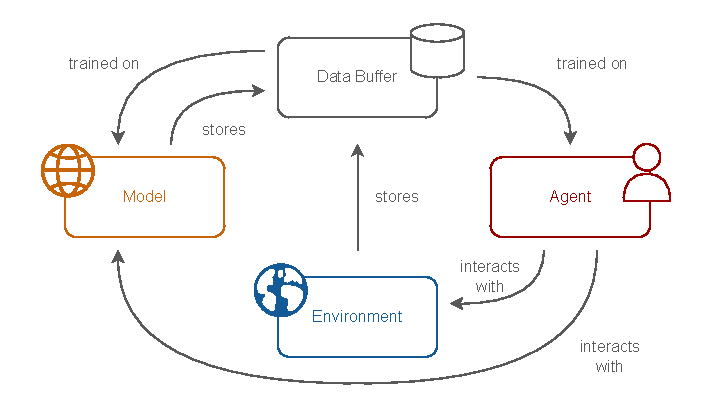
\includegraphics[width=.8\textwidth]{illustrations/thesis_background_dyna.pdf}
    \caption{A sketch of the Dyna framework. The RL agent collects data from the real environment and stores this in a replay buffer. This replay buffer is used to train a model of the environment, which acts as a copy of the environment from the perspective of the agent. Algorithms differ in the question how long model generated data is stored in the replay buffer. While \textcite{janner2019mbpo} for example keeps model generated data for a few thousand update steps, the model-based algorithms presented in \autoref{chap:cvaml} and \autoref{chap:mad} do not store the data for multiple steps at all and generate it anew for each agent update.}
    \label{fig:background:dyna}
\end{figure}


The Dyna framework \parencite{dyna} is one of the most common ways of using an environment model in \ac{rl}.
The main idea is very simple: instead of only using the real environment for generating transition samples $\{x,a,r,x'\}$ we use the model as well.
The concept is sketched out in \autoref{fig:background:dyna}.
In this setup, the use of the model is mostly invisible to the \ac{rl} algorithm which computes the value function and policy.
This makes it very flexible, as we can freely vary the model training and \ac{rl} algorithm without changing the overall framework.

There are several advantages to using the model in addition to the environment.
The simplest is that we are able to generate synthetic data in addition to data from the real environment.
If this data is similar enough to real data, this allows us to increase the sample efficiency of the \ac{rl} training, by simply generating additional data.
Whether this leads to strong performance improvements in applications however depends on how accurate we can make the model with limited data.
If we need as many samples to obtain an accurate model as we need to learn a good value function or policy, the performance gains from Dyna might be limited.

An additional advantage of Dyna is that the model can serve as an oracle simulator.
This means that we can get a next state $\state'$ for any $\state,a$ pair we query the model on.
In the real environment we are instead forced into a sequential interaction where we cannot freely choose the input state $\state$.
\ac{rl} with an oracle generative model can be shown to be optimal in a minimax sense \parencite{agarwal2020model}.
However, the theoretical results rely on obtaining a maximum likelihood model with a well-specified model class.
In practice, we are often not able to learn a sufficiently correct oracle model, and so again, gains in efficiency have to be weighed against model errors influencing the learned value and policy.
We will discuss the impact of model errors on learning extensively in the next section.

As the Dyna framework is relatively flexible, many works in the literature propose algorithms which build on the general idea of learning a model and generating samples from it.
We will review Dyna more closely in \autoref{chap:vagram} and discuss related work.
In \autoref{chap:mad}, we will discuss how using Dyna and specifically the ability to query the model freely with visited states and on-policy actions can greatly stabilize value function learning.

\subsubsection{Online Planning}

While the Dyna framework focuses on improving the value and policies of the agent from stored experiences, a model can also be used to improve the policy as it is being executed.
Depending on the structure of the MDP, proposed methods include random shooting \parencite{pets}, \ac{mcts} \parencite{silver2016mastering,schrittwieser2020mastering}, or \ac{mpc} \parencite{hansen2022temporal,hansen2024tdmpc}.
While the details of the techniques vary, they all follow a similar base formula.

Starting from the current state $\state$ that the agent is in, the agent uses a search policy to query the world model for possible future trajectories.
In the simplest case, random shooting, the agent simply collects $n$ trajectories from the world model by adding random noise to its current policy, or drawing samples from a stochastic policy, and computes the Monte-Carlo estimate of the expected return with regard to the model.
It then executes the most promising action according to these return estimates.
\ac{mcts} and \ac{mpc} can be seen as refinements of this simple techniques where the search procedure is refined by selectively searching over promising future states in the case of \ac{mcts}, or refining the initial action samples iteratively in the case of \ac{mpc}.

In this thesis we will use \ac{mpc}-based methods in \autoref{chap:mad} to improve upon a base policy using a learned model.

\subsubsection{Other ways to use a model}

Beyond learning with Dyna and planning, models can be incorporated into learning in a variety of other ways.
Again, while a thorough survey of model-based reinforcement learning is out of scope for this thesis, we will highlight some additional ideas here as they are relevant for this thesis and related work.

\paragraph{Model-based representation learning:} Instead of using the model directly as an oracle or simulator, a model learning loss can be used to improve the intermediate representations of a neural network-based agent.
This technique is one example of learning with \emph{auxiliary} tasks \parencite{jaderberg2017reinforcement}.
This idea will become an important aspect of this thesis, and will be the focus of \autoref{chap:understanding}.
Therefore we forgo a lengthy introduction here and refer readers to the upcoming chapter.

\paragraph{Differentiating a learned model:} As neural networks have become the de-facto standard way to obtain an environment model in the current machine learning literature, we automatically obtain an additional useful characteristic from this choice: gradients.
As most neural networks are end-to-end differentiable with regard to both their parameters and their inputs, we can use this fact to directly differentiate the model-based return estimate with regard to an action sequence or policy to improve learned policies by differentiating straight through a multi-step bootstrapped rollout.
This technique is succinctly described in \textcite{amos2021model} and used in works such as \textcite{hafner2020dream}.
\textcite{voelcker2022value} discusses differentiable models in the context of decision-aware learning.

\subsection{Abstract latent value models}

\textcite{silver2017predictron} introduced the idea of a purely abstract latent space model in which the transitions is aligned with the reward and value functions of the environment.
Their work considers an uncontrolled setting, in which an action-independent Markov Reward Process (MRP) is modelled.
The goal of their system is to learn the reward function of this process, which can be seen as doing policy evaluation in an \ac{mdp}  with a fixed policy.
The core difference of their approach to other model-based reinforcement learning approaches is that they learn an abstract transition model where the states do not have a one-to-one correspondence to the environment observations.

Extending their work, \textcite{oh2017value} show how to build an abstract model of a fully controllable \ac{mdp}  and highlight how such a model can be used for planning in latent space with a tree search approach such as \ac{mcts} \parencite{schrittwieser2020mastering} or beam search.

\section{Objective mismatch phenomenon}

\label{chap:background:objective}

One of the most important insights that form the basis of this thesis is the fact that model training objectives such as \ac{mle} are not aligned with the objective of \emph{training a good model for \ac{rl}} \parencite{schneider1997exploiting,joseph2013reinforcement,vaml,lambert202objective}.
As a simple example, assume a Dyna setting where a sample is collected from a deterministic model and has an error $\epsilon$.
A value function based method will use the model sample to compute a biased bootstrap target
\begin{align}
    Q_k(\state,a) = r(\state,a) + \gamma Q_{k-1}(f(\state, a) + \epsilon).
\end{align}

The impact of the modelling error on the value function therefore depends both on the size of the error and the local behavior of the value function, and not only on the size of $\epsilon$. 
We could colloquially say that not all errors are created equal.

As another illustrative example, we can imagine a value function that only depends on a subset of all state observation dimensions. 
In this case, a large error in an irrelevant dimension has no consequence on the obtained policy, yet a maximum likelihood loss for the model cannot properly capture this behavior without prior handcrafted features.
Such cases are discussed in more detail in \autoref{chap:understanding} and \autoref{chap:vagram}.

Intuitively, we would like to have an objective that bounds the difference in the value function estimate.
We can motivate the use of an \ac{mle}-based loss function (e.g. the mean squared error for a Gaussian model with fixed variance) {by an upper bound}
$$\sup_{V \in \mathcal{F}}|\langle p - \hat{p}, V\rangle|\leq \|p - \hat{p}\|_1 \sup_{V \in \mathcal{F}}\|V\|_\infty \leq \sqrt{\text{KL}(p|\hat{p})}\sup_{V \in \mathcal{F}}\|V\|_\infty,$$
(taken from
\textcite{vaml}), where the second inequality is Pinsker's inequality.
However, this bound is loose and does not account for the geometry of the problem's value function or any other knowledge that the agent has collected. 
In our example above a mean squared error would penalize deviations equally by their $L_2$ norm without accounting for the relevance of the dimensions.
This problem was termed the \emph{objective mismatch} by \textcite{lambert202objective}.

To refer to our goal of learning models which mitigate the mismatch, we will use the terms ``decision-aware'' and ``value-aware'' mostly interchangeably.
Both terms were introduced by \textcite{vaml}.
The former refers more generally to algorithms and models which account for the downstream decision task, while the latter refers more concretely to algorithms and models which account for errors in the value function target estimate.
However, in this thesis our main focus is on value function learning, which means we mostly use decision-awareness in the more narrow sense of value-aware learning.

\subsection{Value-aware model learning}

To address the model mismatch, \textcite{vaml} proposed \emph{Value-aware Model Learning} (VAML), a loss function that captures the impact the model errors have on the one-step value estimation accuracy.
The core idea behind VAML is to penalize a model prediction by the resulting difference in a value function. Given a distribution over the state-actions space $\mu$ and a value function $V$, it is possible to define a value-aware loss function $\mathcal{L}_V(\hat{p}, p, \mu)$
\begin{align}
    &\mathcal{L}_V(\hat{p}, p, \mu) = \int \mu(\state,a) \bigg|\underbrace{\int p(\state'|\state,a)V(\state')\mathrm{d}\state'}_{\text{environment value estimate}}  - \underbrace{\int \hat{p}(\state'|\state,a) V(\state') \mathrm{d}\state'}_{\text{model value estimate}}\bigg|^2 \mathrm{d} (\state,a).
\end{align}
and its empirical approximation $\hat{\mathcal{L}}_V$ based on a dataset $D = (\state_i,a_i,\state'_i)_{i=1}^N$ of samples from $\mu$ and $p$
\begin{align}
    &\hat{\mathcal{L}}_V(\hat{p}, \mathcal{D}) = \frac{1}{|D|}\sum_{(\state_i,a_i,\state'_i)\in\mathcal{D}} \left|V(\state'_i) - \int \hat{p}(\state'|\state_i,a_i) V(\state') \mathrm{d} \state'\right|^2\label{eq:background:IterVAMLloss}.
\end{align}

The main problem of this approach is that it relies on the value function, which is not known a priori while learning the model. 
This leads to the "chicken-egg" problem of decision aware learning which will be the focus of \autoref{chap:vagram}:

\begin{quote}
    {If a good model depends on knowing the correct decisions and good decisions need to be learned using the model, how can we learn a good model before knowing what the correct decision is?}
\end{quote}

In the original formulation by \textcite{vaml}, the value function is the supremum over a function space $\mathcal{V}$ to enable analysis
\begin{align}
    &\mathcal{L}_\text{VAML}(\hat{p}, p, \mu) = \int \mu(\state,a) \sup_{V\in \mathcal{V}}\bigg|\int p(\state'|\state,a)V(\state')\mathrm{d}\state'  - \int \hat{p}(\state'|\state,a) V(\state') \mathrm{d}\state'\bigg|^2 \mathrm{d} (\state,a).
\end{align}

While this evades the chicken-egg problem of decision-aware model learning and leads to tractable analysis in the case of linear value function spaces, finding a supremum for a function space parameterized by complex function approximators like neural networks is difficult.
Furthermore, the supremum formulation is conservative and does not account for the fact that knowledge about the value function is gained over the course of exploration and optimization in an \ac{mbrl} approach.

Instead of the supremum over a value function class, \textcite{itervaml} introduced \emph{Iterative Value-Aware Model Learning} (IterVAML) where the supremum is replaced with the current estimate of the value function.
In each iteration, the value function is updated based on the model, and the model is trained using the loss function based on the last iteration's value function.
The author presents error bounds for both steps of the iteration, but did not test the algorithm to ascertain whether the presented error bounds are sufficient to guarantee a strong algorithm in practice. 
Furthermore, these work assume that both the Approximate Value Iteration and model learning procedure are conducted until they reach a small error at every step, which is often prohibitively expensive, or even impossible in case of neural network value function approximations.
We will look at IterVAML more extensively in \autoref{chap:vagram} and \autoref{chap:cvaml}.



\section{Representation learning in RL}

The main goal of learning useful representations is to capture some desirable characteristic with regards to a prediction task in the latent space.
This is often some form of smoothness or (Lipschitz)-continuity, or come optimal compression compression.
\textcite{abel2020thesis} and \textcite{le2021metrics} provide excellent overviews of the general goals of representations in the context of \ac{rl}.

One of the major components of the success of Deep Learning has been the surprising capability of neural networks to \emph{learn} good representations for tasks such as classification \parencite{bengio2012representation}.
One of the most prominent examples are the structured latent spaces obtained by the word2vec algorithm, where training to predict (embeddings of) words leads to structured spaces that allow for meaningful vector arithmetic \parencite{mikolov2013distributed,goldberg2014word2vec}.

The core challenges for representation learning in \ac{rl} is that the tasks are fundamentally non-stationary in nature \parencite{kumar2021implicit,nikishin2022primacy}.
As the agent explores the environment, value function and policy continually change, meaning that both the input distribution and the prediction targets change over time.
This has led to the establishment of research into \emph{learning dynamics} \parencite{lyle2022learning,lyle2022understanding}, \emph{metric learning} \parencite{ferns2011bisimulation,zhang2021learning,le2021metrics,kemertas2022approximate}, \emph{successor features} \parencite{barreto2017successor,borsa2018universal}, and \emph{auxiliary tasks} \parencite{jaderberg2017reinforcement,bellemare2019geometric,lyle2021effect,farebrother2023protovalue} to address these challenges.

\subsubsection{Desirable properties of representations}

Before discussing how representation learning in RL can be improved, it is necessary to characterize representations that lead to good performance in \ac{rl}.
As discussed above, in many classic \ac{rl} approaches, the state space is taken to be a finite set of unordered states without any metric or distance between these except for the one induced by the transition function.
Over such abstract states, one of the most commonly considered representations is a state aggregation.
State aggregations are thoroughly discussed by \textcite{abel2020thesis}, where three core desiderata are established: good state aggregations should be easy to compute, enable efficient learning, and allow the selection of high-value policies.

Beyond state abstraction, the topology and metric of the representation space can also be considered. 
\textcite{le2021metrics} and \textcite{lelan2022generalization} discuss the capabilities of representations to enable generalization of learned value functions over the state space by analyzing the induced topology and metric space induced by different representation learning approaches.
Their work allows us to consider the impact of the representation on the learning dynamics and generalization capabilities of different algorithms.

\textcite{ghosh2020representations} extends the analysis of representation beyond fixed properties such as metric spaces to consider the impact of the given representation on the stability of the learning task.
Using tools from linear dynamical system, they show that some proposed representations provide more stable learning dynamics for TD-learning as others.

\subsubsection{General-purpose representation learning}

To obtain optimal representations for reinforcement learning tasks in a given environment without a specific reward function, several different approaches have been proposed.
In the nomenclature of this thesis, these are \emph{general-purpose} representation learning methods.
Several of the leading approaches are inspired from linear algebra and graph theory and seek to model fundamental aspects of the transition matrix.

Broadly speaking, the transition matrix $\mathcal{P}$ and the resolvent matrix $(I - \gamma \mathcal{P})^{-1}$ can be approximated by different decompositions such as eigenvalue decompositions, singular value decomposition, or Schur decomposition \parencite{mahadevan2005proto,mahadevan2007proto,ghosh2020representations}.
These matrix approximations can then be used to obtain e.g. the largest eigenvectors which capture the long-term transition behavior of the underlying Markov chains.
For example, the equality $V = (I - \gamma \mathcal{P})^{-1} r$ shows that if the resolvent matrix is well approximated, a representation can be obtained that can be used to approximate the value function of any reward.
These decompositions and how they emerge from tractable prediction objectives will be discussed in detail in \autoref{chap:understanding}.

The goal of obtaining well-performing representations has also been addressed with empirically motivated approaches.
Many of these seek to construct so called \emph{auxiliary tasks} \parencite{jaderberg2017reinforcement}, which are additional prediction objectives or loss functions which are added to the learning objectives of the RL agent.
These generally do not take the reward or value prediction objectives into account.
Such auxiliary tasks can be constructed using auto-encoder architectures \parencite{jaderberg2017reinforcement}, contrastive learning \parencite{laskin2020contrastive}, or self-supervised objectives \parencite{gelada2019deepmdp,schwarzer2021dataefficient,schwarzer2021pretraining,tang2022understanding}.
These methods tend to be especially important in cases with high-dimensional observations, i.e. as pixel based environments such as Atari games, or sparse rewards.
The main distinction between these methods and \ac{mbrl} is that the next state prediction is only used to improve the performance of an encoder function.
Next state predictions are not directly used to improve the RL agents policy or value function estimation.
We will analyze several types of auxiliary tasks in detail in \autoref{chap:understanding}.

Beyond state prediction tasks, several works have also shown the advantage of using value function prediction of auxiliary or randomly generated rewards as representation learning targets \parencite{lyle2021effect,farebrother2023protovalue}.
These commonly use the same approaches as off-policy value function learning, but instead of using the estimated value functions to derive a policy, the results are again discarded and only used for stabilization.
As we will discuss in \autoref{chap:understanding}, many of these approaches lead to features which are closely related to features obtained from self-supervised predictions.

\section{Decision-aware vs general-purpose learning}
\begin{figure}[t]
    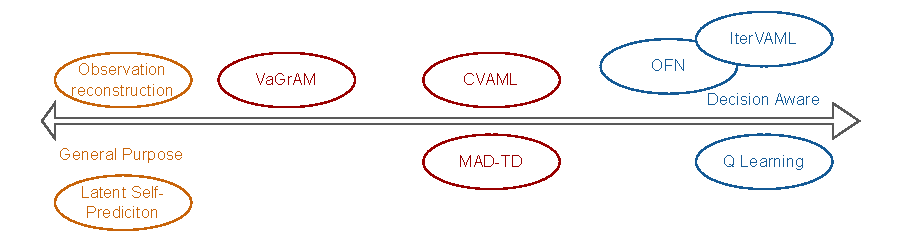
\includegraphics{illustrations/thesis_daml_spectrum.pdf}    
    \caption{A visual representation of the spectrum between decision-aware and general purpose learning.
    Several approaches presented in this thesis, such as VaGraM (\autoref{chap:vagram}), CVAML (\autoref{chap:cvaml}), and MAD-TD (\autoref{chap:mad}) combine methods from both general purpose and decision-aware learning to achieve stable and efficient \ac{rl}.
    OFN (\autoref{chap:overestimation}) only consider model-free RL and can therefore be seen as a purely decision-aware method.
    Finally, while latent self-prediction and observation reconstruction are general purpose methods, \autoref{chap:understanding} investigates how they can be used in synergy with TD learning.
    Based on this investigation, latent self-prediction is used to obtain a strong hybrid methods such as MAD-TD.}
    \label{fig:background:spectrum}
\end{figure}

The major problem that motivates the work conducted in this thesis is that the current value function alone does not necessarily provide sufficient information to learn good representations or world models.
As discussed in the introduction, reinforcement learning is fundamentally non-stationary in nature, which means that the current prediction task is not necessarily indicative of future prediction tasks.

To understand the problem intuitively, a sparse reward setting is instructive: when the task requires exploration, the value function is driven to predict $0$ for all visited states until the agent has actually reached the goal and observed positive reward.
A model or representation can then collapse the whole state space into a single feature, as no value other than 0 needs to be predicted, and potentially completely prevent further exploration.

This phenomenon is for example partially discussed by \textcite{tomar2023learning}, who show that many techniques for value-based abstractions fail in hard-exploration scenarios.
Similarly, \textcite{kemertas2021towards} show that auxiliary training objectives strongly improve the performance of bisimulation-based representation learning, especially with sparse rewards.
A related discussion in the the context of IterVAML will be presented in \autoref{chap:vagram}.
Finally, \textcite{nikishin2022primacy} conjecture the existence of a \emph{primacy bias}, the tendency of neural network-based value functions to overfit initial experience and to lose capacity to represent information obtained later in training.
This notion of the primacy bias will be addressed in detail in \autoref{chap:overestimation} and \autoref{chap:mad}, and we will see that the primacy bias can be related to the problems of learning representations and models from purely decision-aware objectives.

However, while decision-aware methods face challenges with stability, their great advantage lies in the fact that they can adapt to the task.
While general-purpose methods are often more robust to shifts in the task and missing value information, they fail to be as efficient as the latter especially under resource constraints such as network size.
Examples of this are presented in \autoref{chap:understanding} and \autoref{chap:vagram} where we see the benefits of using decision-aware algorithms when the observation space contains irrelevant distracting dimensions.
Therefore, instead of exploring decision-awareness and general-purpose learning as opposing ideas, this thesis is instead looking to find synergy which allows us to take advantage of both paradigms.
This idea is visualized in \autoref{fig:background:spectrum}, where the approaches presented in this thesis are roughly visualized along a spectrum between general-purpose and decision-aware learning.


    \chapter{Instability of value function learning}

\section{Introduction} \label{sec:intro}

To improve sample efficiency, contemporary work in off-policy deep reinforcement learning (RL) has begun increasing the number of gradient updates per collected environment step~\parencite{janner2019mbpo,fedus2020revisiting,chen2021randomized, hiraoka2022dropout, nikishin2022primacy, doro2023barrier, schwarzer2023bigger, kim2023resetensemble}.  
As this update-to-data (UTD) ratio increases, various novel challenges arise.
Notably, a recent study proposed the emergence of a \emph{primacy bias} in deep actor critic algorithms, defined as ``a tendency to overfit initial experiences that damages the rest of the learning process''~\parencite{nikishin2022primacy}. 
This is a fairly broad explanation of the phenomenon, leaving room for investigation into how fitting early experiences causes suboptimal learning behavior.

First approaches to tackle the learning failure challenges have been suggested, such as completely resetting networks periodically during the training process and then retraining them using the contents of the replay buffer~\parencite{nikishin2022primacy, doro2023barrier}. 
Resetting network parameters is a useful technique in that, in some sense, it can circumvent any previous optimization failures without prior specification. 
Yet it seems likely that a more nuanced treatment of the various optimization challenges in deep RL might lead to more efficient training down the line. 
Especially if the objective is efficiency, throwing away all learned parameters and starting from scratch periodically is counter-productive, for instance in scenarios where, keeping all previous experience is infeasible. %for instance when data buffer sizes become limited. 
As such, we set out to study the components of early training that impair learning more closely and examine whether high-UTD learning without resetting is possible. 


To motivate our study, we repeat the priming experiment of \textcite{nikishin2022primacy}, in which a network is updated for a large number of gradient steps on limited data. We show that during priming stages of training, value estimates diverge so far---and become so extreme---that it takes very long to unlearn them using new, counter-factual 
data. However, contrary to prior work, we find that it is not \emph{impossible} to learn even after priming, it merely takes a long time and many samples. 
This sparks hope for our endeavor of smooth learning in high-UTD regimes.
We show that compensating for the value function divergence allows learning to proceed. This suggests that the failure to learn does not stem from overfitting early data, which would result in correct value function on seen data, but rather from improperly fitting Q-values. 
% This can be traced to bootstrapping of poorly specified Q-function networks on unseen data. 
We demonstrate that this divergence is most likely caused by prediction of out-of-distribution (OOD) actions that trigger large gradient updates, compounded by the momentum terms in the Adam optimizer~\parencite{kingma2015adam}.
% While there are standard approaches that have been proposed to solve the issue of overestimation, our experiments highlight that these come with unwanted side effects in the high update-to-data ratio setting with limited data. 

The identified behavior, although triggered by OOD action prediction, seems to be more than the well-known overestimation due to statistical bias \parencite{thrun1993issues}. 
Instead, we hypothesize that the problem is an optimization failure and focus on limiting the exploding gradients from the optimizer via architectural changes.
The main evidence for this hypothesis is that standard RL approaches to mitigating bias, such as minimization over two independent critic estimates~\parencite{fujimoto2018addressing}, are insufficient. In addition, using pessimistic updates~\parencite{fujimoto2019bcq, fujimoto2021td3bc} or regularization~\parencite{krogh1991simple, srivastava14dropout} to treat the value divergence can potentially lead to suboptimal learning behavior, which is why architectural improvements are preferable in many cases.

% Combating overestimation is a problem with a long history in both value-based and actor-critic approaches, but our findings suggest that the most common approach (minimization over two independent critic estimates)  is insufficient, especially in the high UTD regime.

We use a simple feature normalization method \parencite{zhang2019root, wang2020striving, bjorck2022is} that projects features onto the unit sphere.
This decouples learning the scale of the values from the first layers of the network and moves it to the last linear layer.
Empirically, this approach fully mitigates diverging Q-values in the priming experiment. Even after a large amount of priming steps, the agent immediately starts to learn. %, rendering resetting unnecessary. 
In a set of experiments on the \textsf{dm\_control} MuJoCo benchmarks~\parencite{tunyasuvunakool2020dmcontrol}, we show that accounting for value divergence can achieve significant across-task performance improvements when using high update ratios. 
Moreover, we achieve non-trivial performance on the challenging dog tasks that are often only tackled using model-based approaches. We demonstrate comparable performance with the recently developed TD-MPC2~\parencite{hansen2024tdmpc}, without using models or advanced policy search methods.
Lastly, we isolate more independent failure modes, giving pointers towards their origins. In Appendix~\ref{app:open} we list open problems whose solutions might illuminate other RL optimization issues.


\section{Preliminaries} \label{sec:preliminaries}

\section{Investigating the effects of large update-to-data ratios during priming} \label{sec:investigating}

\begin{figure}[t!]
% \captionsetup[subfigure]{font=footnotesize, aboveskip=2pt}
\centering
    \begin{subfigure}[b]{0.8\textwidth}
        \centering
        
\includegraphics[height=0.4cm]{figures/dissecting/priming/priming_base_return_legend.pdf}
    \end{subfigure}\\%
    \begin{subfigure}[b]{0.25\textwidth}
        \centering
        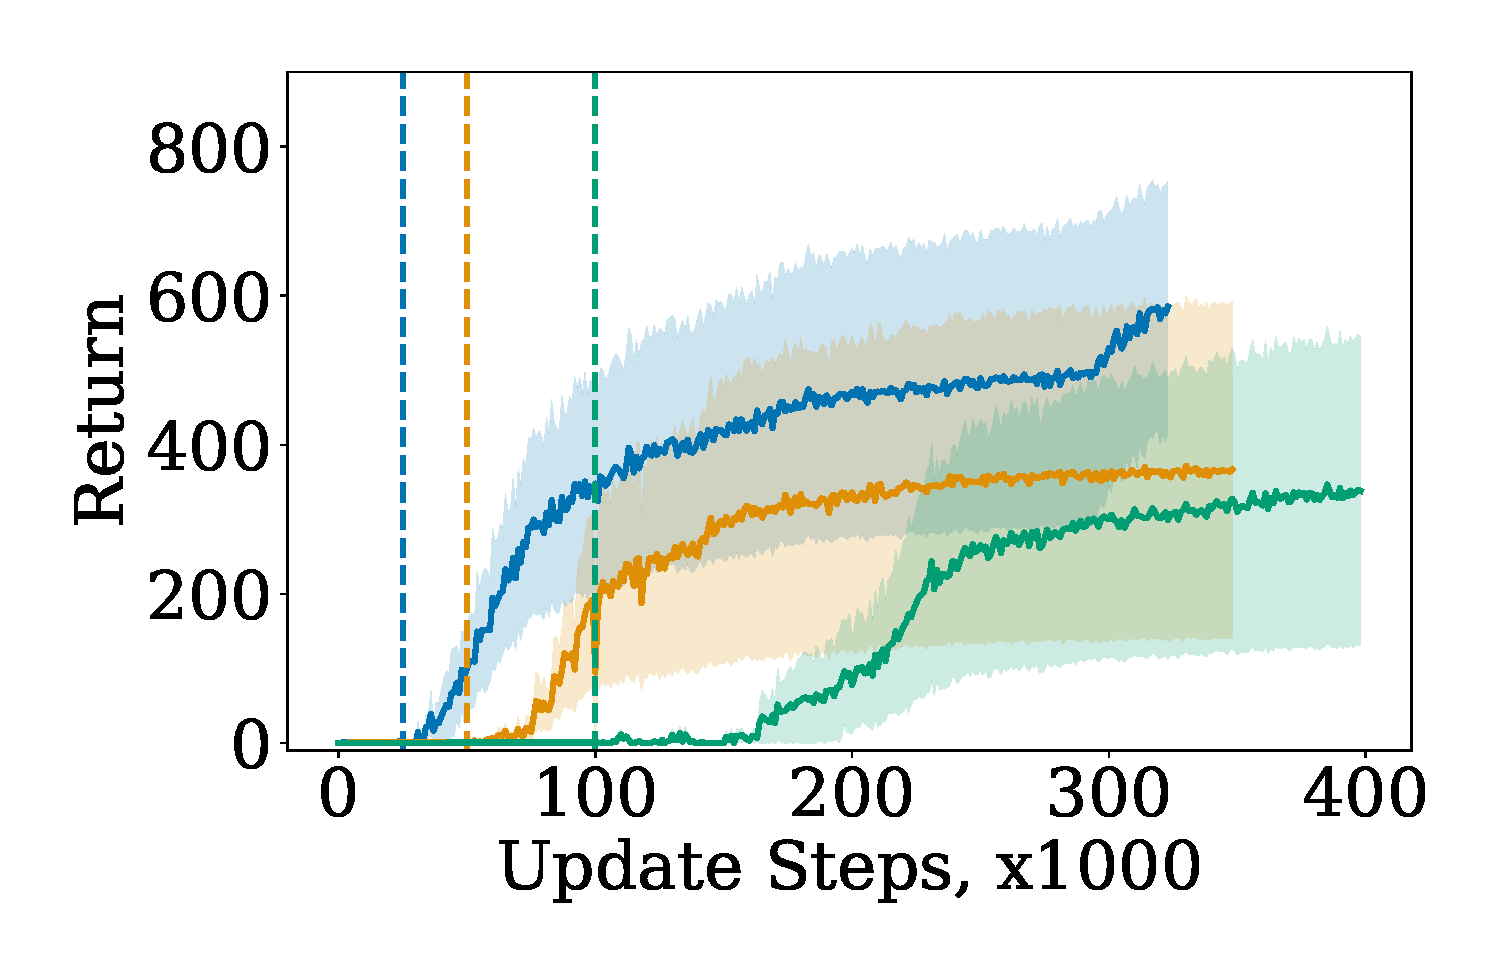
\includegraphics[width=3.7cm, trim=1cm 1cm 1cm 1cm ,clip]{figures/dissecting/priming/priming_base_return.pdf}
        \label{subfig:priming_base_ret}
    \end{subfigure}%
    \begin{subfigure}[b]{0.25\textwidth}
    \centering
        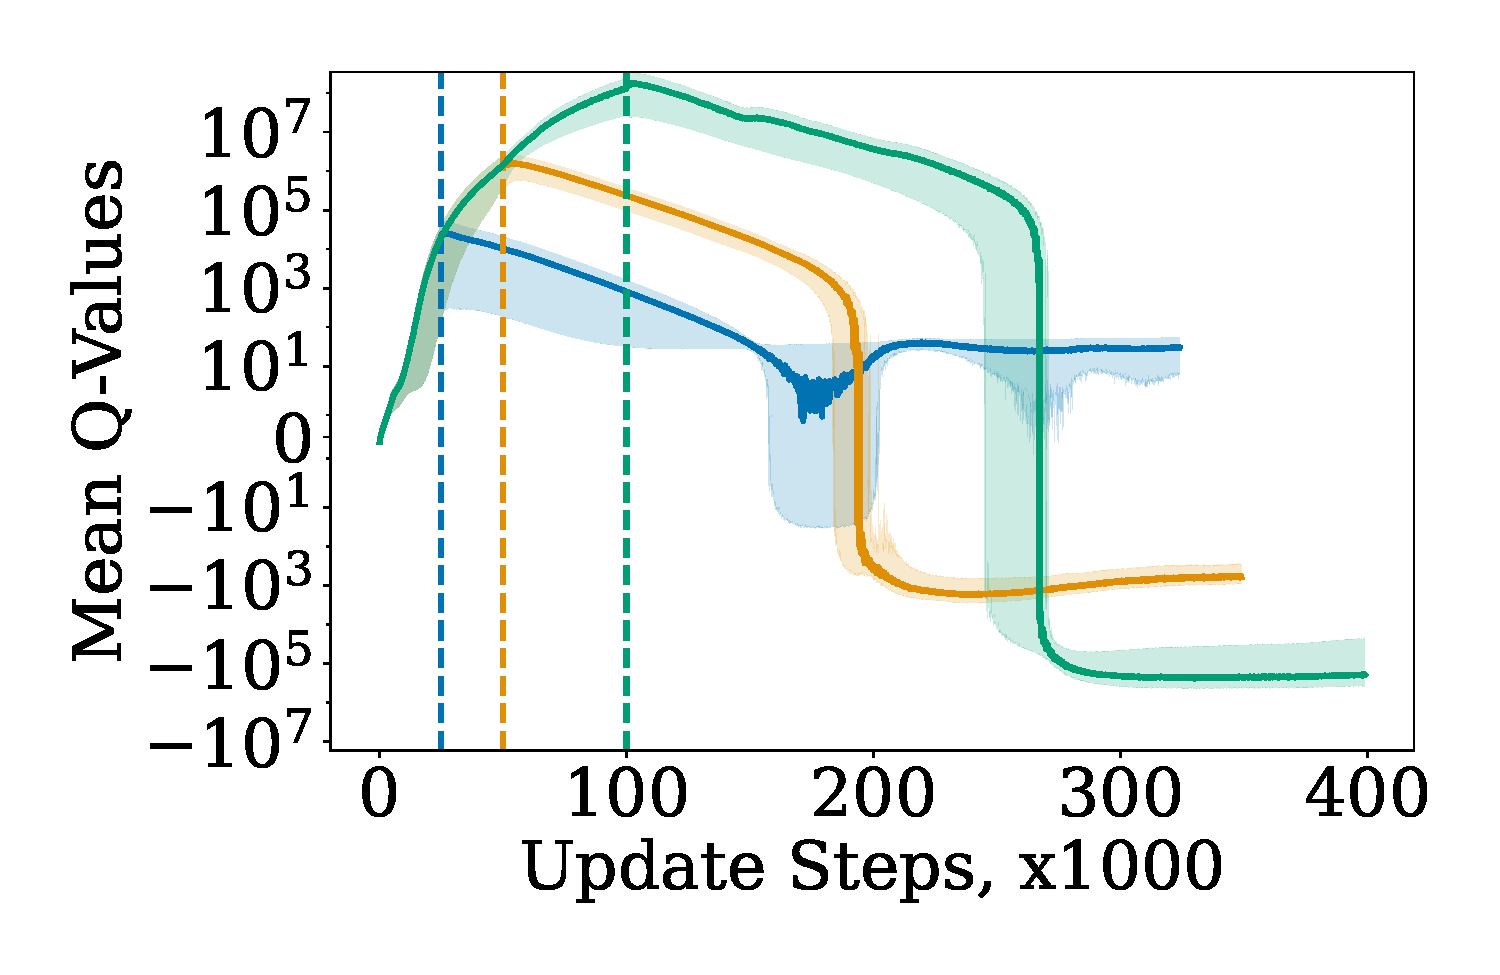
\includegraphics[width=3.7cm, trim=1cm 1cm 1cm 1cm ,clip]{figures/dissecting/priming/priming_base_Q.pdf}
        \label{subfig:priming_base_Q}
    \end{subfigure}%
    \begin{subfigure}[b]{0.25\textwidth}
        \centering
        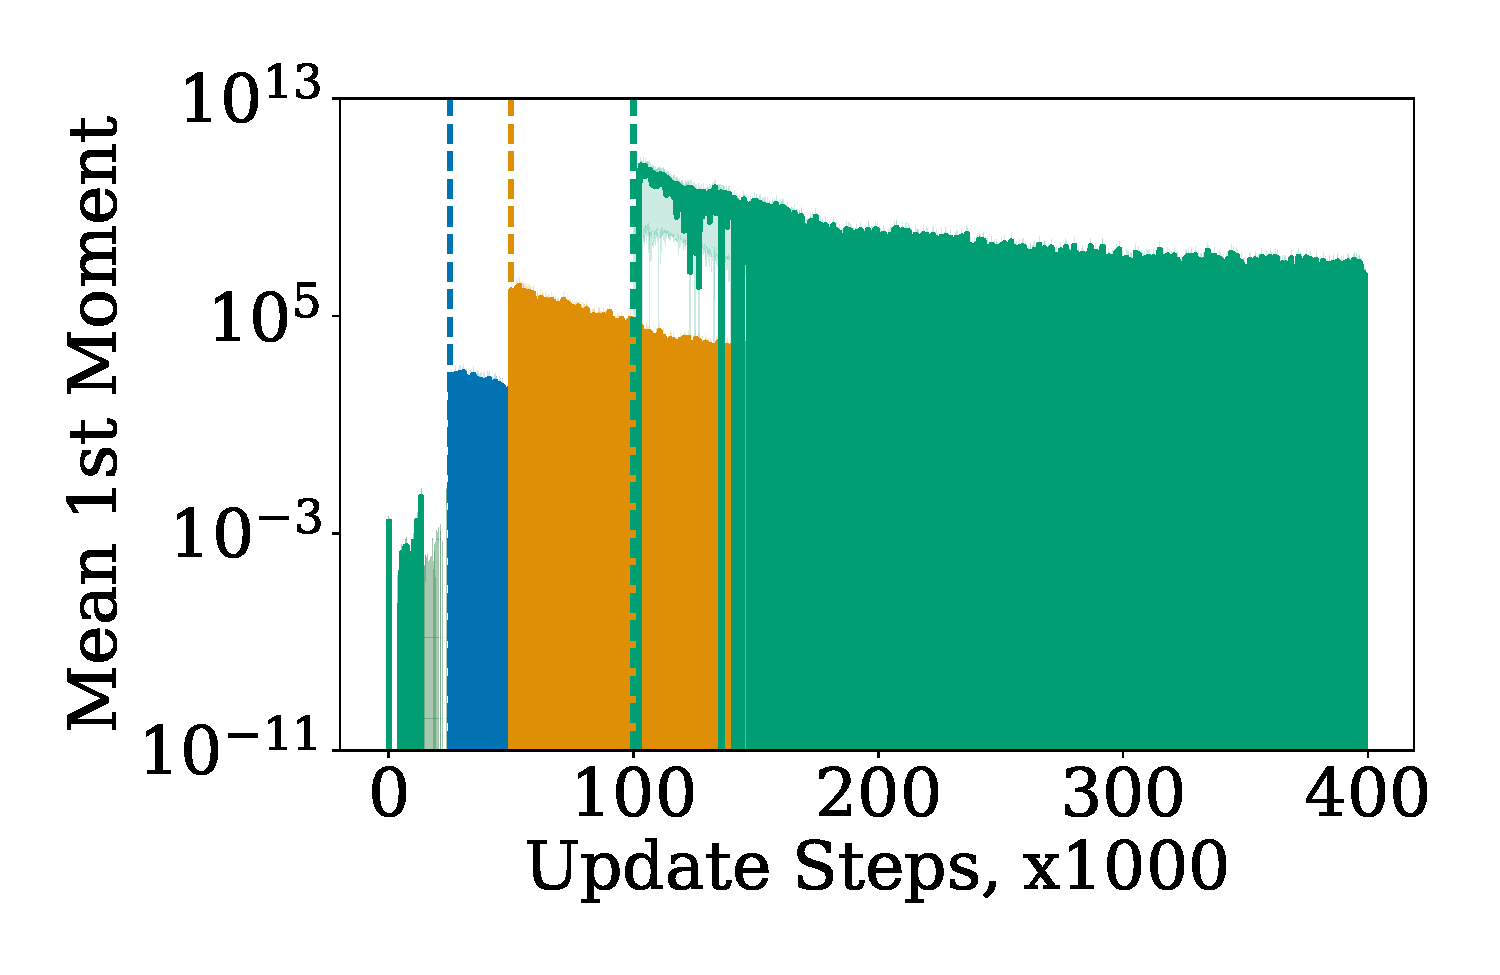
\includegraphics[width=3.7cm, trim=1cm 1cm 1cm 1cm ,clip]{figures/dissecting/priming/priming_base_exp_avg.pdf}
        \label{subfig:priming_base_mom}
    \end{subfigure}%
    \begin{subfigure}[b]{0.25\textwidth}
        \centering
        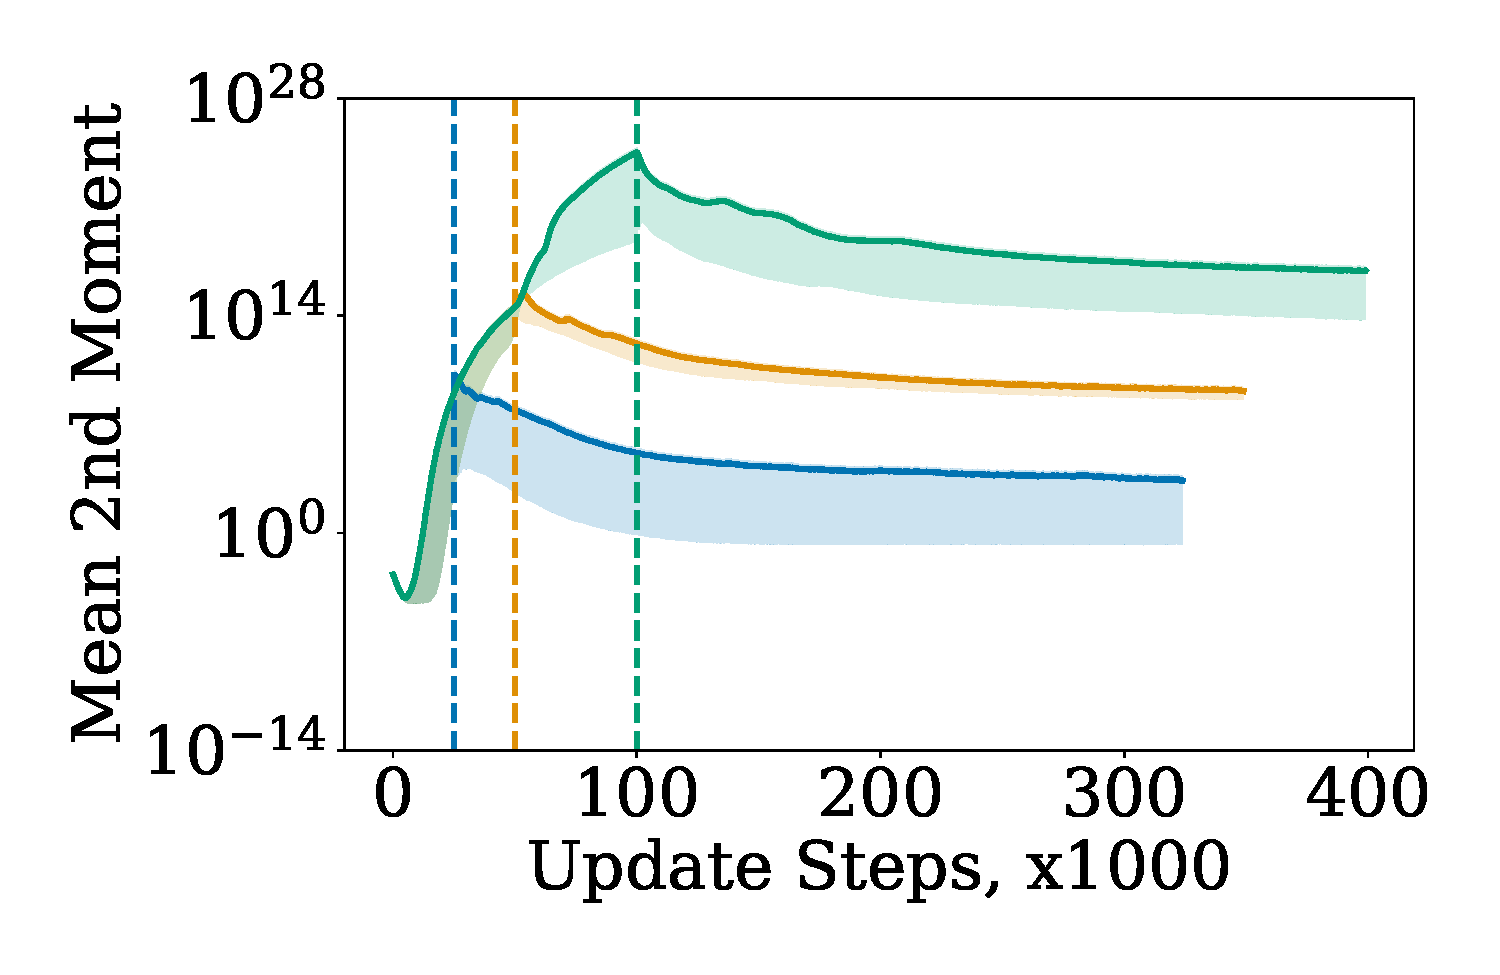
\includegraphics[width=3.7cm, trim=1cm 1cm 1cm 1cm ,clip]{figures/dissecting/priming/priming_base_exp_avg_sq.pdf}
        \label{subfig:priming_base_mom}
    \end{subfigure}%
    \vspace{-5pt}
    \caption{Return, in-distribution Q-values and Adam optimizer moments during priming for different lengths. Dotted lines correspond to end of priming. More priming leads to lower return and larger Q-value and optimizer divergence.}
    % \caption{Mean return, Q-values and Adam moments for priming of different lengths. Dotted lines indicate end of priming. More priming leads to lower return and Q-value and optimizer divergence.}
    \label{fig:priming_base}
\end{figure}

As mentioned, the definition of the primacy bias is broad.
To obtain a more nuanced understanding, we set out to re-investigate the early stages of high-UTD training. To do so, we repeat the priming experiment conducted by~\textcite{nikishin2022primacy}.\footnote{For consistency with later sections, we use the ReLU activation here which can lead to unstable learning of other components. We repeat all the experiments with ELUs in Appendix~\ref{app:priming} to provide even stronger support of our findings.}
We first collect a small amount of random samples. Then, using the SAC algorithm, we perform a priming step, training the agent for a large number of updates without additional data. After priming, training continues as usual. Prior results reported by~\textcite{nikishin2022primacy} suggest that once the priming step has happened, agents lose their ability to learn completely. We use the simple Finger-spin task \parencite{tunyasuvunakool2020dmcontrol} to study the root causes for this systematic failure and to examine if there are ways to recover without resets. In this section, we report means over five random seeds with standard error in shaded regions. Hyperparameters are kept consistent with previous work for ease of comparison.
% \mh{we should maybe add something about more stable results from elu in appendix}

\subsection{An old acquaintance: Q-value overestimation} \label{sec:overestimation}
We first ask whether there is a barrier as to how many steps an agent can be primed for before it becomes unable to learn. We test this by collecting 1,000 samples and varying the number of updates during priming from 25,000 to 50,000 and 100,000. The results are presented in Figure~\ref{fig:priming_base}. 

We make two key observations. First, lower amounts of priming are correlated with higher early performance. More precisely, it seems that many runs simply take longer before they start learning as the number of priming steps increases. Second, during priming the scale of the average Q-value estimates on observed state-action pairs increases drastically. We find that the Q-values start out at a reasonable level, but as priming goes on they eventually start to diverge drastically. Once the agent estimates very large Q-values, the final performance in terms of average returns deteriorates. We also observe that the second moment of the Adam optimizer~\parencite{kingma2015adam} is correlated with the divergence effect. Optimizer divergence has been observed before as a cause of plasticity loss under non-stationarity~\parencite{lyle2023understanding}, but in our experiments the data is stationary during priming. We conjecture that the momentum terms lead to much quicker propagation of poor Q-values and ultimately to prediction of incorrect Q-values, even on in-distribution data.

% However, without regularization it seems that once the effective dimension falls below a certain threshold, agents take substantially longer to recover and learning becomes essentially impossible (see Appendix~\ref{todo}). 

After priming, there exist two cases: 1) either the Q-values need to be unlearned before the agent can make progress or 2) there is a large drop from very high to very low Q-values that is strongly correlated with loss in effective dimension of the embedding, as defined by~\cite{yang2020harnessing} (see Appendix~\ref{app:priming_dim}). In the second case, rank can sometimes be recovered upon seeing new, counter-factual data and the network continues to learn. Yet, sometimes the agent gets stuck at low effective dimension; a possible explanation for the failure to learn observed in the priming experiments of~\textcite{nikishin2022primacy}. This is orthogonal to a previously studied phenomenon where target network-based updates lead to perpetually reduced effective rank~\parencite{kumar2021implicit}.

%However, the priming experiment alone does not allow us to conclude whether overestimation is a symptom or a cause of the primacy effect.
% To differentiate, we need a way to either prevent capacity loss in the network, or to regularize the Q values as to control for the impact of one or the other. 

% When looking at the resetting results in~\textcite{nikishin2022primacy, doro2023barrier}, several interesting observations can be made. First, it seems that in many cases a large part of the performance gains that are obtained from resetting seem to happen after the first reset. Additionally, after resetting for the first time, the variance across random seeds ostensibly reduces significantly in many of the experiments. \mh{Lastly, it seems unclear when exactly resetting which network should happen.} We set out to explore the cause for these events by considering a similar priming experiment as suggested in~\textcite{nikishin2022primacy}. We collect an initial sample of $2560$ observations from the environment, train for a large number of updates $U$ and this initial set and then return to standard SAC training. In doing so, we vary the number $U$ to artificially create the effects of increased UTD-ratios. 

% \subsection{Q-value divergence as a root cause}

% The results in~\ref{fig:priming} indicate that a key property of the training runs is that with increased $U$, 

% So as long as priming is not too strong, we can live with it. However, we must "unlearn" bad Q-values before we can start learning to solve the task. We hypothesize that resetting helps both to speed-up unlearning as well as getting back from the point of no return. We hypothesize that, if divergence never happens, we never have to do either of these and should simply be able to learn removing the need for expensive retraining after resets.
% Our core observation is that the priming procedure produces strong Q value - not only overestimation but - divergence which up to a certain extent can be combated with more training. 


\subsection{On the potential causes of divergence} \label{sec:causes}

\begin{figure}[t]
\begin{minipage}[b]{.35\textwidth}
% \captionsetup[subfigure]{font=footnotesize, aboveskip=2pt}
\centering
    \begin{subfigure}[b]{\textwidth}
        \centering
        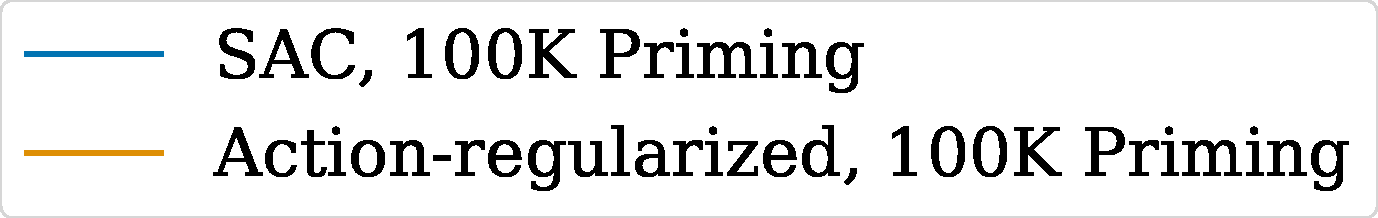
\includegraphics[height=0.8cm]{figures/dissecting/priming/priming_causes_return_legend.pdf}
    \end{subfigure}\\%
    \begin{subfigure}[b]{\textwidth}
        \centering
        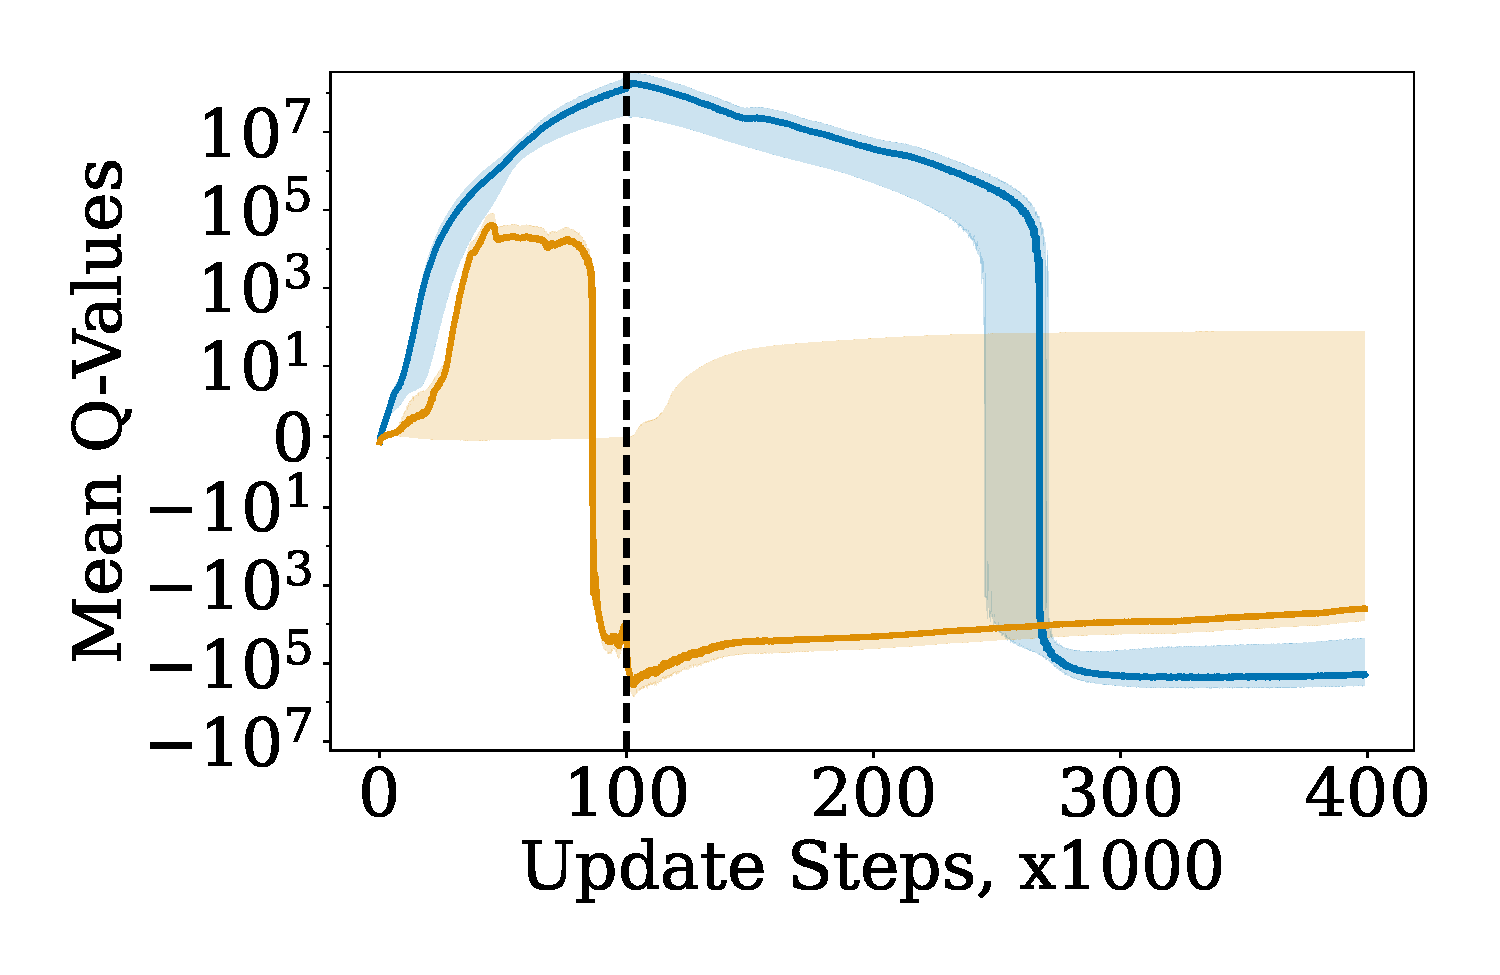
\includegraphics[width=4.8cm, trim=1cm 1cm 1cm 1cm ,clip]{figures/dissecting/priming/priming_causes_Q.pdf}
        \label{subfig:priming_causes_Q}
    \end{subfigure}%
    \vspace{-5pt}
    \caption{Priming with SAC and action regularization during priming. The latter lowers divergence. }
    \label{fig:priming_causes}
\end{minipage}
\hfill
\begin{minipage}[b]{.62\textwidth}
% \captionsetup[subfigure]{font=footnotesize, aboveskip=2pt}
    \centering
    \begin{subfigure}[b]{0.8\textwidth}
        \centering
        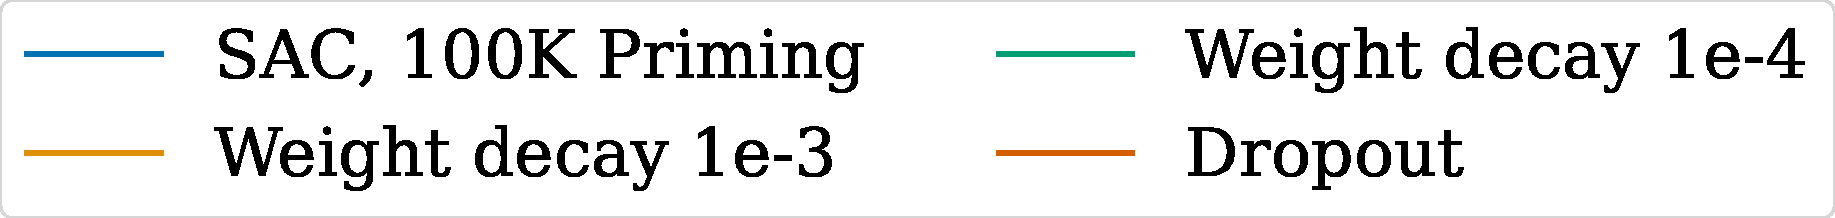
\includegraphics[height=0.8cm]{figures/dissecting/priming/priming_ablations_return_legend.pdf}
    \end{subfigure}\\%
    \begin{subfigure}[b]{0.5\textwidth}
        \centering
        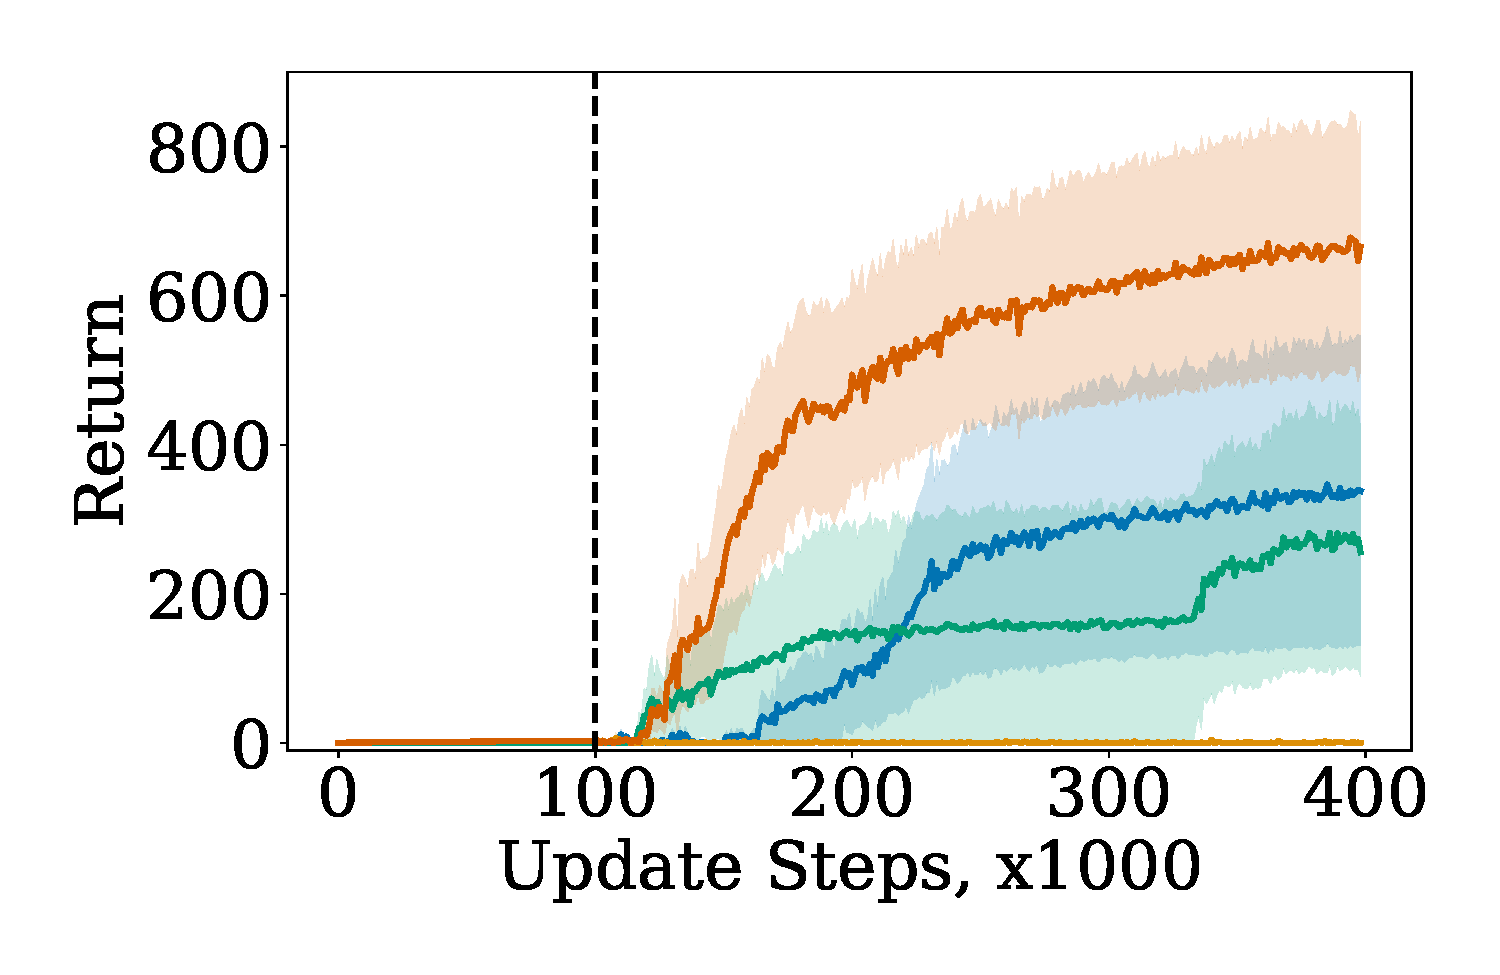
\includegraphics[width=4.8cm, trim=1cm 1cm 1cm 1cm ,clip]{figures/dissecting/priming/priming_ablations_return.pdf}
        \label{subfig:priming_abl_ret}
    \end{subfigure}%
    \begin{subfigure}[b]{0.5\textwidth}
    \centering
        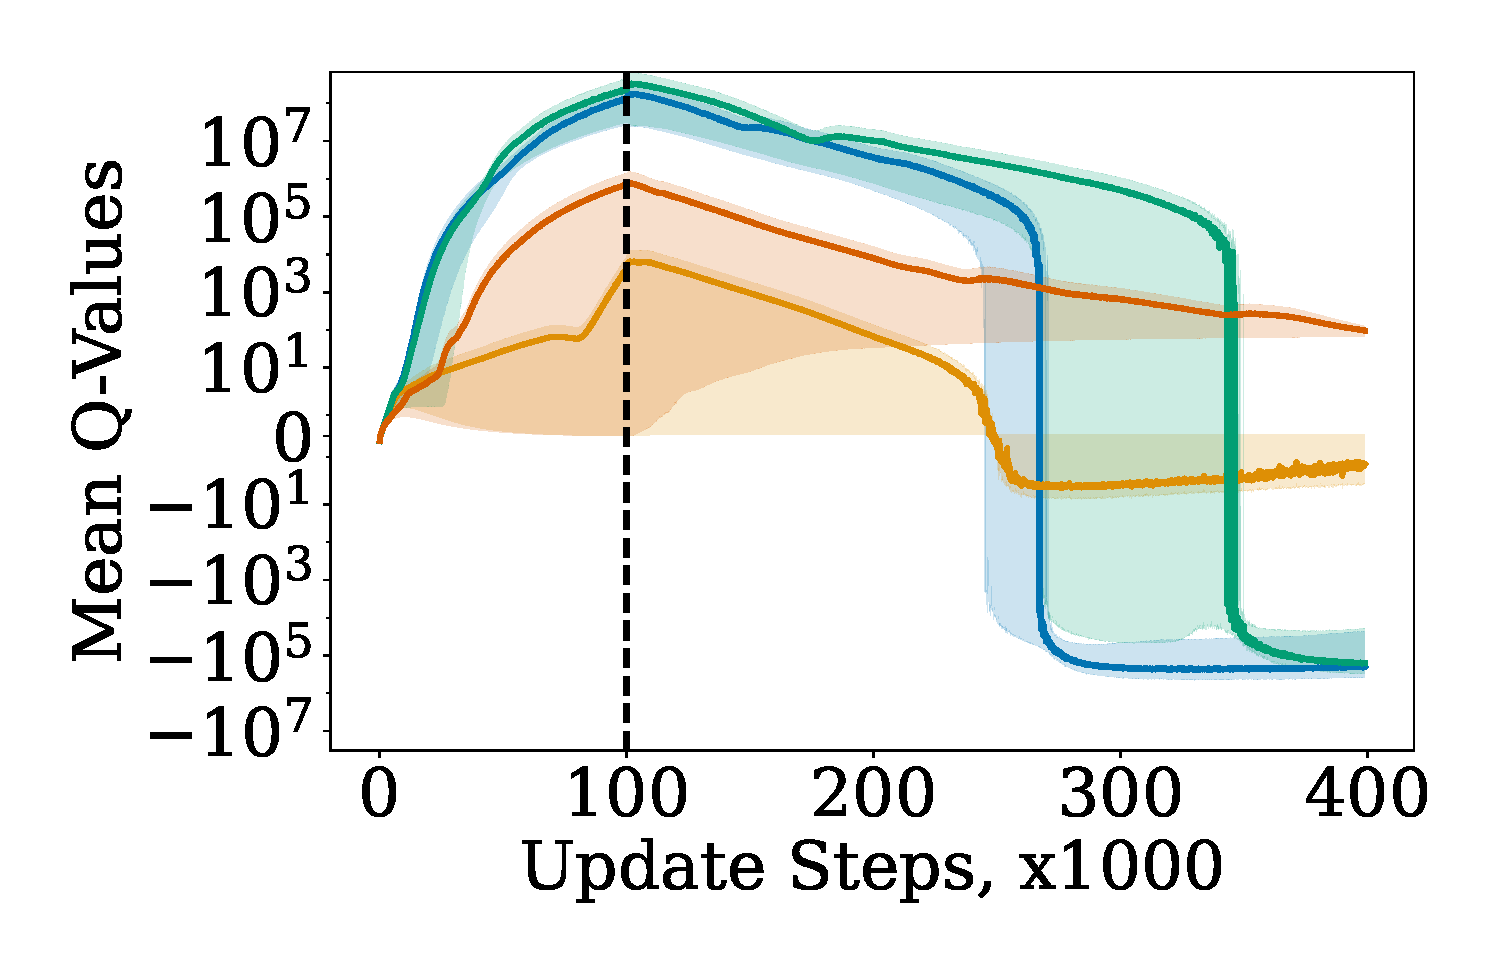
\includegraphics[width=4.8cm, trim=1cm 1cm 1cm 1cm ,clip]{figures/dissecting/priming/priming_ablations_Q.pdf}
        \label{subfig:priming_abl_Q}
    \end{subfigure}%
    \vspace{-18pt}
    \caption{Return and
    Q-values of priming runs with weight decay and dropout. Results indicate that both regularizations mitigate priming to some extent but not sufficiently. }
    \label{fig:priming_abl}
\end{minipage}
    \vspace{-5pt}
\end{figure}

% A well-known phenomenon that was already identified in the early stages of reinforcement learning research is that trying to find a value function via function approximation can quickly lead to overestimates of said values~\textcite{thrun1993issues}. This overestimation of the value function remains a challenge even for modern algorithms like SAC, due to the hurdles that emerge with what is often referred to as the \emph{deadly triad}: function approximation, reliance on bootstrap updates and off-policy data in the form of replay buffers. While this would naively suggest that these algorithms cannot work, empirical evidence strongly suggest that these algorithms are not impacted by the deadly triad to such an extent as to prevent good performance. 

We conjecture that Q-value divergence starts with overestimated values of OOD actions. This overestimation could cause the optimizer to continually increase Q-values via its momentum leading to divergence. 
%To test our hypothesis, we repeat the priming with 100,000 steps but perform an intervention regularizing the actions that the actor ouputs during priming (see Figure~\ref{fig:priming_causes}). 
% To dig deeper, we conjecture twofold: 1) Q-value divergence starts with overestimated values of OOD actions. 2) This overestimation triggers the optimizer to continually increase Q-values via the second-order optimizer momentum leading to divergence. To test our hypotheses, we repeat the priming with 100,000 steps but perform two interventions on the priming updates (see Figure~\ref{fig:priming_causes}). 
% \comE{It isn't 100\% clear how Fig 2 matches up with these interventions. The wording/names should match between Fig 2 and its caption and the interventions.}
To test this hypothesis, we add a conservative behavioral cloning~\parencite{pomerleau1988alvinn, atkeson1997robot} loss term to our actor that forces the policy to be close to replay buffer actions. Prior work employed this technique in offline RL to mitigate value overestimation~\parencite{fujimoto2021td3bc}. More formally, our actor update is extended by the loss $
        \mathcal{L}_{c, \psi} = \min_{\psi} \mathbb{E}_{a \sim \mathcal{D}, \hat{a} \sim \pi_{\psi}(s)}[||a - \hat{a}||_2]$. 
The results in Figure~\ref{fig:priming_causes} indicate that the basis of the conjecture is corroborated as divergence is much smaller---but not mitigated completely---when values are learned on actions similar to seen ones. However, in practice we do not know when divergence sets in, which limits the applicability of this technique in realistic scenarios. Using it throughout all of training, rather than just during priming, impairs the learner's ability to explore. We investigate the effects of the optimizer in more detail and provide preliminary evidence that the second-order term may be at fault in Appendix~\ref{app:priming_opt}. 
%For now, we focus on common techniques to mitigate concerns like weight or gradient divergence.

% {\bf Optimizer momentum}~~ We use standard stochastic gradient descent (SGD)~\parencite{robbins1951stochastic} with first-order momentum~\parencite{rumelhart1986learning, sutskever2013on} during priming to isolate the effect of the second-order momentum term. After priming, training continues with standard Adam optimization~\parencite{kingma2015adam}. As Figure~\ref{fig:priming_causes} shows, without  second-order momentum, divergence does not occur. The learner can solve the task without delay.


% \comE{ambiguous as to whether this is a goal of the paper/work, or whether this is future work}

\subsection{Applying common regularization techniques} \label{sec:regularization}
% \comE{It isn't clear how this section follows from what is before}

Regularization is a common way to mitigate gradient explosion and is  often used to address overestimation~\parencite{farebrother2018generalization, chen2021randomized, liu2021regularization, hiraoka2022dropout, li2023efficient}. We investigate the priming experiments under techniques such as using L$^2$ weight decay~\parencite{krogh1991simple} or adding dropout~\parencite{srivastava14dropout} to our networks in Figure~\ref{fig:priming_abl}.

Both L$^2$ weight decay as well as dropout can somewhat reduce the divergence during priming, however not to a sufficient degree.
While L$^2$ regularization fails to attain very high performance, dropout is able to recover a good amount of final return.
% L$^2$ regularization is hard to tune and can sometimes lead to severe underestimation.
However, both methods require tuning of a hyperparameter that trades off the regularization term with the main loss.
This hyperparameter is environment-dependent and tuning it becomes infeasible for large UTD-ratios due to computational resource limitations. 
% \comE{Rework last three sentences. Awkward writing, somewhat unclear connections between tuning L2 reg and the hyperparameter you allude to. Can you be more specific about the hyperparameter?} 
Still, the results imply that it is in fact possible to overcome the divergence in priming and continue to learn good policies.

% However, we find that using L$^2$ regularization, the Q-values estimates are significantly lower than they ought to be. The regularization reduces weights across all layers, reflecting a zero-centered prior for prediction. We anticipate this posing a challenge in harder tasks that require more exploration. 

% \paragraph{Entropy} The entropy regularizer in SAC is an additional factor that leads to less Q-value divergence. It is directly correlated to the Q-value magnitude and decreases the divergence effect. This goes in hand with decreasing the rank reduction effect which implies that divergence comes before rank reduction. \mh{only partially correct, needs updating}

% \paragraph{Target networks} \mh{probably remove this} A recent study has found that rank reduction can be produced by target network updates. We find that this is in fact a contributed factor to the large Q-value phenomenon and show that the exponential moving average update in Q-values simply leads to slower rank reduction during initial phases of training. However, we would like to update our target network quickly. Larger UTDs should help fit these networks correctly and them updating them quickly should lead to good learning. Large UTDs and moving average updates are effectively equivalent to lower UTD with large tau if we can fit the network properly.

% \paragraph{Big networks}. If our hypothesis are correct, then as long as we properly regularize and account for lost rank, we should be able to remove target networks. We demonstrate this by using larger Q-networks during high-UTD training and show that we can outperform standard resetting. Note that there is no difference between ema and tau=1 at this point due to the large amount of updates. We show competitive performance on various dm\_control tasks even on dog.

\subsection{Divergence in practice} 
%\subsection{Practical divergence} 
\label{sec:real}



One question that remains is whether we can find these divergence effects outside of the priming setup. We find that, while priming is an artificially constructed worst case, similar phenomena happen in regular training on standard benchmarks when increasing update ratios (see Figure~\ref{fig:humanoid_failure}). Further, the divergence is not limited to early stages of training as it happens at arbitrary points in time.
We therefore conjecture that divergence is not a function of 
\begin{wrapfigure}{r}{0.54\textwidth}
\vspace{-5pt}
%\vspace{-57pt} % enable this one to pull the figure up into the empty space above
% \captionsetup[subfigure]{font=footnotesize, aboveskip=2pt}
  \begin{minipage}{\linewidth}
    \centering\captionsetup[subfigure]{justification=centering}
    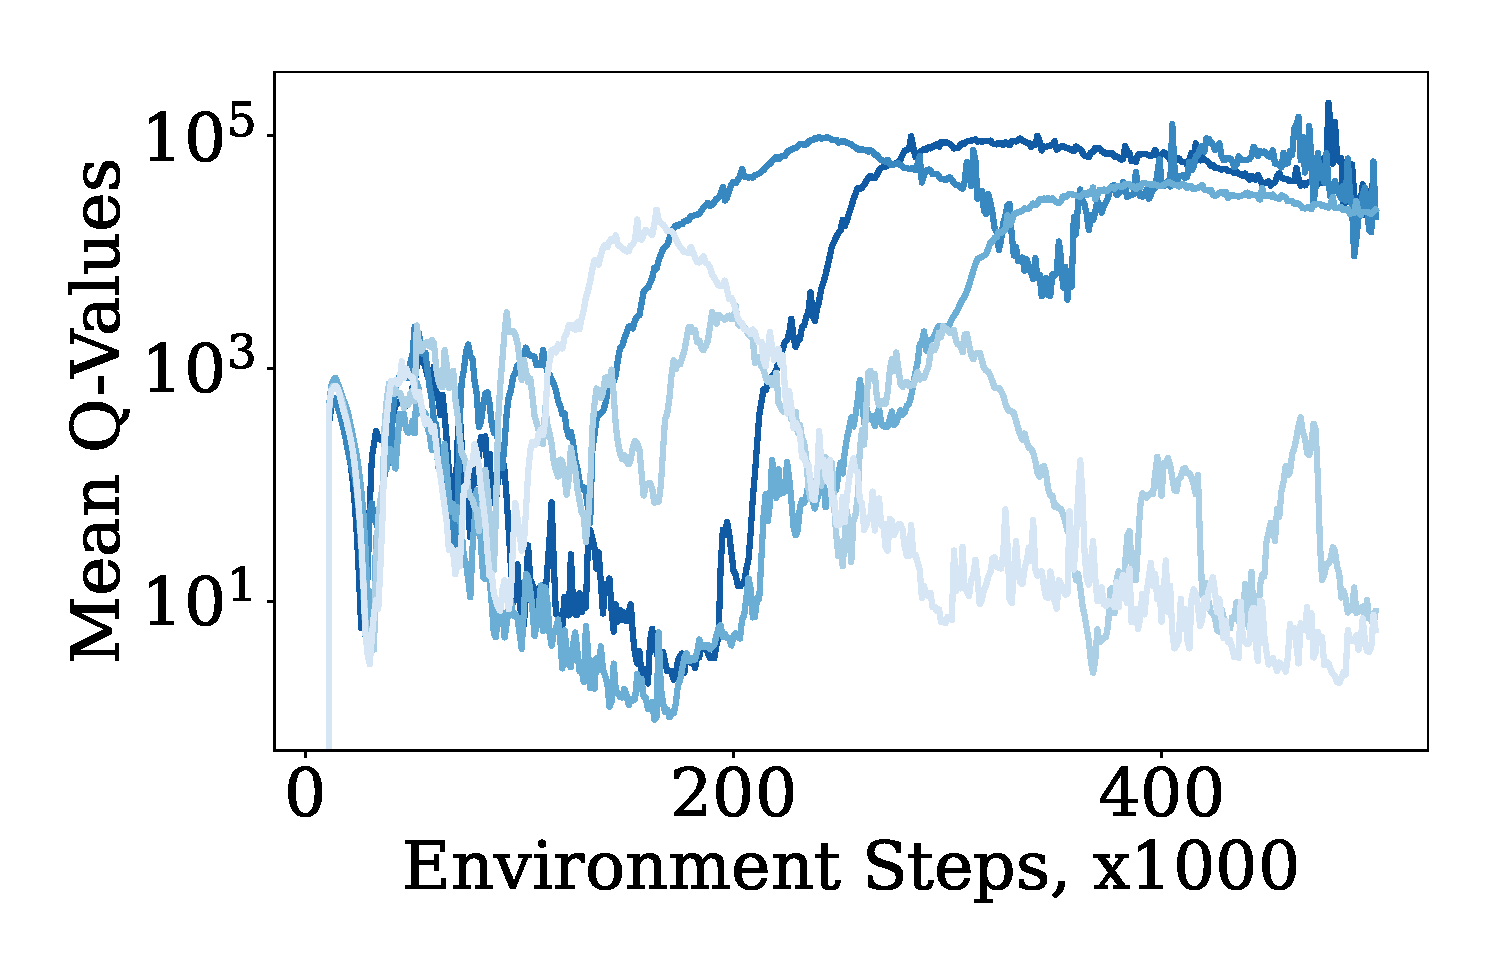
\includegraphics[width=4cm, trim=1cm 1cm 1cm 1cm ,clip]{figures/dissecting/priming/humanoid_Q.pdf}\vspace{-8pt}
    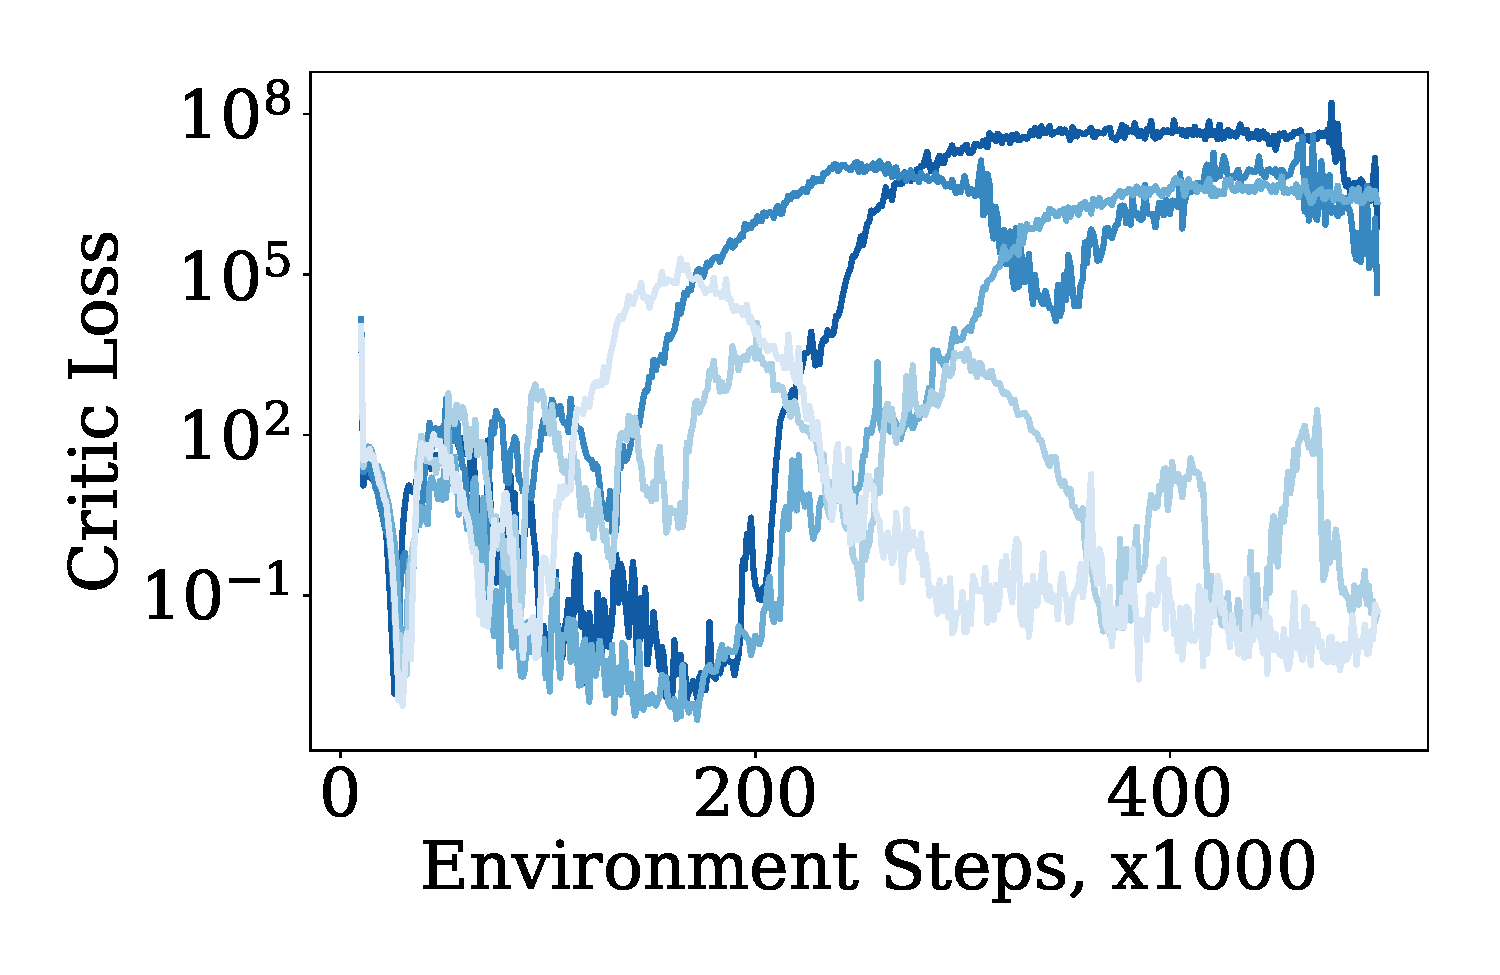
\includegraphics[width=4cm, trim=1cm 1cm 1cm 1cm ,clip]{figures/dissecting/priming/humanoid_loss.pdf}
    \caption{In-distribution Q-values and critic loss of five SAC seeds on the humanoid-run task using $\mathrm{UTD}=32$. Values diverge at arbitrary time-points, not only during the beginning. Loss mirrors Q-value divergence.}
    \label{fig:humanoid_failure}
  \end{minipage}
  \vspace{-15pt}
\end{wrapfigure}
amount of experience but rather one of state-action space coverage. Note that the reported Q-values have been measured on the observed training data, not on any out-of-distribution state-action pairs. 
The respective critic losses become very large. All this points toward a failure to fit Q-values. This behavior does not align with our common understanding of overfitting~\parencite{bishop2006pattern},  challenging the hypothesis that high-UTD learning fails merely due to large validation error~\parencite{li2023efficient}.

\section{Towards high-UTD optimization without resetting} \label{sec:method}

Regularization techniques such as those in Section~\ref{sec:regularization} can fail to alleviate divergence as they tend to operate across the whole network and lower the weights everywhere even if higher values are actually indicated by the data. They also require costly hyperparameter tuning. Thus, we turn towards network architecture changes to the commonly used MLPs that have proven useful in overcoming issues such as exploding gradients in other domains~\parencite{ba2016layer, xu2019understanding}. 

\subsection{Limiting gradient explosion via unit ball normalization} \label{sec:unitball}

\begin{figure}[t]
\begin{minipage}[t]{.60\textwidth}
% \captionsetup[subfigure]{font=footnotesize, aboveskip=2pt}
\centering
    \begin{subfigure}[b]{\textwidth}
        \centering
        
\includegraphics[height=0.4cm]{figures/dissecting/priming/priming_norm_return_legend.pdf}
    \end{subfigure}\\%
    \begin{subfigure}[b]{0.5\textwidth}
        \centering
        %\setlength{\fboxsep}{0pt}\fbox{
        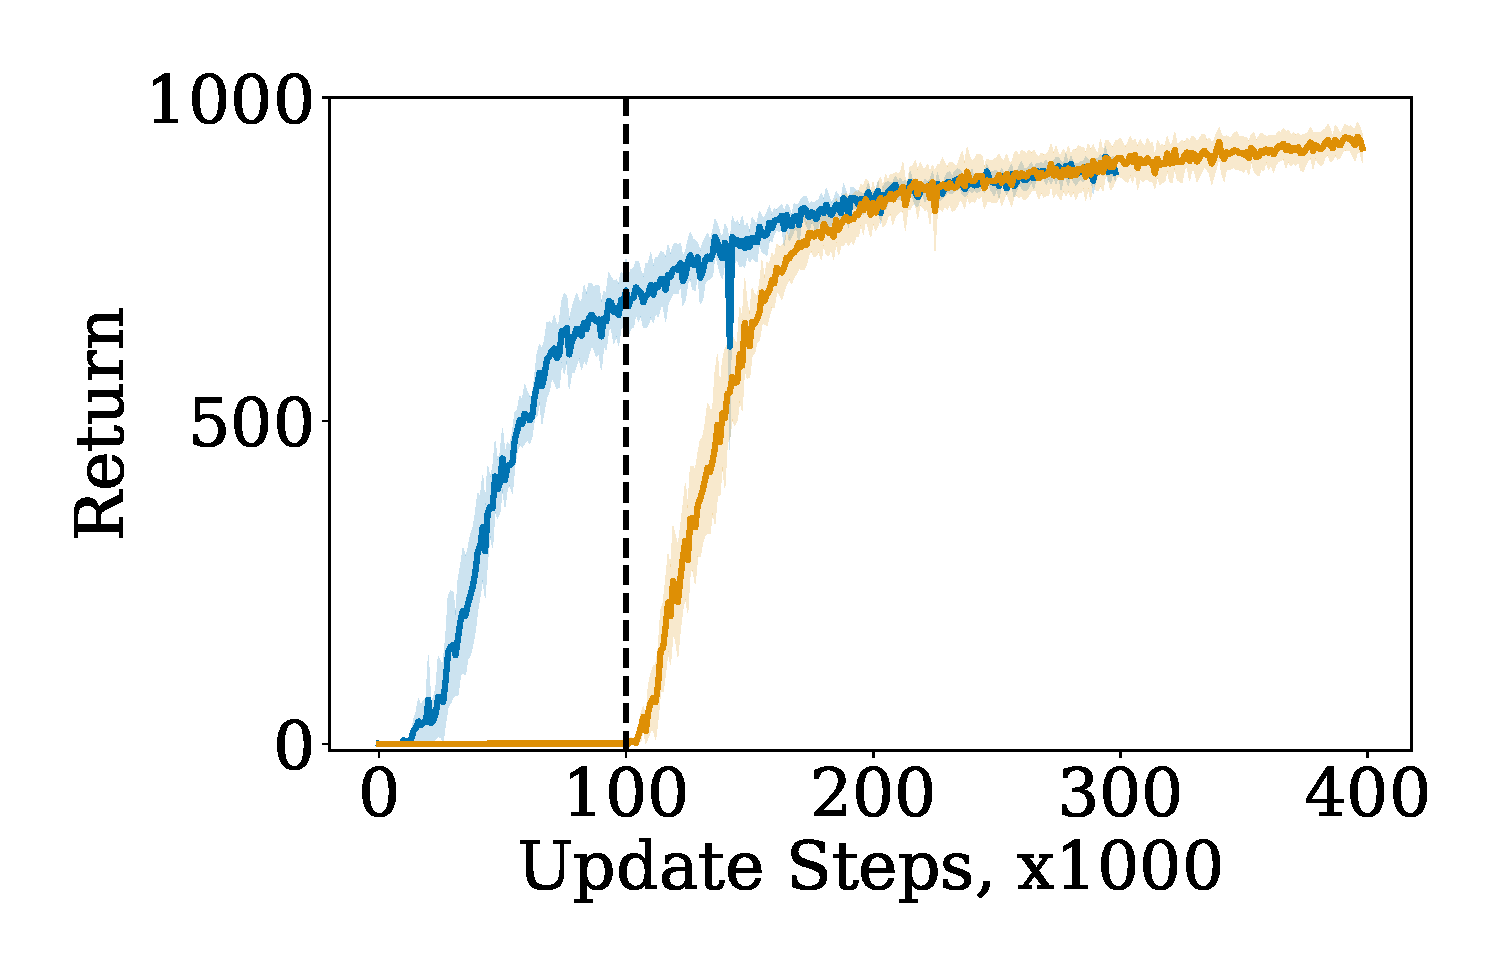
\includegraphics[width=4.8cm,clip,trim=1cm 1cm 1cm 1cm]{figures/dissecting/priming/priming_norm_return.pdf}
        \label{subfig:priming_norm_ret}
    \end{subfigure}%
    \begin{subfigure}[b]{0.5\textwidth}
        \centering
        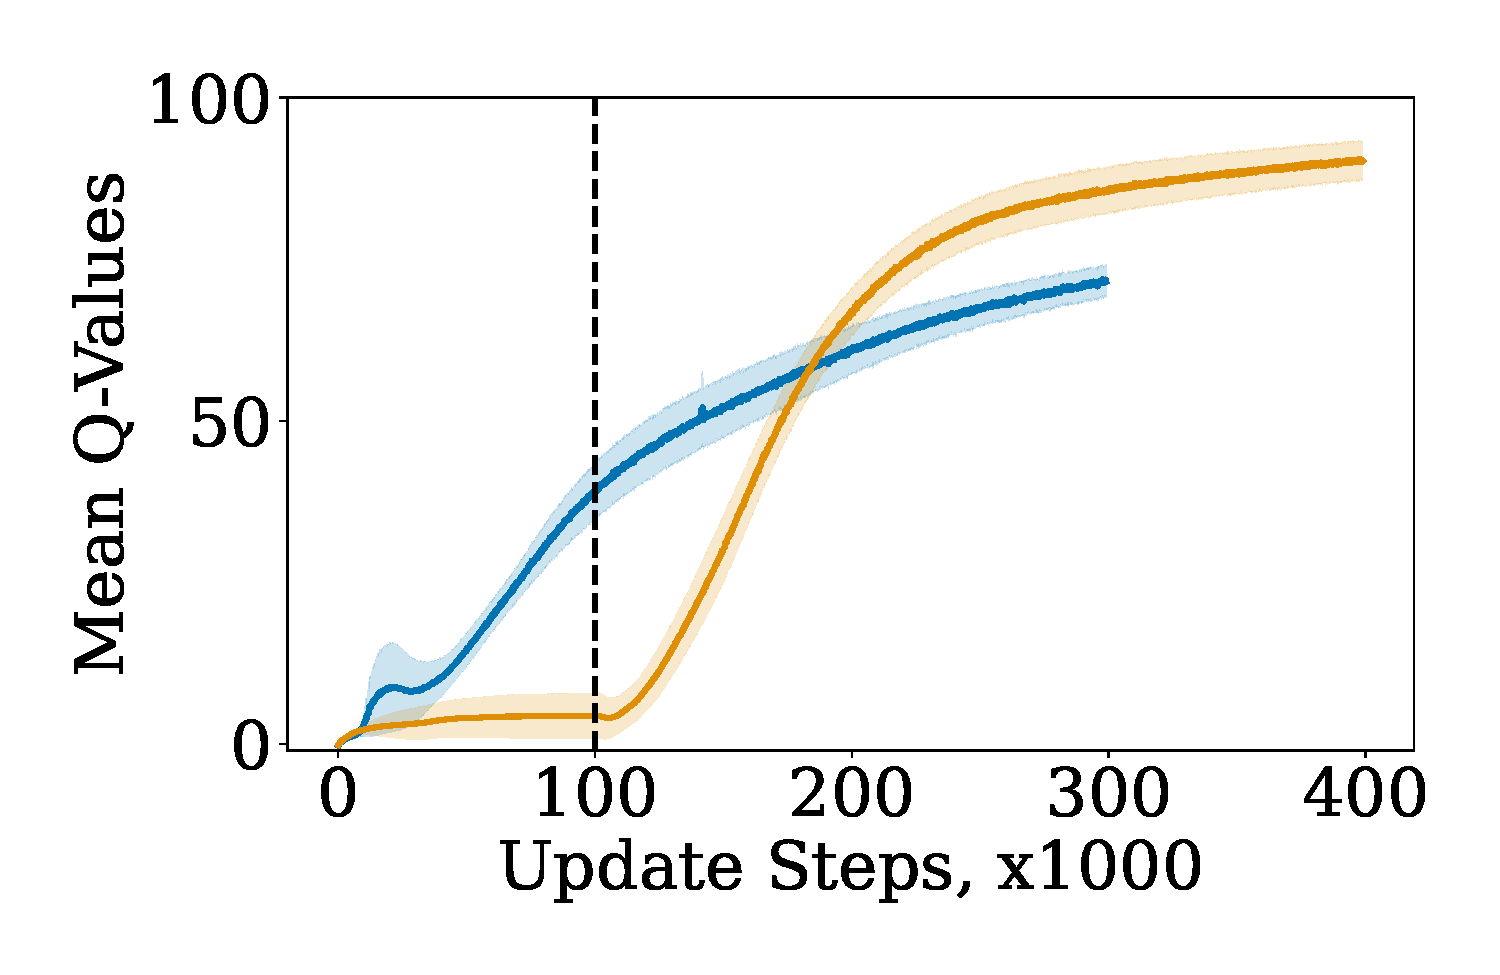
\includegraphics[width=4.8cm,clip,trim=1cm 1cm 1cm 1cm]{figures/dissecting/priming/priming_norm_Q.pdf}
        \label{subfig:priming_norm_Q}
    \end{subfigure}%
    \vspace{-20pt}
    \caption{(Left) Return and (Right) Q-values comparing SGD result and OFN when priming for 100K steps. OFN obtains returns close to that of the well-trained SGD agent and learns an appropriate Q-value scale correctly.}
    \label{fig:priming_norm}
\end{minipage}
\hfill
\begin{minipage}[t]{.36\textwidth}
% \captionsetup[subfigure]{font=footnotesize, aboveskip=2pt}
\centering
    \begin{subfigure}[b]{\textwidth}
        \hspace{15pt}
        \centering
        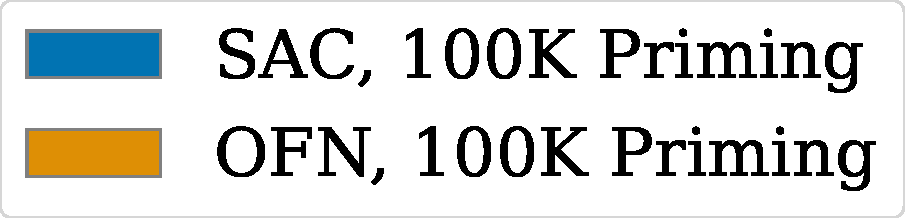
\includegraphics[height=0.8cm]{figures/dissecting/priming/weight_magnitudes_legend.pdf}
    \end{subfigure}
    \\%
    \begin{subfigure}[b]{\textwidth}
        \centering
        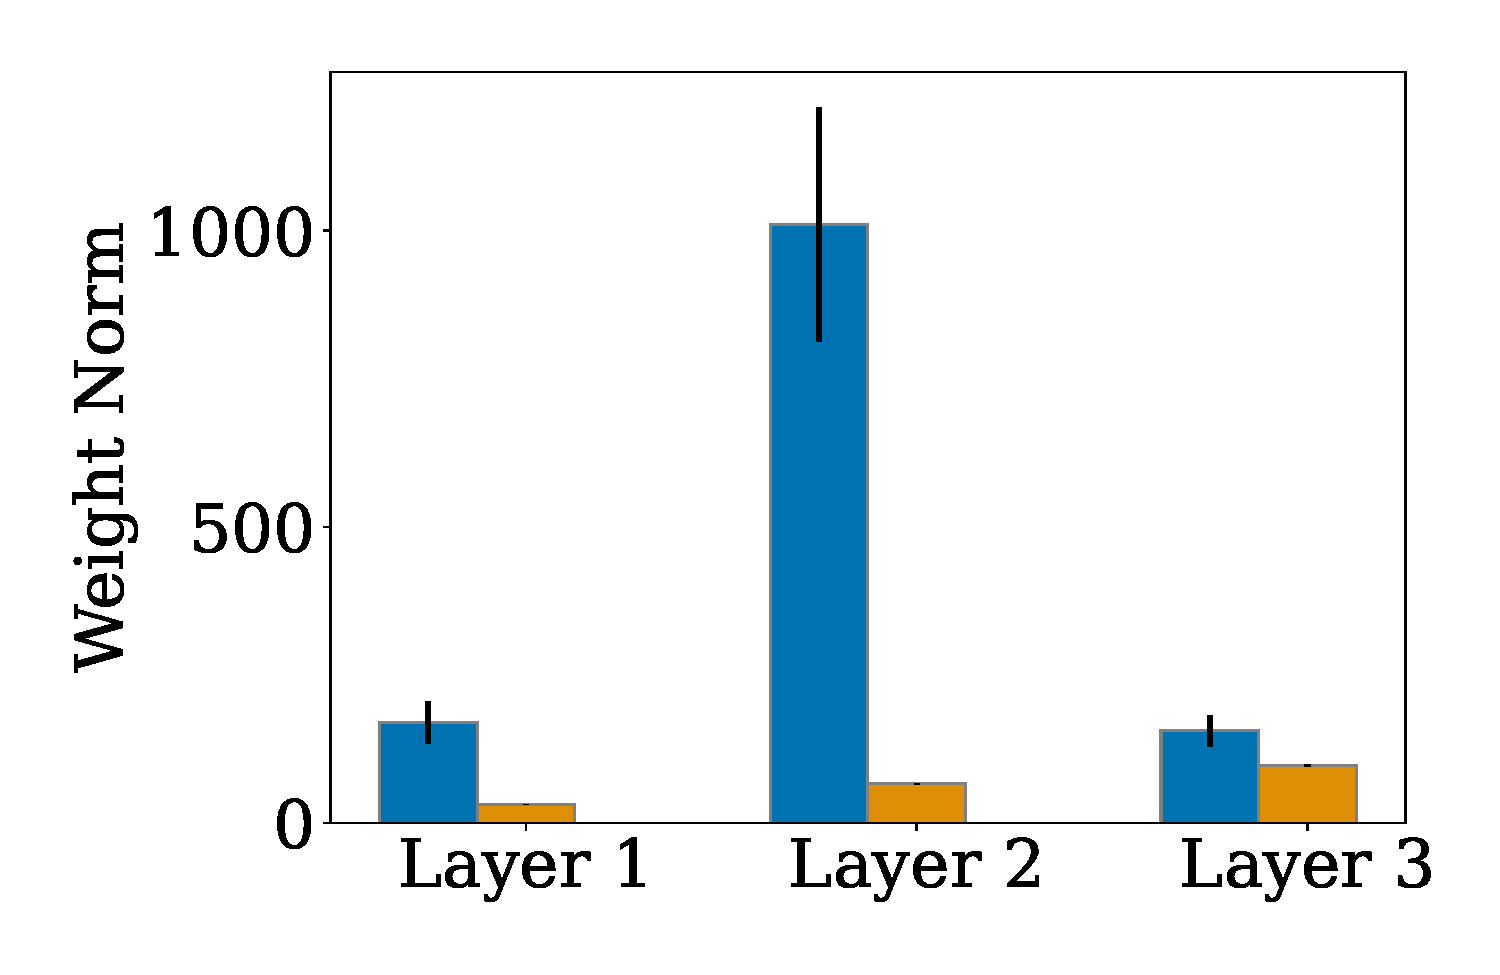
\includegraphics[width=4.6cm,clip,trim=1cm 1cm 1cm 1cm]{figures/dissecting/priming/weight_magnitudes.pdf}
    \end{subfigure}%
    \vspace{-4.5pt}
    \caption{$L_2$ norm of network weights per layer after priming for default and OFN  architectures. OFN leads to smaller weights and significant mass in the last layer.}
    \label{fig:weight_norm}
\end{minipage}
\vspace{-5pt}
\end{figure}

As discussed previously, the prediction of an unknown action might trigger the propagation of a large, harmful gradient. Further, the Q-values of our network ought to grow over time as they more closely approximate those of a good policy. If we predict incorrectly on one of these Q-values, a potentially very large loss is propagated. Gradients are magnified by multiplicative backpropagation via ReLU activations~\parencite{glorot2011deep} as well as momentum from Adam~\parencite{kingma2015adam}. Note that all resulting issues arise in the early network layers. 
We hypothesize that we can address many of these problems by separating the scaling of the Q-values to the appropriate size from the earlier non-linear layers of the network and moving the Q-value scaling to the final linear layer.
%should decouple learning to differentiate Q-values of different actions from scaling the Q-values to the correct magnitude. 
%The former, we want to do in earlier non-linear stages of the network while the latter should solely happen via the last linear transformation.

One contender to achieve the value decoupling described in the previous paragraph is layer normalization~\parencite{ba2016layer}, but one would have to disable scaling factors used in common implementations. Still, standard layer normalization would not guarantee small features everywhere. Instead, we use a stronger constraint and project the output features of the critic encoder onto the unit ball using the function
$f(\mathbf{x}) = \frac{\mathbf{x} }{\|\mathbf{x}\|_2}$~\parencite{zhang2019root}, 
where $\|\cdot\|_2$ denotes the L$^2$ vector norm and $\mathbf{x}$ is the output of our encoder $\phi(s, a)$. This ensures that all values are strictly between $0$ and $1$ and the gradients will be tangent to the unit sphere. Note that this function's gradient is not necessarily bounded to ensure low gradient propagation (see Appendix~\ref{app:unitnorm}), but we argue that if large values are never created in the early layers, gradient explosion will not occur. The unit ball has previously been used to mitigate large action prediction in the actor~\parencite{wang2020striving} or to stabilize RL training in general~\parencite{bjorck2022is}. 
For brevity, we will refer to this method as {\em output feature normalization} (OFN). We solely apply OFN to the critic, unlike~\textcite{wang2020striving}, since our goal is to mitigate value divergence. OFN is very simple and requires only a one-line change in implementation.

% We note the simplicity of the approach as it essentially requires a one-line change in implementation.

% A common technique for normalization of intermediate embeddings is Layer normzliation....
% However, here we make a crucial design choice. Common implementations of layer normalization are implemented via the following rule
% \begin{equation*}
%     l
% \end{equation*}
% where... . We need to ensure that scaling cannot be propagated into our earlier layers and need to disable the learnable parameters of this normalizer. We ablate this choice in Appendix~\ref{todo}


\subsection{Evaluating feature output normalization during priming} \label{sec:evalmethod}

To test the efficacy of the OFN-based approach, we repeat the priming experiment in Figure~\ref{fig:priming_norm}.
We find that OFN achieves high reward and most distinctly, Q-value divergence during priming is fully mitigated. 
Note also that we are using a discount factor of $\gamma = 0.99$, returns are collected over 1,000 timesteps and rewards are in $[0, 1]$. 
We therefore expect the average Q-values to be roughly at $10\%$ of the undiscounted return which seems correct for the OFN network. 
However, more importantly, as shown in Figure~\ref{fig:weight_norm}, most of the Q-value scaling happens in the last layer.

\section{Experimental evaluation}

We evaluate our findings on the commonly used \textsf{dm\_control} suite~\parencite{tunyasuvunakool2020dmcontrol}. All results are averaged over ten random seeds.\footnote{For comparison with TD-MPC2~\parencite{hansen2024tdmpc} we use data provided by their implementation, which only contains three seeds. As the goal is not to rank algorithmic performance but to give intuition about the relative strengths of adapting the network architecture, we believe that this is sufficient in this case.} We report evaluation returns similar to~\textcite{nikishin2022primacy}, which we record every 10,000 environment steps. We compare a standard two-layer MLP with ReLU ~\parencite{nair2010rectified} activations, both with and without resetting, to the same MLP with OFN. %to achieve value clipping. 
The architecture is standard in many reference implementations. Architecture and the resetting protocol are taken from \textcite{doro2023barrier} and hyperparameters are kept without new tuning to ensure comparability of the results. More details can be found in Appendix~\ref{app:impl}.

To understand the efficacy of output normalization on real environments under high UTD ratios, we set out to answer multiple questions that will illuminate RL optimization failures:\\
{\bf Q1:}~Can we maintain learning without resetting neural networks?\\
{\bf Q2:}~Are there other failure modes beside Q-value divergence under high UTD ratios?\\
{\bf Q3:}~When resets alone fall short, can architectural changes enable better high-UTD training?

\subsection{Feature normalization stabilizes high-UTD training} 

\begin{figure}[t]
\begin{minipage}[b]{0.67\textwidth}
% \captionsetup[subfigure]{font=footnotesize, aboveskip=2pt}
\centering
    \begin{subfigure}[b]{\textwidth}
        \centering
        %\setlength{\fboxsep}{0pt}\fbox{
        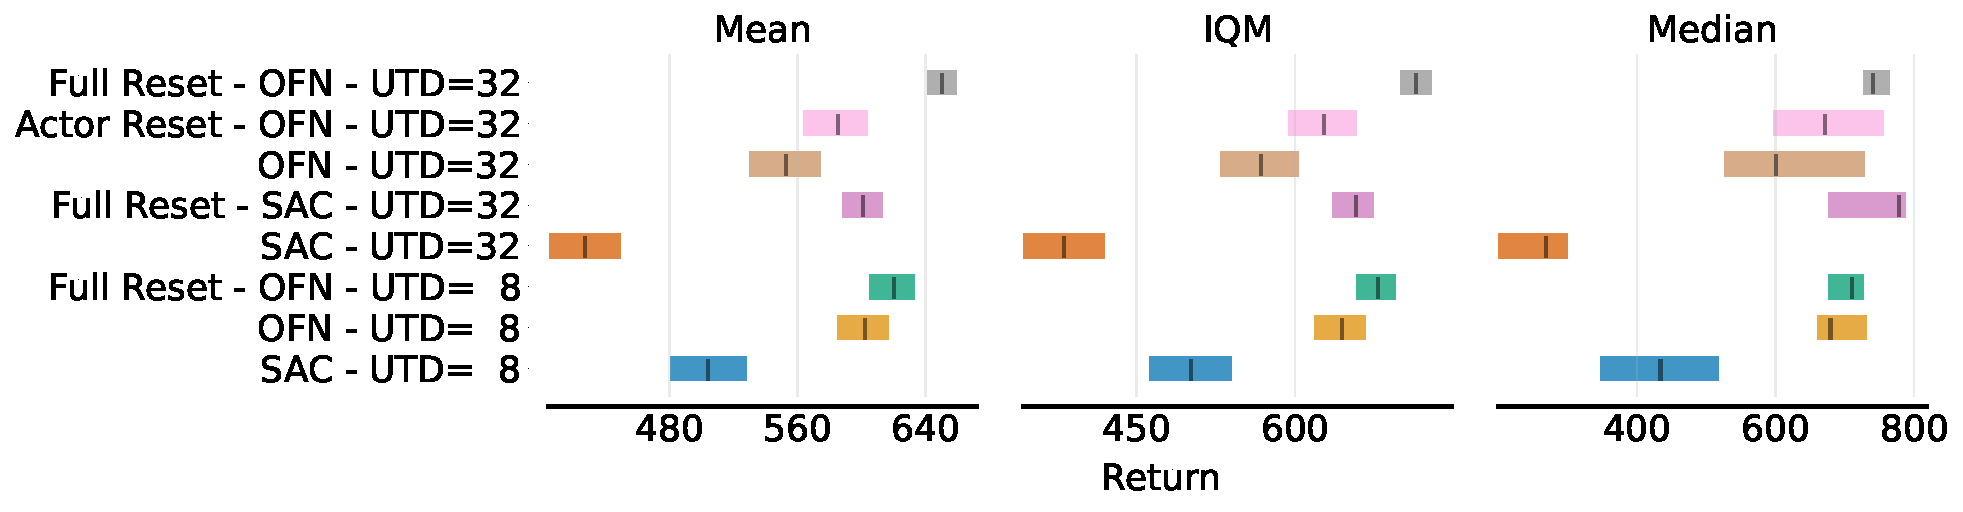
\includegraphics[width=10.2cm,clip,trim=0.3cm 0 0.3cm 0cm]{figures/dissecting/main_exp/all_aggregate_scores.pdf}
        %}
        %\vspace{-1em}
    \end{subfigure}%
    %\vspace{-.8em}
    \caption{Mean, interquartile mean (IQM), and median with $95\%$ bootstrapped confidence intervals of standard SAC and OFN on the DMC15-500k Suite. OFN can maintain high performance even under large UTD. OFN with $\mathrm{UTD} = 8$ achieves comparable performance to standard resetting with $\mathrm{UTD} = 32$ across metrics.}
    \label{fig:aggregate}
\end{minipage}
\hfill
\begin{minipage}[b]{.3\textwidth}
% \captionsetup[subfigure]{font=footnotesize, aboveskip=2pt}
\centering
    % %\vspace{-117pt} 
    % \begin{subfigure}[b]{\textwidth}
    %     %\hspace{15pt}
    %     \centering
    %     %\setlength{\fboxsep}{0pt}\fbox{
    %     
\includegraphics[height=0.8cm]{figures/dissecting/main_exp/hopper_hop_legend.pdf}
    %     %}
    % \end{subfigure}
    % \\%
    \begin{subfigure}[b]{\textwidth}
        \centering
        %\setlength{\fboxsep}{0pt}\fbox{
        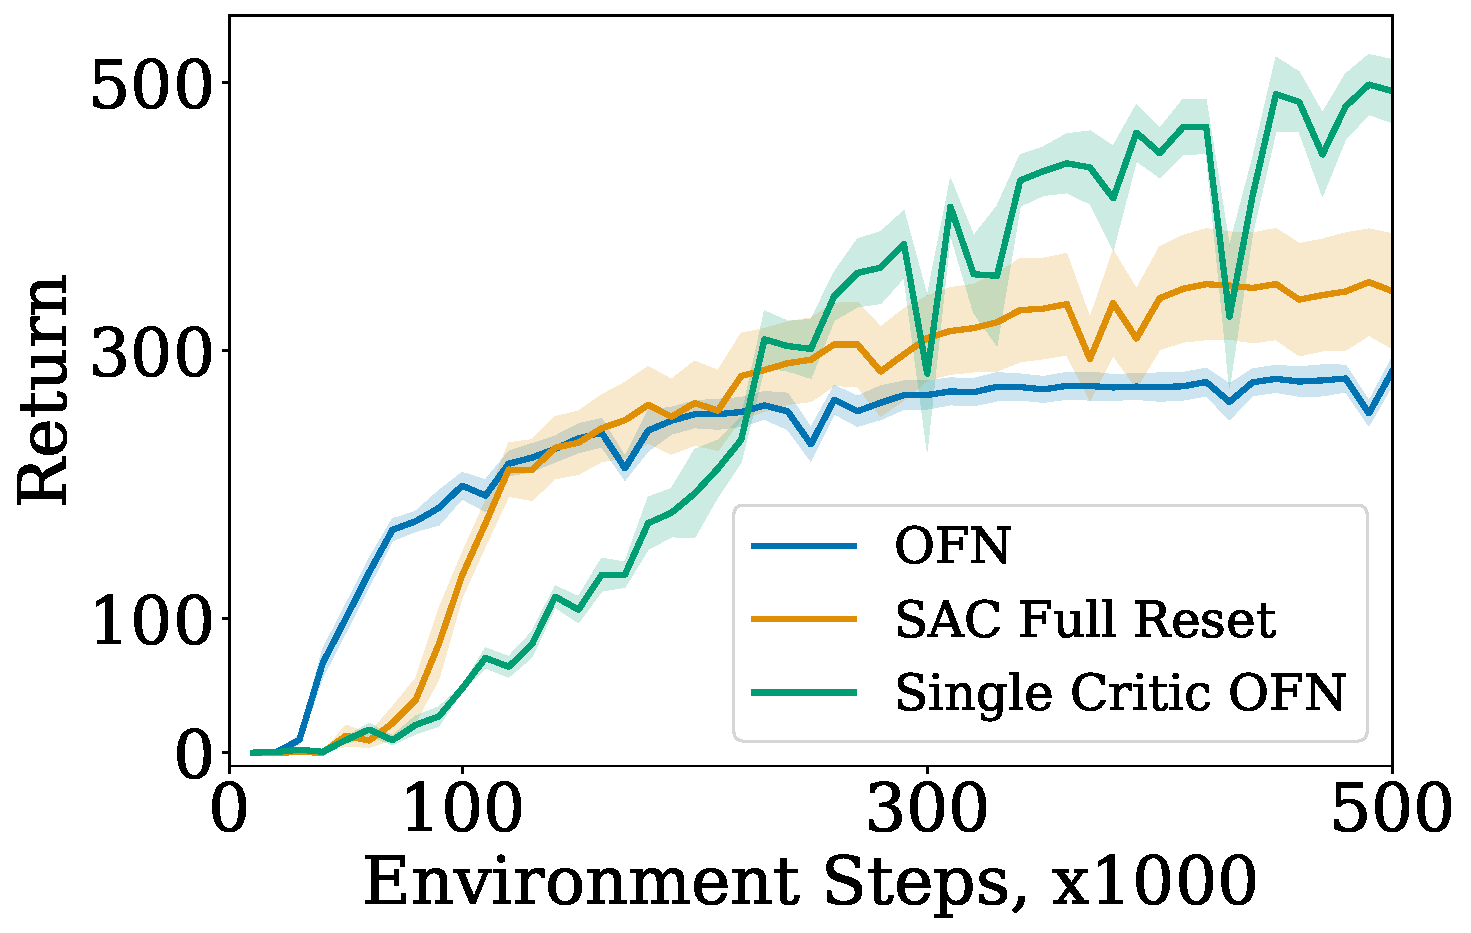
\includegraphics[width=4.25cm,clip,trim=0.3cm 0 0 0]{figures/dissecting/main_exp/hopper_hop_wl.pdf}
         %}
        %\vspace{10pt}
        %\vspace{-1em}
    \end{subfigure}%
    %\vspace{-.8em}
    \caption{Mean return of single-critic OFN, standard OFN and resetting; $\mathrm{UTD}=32$ on hopper-hop. Shaded regions are standard error.}
    \label{fig:hopper_hop}
\end{minipage}
\vspace{-5pt}
\end{figure}

% \begin{figure}[t!]
% \begin{minipage}[b]{.52\textwidth}
% % \captionsetup[subfigure]{font=footnotesize, aboveskip=2pt}
% \centering
%     \begin{subfigure}[b]{\textwidth}
%         \centering
%         %\setlength{\fboxsep}{0pt}\fbox{
%         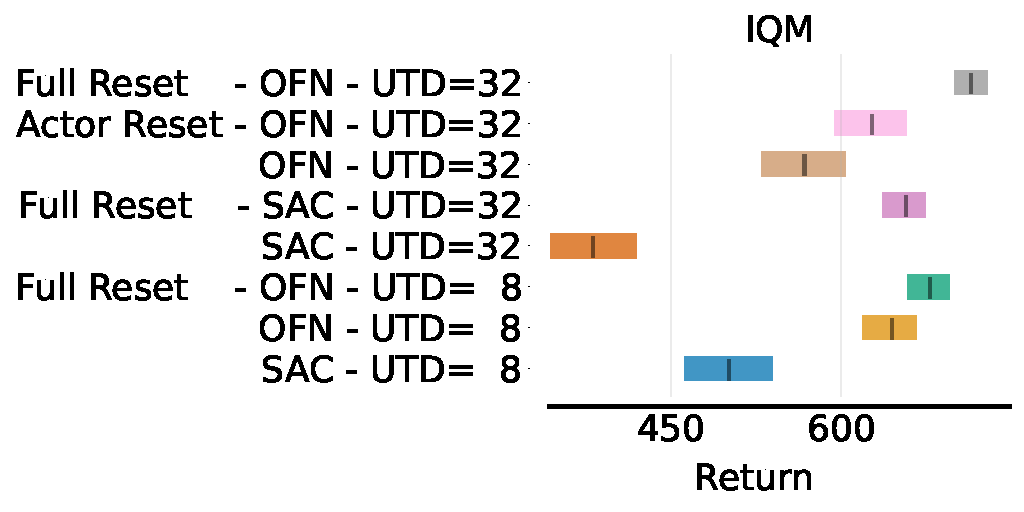
\includegraphics[width=7.3cm,clip,trim=0.3cm 0 0 1cm]{figures/dissecting/main_exp/aggregate_scores.pdf}
%         %}
%     \end{subfigure}%
%     \vspace{-8pt}
%     \caption{Interquartile mean and $95\%$ bootstrapped confidence intervals of high-UTD standard SAC and OFN on the DMC15-500k Suite. OFN can maintain high performance even under large update ratios.}
%     \label{fig:aggregate}
% \end{minipage}
% \hfill
% \begin{minipage}[b]{.45\textwidth}
% % \captionsetup[subfigure]{font=footnotesize, aboveskip=2pt}
% \centering
%     \begin{subfigure}[b]{\textwidth}
%         \centering
%         %\setlength{\fboxsep}{0pt}\fbox{
%         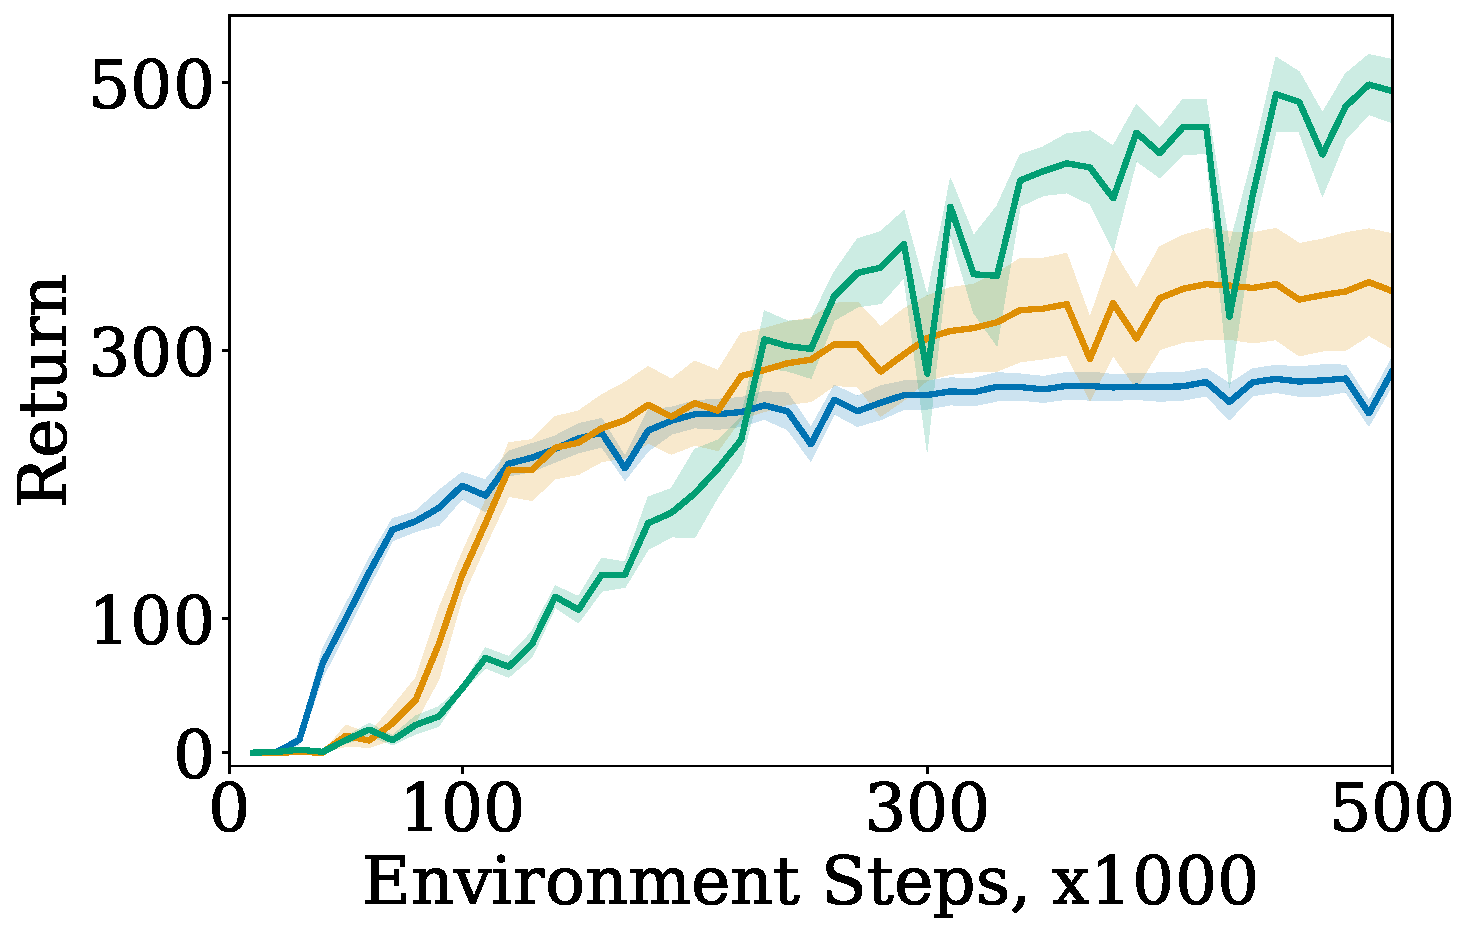
\includegraphics[width=4.6cm,clip,trim=0 0 0 0]{figures/dissecting/main_exp/hopper_hop.pdf}
%         
\includegraphics[height=0.6cm,clip,trim=0cm 0cm 15cm 0cm]{figures/dissecting/main_exp/hopper_hop_legend.pdf}
%         %}
%         \vspace{-8pt}
%     \end{subfigure}%
%     \caption{Single-critic OFN versus standard OFN and standard resetting with $\mathrm{UTD}=32$ on the hopper-hop task. With only a single critic, OFN strongly outperforms resetting.}
%     \label{fig:hopper_hop}
% \end{minipage}
% \vspace{-5pt}
% \end{figure}

% \begin{figure}{r}{0.5\textwidth}
%     \vspace{-12pt}
%     \centering
%     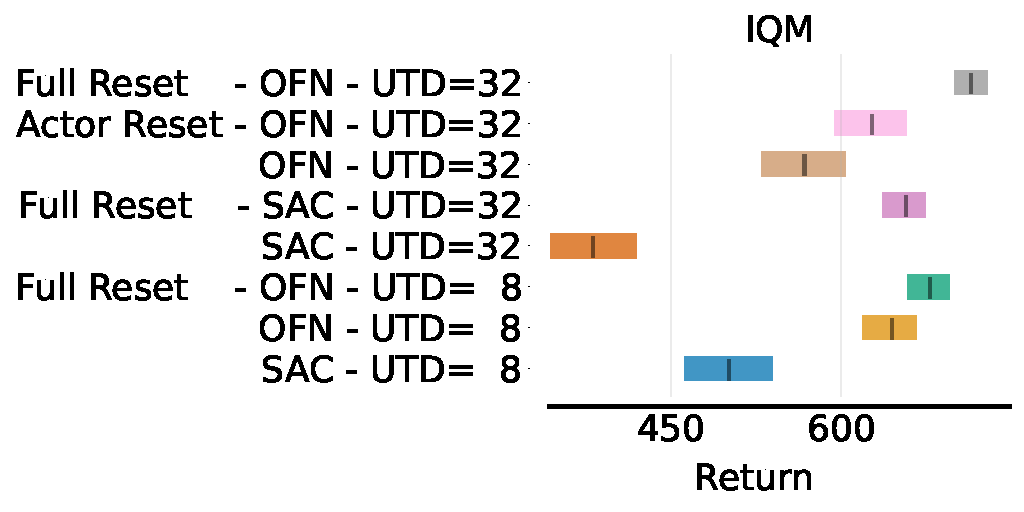
\includegraphics[width=7.3cm, trim={0.3cm 0.3cm 0.3cm 0}, clip]{figures/dissecting/main_exp/aggregate_scores.pdf} 
%     \caption{IQM}
%     \label{fig:aggregate}
%     \vspace{-5pt}
% \end{figure}

To answer \textbf{Q1}, we compare OFN and SAC with resets on the DMC15-500k benchmark with large update ratios of $8$ and $32$ as proposed by \textcite{nikishin2022primacy} and  \textcite{schwarzer2023bigger}.  We report mean, interquartile mean (IQM) and median as well as $95\%$ bootstrapped confidence intervals aggregated over seeds and tasks,  following~\textcite{agarwal2021deep}. The results are shown in Figure~\ref{fig:aggregate}.

First, we observe that in both cases, $\mathrm{UTD}=8$ and $\mathrm{UTD}=32$, OFN can significantly improve over the non-resetting MLP baseline across all metrics. The value estimates that diverge seem to have been handeled properly (see Appendix~\ref{app:exp_q}); learning is maintained. We note that our approach with $\mathrm{UTD}=8$ achieves mean and IQM performance comparable to that of standard resetting with $\mathrm{UTD}=32$. In median and quantile performance, all $\mathrm{UTD}=32$ overlap, highlighting that outliers contribute to the performance measurement. Note that the overall performance drops slightly for the OFN-based approach when going from $\mathrm{UTD}=8$ to $\mathrm{UTD}=32$. We conjecture that there are other learning problems such as exploration that have not been treated by alleviating value divergence. However, these do not lead to complete failure to learn but rather slightly slower convergence. % \comE{unclear last sentence}

\subsection{Other failure modes: Exploration limitations} \label{sec:otherfailure}

% \begin{wrapfigure}{r}{0.36\textwidth}
%     \vspace{-45pt}
%     \centering
%     \hspace{5pt}
%     
\includegraphics[height=0.7cm]{figures/dissecting/main_exp/hopper_hop_legend.pdf} \\
%     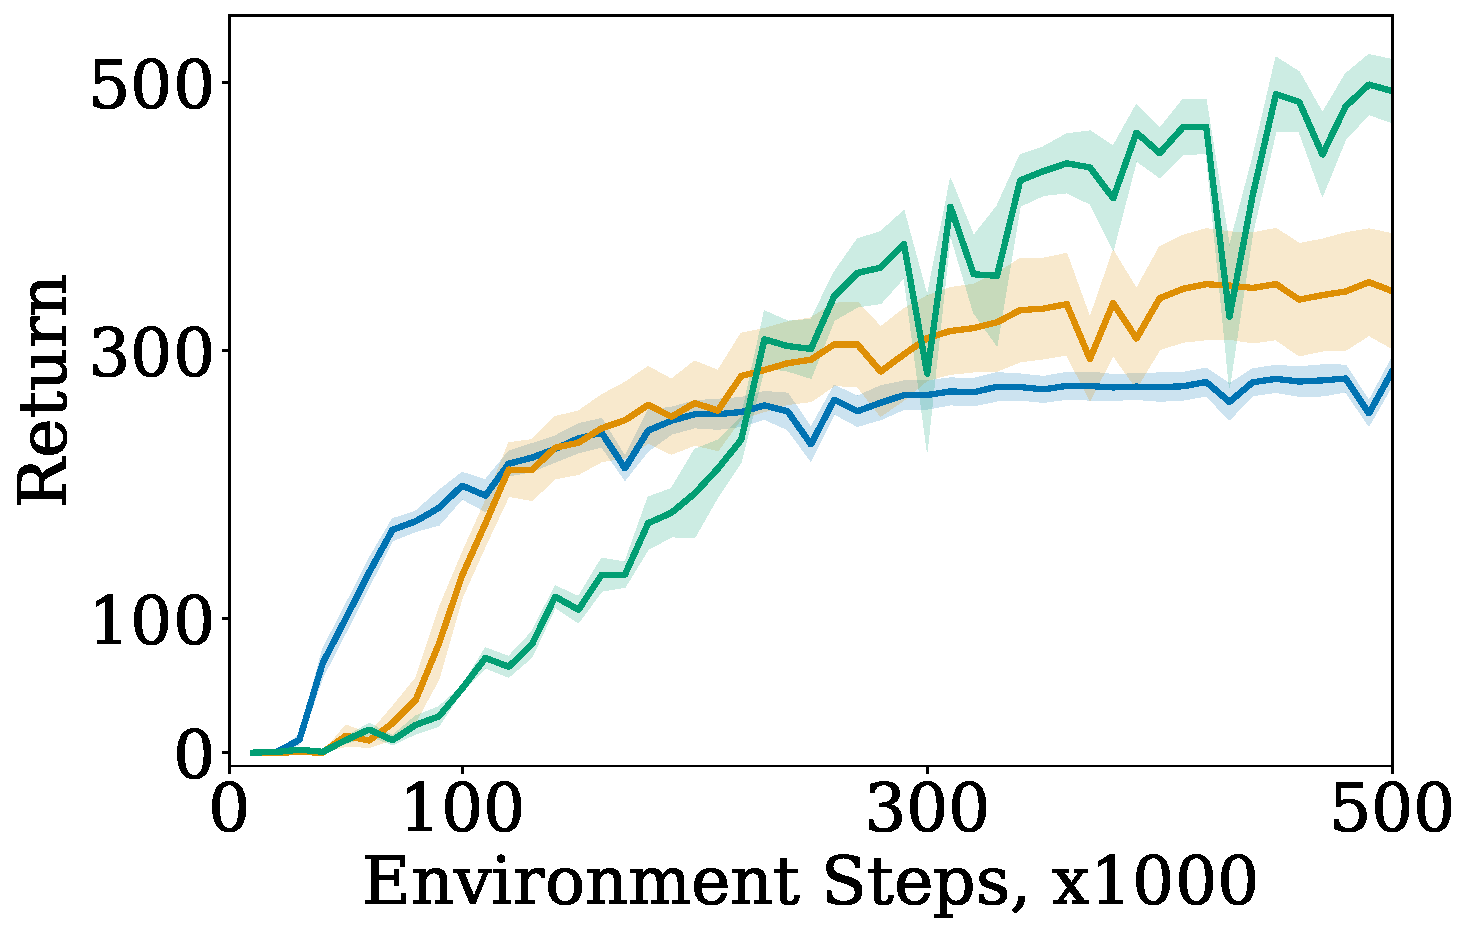
\includegraphics[width=4.8cm, trim={0.3cm 0cm 0.3cm 0.2cm}, clip]{figures/dissecting/main_exp/hopper_hop.pdf} 
%     \vspace{-5pt}
%     \caption{Comparison of single-critic OFN approach to standard OFN and standard resetting with $\mathrm{UTD}=32$ on the hopper-hop task. With only a single critic, OFN strongly outperforms resetting.}
%     \label{fig:hopper}
%     \vspace{-20pt}
% \end{wrapfigure}

To validate the hypothesis of other failures and answer \textbf{Q2}, we run two additional experiments. First, our current focus is on failures of the critic; our proposed mitigation does not address any further failures that might stem from the actor. We defer a more detailed analysis of actor failure cases to future work. Instead, we test the OFN-based architecture again and, for now, simply reset the actor to shed light on the existence of potential additional challenges.
%\comE{Need to better sell that this is ok, and it doesn't violate the premise of the paper of avoiding resetting. Hold the reader's hand}
For comparison, we also run a second experiment in which we reset all learned parameters, including the critic.
% The results are included. \comE{Last sentence is unclear. Included where? Cut, since Figure is mentioned in next sentence?}

The results in Figure~\ref{fig:aggregate} indicate that actor resetting can account for a meaningful portion of OFN's performance decline when going from $\mathrm{UTD}=8$ to $\mathrm{UTD}=32$. The actor-reset results are within variance of the full-resetting standard MLP baseline. Further, we observe that there is still some additional benefit to resetting the critic as well. 
%\comE{Again, need to sell that this is ok.} 
This does not invalidate the premise of our hypothesis, value divergence might not be the \emph{only} cause of problems in the high UTD case. We have provided significant evidence that it is a \emph{major} contributor.
Resetting both networks of OFN with $\mathrm{UTD}=32$  outperforms all other baselines on mean and IQM comparisons. %We set out to study where the improvements induced by critic resets come from.

% \begin{wrapfigure}{r}{0.35\textwidth}
% % \captionsetup[subfigure]{font=footnotesize, aboveskip=2pt}
%   \begin{minipage}{\linewidth}
%     \centering\captionsetup[subfigure]{justification=centering}
%     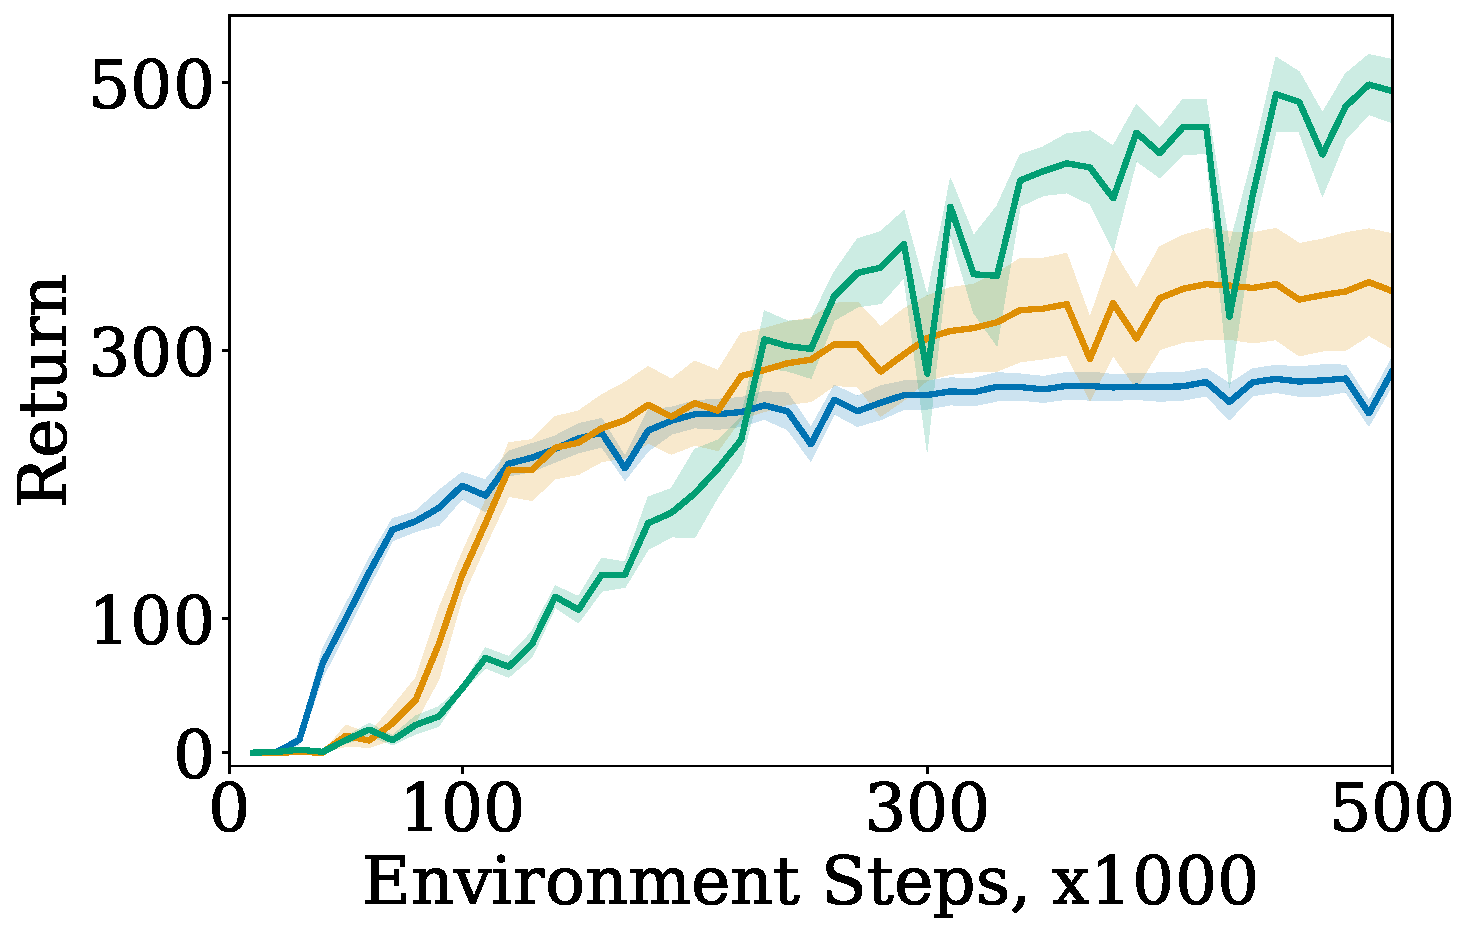
\includegraphics[width=5.4cm, trim=0.3cm 0cm 0cm 0cm ,clip]{figures/dissecting/main_exp/hopper_hop.pdf}
%     \caption{Single-critic OFN versus standard OFN and resetting, with $\mathrm{UTD}=32$ on the hopper-hop task. }
%     \label{fig:hopper_hop}
%   \end{minipage}
%   \vspace{-8pt}
% \end{wrapfigure}

% \begin{wrapfigure}{r}{0.35\textwidth}
%     \begin{minipage}
%     % \captionsetup[subfigure]{font=footnotesize, aboveskip=2pt}
%         % %\vspace{-117pt} 
%         % \begin{subfigure}[b]{\textwidth}
%         %     %\hspace{15pt}
%         %     \centering
%         %     %\setlength{\fboxsep}{0pt}\fbox{
%         %     
\includegraphics[height=0.8cm]{figures/dissecting/main_exp/hopper_hop_legend.pdf}
%         %     %}
%         % \end{subfigure}
%         % \\%
%             \centering
%             \setlength{\fboxsep}{0pt}\fbox{
%             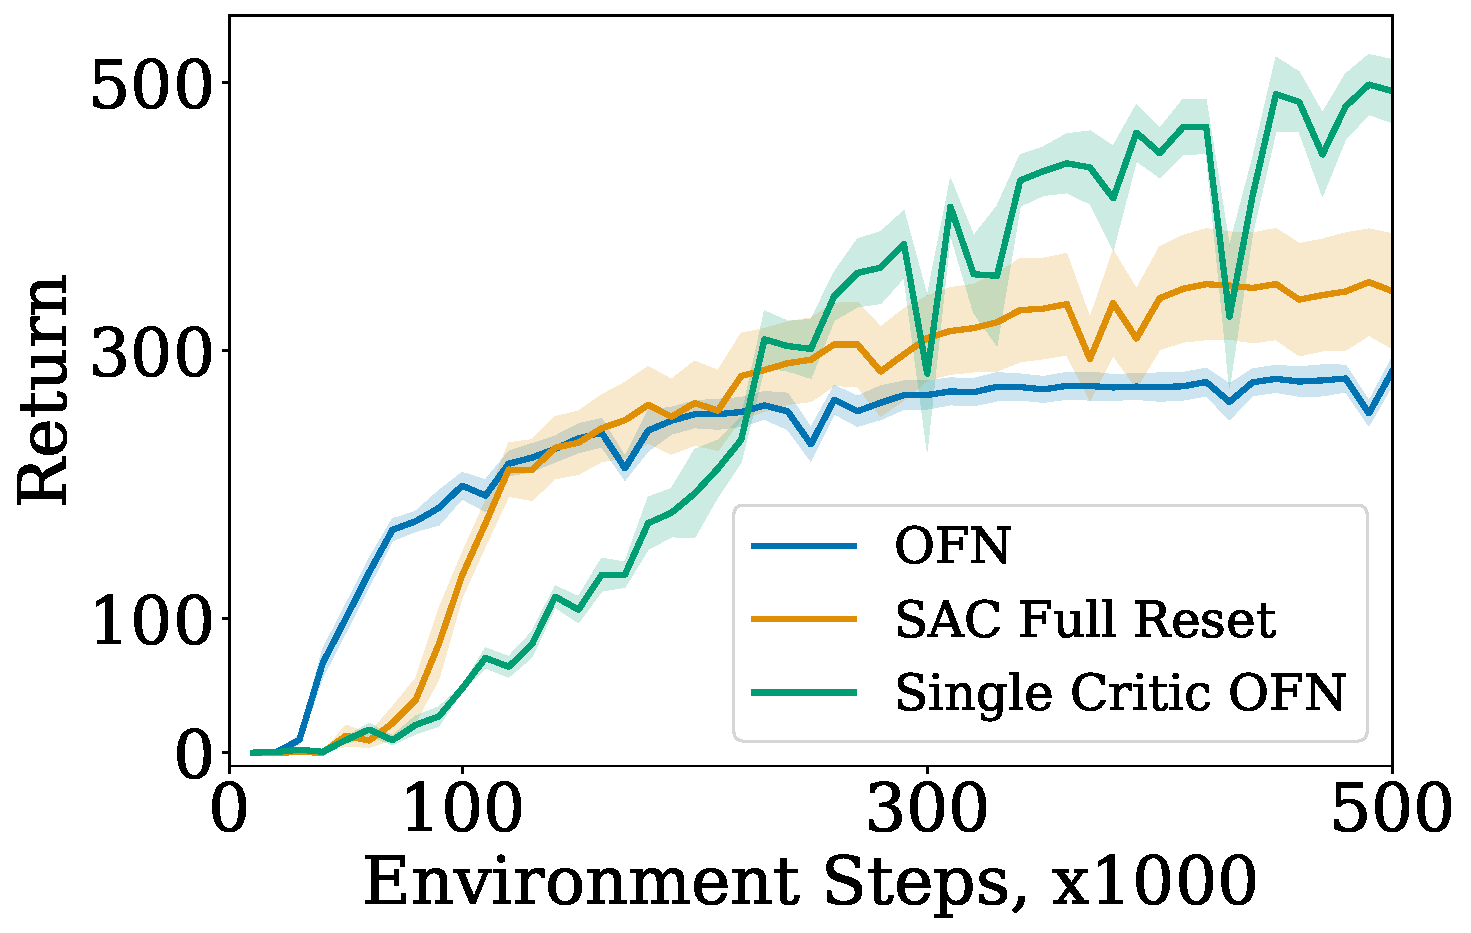
\includegraphics[width=4.25cm,clip,trim=0.3cm 0 0 0]{figures/dissecting/main_exp/hopper_hop_wl.pdf}
%              }
%         \caption{Single-critic OFN versus standard OFN and resetting, with $\mathrm{UTD}=32$ on the hopper-hop task. }
%         \label{fig:hopper_hop}
%     \end{minipage}
% \end{wrapfigure}

To explain the remaining efficacy of critic resets, we examine the hopper-hop environment where standard SAC with resets outperforms OFN. 
%We conjecture that there is an additional exploration benefit inherit to resetting. 
In RL with function approximation, one might not only encounter over-  but also under-estimation~\parencite{wu2020reducing, lan2020maxmin, saglam2021estimation}.
We believe that hopper  is sensitive to pessimism, and periodically resetting the networks might partially and temporarily counteract the inherent pessimism of the dual critic setup.
%Suppose the critic's  overestimation has been handled properly but due to, there are unseen regions of the state-action space whose values are being underestimated. When the network is reset, some regions might now temporarily become overestimated regions, even if we train on the exact same data, which restarts the exploration process.

To obtain evidence for this conjecture, we repeated some experiments with a single critic. As OFN handles divergence it might not require a minimization over two critics~\parencite{fujimoto2018addressing}. We compare OFN using a single critic and $32$ updates per environment step to standard SAC and OFN in Figure~\ref{fig:hopper_hop}. With a single critic, OFN does not get stuck in a local minimum and outperforms full resetting. Note that this is only true in few environments, leading us to believe that the effects of high-update training are MDP-dependent.
In some environments we observe unstable learning with a single critic, which highlights that the bias countered by the double critic optimization and the overestimation from optimization we study are likely orthogonal phenomena that both need to be addressed.
Most likely, there is a difficult trade-off between optimization stability and encouraging sufficient exploration, which is an exciting avenue for future research.

\subsection{Limit-testing feature normalization}

\begin{figure}[t]
% \captionsetup[subfigure]{font=footnotesize, aboveskip=2pt}
\centering
    \begin{subfigure}[b]{0.8\textwidth}
        \centering
        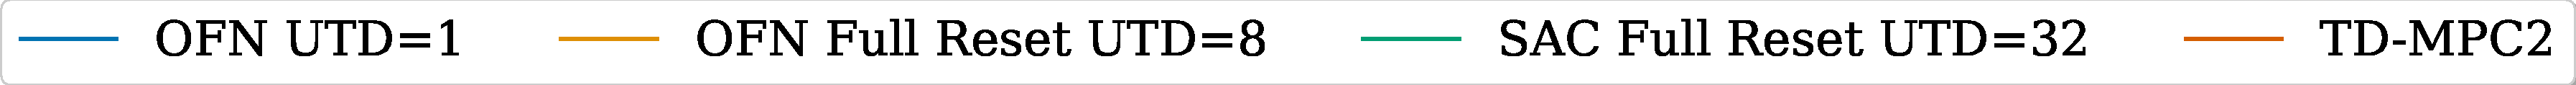
\includegraphics[height=0.4cm]{figures/dissecting/dog_exp/dog_legend.pdf}
    \end{subfigure}\\%
    \hspace{-20pt}
    \begin{subfigure}[t]{0.25\textwidth}
        \centering
        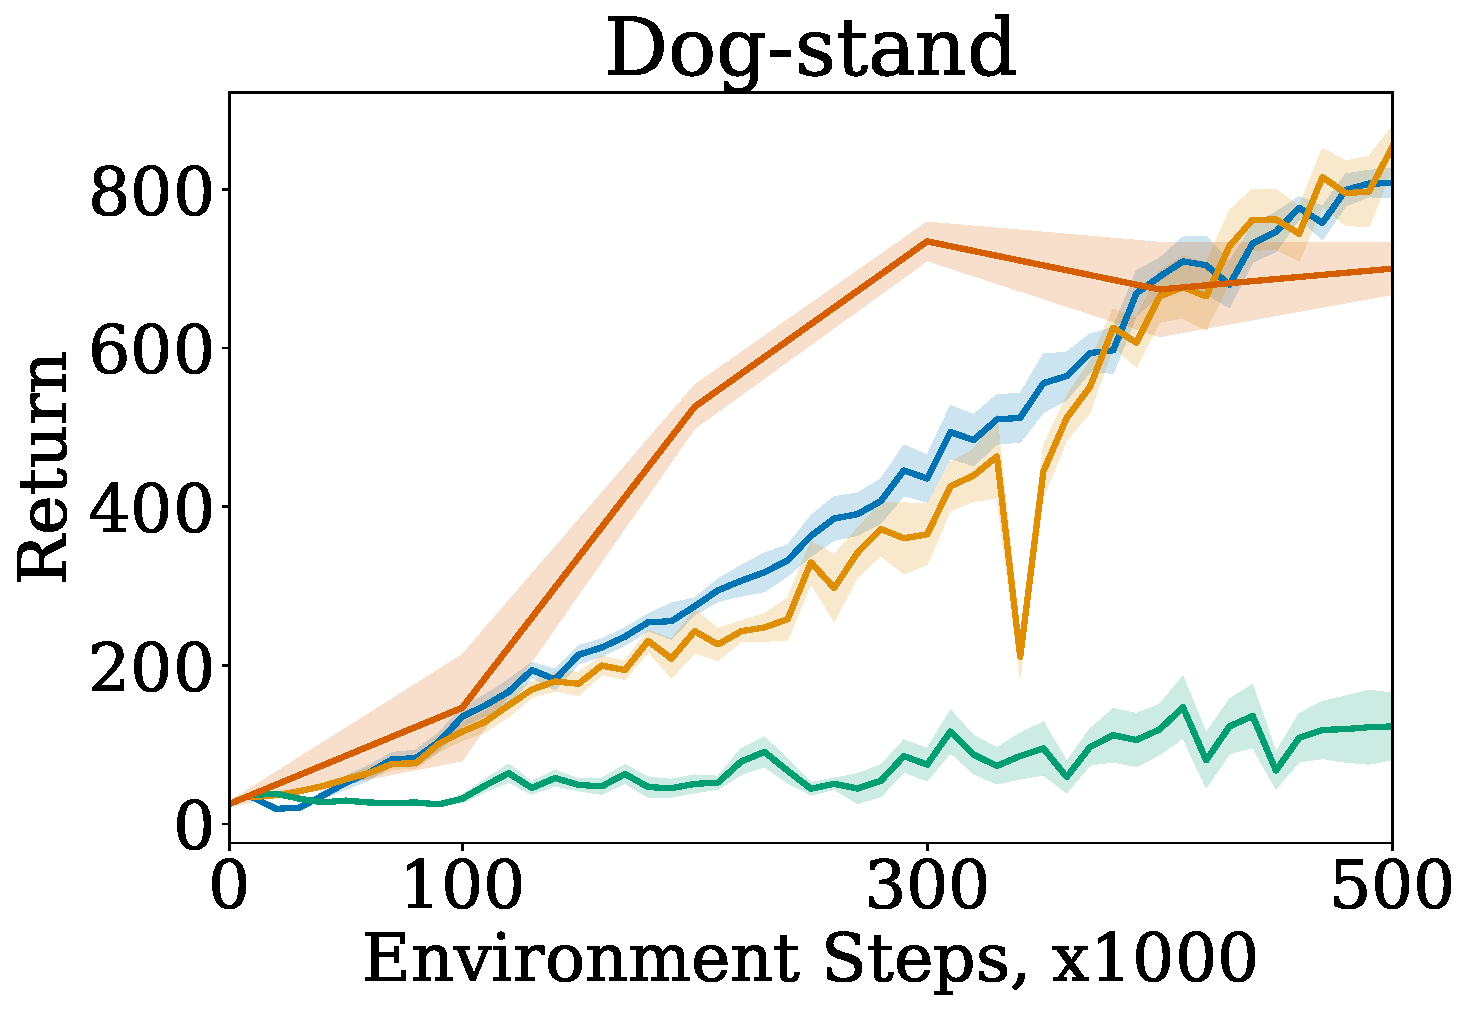
\includegraphics[width=4.cm, trim=0.4 0 0 0 ,clip]{figures/dissecting/dog_exp/dog-stand.pdf}
        \label{subfig:dog_stand}
        \vspace{-12pt}
        % \caption{Dog Stand}
    \end{subfigure}%
    \hspace{5pt}
    \begin{subfigure}[t]{0.25\textwidth}
        \centering
        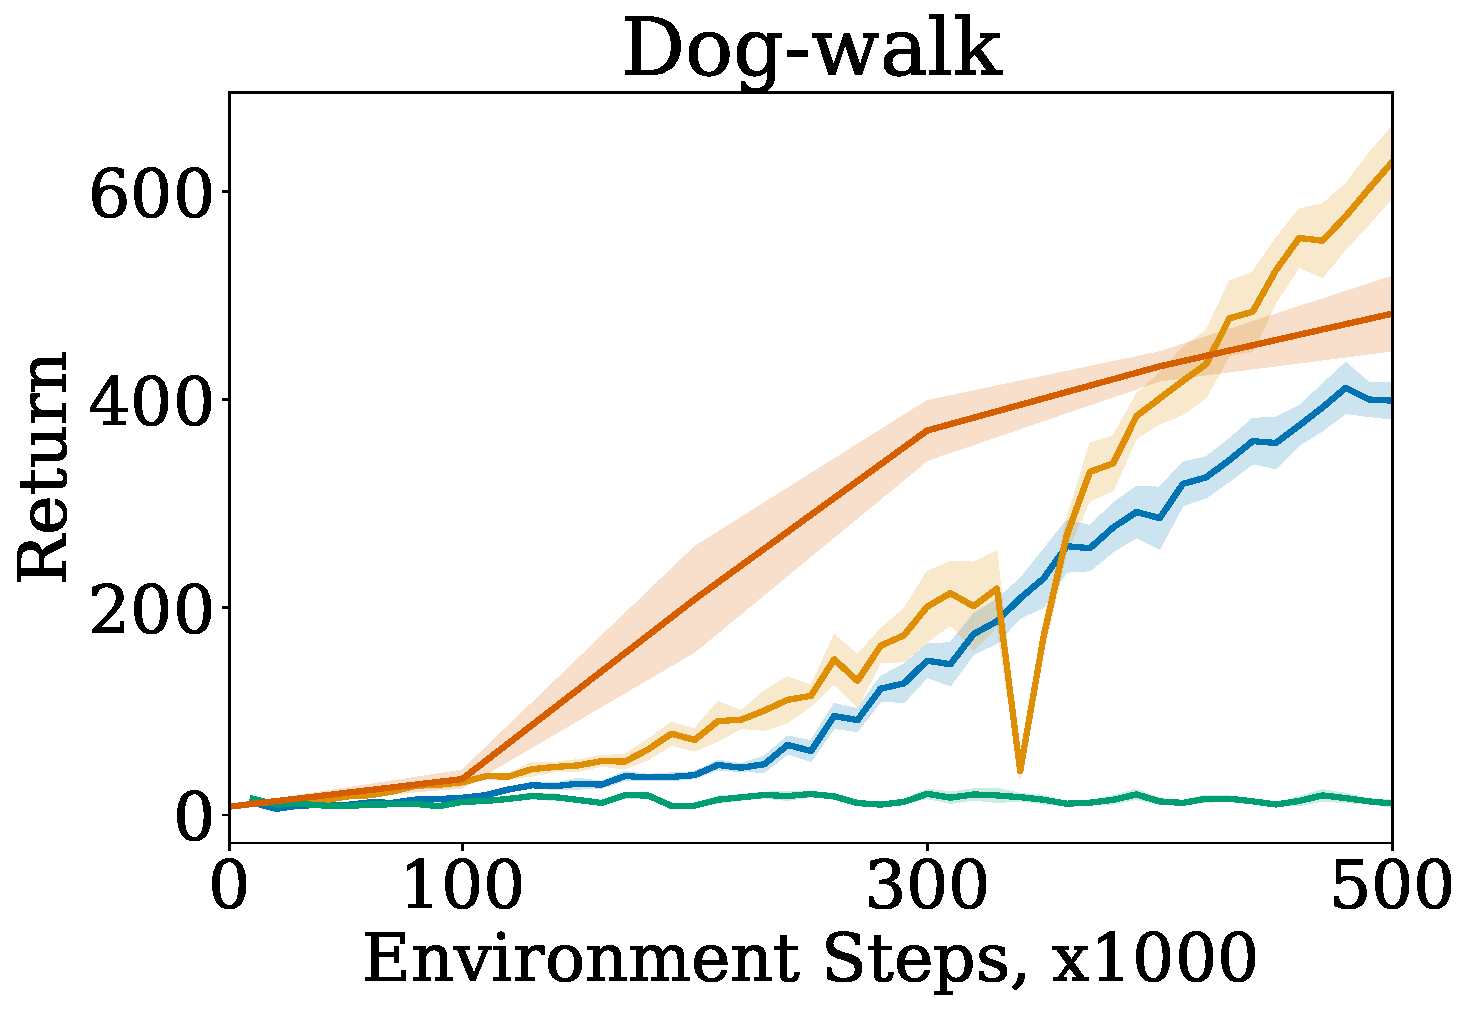
\includegraphics[width=3.7cm, trim=1.2cm 0 0 0 ,clip]{figures/dissecting/dog_exp/dog-walk.pdf}
        \label{subfig:dog_walk}
        % \caption{Dog Walk}
    \end{subfigure}%
    \hspace{-5pt}
    \begin{subfigure}[t]{0.25\textwidth}
    \centering
        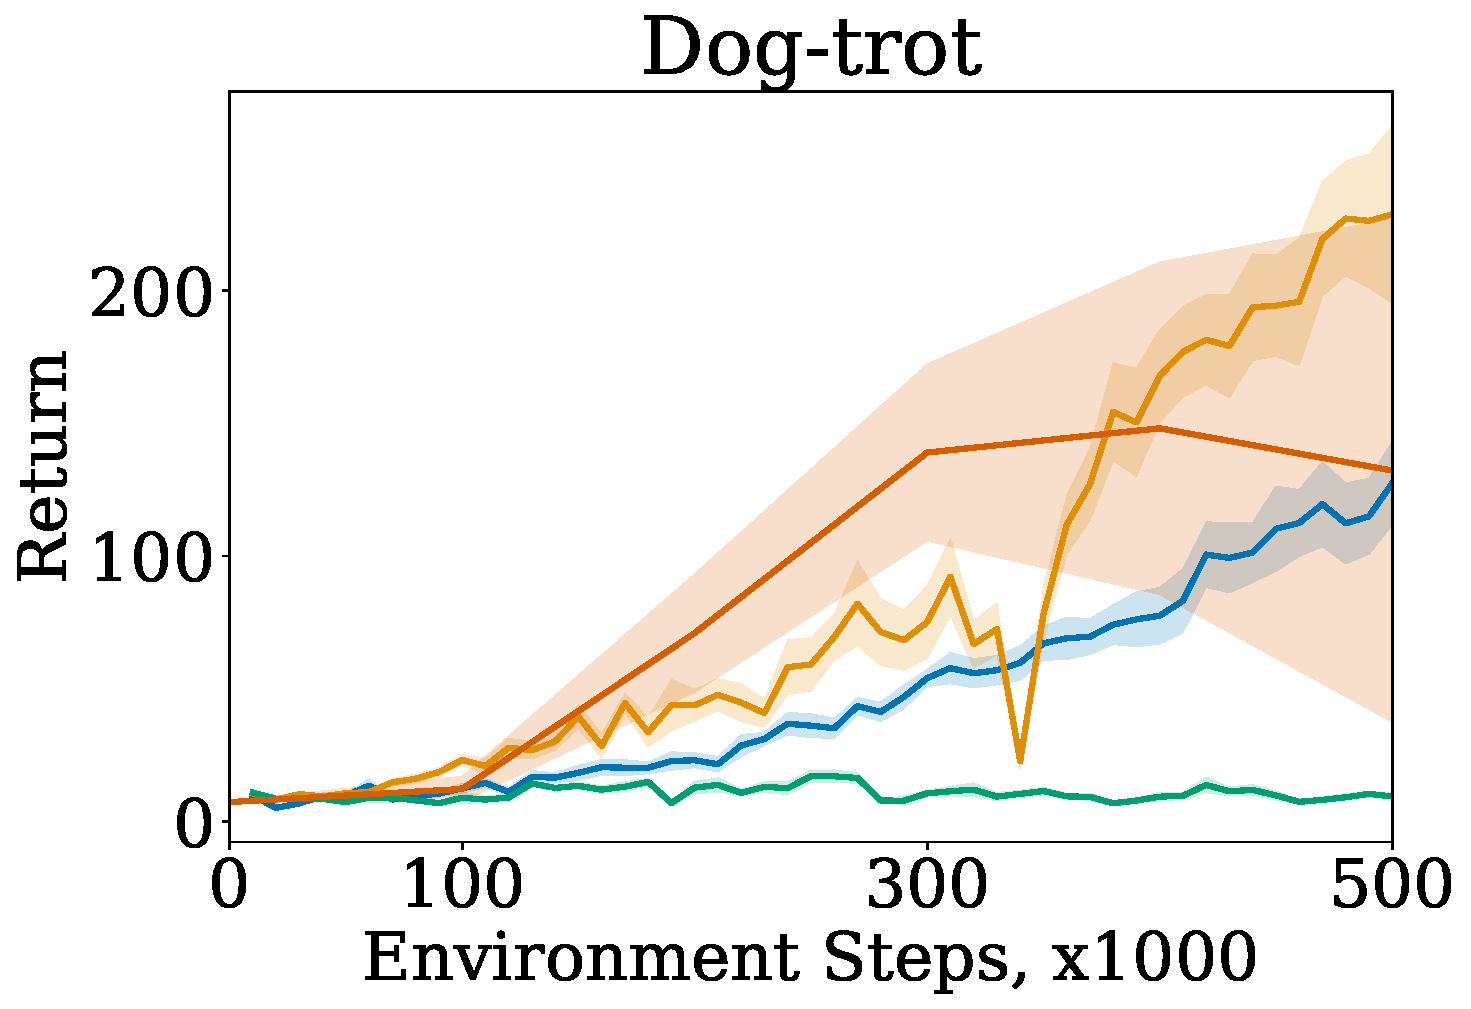
\includegraphics[width=3.7cm, trim=1.2cm 0 0 0 ,clip]{figures/dissecting/dog_exp/dog-trot.pdf}
        \label{subfig:dog_trot}
        % \caption{Dog Trot}
    \end{subfigure}%
    \hspace{-5pt}
    \begin{subfigure}[t]{0.25\textwidth}
        \centering
        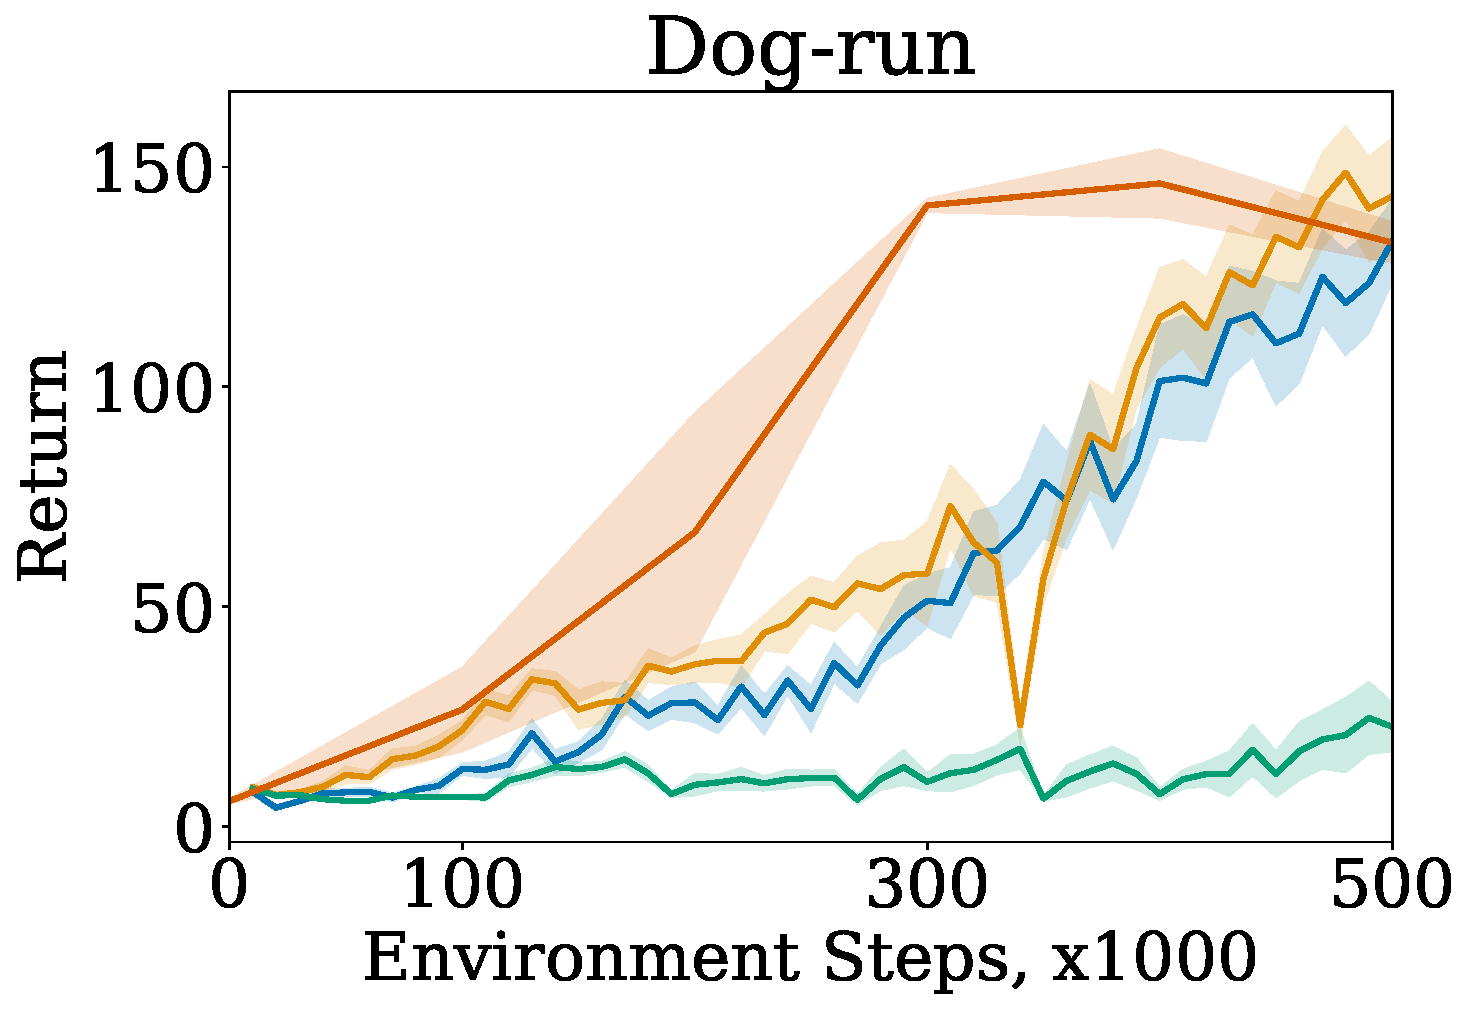
\includegraphics[width=3.7cm, trim=1.2cm 0 0 0 ,clip]{figures/dissecting/dog_exp/dog-run.pdf}
        \label{subfig:dog_run}
        % \caption{RGRDog Run}
    \end{subfigure}%
    \hspace{-20pt}
    % \vspace{-5pt}
    \caption{Mean return on the dog DMC tasks, comparing OFN to SAC with resets and the model-based TD-MPC2. Shaded regions indicate standard error. OFN outperforms SAC with resets, which is unable to learn and OFN with $\mathrm{UTD}=8$ and resetting is competitive with TD-MPC2.}
    \label{fig:all_dog}
\end{figure}

To answer \textbf{Q3}, we move to a set of training environments that is considered exceptionally hard for model-free approaches, namely the dog tasks of the DMC suite. Standard SAC can generally not obtain any reasonable reward and, due to their complex dynamics, these tasks are often tackled using model-based approaches such as TD-MPC2~\parencite{hansen2024tdmpc} with complicated update procedures and carefully tuned network architectures. We evaluate SAC and OFN on the dog tasks and compare against TD-MPC2 in Figure~\ref{fig:all_dog}.

First, observe that resetting without OFN obtains no improvement over a random policy. However, OFN with $\mathrm{UTD}=1$ can already obtain very good performance across all tasks, indicating that a major problem for SAC in these high-dimensional tasks is value divergence. When increasing the update ratio to $8$ and adding resetting, we improve the performance of the OFN agent even further and can match the reported results of the strong model-based TD-MPC2 baseline. 

We have already seen that resetting can take care of multiple optimization failures. However, these experiments also indicate that resetting is not a panacea as it is only effective when the initially learned policy can obtain some reward before being overwritten. 
This seems intuitive since resetting to a policy that cannot gather any useful data should not help. 
These results highlight that the early training dynamics of RL are highly important when it comes to training on complex environments and fitting early data correctly and quickly is crucial for success. 

This also opens up the question why resetting in the humanoid environments in the previous sections can yield success even though very little reward is observed. 
Besides greater divergence due to larger observation spaces in the dog MDPs, we suspect that this might be related to the complexity of exploration.
The ability of a random policy to obtain non-trivial reward and information about the environment has been shown to be a crucial factor in explaining the success of DRL methods in discrete environments~\parencite{laidlaw2023bridging}, and similar phenomena might be in effect here. 

% \comE{\# seeds/trials?  Might be space to add in caption of Fig 9}

% \mh{tie this back to primacy bias, if resetting fixes the primacy bias, it should work here.} \mh{talk about environment specific study and mention bridging paper here} 


\section{Related work}

Our work closely examines previous work on the primacy bias and the related resetting technique \parencite{anderson1992qlearning,nikishin2022primacy,doro2023barrier,schwarzer2023bigger}.
Going beyond, overestimation and feature learning challenges are a widely studied phenomenon in the literature.

{\bf Combatting overestimation}~~
Overestimation in off-policy value function learning is a well-established problem in the RL literature that dates back far before the prime times of deep learning~\parencite{thrun1993issues, precup2001off}. The effects of function approximation error and the effect on variance and bias have been studied~\parencite{pendrith1997estimator, mannor2007bias} as well.
With the rise of deep learning, researchers have tried to address the overestimation bias via algorithmic interventions such as combining multiple Q-learning predictors to achieve underestimation~\parencite{hasselt2010double, hasselt2016deep, zongzhang2017weighted, lan2020maxmin}, using averages over previous Q-values for variance reduction~\parencite{anschel2017averaged}, or general error term correction~\parencite{donghun2013bias, fox2016taming}. In the context of actor-critic methods, the twinned critic minimization approach of \textcite{fujimoto2018addressing} has become a de-facto standard. Most of these approaches are not applicable or break down under very high update ratios.
To regulate the overestimation-pessimism balance more carefully, several authors have attempted to use larger ensembles of independent Q-value estimates \parencite{lee2021sunrise,peer2021ensemble,chen2021randomized,hiraoka2022dropout}. Ensembling ideas were also combined with ideas from distributional RL~\parencite{bellemare2017distributional} to combat overestimation~\parencite{kuznetsov2020controlling}.  Instead of addressing the statistical bias in deep RL, our study focuses on the problems inherent to neural networks and gradient based optimization for value function estimation. Work from offline-to-online RL has demonstrated that standard layer normalization can bound value estimates during offline training and mitigate extrapolation while still allowing for exploration afterwards~\parencite{ball2023efficient}. Layer normalization has subsequently been used to achieve generally strong results in offline RL~\parencite{tarasov2023rebrac}. Our work is also related to a recent contribution using batch-normalization for increased computational efficiency by~\textcite{bhatt2024crossq} who focus on decreasing update ratios rather than increasing them. A concurrent work by~\textcite{nauman2024overestimation} provides a large scale study on different regularization techniques to combat overestimation. This work also demonstrates the efficacy of SAC on the dog tasks when properly regularized but it does not highlight the effects of Q-value divergence from exploding gradients as a key challenge for this set of environments.

{\bf Combating plasticity loss}~~ Another aspect of the primacy bias is the tendency of neural networks to lose their capacity for learning over time~\parencite{igl2021transient}, sometimes termed \emph{plasticity loss}~\parencite{lyle2021understanding, abbas2023loss}. Recent work mitigates plasticity loss using feature rank maximization~\parencite{kumar2021implicit}, regularization~\parencite{lyle2023understanding}, or learning a second copied network~\parencite{nikishin2024deep}. Some of the loss stems from neurons falling dormant over time~\parencite{sokar2023dormant}. A concurrent, closely related work by~\textcite{lyle2024disentangling} disentangles the causes for plasticity loss further. They use layer normalization to prevent some of these causes, which is closely related to our unit ball normalization. Our work differs in that we focus on the setting of high update ratios and use stronger constraints to mitigate value divergence rather than plasticity loss. 

% \textcite{lyle2021understanding} present an alternative regularization to ours which aims to keep the parameters of the network close to initialization.
% Similar to $L_2$ regularization, this introduces a difficult to tune hyperparameter and can prevent learning in the worst case.
% \textcite{nikishin2024deep} show that by learning a second copied network instead of resetting the original network, capacity loss can be prevented.
% However, this method leads to more and more networks over time, as old ones are frozen and no ones initialized, which is inefficient.
% Closely related is the idea of the effective rank of the feature matrix, which captures how strongly correlated certain features are across different samples.
% \textcite{kumar2021implicit} show that this can be regularized explicitly by using an orthogonal loss on the intermediate layers of the network, as this loss requires large correlation matrices, it is much more computationally expensive than simple normalization of the features.

\section{Conclusion and future work}

By dissecting the effects underlying the primacy bias, we have identified a crucial challenge: \emph{value divergence}. 
While the main focus in studying increased Q-value has been on the statistical bias inherent in off-policy sampling, we show that Q-value divergence can arise due to problems inherent to neural network optimization.
This optimization-caused divergence can be mitigated using the unit-ball normalization approach, which shines on the \textsf{dm\_control} benchmark with its simplicity and efficacy. 
With this result, we challenge the assumption that failure to learn in high-UTD settings primarily stems from \emph{overfitting} early data by showing that combating value divergence is competitive with resetting networks. 
This offers a starting point towards explaining the challenges of high-UTD training in more detail and opens the path towards even more performant and sample efficient RL in the future.

However, as our other experiments show, mitigating value overestimation through optimization is not the only problem that plagues high-UTD learning. 
To clearly highlight these possible directions for future work, we provide an extensive discussion of open problems in Appendix~\ref{app:open}. 
Additional problems, such as \emph{exploration failures} or \emph{suboptimal feature learning}, can still exist and need to be resolved to unlock the full potential of high-UTD RL.

    \chapter{Understanding Auxiliary Tasks for Value Function Learning}
\label{chap:understanding}

\begin{quote}
    This chapter is based on \longfullcite{voelcker2024when}.
\end{quote}

\section{Introduction}

As the previous chapter shows, end-to-end critic training can cause problems with learning good intermediate neural network representations.
While regularization can alleviate some of the optimization failures, it only addresses issues of divergence, and does not ensure that relevant information is properly represented in a decision-aware fashion.
To achieve this, we now take a look at \emph{auxiliary tasks} which directly ensure that transition information is well represented in learned features.

Since the emergence of deep learning, techniques for deep supervised learning have been successfully incorporated into reinforcement learning (RL) agents \parencite{dqn,ddpg}.
However, as we have seen, the RL setting contains additional complications such as non-stationary optimization target and the reliance on bootstrapping.
These hurdles generally add instability to the RL training process, and as discussed, \emph{the failure to learn good features} is a central problem in deep RL \parencite{kumar2021implicit,lyle2022understanding,nikishin2022primacy,hussing2024dissecting}.

To mitigate this failure, one common approach is to add auxiliary tasks to the learning objective \parencite{jaderberg2017reinforcement}. 
Popular examples include predicting next state observations \parencite{jaderberg2016reinforcement} and predicting functions of the next state, or latent self-prediction, \parencite{schwarzer2021dataefficient,ni2024bridging}.
To understand the performance of these approaches, recent literature \parencite{tang2022understanding,lelan2023bootstrapped} considers the \emph{learning dynamics} of auxiliary task learning in simple linear surrogate models \parencite{saxe2014exact}.
Findings in the literature show that observation reconstruction should provide better features than latent self-prediction \parencite{behzadian2019fast,tang2022understanding}. 
However, this causes a theory-practice gap as empirical work has found that latent self-prediction outperforms observation reconstruction across many benchmarks \parencite{schwarzer2021dataefficient,ni2024bridging}.
This suggests that the assumptions made in \textcite{behzadian2019fast,tang2022understanding} might not match the setting that is commonly investigated in the empirical literature.

To address this gap, we pose two questions: \emph{(a) How do auxiliary losses behave when combined with a TD loss?} \textcite{tang2022understanding,lelan2022generalization,tang2023towards} have studied the learning dynamics of auxiliary tasks alone, evaluating their performance without addressing the interaction between the auxiliary task and the main goal, to learn a (correct) value function. \emph{(b) How can we describe the behavior of auxiliary losses in the presence of distractions (states and transition dynamics irrelevant for the reward) and observation functions (different ways to measure the underlying state)?} \ac{mdp}  structures like distractions have been hypothesized to lead to differing performance between different auxiliary tasks \parencite{ni2024bridging}, but to our knowledge no theoretical study has been established.


\autoref{sec:understanding:background} we briefly review notation and provide a formal model of the studied representation losses.
In \autoref{sec:understanding:formalism}, we present a formalization of distractions and observation functions. We use the framework of \emph{factored MDPs} \parencite{boutilier2000stochastic} with Kronecker products \parencite{mahadevan2009learning} to represent a common class of distractions. To model observation functions, we use \emph{linear reparametrization} as a tractable way to go beyond one-hot representations. 

In \autoref{sec:understanding:stand_alone_tasks} and \autoref{sec:understanding:auxilliary_tasks} we analyze the features learned with observation prediction and latent self-prediction alone and in combination with TD learning. 
We also show how these stationary features change with the introduction of distractions and observation functions.
From this analysis we find that latent self-prediction is a strong \emph{auxiliary task}, while observation prediction is a strong feature learning method when used \emph{alone}.
The differences are highlighted in \autoref{fig:understanding:losses}.
This bridges one of the biggest gaps between previous analysis of learning dynamics and empirical results.

In \autoref{sec:understanding:empirical} we test the predictions derived from our theoretical framework by evaluating feature learning losses in the MinAtar suite \parencite{young19minatar}\footnote{All code for our experiments is available at \url{https://github.com/adaptive-agents-lab/understanding_auxiliary_tasks}.}.
We design ablations that mirror both our formalization and previous approaches to test distraction robustness in empirical environments. 
The theory partially predicts the performance differences in the test suite, validating that the insights we obtain from the simple linear surrogate models used for analysis are useful for practitioners.
However, as we have an incomplete understanding of the underlying benchmark problems themselves \parencite{voelcker2024can}, more research is needed to fully characterize the interaction of the environment dynamics with the stabilizing auxiliary tasks.

\begin{figure}
    \centering
    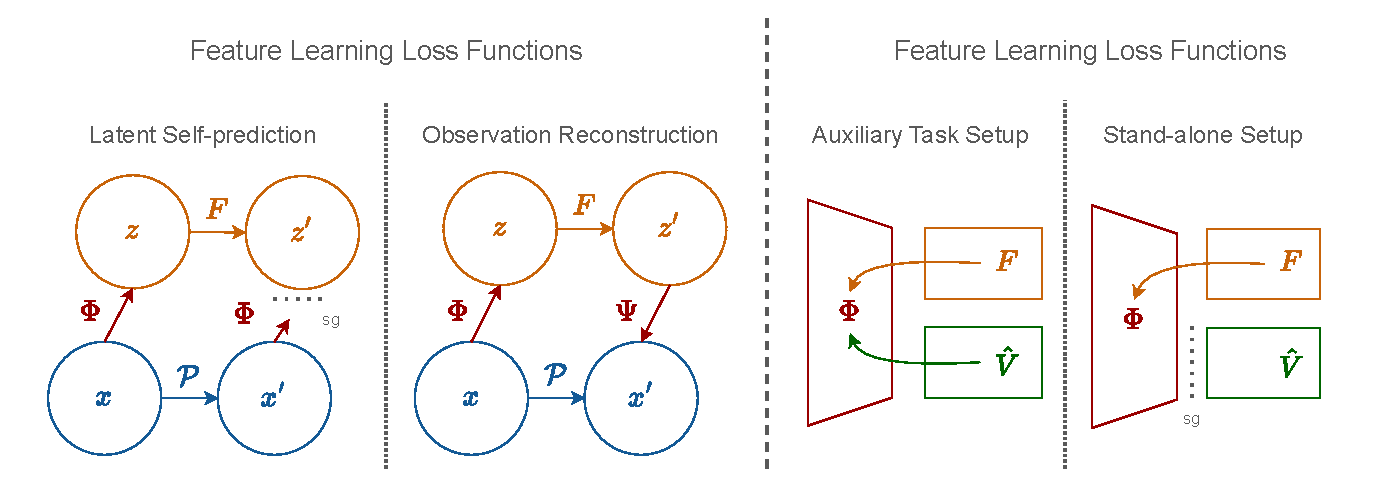
\includegraphics[width=\textwidth]{illustrations/thesis_understanding_overview.pdf}
    \caption{Diagram of the discussed loss functions and use cases. In latent self-prediction, we aim to predict the next state's \emph{features}, computed with an embedding function $\phi(x')$ using the state's features $\phi(x)$ and a latent prediction model $F$. In observation reconstruction, the next state's \emph{ground truth observations} $x'$ are matched via the use of a decoder function $\psi(F(\phi(x)))$. In the \emph{auxiliary task setup}, both the gradients from the feature learning loss and value function learning are propagated to the encoder, while in the \emph{stand-alone scenario}, only the gradients from the feature learning loss are used to update $\Phi$.}
    \label{fig:understanding:losses}
\end{figure}

\section{Mathematical formalism for analysis}
\label{sec:understanding:background}

In this chapter, we will focus on learning in finite state-action problems.
However, our approximations will not be tabular, as discussed in \autoref{chap:background}, but two layer linear networks.
This allows us to discuss the mechanisms underlying representation learning in a tractable setting.
We will generally assume that our states are represented by one-hot vectors.

\subsection{Linear networks as analytical models for training dynamics}

Rigorously analyzing the effect of different loss functions on neural networks is challenging due to non-linearities in the networks, shifting data distributions, and policy updates.
Therefore, we have to resort to studying simplified models to obtain quantitative and qualitative results, and only consider policy evaluation in our analysis.
Studying feature learning dynamics using linear networks was popularized by \textcite{saxe2014exact} and has proven to be a valuable tool to analyze diverse objectives such as TD learning \parencite{tang2023towards,lelan2023bootstrapped}, latent self-prediction \parencite{tian2021understanding,tang2022understanding}, and linear auto-encoders \parencite{pretorius2018learning,bao2020regularized}.

We rewrite the feature learning algorithms using two to three matrices in lieu of more complex functions. 
The embedding function or encoder $\Phi \in \mathbb{R}^{n \times k}$ projects the one-hot encoded state $x$ into a $k$ dimensional embedding space,
$F \in \mathbb{R}^{k\times k}$ is a \emph{latent model} or transition function mapping the embedded state to the next state's latent embedding.
$\hat{V} \in \mathbb{R}^{k}$ and $\hat{r} \in \mathbb{R}^{k}$ \emph{value and reward functions}, which operate in the latent space.
Finally, for the reconstruction loss, $\Psi \in \mathbb{R}^{k \times n}$ is a \emph{decoder} which maps from the latent space back to the ground truth observation space.

Furthermore, we use a simplifying assumption on the dataset and the embedding function throughout this chapter.
\begin{assumption}
\label{assumption:understanding:1}
Assume that $\Phi$ has maximal rank at initialization.
Assume that the dataset of states $\mathcal{D}$ is uniform i.i.d. over the state space and fixed throughout learning.
\end{assumption}
While uniform i.i.d. is a potentially optimistic assumption, we make it here to avoid dealing with questions of exploration and unvisited states.
Instead, we could have also assumed that the states are distributed according to the stationary distribution under the fixed policy.
However, as the results presented in \textcite{ghosh2020representations} (discussed in detail in \autoref{sec:understanding:auxilliary_tasks}) show, latent self-prediction based features guarantee stable convergence of the TD loss independent of the sampling distribution (as long as all states have non-zero probability in the dataset).

With these assumptions, and the fact that we represent state as one hot vector, we can use the fact that the covariance of the state features becomes $$\mathbb{E}_{x\sim \mathcal{D}}[xx^T] = I.$$
This simplifies notation throughout this chapter.

Using our set of assumptions, we study four important loss functions for RL: observation reconstruction, where the aim is to fit the next state observation $x^\top \Phi F \Psi \approx x'$, latent reconstruction $x^\top \Phi F \approx x' \Phi$, where the aim is to predict learned features of the next state, and TD learning $x^\top \Phi \hat{V} \approx x^\top(r^\pi + \gamma x'^\top\phi \hat{V})$. To clarify the differences, we show a diagram explaining the losses and training setups in \autoref{fig:understanding:losses}.
Following common notation, $[\cdot]_\mathrm{sg}$ signifies a \emph{stop-gradient} operation; no gradient is taken with regard to terms in the parenthesis.

Formally, these are written as
\begin{align}
    \text{Reconstruction: }&& L_{\text{rec}}(\Phi,F,\Psi) =& \,\EEX{x \sim \mathcal{D}}{\ltwonorm{x^\top \Phi F \Psi - x^\top {P^\pi}}^2},\\
    \text{Latent self-prediction: }&& L_{\text{lat}}(\Phi,F) =& \,\EEX{x \sim \mathcal{D}}{\ltwonorm{x^\top \Phi F - \left[x^\top {P^\pi} \Phi\right]_{\mathrm{sg}}}^2}, \\
    \text{TD Learning: }&& L_{\text{td}}(\Phi,\hat{V}) =& \,\EEX{x \sim \mathcal{D}}{\ltwonorm{x^\top \Phi \hat{V} - \left[x^\top  \left(r^\pi + \gamma P^\pi \Phi \hat{V}\right)\right]_{\mathrm{sg}}}^2}.
\end{align}

Following the nomenclature of this thesis, we refer the first two losses as \emph{general-purpose}, and TD-learning as \emph{decision-aware} as it depends on information specific to the decision problem.
To analyze the discrete-time learning dynamics, we study the analogous continuous-time gradient flow, which allows us to use the toolkit of dynamical systems theory.
Writing $\alpha_\Phi$ and $\alpha_F$ for the representation and model learning rates, i.e., the latent self-prediction dynamics are
\begin{align}
    \ddt{t} \Phi_t &= -\alpha_\Phi\nabla_{\Phi_t} {L}_{\text{lat}}(\Phi_t, F_t) = -2 \alpha_\Phi (\Phi_t F_t - P^\pi \Phi_t)  F_t^\top,\\
    \ddt{t} F_t  &= -\alpha_F\nabla_{F_t} {L}_{\text{lat}}(\Phi_t, F_t) = -2 \alpha_F \Phi_t^\top(\Phi_t F_t - P^\pi \Phi_t).
\end{align}

We primarily consider the \emph{two-timescale} regime, i.e. the assumption that $\alpha_F\to \infty$ \parencite{tang2022understanding}. 
Intuitively, this describes a learning setup in which the latent model is learned ``much faster'' than the latent mapping. 
This guarantees the non-collapse property for $\Phi$, which means that the inner product $\Phi^\top\Phi = C$ is constant throughout training \parencite{tang2022understanding}.
In addition, as we are operating in the gradient flow limit, we will set $2\alpha_\Phi = 1$ throughout this chapter.
This results in the following dynamics for self-predictive learning:
\begin{equation}
    \label{eq:understanding:BYOLTwoTimescale}
    F_t^* = \left(\Phi_t^\top\Phi_t\right)^{-1} \Phi_t^\top P^\pi \Phi_t, \quad \frac{d}{dt}\Phi_t = \left(I-\Phi_t\left(\Phi_t^\top \Phi_t\right)^{-1}\Phi_t^\top\right)P^\pi \Phi_t {F_t^*}^\top,
\end{equation}
where our assumption on the initialization of $\Phi$ and the non-collapse property guarantee that the inverse exists $\left(\Phi_t^\top\Phi_t\right)^{-1}$.

\section{Formalizing distractions and observation functions}
\label{sec:understanding:formalism}
To bridge the theory-practice gap in feature learning, we formalize two structures of MDPs commonly found in Deep RL benchmarks that have, to the best of our knowledge, not appeared in work analyzing feature learning: observation functions and distractions.
To allow a close comparison with previous work, our changes to the formalism are minimal on purpose, while still highlighting the important role these changes play in different loss functions.

\subsection{Observation functions}
Previous literature \parencite{tang2022understanding,tang2023towards,lelan2022generalization} has eschewed the underlying observation of states in their analysis of representation dynamics. 
The assumption that $x$ is represented by a one-hot vector, which we have made explicit above, implies that the features for the underlying states can be learnt independently.
With a one-hot representations, the features of $x$ are simply $x^\top \Phi = \Phi[i]$, the $i$-th row of $\Phi$.
A more realistic setting, which we focus on in \autoref{sec:understanding:observation}, is considering observation functions acting on the underlying states. 
This allows for representing systems where some states have correlated observations, which may be helpful \emph{or} harmful for the RL problem. 

We briefly state this for reference later.
\begin{assumption}
    \label{assumption:understanding:2}
    Let an \emph{observation function} for a finite state space \ac{mdp} be an invertible matrix $\mathcal{O} \in \mathbb{R}^{n \times n}$.
    Assume that the reward is not affected by this introduction.
\end{assumption}

\textbf{Formalization:} To introduce an observation function while remaining in the regime of analyzing linear networks and finite state problems, each one of $n$ states is mapped to a unique $n-$dimensional observation vector by an invertible \emph{observation matrix} $\gO \in \vecR{n}{n}$.\footnote{We could also consider projection into higher dimensional spaces $\gO \in \vecR{n}{d}$ with $d > n$, without violating the Markov assumption, but this leads to additional complications (working with pseudo-inverses instead of inverses) which do not contribute meaningfully to the insights in this work.}

This change from one-hot vectors to arbitrary vectors allows us to account for similarities between different state observations.
For example, if two states have almost identical observation vectors, they will be mapped to similar points in the latent representation space unless the features directly counteract this.
We study the impact of changing the observations with a linear reparameterization in \autoref{sec:understanding:observation} by replacing $x$ with $\bar{x} = \mathcal{O}^\top x$.


\subsection{Distracting state dynamics}
In addition to observation functions, another common problem that many reinforcement learning algorithms face are distractions.
While distractions have been a focus of empirical work studying the relative efficacy of different auxiliary tasks \parencite{ni2024bridging}, a simple formalism whose effect on learning dynamics can be analyzed has not been presented. 
We propose to model an \ac{mdp}  with distractions using factored MDPs \parencite{boutilier2000stochastic}.

\begin{definition}[A factored \ac{mdp}  model of a distraction]\label{def:distracting}
Let $M=(\mathcal{M}, P_{M},R_M)$,  $N=(\mathcal{N},P_N,R_N)$ be a pair of Markov decision processes.
The product process $M \otimes N$ is a \ac{mdp}  with state space $\mathcal{M}\times \mathcal{N}$, transition kernel $P_M\otimes P_N$ (where $\otimes$ signifies the Kronecker product), and reward function $R_M\otimes \vone +\vone \otimes R_N^\top$.

If $R_N = 0$, we refer to $N$ as a distracting process, as it does not contribute to the reward.
\end{definition}

This process models a common occurrence: two non-interacting processes unfold simultaneously, with the states being a combination of the two.
Such a process can model some well-studied forms of distraction, such as the background distractions used in \textcite{stone2021thedc} or the random observation dimension used in \textcite{nikishin2021control} and the next chapter.
In this case, the foreground process $M$ is assumed to carry the reward information, while the reward vector of the background process $N$ is 0.
We review important properties of the Kronecker product in \autoref{app:formal:understanding:linalg}.


Note that our formalizations of observation functions and distracting processes is distinct from the assumptions in \emph{linear MDPs} \parencite{jin2020provably}. Concretely we do not assume that the processes are low-rank compressible, just that they are factorizable.

\section{Reconstruction and self-prediction losses}
\label{sec:understanding:stand_alone_tasks}

In this section and the next, we present an analysis of the stability conditions of reconstruction and self-prediction losses with linear networks.
Using this analysis, we obtain several \emph{insights}, qualitative predictions about how we expect the studied losses to behave in more complicated scenarios.
These \emph{insights} present the basis for our empirical comparison in \autoref{sec:understanding:empirical}.

\subsection{Case 1: Orthogonal state representations}


\textcite{tang2022understanding} show that for MDPs with symmetric transition kernels ($\mathcal{P}^\top = \mathcal{P}$), latent self-prediction converges to subspaces spanned by eigenvectors of $P^\pi$. 
We extend this result in the following sense: if $P^\pi$ has positive real eigenvalues, invariant sub-spaces which are not spanned by the top-k eigenvectors are unstable for gradient descent.\footnote{The assumption of real \emph{positive} eigenvalues is both more and less restrictive than the symmetry assumption made by \textcite{tang2022understanding}. An extension of our result to negative eigenvalues is presented below, together with an extended comparison to the results in \textcite{tang2022understanding} and \textcite{lelan2023bootstrapped}.}
Note that the resulting features are identical to those obtained from the random reward assumption described in \textcite{lelan2023bootstrapped} (albeit under slightly different technical conditions), which highlights the close connection between the self-predictive approach and bootstrapped generalized value function learning.
This furthermore suggests that using random rewards as auxiliary objectives \parencite{farebrother2023protovalue} should result in similar features to those obtained with self-prediction.

\begin{assumption}
\label{assumption:understanding:3}
    Assume a two-timescale scenario and that $F$ is initialized with full rank. 
    Hence the non-collapse property ($\Phi_t^\top\Phi_t = \Phi_0^\top\Phi_0$) \parencite{tang2022understanding} holds.
\end{assumption}
When referring to eigenvectors and singular vectors, we mean the \emph{right} vectors of the corresponding matrices unless stated otherwise.
We now present our first theoretical result.

\begin{restatable}[Stationary points of latent self-prediction]{proposition}{BYOLGradientFlow}\label{prop:understanding:1}
Assume \autoref{assumption:understanding:1} and \autoref{assumption:understanding:2} hold.
Furthermore, suppose $P^\pi$ is real-diagonalizable. 
If the columns of $\Phi_t$ span an invariant subspace of $P^\pi$, $\Phi_t$ is a stationary point of the dynamical system.
Furthermore, if $P^\pi$ is real-diagonalizable with positive eigenvalues, all invariant subspaces not spanned by the top-k eigenvectors sorted by eigenvalue are asymptotically unstable for gradient descent.
\end{restatable}

\begin{proof}
    At any stationary point the gradient $\frac{d}{dt}\Phi_t$ must be equal to $0$, which from \cref{eq:understanding:BYOLTwoTimescale} means that we must have $\left(\Phi_t\left(\Phi^\top_t \Phi\right)^{-1}\Phi_t^\top - I\right)P^\pi\Phi_t \Phi_t^\top {P^\pi}^\top \Phi_t\left(\Phi^\top_t \Phi\right)^{-\top}=0$.
    We will denote stationary points with $\Phi^*$.

    Assume that the column vectors of $\Phi^*$ spans an invariant subspace of $P^\pi$. This implies that there exists a full rank matrix $A$ so that $P^\pi \Phi^* = \Phi^*A$.
    Then 
    \begin{align}
    \left(\Phi^*\left({\Phi^*}^\top \Phi^*\right)^{-1}{\Phi^*}^\top - I\right)P^\pi\Phi^* F^*=\Big(\Phi^*\underbrace{\left({\Phi^*}^\top \Phi^*\right)^{-1}{\Phi^*}^\top\Phi^*}_{=I} - \Phi^*\Big)A F^*=0. \label{eq:understanding:stationary}
    \end{align}

This shows that $\frac{\mathrm{d}\Phi}{\mathrm{d}t} = 0$, which means that $\Phi^*$ is indeed a stationary point, which proves the first part of the proposition.

There are additional critical points of the differential equation, as discussed by \textcite{tang2022understanding}.
In the analysis of stability, we first show the case of critical points corresponding to the claim in the proposition.
We then briefly discuss other cases after the proof.

\textbf{Case 1: $\Phi_t$ spans an invariant subspace of $P^\pi$}
Invariant subspaces correspond to subspaces spanned by right eigenvectors of $P^\pi$.

We write $P$ for $P^\pi$ to reduce notational clutter.
Let $e_1,\dots,e_k$ be the eigenvectors corresponding to the $k$ largest eigenvalues of $P$.
Let $\Phi^*$ correspond to any set of $k$ eigenvectors of $P$. 

To show that all non top-$k$ eigenspaces are asymptotically unstable critical points of the differential equation defined by the gradient flow of $\Phi$.
To show this, we aim to show that there exists an eigenvector of the Jacobian with an eigenvalue larger than $0$.
For this, we construct the directional derivative at the critical point.
The directional derivative is the Jacobian vector product, which allows us to circumvent the need to work with higher order tensor derivatives.
We then proceed to show that there exists a direction which corresponds to the eigenvector of the Jacobian with positive eigenvalue.
This concludes the proof.
This technique closely follows the one used by \textcite{lelan2023bootstrapped}.

Assume $\mathrm{span}\{\Phi^*\} \neq \mathrm{span}\{e_1,\dots,e_k\}$. This implies that there exists at least one eigenvector $e_j \in \{e_1,\dots,e_k\}$ and $e_j \notin \mathrm{span}\{\Phi^*\}$, with corresponding eigenvalues $\lambda_j$.

Let $D_\Delta$ be the directional derivative of $\ddt{t} \Phi |_{\Phi=\Phi^*}$ in the direction $\Delta$.
We construct the directional derivative using the product rule (terms colored for ease of reading),
\begin{align}
D_\Delta \ddt{t} \Phi |_{\Phi=\Phi^*} = & -D_\Delta \left(\left(\Phi F^* - P \Phi\right) {F^*}^\top\right)|_{\Phi=\Phi^*}\\
     = & -{\color{uoftred}D_\Delta \left(\Phi F^* - P \Phi\right)|_{\Phi=\Phi^*}} {F^*}^\top - \left(\Phi^* F^* - P \Phi^*\right) {\color{uoftmagenta}D_\Delta {F^*}|_{\Phi=\Phi^*}}^\top.
\end{align}

For the directional derivative, we only consider directions that are orthogonal to $\Phi^*$, so ${\Phi^*}^\top\Delta = 0$. Then $\underbrace{P{\Phi^*} = {\Phi^*} A}_{\text{subspace condition}} \implies \Delta^\top P \Phi^* = 0.$
For the derivative with regard to $F^*$, we have
\begin{align}
    {\color{uoftmagenta}D_\Delta F^*|_{\Phi = \Phi^*}} =& D_\Delta \left(\Phi^\top \Phi\right)^{-1}\Phi^\top P \Phi\nonumber\\
    =& \left(D_\Delta \left(\Phi^\top \Phi\right)^{-1} \right) {\Phi^*}^\top P {\Phi^*} + \left({\Phi^*}^\top {\Phi^*}\right)^{-1} \left(D_\Delta \Phi^\top P \Phi  \right)\nonumber\\
    =& -\underbrace{(\Delta^\top \Phi^* + {\Phi^*}^\top \Delta)}_{=0}\left({\Phi^*}^\top {\Phi^*}\right)^{-2}{\Phi^*}^\top P {\Phi^*} + \left({\Phi^*}^\top {\Phi^*}\right)^{-1}\big(\underbrace{\Delta^\top P {\Phi^*}}_{=0} + {\Phi^*}^\top P \Delta\big)\nonumber\\
    =& \left({\Phi^*}^\top {\Phi^*}\right)^{-1}\left({\Phi^*}^\top P \Delta\right). \label{eq2}
\end{align}
Therefore, the first term in the second line is dropped, as well as the first term of the final summand.

Note that $F^* = \left({\Phi^*}^\top{\Phi^*}\right)^{-1} {\Phi^*}^\top P^\pi {\Phi^*} = \underbrace{\left({\Phi^*}^\top{\Phi^*}\right)^{-1} {\Phi^*}^\top {\Phi^*}}_{=I}\, \mathrm{diag}(\Lambda_i) = \mathrm{diag}(\Lambda_i)$, where $\Lambda_i$ is the set of eigenvalues corresponding to the eigenvectors in $\Phi^*$ and $\mathrm{diag}(\Lambda_i)$ is the diagonal matrix of eigenvalues corresponding to those eigenvectors spanned by $\Phi^*$.

This allows us to compute the remaining derivative,
\begin{align}
    &{\color{uoftred}D_\Delta \left(\Phi F^* - P \Phi\right)|_{\Phi=\Phi^*}}\, \mathrm{diag}(\Lambda_i)\\
    = & \left(\Delta\, \mathrm{diag}(\Lambda_i) + \Phi^*{\color{uoftmagenta} D_\Delta F^*}  - P\Delta \right)\,\mathrm{diag}(\Lambda_i)\\
    = & \left(\Delta\, \mathrm{diag}(\Lambda_i) + \Phi^*\left({\Phi^*}^\top {\Phi^*}\right)^{-1}{\Phi^*}^\top P \Delta  - P\Delta \right)\,\mathrm{diag}(\Lambda_i),
\end{align}
where we use the fact that $D_\Delta P\Phi^* = P D_\Delta \Phi^* = P \Delta$.

Finally, as $\Phi^*F^* = \Phi^* \mathrm{diag}(\Lambda_i) = P^\pi \Phi^*$, we obtain
\begin{align}
 D_\Delta \ddt{t} \Phi |_{\Phi=\Phi^*} =   -\left(\Delta\, \mathrm{diag}(\Lambda_i) + {\Phi^*}\left({\Phi^*}^\top \Phi^*\right)^{-1}{\Phi^*}^\top P \Delta  - P\Delta \right)\mathrm{diag}(\Lambda_i) \\- \underbrace{\left(\Phi^* F^* - P \Phi^*\right)}_{=0\,\text{see \autoref{eq:understanding:stationary}}}\left({\Phi^*}^\top P \Delta\right)^\top.
\end{align}


By the definition of the directional derivative as the Jacobian-vector product, we can now assert
\begin{align}
    \left(\ddt{\Phi} \ddt{t}\Phi |_{\Phi=\Phi^*}\right) \Delta = - \left(\Delta \mathrm{diag}(\Lambda_i) + \left(\Phi^*\left({\Phi^*}^\top {\Phi^*}\right)^{-1}{\Phi^*}^\top - I\right) P \Delta\right)\mathrm{diag}(\Lambda_i).
\end{align}

What remains to be shown is that there exist a direction which corresponds to a positive eigenvalue of the Jacobian of the dynamics.

Choose $\Delta = v_j u^\top$. Let $v_j$ be an eigenvector not in the span of $\Phi^*$ but in the top-k eigenvectors. Let  $\lambda_j$ be the corresponding eigenvalue. By our assumption before, there exist at least one eigenvalue $\lambda_i \in \Lambda_i$ so that $\lambda_j > \lambda_i$.

Note that $\left(\Phi^*\left({\Phi^*}^\top {\Phi^*}\right)^{-1}{\Phi^*}^\top - I\right) P v_j = \Big(\Phi\left({\Phi^*}^\top {\Phi^*}\right)^{-1}\underbrace{{\Phi^*}^\top v_j}_{0\, \text{by construction}} - I v_j\Big) \lambda_j = -\lambda_j v_j$ and therefore $\left(\Phi^*\left({\Phi^*}^\top \Phi^*\right)^{-1}{\Phi^*}^\top - I\right) P \Delta = -\Delta \lambda_j I.$

To simplify notation, we will write $\Lambda_i$ for $\mathrm{diag}(\Lambda_i)$ from now on as there is no risk of confusion.

\begin{align}
    -\left(\Delta \Lambda_i + \left(\Phi^*\left({\Phi^*}^\top \Phi^*\right)^{-1}{\Phi^*}^\top - I\right) P \Delta\right)\Lambda_i = &- \Delta \left(\Lambda_i - \lambda_j I\right) \Lambda_i\\
    = &-\Delta \left(\Lambda_i^2 - \lambda_j \Lambda_i\right) \\
    = &\Delta \left(\lambda_j \Lambda_i - \Lambda_i^2\right).
\end{align}

We can now choose $u$ so that it is any eigenvector of $\left(\lambda_j \Lambda_i - \Lambda_i^2\right)$. As this is a diagonal matrix, it is easy to see that if $\lambda_j > \lambda_i$ for any $\lambda_i$, the matrix will have a positive eigenvalue, meaning there exists a direction in which the critical point is unstable.
\end{proof}

\textbf{Case 2: Non-invariant subspace cases:} Not all critical points lie in invariant subspaces.
One such an alternative critical point is the case of $\Phi^\top P \Phi = 0$, and more generally, for each set of column vectors $\phi_i$ in $\Phi$, they needs to either be mapped to an invariant or an orthogonal subspace by $P^\pi$ to be stable.
In the orthogonal case, the Jacobian at the critical point becomes 0, meaning no conclusion about stability can be drawn from this analysis.
We do however conjecture that the non-invariant subspace critical points are also saddle-points or unstable solutions of the ODE, following the experimental evidence presented in \textcite{tang2022understanding}.

\textbf{Negative eigenvalues:} In case the matrix has negative eigenvalues, the stability conditions in the final step of the proof change. The matrix $\lambda_j\Lambda_i - \Lambda_i^2$ will not have negative eigenvalues if $\lambda_i$ is negative but $\lambda_j$ is positive. The ranking of stable points follows this slightly un-intuitive ordering: all negative eigenvalues sorted by absolute value followed by all positive eigenvalues sorted by absolute value.



Our proof implies that even without the assumptions of symmetry of $P^\pi$ required in \textcite{tang2022understanding}, the dynamics of latent self-prediction will tend to converge to invariant subspaces spanned by eigenvectors with large eigenvalues as other invariant subspaces are unstable.
This is important as these are most important for representing potential reward functions in the environment, at least without additional assumptions on reward structure, then smaller eigenvectors \parencite{lelan2023bootstrapped}. 

We can contrast this with the features learned by a reconstruction loss.
We write $\mathrm{span}(A)$ for both the span of the column vectors of $A$ or for the span of a set of vectors $A$, depending on context.
\begin{restatable}[Stationary points of reconstruction]{proposition}{ReconstructionStationaryPoints}\label{prop:understanding:2}
Assume \autoref{assumption:understanding:1} and \autoref{assumption:understanding:2} hold. Write $(u_1,\dots,u_n)$, $(v_1,\dots,v_n)$ for the left and right singular vectors of $P^\pi$ sorted in descending order by singular value. Any stationary point $(\Phi^*, F^*, \Psi^*)$ of $L_\text{rec}$ under the two timescale scenario satisfies $\mathrm{span}\,(\Phi^*)=\mathrm{span}\left(\{u_1,\dots,u_k\}\right)$, $\mathrm{span}\,({\Psi^*}^\top)=\mathrm{span}\left(\{v_1,\dots,v_k\}\right)$.
\end{restatable}
\begin{proof}
We first show that under the two timescale scenario, $F$ is stationary and therefore does not change the span of the critical points.

Due to the assumption of the two-timescale scenario, we compute $\Psi^*$ by solving the linear regression problem,
\begin{align}
    &&\ddt{\Psi^*} \lVert \Phi F\Psi^* - P \rVert_F^2 &= F^\top {\Phi}^\top ({\Phi}F\Psi^* - P)\\
    &&0 &=  F^\top {\Phi}^\top ({\Phi}F\Psi^* - P)\\
    \Leftrightarrow && B^* &= \left(F^\top {\Phi}^\top {\Phi}F\right)^{-1} F^\top \Phi^\top P = F^{-1}\left(\Phi^\top \Phi\right)^{-1} \Phi^\top P.
\end{align}

Plugging this solution back into the original equation, 
\begin{align}
    \lVert \Phi F\Psi^* - P \rVert_F^2 &= \lVert \Phi FF^{-1}\left(\Phi^\top \Phi\right)^{-1} \Phi^\top P - P \rVert_F^2\\
    &= \lVert \Phi \left(\Phi^\top \Phi\right)^{-1} \Phi^\top P - P \rVert_F^2,
\end{align}
we notice that $F$ cancels.
Therefore, the optimality conditions for $A$ follow from the Eckart-Young theorem, as presented in \autoref{lem:understanding:rrr}.
\end{proof}


Features of this form have been studied extensively and the convergence properties of linear auto-encoders are well understood \parencite{baldi1989neural,pretorius2018learning,bao2020regularized}.

\autoref{prop:understanding:1} and \autoref{prop:understanding:2} together show that there is a subtle but important difference between latent self-prediction and observation reconstruction: the features will converge to invariant subspaces in the former case, and to singular space in the latter case.
Note that if $P^\pi$ is a symmetric matrix, then the singular spaces and the invariant subspace spanned by top-k eigenvectors coincide and latent self-prediction and reconstruction converge to the same features \parencite{tang2022understanding}.

\textcite{behzadian2019fast} show that top $k$ singular vectors are optimal low-rank linear features when making no assumptions on the reward, meaning observation reconstruction should lead to the best features when considering the supremum over any bounded reward.
If eigenvectors and singular vectors differ, \textcite{behzadian2019fast} and \textcite{lelan2023bootstrapped} both highlight that singular vectors often lead to better performing features.

So far our results line up with previously presented theoretical works and do not shed additional light on the observed theory-practice gap.
However, the assumption (or rather lack of assumptions) on the MDP, the reward, and the observation structure will be crucial to understanding these results more deeply in the next sections.

\begin{tcolorbox}[boxrule=0.2mm,colback=white,colframe=uoftblue,boxsep=0pt,top=3pt,bottom=5pt]
\begin{insight}[Optimality of observation prediction] The features learned by observation prediction are in general superior to those of latent self-prediction, when using solely one of these as the loss function, and if no additional assumptions on the structure of the reward are made.
\label{insight:understanding:1}
\end{insight}
\end{tcolorbox}

\subsection{Case 2: Observation function dependence}
\label{sec:understanding:observation}

Recall that the gradient dynamics presented in \autoref{eq:understanding:BYOLTwoTimescale} and analyzed in \autoref{prop:understanding:1} and \autoref{prop:understanding:2} rely on the assumption that $\mathbb{E}[xx^\top] = I$.
We now use the idea of an observation matrix $\gO$ to account for problems in which the observation space creates similarities between features.
To do this, we simply replace every occurrence of $x^\top$ in the losses presented in \autoref{sec:understanding:background} with $x^\top \gO$.
We assume that $x$ is a one-hot vector as discussed before and the coverage is still uniform (\autoref{assumption:understanding:1} still holds), so all correlation between states arise as $\mathbb{E}[\gO^\top x x^\top\gO] = \gO^\top \gO$.

This results in the following loss functions
\begin{align}
    L_{\text{rec}}(\Phi,F,\Psi) =& \EEX{x \sim \mathcal{D}}{\ltwonorm{x^\top \gO \Phi F \Psi - x^\top {P^\pi}\gO}^2} = {\ltwonorm{\gO \Phi F \Psi - {P^\pi}\gO}^2}, \\
    L_{\text{lat}}(\Phi,F) =& \EEX{x \sim \mathcal{D}}{\ltwonorm{x^\top \gO \Phi F - \left[x^\top {P^\pi} \gO \Phi\right]_{\mathrm{sg}}}^2} = \ltwonorm{\gO \Phi F - \left[{P^\pi} \gO \Phi\right]_{\mathrm{sg}}}^2 \\
    L_{\text{td}}(\Phi,F) =& \EEX{x \sim \mathcal{D}}{\ltwonorm{x^\top\gO\Phi \hat{V} - \left[x^\top \left(r + \gamma P^\pi \gO\Phi \hat{V}\right)\right]_{\mathrm{sg}}}^2} \\=& {\ltwonorm{\gO\Phi \hat{V} - \left[\left(r + \gamma P^\pi \gO\Phi \hat{V}\right)\right]_{\mathrm{sg}}}^2}.
\end{align}


It is important to note that for latent self-prediction and \ac{td} this rewriting leads to a linear basis change of $\Phi$ compared to the original loss, as each occurrence of $\gO$ is multiplied by $\Phi$. The only loss for which this is not the case is the reconstruction approach.

\begin{restatable}{proposition}{ReparameterizationInvariance} 
Assume \autoref{assumption:understanding:1}, \autoref{assumption:understanding:2}, and \autoref{assumption:understanding:3} hold. Let $\{\Phi^*_\mathrm{lat}\}$ and ${\{\Phi^*_\mathrm{td}\}}$ be the set of critical points of $L_\mathrm{lat}$ or $L_\mathrm{td}$ respectively.
Then $\gO^{-1}\Phi^*_\mathrm{lat/td}$ are stationary points for the reparameterized losses $L_\mathrm{lat}^\gO$ and $L_\mathrm{td}^\gO$. Furthermore, if $\Phi^*_\mathrm{lat/td}$ is an asymptotically stable point of $L_\mathrm{lat/td}$ that has a Jacobian with all negative eigenvalues, $\gO^{-1}\Phi^*_\mathrm{lat/td}$ is an asymptotically stable point of $L_\mathrm{lat/td}^\gO$.
\end{restatable}
\begin{proof}
We first write out all losses with the observation matrix $\gO$. The reward function is assumed to not change under the introduction of $\gO$, therefore we do not multiply $\gO$ to $x^\top r$.

Note that in the cases of $L_{\text{lat}}$ and $L_\text{TD}$, all occurrences of $\gO$ are multiplied by $\Phi$.
Therefore the corresponding gradient flows are reparameterizations as defined in \autoref{lem:understanding:stability}, and the proposition follows directly.
\end{proof}

Note that while the stationary points and asymptotic stability conditions of the gradient flow might be unaffected by the introduction of observation distortions, the same might not be true for the dynamics of descent with finite step sizes.
The numerical conditioning of the involved matrices change depending on $\gO$ and so the impact of discretization due to finite step sizes changes the resulting dynamical system.

\begin{restatable}{proposition}{ReparameterizationInvarianceObs} 
 Assume \autoref{assumption:understanding:1}, \autoref{assumption:understanding:2}, and \autoref{assumption:understanding:3} hold. Let $(u_1,\dots,\allowbreak u_n)$, $(v_1,\dots,v_n)$ be the left and right singular vectors of $\gO^{-1}P^\pi\gO$. 
Any stationary point $(\Phi^*, F^*, \Psi^*)$ of $L_\text{rec}^\gO$ satisfies $\mathrm{span}\,(\Phi^*)=\mathrm{span}\left(\{u_1,\dots,u_k\}\right)$, $\mathrm{span}\,({\Psi^*}^\top)=\mathrm{span}(\{v_1,\dots,\allowbreak v_k\})$.
\end{restatable}
\begin{proof}
    
As before, note that $L_\mathrm{rec}^\gO$ is of the form $\lVert \gO AXB - P\gO \rVert_F^2$, with $A \in \vecR{n}{k}$, $X \in \vecR{k}{k}$, and $B \in \vecR{k}{n}$.

Due to the assumption of the two-timescale scenario, we compute $\Psi^*$ by solving the linear regression problem,
\begin{align}
    &&\ddt{\psi} \lVert \gO \Phi F \Psi - P \gO \rVert_F^2 &= F^\top \Phi^\top \gO^\top (\gO \Phi F \Psi - P)\\
    &&0 &=  F^\top \Phi^\top \gO^\top (\gO \Phi F \Psi^* - P) = 0 \\
    \Leftrightarrow &&
    \Psi^* &= \left(F^\top \Phi^\top \gO^\top \gO \Phi F\right)^{-1} F^\top \Phi^\top \gO^\top P.
\end{align}

Substituting into $L_\mathrm{rec}^\gO$, we obtain
\begin{align}
    \lVert \gO \Phi F \Psi- P \gO \rVert_F^2 & = \lVert \gO \Phi F \left(F^\top \Phi^\top \gO^\top \gO \Phi F\right)^{-1} F^\top \Phi^\top \gO^\top P - P\gO \rVert_F^2 \\
    & = \lVert \gO \Phi \left( \Phi^\top \gO^\top \gO \Phi\right)^{-1} \Phi^\top \gO^\top P - P\gO \rVert_F^2,
\end{align}
which implies that $F$ is stationary.

We note that $\lVert \gO \Phi\Psi - P\gO\rVert^2_F$ is the reduced rank regression problem solved in \autoref{lem:understanding:rrr} for which the solution are the top-k left and right singular vectors of $\gO^{-1} P \gO$.
\end{proof}

The singular value decomposition of $\gO^{-1}P^\pi\gO$ will in general not have a clearly interpretable relationship to that of $P^\pi$ and $r$, so the optimality result obtained by \textcite{behzadian2019fast} do not hold in this case.
However this does not mean that different observation functions will always harm the ability of the reconstruction loss to obtain good features.
Consider for example an observation transformation that maps states directly to value and reward function.
This would clearly be an example of a helpful observation transformation.
However, in general we conjecture that arbitrarily changing the observation function will harm the reconstruction loss approach.
% A more detailed analysis involving the reward function of the problem being solved and its connections to the observation model are an exciting avenue for future work.

\begin{tcolorbox}[boxrule=0.2mm,colback=white,colframe=uoftblue,boxsep=0pt,top=3pt,bottom=5pt]
\begin{insight}[Observation dependence of autoencoder models] 
\label{insight:understanding:2}
Due to the invariance properties of latent self-prediction, we expect the performance of latent self-prediction to suffer less than the performance of observation reconstruction when perturbing the observation space arbitrarily.
\end{insight}
\end{tcolorbox}


\section{Understanding the effects on value function learning}
\label{sec:understanding:auxilliary_tasks}

The optimality of a representation for value estimation depends non-trivially on the structure of the reward structure of the MDP. Previous works \parencite{behzadian2019fast, bellemare2019geometric, lelan2022generalization} attempted to reason about the optimality of representations without relying on the reward structure, by arguing that certain subspaces (such as the span of top-$k$ eigenvectors or top-$k$ singular vectors) are optimal assuming unknown rewards.

Instead, here we take the value function structure into account. Furthermore, we argue that the top-$k$ eigenspaces (resp. singular spaces) are not always optimal if the agent is optimizing a particular reward.

\subsection{Value functions in MDPs with distractions}
\label{app:distraction_motivation}

The optimality of features can be measured in how close the projection of the true value function onto their span is to the ground truth, i.e. in the $L_2$ norm.
This raises the question under what conditions the top $k$ eigenvectors or singular vectors would not span the value function well.
For this, we turn to our notion of an \ac{mdp} with distractions.

As our results show convergence to top singular and eigenvectors, we will now construct an example of a process in which the top-k eigenvalues will contain redundant copies of the basis function of the reward.
This happens if the distracting process has larger eigenvalue than the reward-relevant process.
In this case, the projection of the reward on to the top-k eigenvectors of the joint process will be identical to a vector where all entries contain the average reward.
This however clearly does not provide a good basis for the reward function.
Intuitively, the top-k eigenvectors only represent the distracting process, not the reward-relevant one.

\begin{restatable}[Suboptimality of top $k$ eigenspaces with distractions]{proposition}{topkDistracted} \label{prop:SubptimalTopKProduct} Assume an \ac{mdp}  with distraction composed of two independent processes $\gM$ and $\gN$ according to \cref{def:distracting}.
Let $v_1,\dots,v_m$ and $u_1,\dots,u_n$ be the eigenvectors of $\gM$ and $\gN$ respectively, with associated eigenvalues $\lambda_j$ and $\mu_i$ ordered by norm.
Assume $\forall i < k: \mu_i > \lambda_2$ and $r_\gN = 0$.
Let $U_k$ be an orthonormal basis for the top-k eigenspace of $\gM \otimes \gN$.
Then $\mathrm{span}(U_k) = \mathrm{span}(\{\vone \otimes v_i|\forall i \leq k\})$ and $\mathrm{proj}_{U_k}(r_\gM \otimes \vone) = (\sum_{i=0}^m r_i / n) \vone_{n\cdot m}$.
\end{restatable}
\begin{proof}
We first note that $\mathrm{span}(V_k) = \mathrm{span}(\{v_i\otimes u_1|\forall i \leq k\})$ follows directly from \autoref{lem:understanding:spectrum_kronecker} and \autoref{lem:understanding:orth_kronecker}. The eigenvector $u_1 = \vone$ as $M$ is a stochastic matrix.

As $V_k$ is an orthogonal basis, write the projection operation as 
\begin{align}
V_k V_k^\top \left(r_\gM \otimes \vone\right) &= \frac{1}{m}\left(\vone \otimes \mathrm{orth}(V)\right)\left(\vone \otimes \mathrm{orth}(V)^\top \right)\left(r_\gM \otimes \vone\right) \\
&= \frac{1}{m}\left((\vone \otimes \vone) \otimes (\mathrm{orth}(V)\,\mathrm{orth}(V)^\top)\right) (r_\gM \otimes \vone)\\
&= \frac{1}{m}(\vone \otimes \vone) r_\gM \otimes (\mathrm{orth}(V)\,\mathrm{orth}(V)^\top) \vone \\
&= \sum_{i=1}^m \frac{r_i}{m}\vone.
\end{align}
\end{proof}

This means that when distractions are involved, the top-$k$ eigenvectors do not span the reward function well.
By \autoref{lem:understanding:spectrum_rew_value}, which shows how the eigenvectors form a basis of the value function based on the reward, this directly implies suboptimal value function approximation.
Note that our assumptions here are very strong as we consider a \emph{worst case} distraction for clarity, but the problem emerges whenever the distracting process has several large eigenvalues, as these will lead to redundant representations in the basis.

\subsection{Value function learning and auxiliary tasks}

So far, we have only looked at the features obtained by training $\Phi$ with the model-based prediction task.
However, in many empirically strong algorithms, we use both an auxiliary loss and a TD loss and propagate the gradients jointly into the embedding function.
Therefore, we now analyse the combined stabilizign plus TD loss scenario.

We begin by formalizing the reward function structure we will analyze. 
Let us write $w_1,\dots,w_n$ for the eigenvectors of $P^\pi$. 
We will assume that $r^\pi$ has a low-dimensional structure in the following sense: 

\begin{assumption}\label{assumption:understanding:low_rank}
    There exist $i_1,\dots,i_m \in \{1,\dots,|\mathcal{X}|\}$ such that $r^\pi \in \mathrm{span}(w_{i_1},\dots,w_{i_m})$, and $m\leq k.$ Let furthermore $\{{w_i}_1,\dots,{w_i}_m\}$ be a minimal basis in the sense that ${w_i}_n {{w_i}_n}^\top r^\pi \neq 0$ for all $n$. 
\end{assumption}
We now write the summed losses $$L_{\text{rec}+\text{td}}(\Phi,F,\psi,\bar{r})= L_\text{rec}(\Phi, F, \psi)+L_\text{td}(\Phi, \bar r)$$ and $$L_{\text{lat}+\text{td}}(\Phi,F,\bar{r})= L_\text{lat}(\Phi, F)+L_\text{td}(\Phi, \bar r).$$ 

To obtain our result, we require a lemma about the stationary points of the TD gradient flow.
This proof closely follows related statements by \textcite{ghosh2020representations}, \textcite{tang2022understanding}, and \textcite{lelan2022generalization}. 
We present the argument here for clarity with all assumptions necessary for our work.


\begin{lemma}[Critical points of $L_\text{TD}$]\label{prop:td_critical}
Let \autoref{assumption:understanding:1}, \autoref{assumption:understanding:3}, and \autoref{assumption:understanding:low_rank} hold.
    Assume $\Phi^* \in \mathbb{R}^{n \times k}$ is an orthonormal invariant representation for $P^\pi$ in the sense that ${\Phi^*}^\top \Phi^* = I$ and $\text{span}(\Phi^*) = \text{span}(P^\pi \Phi^*)$. Let furthermore  $r^\pi \in \text{span}(\Phi^*)$ and let $V$ be the corresponding value function. Then $\Phi^*$ is a critical point of $L_\text{TD}$ and for the corresponding weights $\hat{V}^*$ we have $\Phi^*\hat{V}^* = V$.
\end{lemma}

\begin{proof}
    By \autoref{prop:understanding:gosh1}, \autoref{prop:understanding:gosh2}, and \autoref{prop:understanding:gosh3} and the stated assumptions the weights $\hat{V}$ converge. Therefore, we can analyze the induced dynamical system with $\hat{V}^*$.

    Find $\hat{V}^*$ as the stationary point of $\nabla_{\hat{V}} L_\text{TD}$
    \begin{align}
        & \nabla_{\hat{V}} \ltwonorm{\Phi^* \hat{V} - \left[r^\pi + \gamma P\Phi^* \hat{V}\right]_\text{sg}}^2\bigg|_{\hat{V} = \hat{V}^*} = {\Phi^*}^\top\left(\Phi^* \hat{V}^* - \left[r^\pi + \gamma P\Phi^* \hat{V}^*\right]\right) = 0 \\
        \Leftrightarrow \quad & {\Phi^*}^\top \Phi^* \hat{V}^* - {\Phi^*}^T r^\pi - \gamma {\Phi^*}^\top  \Phi^* B \hat{V}^* = ({\Phi^*}^\top \Phi^* - \gamma {\Phi^*}^\top P^\pi \Phi^*) \hat{V}^* - {\Phi^*}^\top r^\pi = 0\\
        \Leftrightarrow \quad & \hat{V}^* = ({\Phi^*}^\top \Phi^* - \gamma {\Phi^*}^\top P^\pi \Phi^*)^{-1} {\Phi^*}^\top r^\pi = (I - \gamma {\Phi^*}^\top P^\pi \Phi^*)^{-1} {\Phi^*}^\top r^\pi
    \end{align}
    The invertibility of $(I - \gamma {\Phi^*}^\top P^\pi \Phi^*) = {\Phi^*}^T D (I - \gamma P^\pi) \Phi^* = A_\Phi^*$ is guaranteed as all eigenvectors are nonzero.

    We now show that $\Phi^*$ is a stationary point by showing that $$\nabla_\Phi L_\text{TD}|_{\Phi = \Phi^*} = 0.$$ We note that as $\Phi^*$ spans an invariant subspace of $P^\pi$ there exists an invertible matrix $B$ so that $P^\pi \Phi^* = \Phi^* B$. Therefore $(I - \gamma {\Phi^*}^\top P^\pi \Phi^*) = (I - \gamma B)$.

    \begin{align}
        \nabla_\Phi L_\text{TD}|_{\Phi = \Phi^*} & =  \nabla_{\Phi} \ltwonorm{\Phi \hat{V}^* - \left[r^\pi + \gamma P\Phi \hat{V}^*\right]_\text{sg}}^2\Bigg|_{\Phi = \Phi^*}\\
        & = \left(\Phi \hat{V}^* - r^\pi - \gamma P\Phi {\hat{V}}^*\right) (\hat{V}^*)^\top\Bigg|_{\Phi = \Phi^*} \\
        & = \left(\Phi^* (I - \gamma B) {\hat{V}}^* - r^\pi \right)(\hat{V}^*)^\top \quad\quad \text{(substitute first occurrence of~$\hat{V}^*$)}\\
        & = \left(\Phi^* {\Phi^*}^\top r^\pi - r^\pi \right)({\hat{V}}^*)^\top\\
        & = \underbrace{\left(r^\pi - r^\pi \right)}_{=0}({\hat{V}}^*)^\top = 0
    \end{align}
    The final equality is due to the fact that the columns of $\Phi^*$ are orthonormal, which means that $\Phi^*{\Phi^*}^\top$ is an orthogonal projection onto the span of $\Phi^*$. To verify, note that $$\left(\Phi^*{\Phi^*}^\top\right)^2 = \left(\Phi^* \underbrace{{\Phi^*}^\top \Phi^*}_{=I}{\Phi^*}^\top\right) = \left(\Phi^*{\Phi^*}^\top\right).$$ Furthermore, by \autoref{assumption:understanding:low_rank}, $r^\pi \in \text{span}(\Phi^*)$, which means $\Phi^*{\Phi^*}^\top r^\pi = r^\pi$ for an orthogonal projection $\Phi^*{\Phi^*}^\top$.
    Moreover, by \autoref{lem:understanding:lossless_approx}, $\Phi^* \hat{V}^* = V$, which concludes the proof.
\end{proof}

It is easy to see that the stationarity point of TD learning are a subset of those of latent self-prediction.
We can formalize this relationship to show that adding a stabilizing self-prediction loss to a TD loss does not change the quality of the value approximation at its stationary point.

\begin{restatable}{proposition}{BYOLCombined}\label{prop:understanding:BYOLCombined}
    Suppose that $P^\pi$ is real diagonalizable, and that \autoref{assumption:understanding:1}, \autoref{assumption:understanding:3}, and \autoref{assumption:understanding:low_rank} hold. 
    There exists a non-trivial critical point $\Phi^*$ of the two-timescale TD loss $L_\text{td}$ such that $\mathrm{span}(r^\pi)\subseteq \mathrm{span}(\Phi^*)$. 
    Furthermore, $\Phi^*$ is a critical point of the two-timescale joint loss $L_{\text{td}+\text{lat}}$. Therefore combining $L_\text{TD}$ and $L_\text{Lat}$ does not exclude the existence of a stationary point with $0$ value function approximation error.
\end{restatable}
\begin{proof}
        By \autoref{assumption:understanding:low_rank} there exists a set of $k$ vectors $\phi_1,\allowbreak \dots, \allowbreak \phi_k$ such that $r^\pi \in \text{span}(\phi_1,\allowbreak\dots,\allowbreak\phi_k)$ and $\phi_1,\dots,\phi_k$ span an invariant subspace of $P^\pi$.
        We can orthogonalize this set of vectors by applying the Gram Schmidt procedure to the eigenvectors $({w_i}_1,\dots{w_i}_m)$. 
        By \autoref{prop:understanding:TangResult2} the matrix $\Phi^*\in \mathbb{R}^{n\times k}$ whose columns are $\phi_1,\dots,\phi_k$ is a critical point for $L_\text{lat}$ and spans an invariant subspace of $P^\pi$.
        In addition, by \autoref{lem:understanding:spectrum_rew_value}, $\Phi$ forms a complete basis for the value function $V^\pi$.
        By \autoref{prop:td_critical}, $\Phi$ is also a critical point of $L_\text{TD}$, with $0$ value function approximation error. 
        As $\Phi$ is a critical point for both $L_\text{TD}$ and $L_\text{Lat}$, it is a critical point of $L_\text{TD} + L_\text{Lat}$.
\end{proof}


% We leave the extension of the stability result for TD learning to the joint loss case open for future work.
% Note that without the addition of TD learning, the latent loss would stabilize the top-k eigenspace representation, but we hypothesize that this behavior changes when combining the losses.
We can now contrast this with the reconstruction case.
In this case, our assumption that the top-k singular vectors do not agree with the reward-spanning eigenvectors will lead to a mismatch between the losses.

\begin{restatable}{proposition}{ReconsCombined}
    Let \autoref{assumption:understanding:1}, \autoref{assumption:understanding:2}, and \autoref{assumption:understanding:low_rank} hold. If the reward spanning eigenvectors do not lie within the span of the top-k singular vectors, $\mathrm{span}\,(w_{i_1},\allowbreak \dots,\allowbreak w_{i_m}) \not\subseteq \mathrm{span}\,(u_1,\dots,u_k)$, the critical points of the two-timescale joint loss $L_{\text{td}+\text{rec}}$ are guaranteed to not be minimizers of the value function approximation error. 
\end{restatable}
\begin{proof}
    Following from \autoref{assumption:understanding:low_rank} and \cref{lem:understanding:spectrum_rew_value}, we have that any critical point $\Phi^*$ of $L_\text{td}$ with perfect value function approximation fulfils $\mathrm{span}(r^\pi)\subseteq \mathrm{span}(\Phi^*)$, as without this condition, $\Phi$ would not have all necessary basis vectors to represent $V^\pi$. Under our low-dimensionality assumption $r^\pi \in \mathrm{span}(w_{i_1},\dots,w_{i_m})$, this condition implies that $\mathrm{span}(w_{i_1},\dots,w_{i_m})\subseteq \mathrm{span}(\Phi^*)$. From \cref{prop:understanding:2} we know that any critical point $\Phi^*$ of $L_\text{rec}$ satisfies $\mathrm{span}\,({\Phi^*})=\mathrm{span}\left(\{u_1,\dots,u_k\}\right)$, where $u_1,\dots,u_k$ are the top $k$ left singular vectors of $P^\pi$. Under the assumption that $\mathrm{span}(w_{i_1},\dots,w_{i_m}) \not\subseteq \mathrm{span}(u_1,\dots,u_k)$ these conditions cannot happen simultaneously, and hence no critical point of the joint loss achieves perfect value function reconstruction.
\end{proof}


Contrasting these propositions suggests that when combined with TD learning losses, latent self-prediction can be a more helpful auxiliary task. 
This does not hold for the reconstruction loss, where we can construct cases in which the joint loss leads to worse TD error.

\begin{tcolorbox}[boxrule=0.2mm,colback=white,colframe=uoftblue,boxsep=0pt,top=3pt,bottom=5pt]
\begin{insight}[Latent self-prediction as an auxiliary task] 
For good performance across a wide variety of tasks, latent self-prediction needs to be combined with TD learning as an auxiliary task. It is a preferable auxiliary task to observation prediction in most scenarios, but especially in scenarios with distracting processes.
\label{insight:understanding:3}
\end{insight}
\end{tcolorbox}

\section{Empirical study}
\label{sec:understanding:empirical}

We aim to empirically verify the statements marked as \emph{``Insights''} throughout this chapter: superiority of observation prediction as a standalone feature learning loss (\autoref{insight:understanding:1}), impact of the observation function on the different loss functions (\autoref{insight:understanding:2}), and the relative strength of latent-self prediction as an auxiliary loss compared to reconstruction (\autoref{insight:understanding:3}). 
As our theory addresses the simplified setting of policy evaluation with linear models, we seek to test if the insights transfer to the more common setting of control with neural networks.
Across all experiments, we report mean performance over 30 seeds and shaded $95$ bootstrapped confidence interval.

To test these hypotheses, we use the MinAtar suite of five Atari inspired video games \parencite{young19minatar} and the DMC 15 suite  \parencite{tunyasuvunakool2020dmcontrol}.\footnote{DMC experiments are presented in \autoref{app:understanding:mujoco_results}.}
Both are small enough to perform thorough investigations, while providing non-trivial observation spaces and dynamics.
Detailed information about the implementation and hyperparameters can be found in \autoref{app:understanding:empirical}.

\begin{figure}[t]
    \centering
    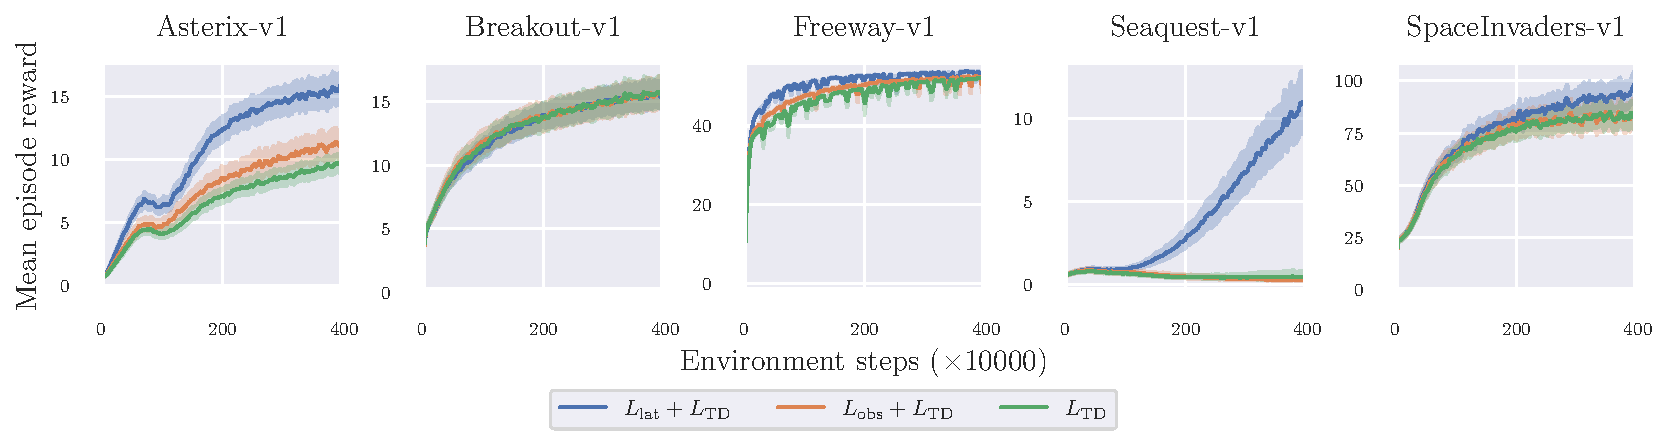
\includegraphics[width=\textwidth]{figures/understanding/rlc2024_minatar.pdf}
    \caption{Auxiliary task setup: Performance of all losses on the observation space as given without changes to the environment.}
    \label{fig:understanding:aux}
\end{figure}

\begin{figure}[t]
    \centering
    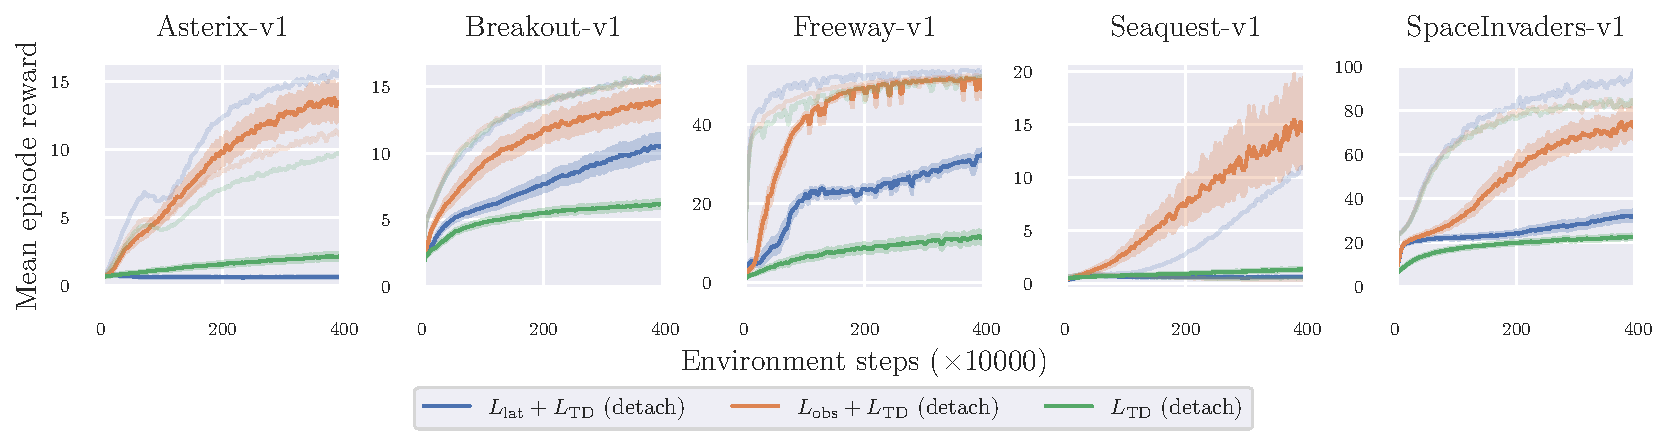
\includegraphics[width=\textwidth]{figures/understanding/rlc2024-detach_minatar.pdf}
    \caption{Stand-alone setup: Performance of all losses on the observation space as given without changes to the environment. The DQN baseline is using random features, which are not updated, to verify that learning features is indeed superior to a random feature baseline.}
    \label{fig:understanding:sta}
\end{figure}

\textbf{Auxiliary task learning vs general purpose feature learning (\autoref{fig:understanding:aux} and \autoref{fig:understanding:sta}):}
First, we compare both the auxiliary task and stand-alone feature learning scenarios.
As expected from prior work \parencite{jaderberg2016reinforcement,schwarzer2021dataefficient,farebrother2023protovalue}, in all cases using an auxiliary loss performs no worse (and often better) than vanilla DQN.
We find that as expected from \autoref{insight:understanding:3}, latent self-prediction is a stronger auxiliary loss function than observation reconstruction in three out of five environments.
However, when using the general-purposes losses alone, we clearly see observation reconstruction performing significantly better than latent self-prediction, which fails to learn any relevant features in several cases. This verifies \autoref{insight:understanding:1}.


Curiously, in the case of the Seaquest environment, we find that using observation prediction alone outperforms using it as an auxiliary task strongly, and performs on par with the auxiliary task variant of the latent self prediction loss.
Seaquest also has the sparsest reward structure in the test suite, which can make it a challenging environment for DQN. In this case, features based purely on the observed transition might allow for better policy learning.

This highlights that no algorithm is clearly superior in all settings and the reward and observation structure is very relevant for the performance of each loss.


\begin{figure}[t]
    \centering
    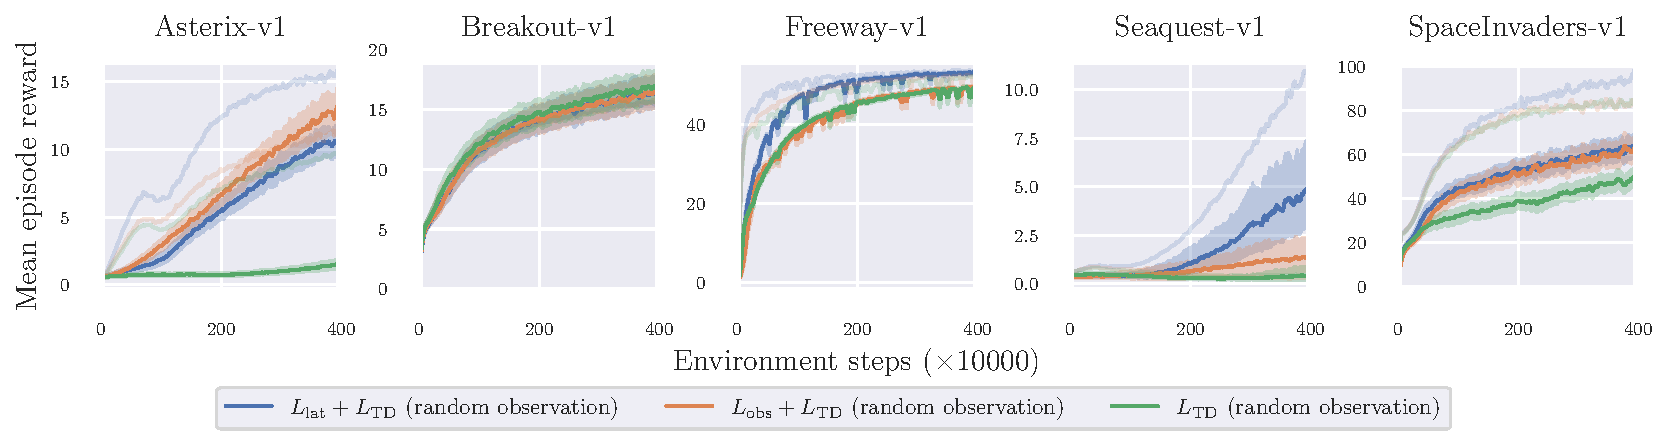
\includegraphics[width=\textwidth]{figures/understanding/rlc2024-distorted-fixed_minatar.pdf}
    \caption{Distorted observation function with a random transformation.}
    \label{fig:understanding:dist}
\end{figure}

\textbf{Observation space distortions (\autoref{fig:understanding:dist}):} To test the impact of changing the observation function, we sample a random binary matrix and multiply it to the flattened observation vector. We then reshape the observation to the original shape again.

All algorithms show themselves to be strongly impacted by this random observation distortions, which suggests that our claim of invariance of self-prediction relies too strongly on the linear gradient-flow limit.
This can in part be explained by the use of a convolutional layer in the standard baseline implementation of DQN which we adapted.
However, we still find that at least on two environments (Seaquest and Freeway), the latent self-prediction auxiliary task is able to recover more of the original performance than either observation prediction or DQN.
The DQN baseline seems to suffer the most from the introduction of the observation change, which suggests that correlations of the existing observation space play an important role in learning correct value function prediction.

Overall, we find that \autoref{insight:understanding:2} does not fully translate to the more complex test setting.
In part, this may be explained by the fact that the original observation spaces of the test environments already violate our assumptions for the one-hot encoding.
In addition, introducing linear correlation might not impact non-linear model learning in the same way it would impact linear models.
This highlights the need for more in-depth research on the interplay between given observation space and feature learning.

\begin{figure}[t]
    \centering
    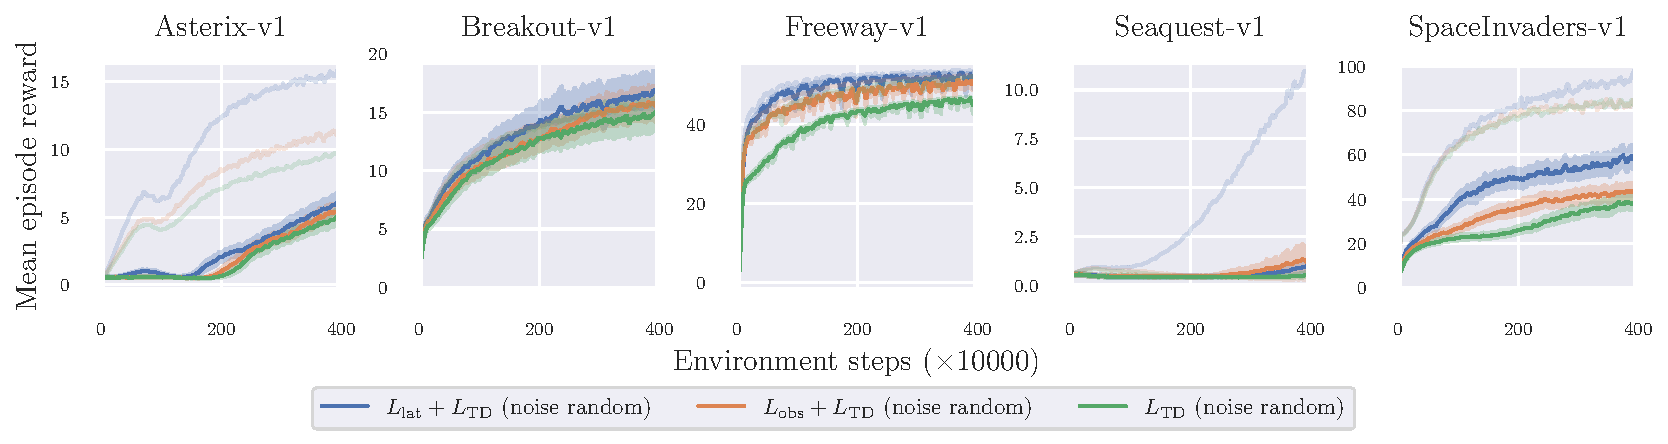
\includegraphics[width=\textwidth]{figures/understanding/rlc2024-noise-random_minatar.pdf}
    \caption{Appending random noise channels.}
    \label{fig:understanding:ran}
\end{figure}

\begin{figure}[t]
    \centering
    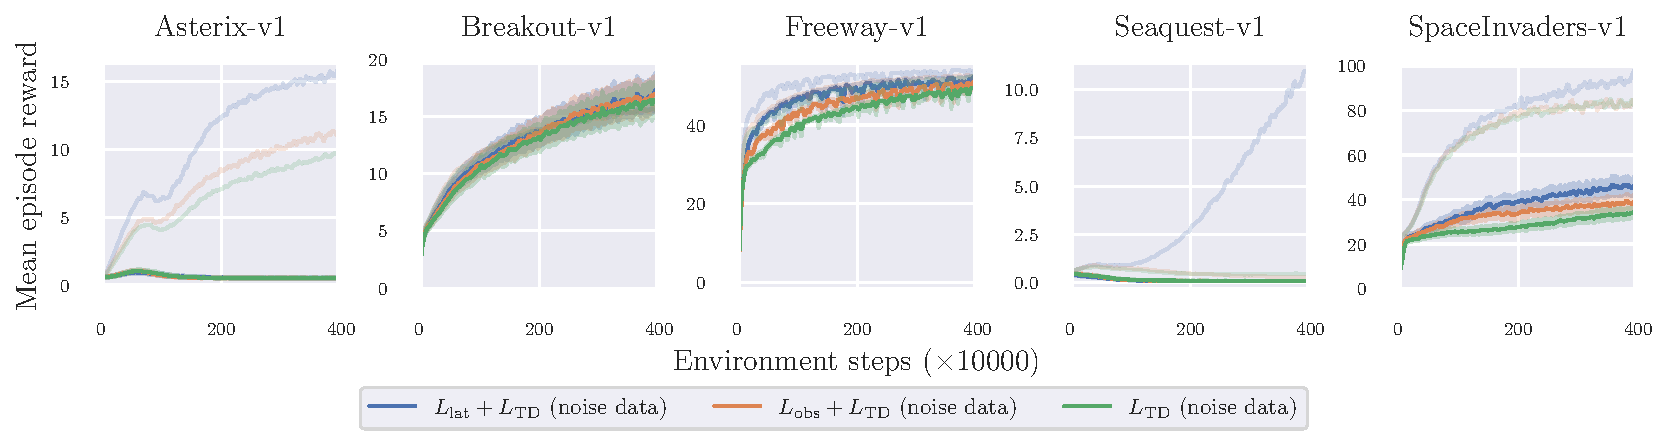
\includegraphics[width=\textwidth]{figures/understanding/rlc2024-noise-data_minatar.pdf}
    \caption{Appending structured noise channels using the Freeway environment.}
    \label{fig:understanding:dat}
\end{figure}

\textbf{Distractions (\autoref{fig:understanding:ran} and \autoref{fig:understanding:dat}):}
As our results are dependent on the spectral structure of the environment, different distraction models can be assumed to have differing impact on the efficacy of the tested losses.
This behavior is dependent on the structure of the noise.
If the distraction does not strongly change the top-$k$ singular or eigenspaces, it will be less problematic for the auxiliary tasks, especially for observation reconstruction.
Testing the impact of different distraction models on the top-$k$ spaces is out of scope for this work, but we conjecture that fully random noise has less structure than distractions following clear patterns.

Therefore, we consider two simple distraction models in our experiments. 
The distractions are concatenated to the original observations along the channel dimension.
First, we use random noise sampled independently for each state from a Bernoulli distribution.
As there is no predictable structure in this noise, we expect all algorithms to be able to deal with this distraction better.
Second, we choose one of the environments at random (Freeway-v1) and concatenate two copies to the observation space of each environment.
The dynamics are obtained by sampling a random action at each timestep independent from the policy and stepping the distraction environment with it.

We find a small advantage in some environments to using the latent self-prediction loss and using random noise, and no clear advantage from any algorithm in the structured noise case.
Structured noise poses a much larger challenge to most algorithms, completely preventing learning in several cases.
This partially validates that not only the presence or absence of noise matters, but also how it changes relevant quantities, e.g. the eigenvalues of the transition kernel.

In the continuous control experiments presented in \autoref{app:understanding:mujoco_results}, we find that the self-prediction loss performs generally better than in the MinAtar suite.
As the observation and reward structure differs between these two benchmark suite, this observation lends more credibility to our claims that the observation structure impacts the performance of algorithms.

\section{Conclusions}

When choosing an RL approach to use, practitioners are overwhelmed with a variety of loss function choices, without clear indication which one will be preferable in what scenario.
In our work, we introduce analytically tractable notions of distractions and observation functions.
With these we predict the performance of latent self-prediction and observation reconstruction as stand-along feature learning methods and auxiliary tasks, and study our theoretical insights empirically.
Our evaluation lends credibility to the use of simple surrogate models to obtain practically relevant insights into algorithmic performance.
However, in several cases we also find deviations between our predictions and more complex benchmarks.
Therefore, while we claim that our theoretical models have the ability to guide the choice of algorithms for applied settings, there is still a sizeable gap between theory and practice that remains to be bridged in future work.

We also note that our experiments showed substantial differences in behavior of auxiliary losses both within and across benchmarks and different noise distractions.
Previous work that studied the effect of distraction \parencite{nikishin2021control,voelcker2022value,ni2024bridging} did not discuss their distraction model in detail. 
In light of our results, we suggest that empirical research should be careful about the choice of benchmark and experimental setup and discuss the implications of the empirical setup explicitly.

On the empirical side the surprising effectiveness of the observation prediction loss on the Seaquest environment highlights the fact that even within benchmark suites, differences in the reward functions and observation models can lead to differing rankings between algorithms.
This further highlights the necessity of studying the structure of MDPs and to design algorithms that are robust to different structures, or adapt to them automatically.

Overall, we can conclude that model-based auxiliary tasks can be very helpful to structure latent representations in a way that complements the task of value function learning.
More importantly for the overall project of this thesis, we now have our first concrete example of an algorithm that leverages both a general-purpose method, predicting latent features, and a decision-aware method, in this case TD learning, and shows that there exists a synergy between these methods for stabilizing feature learning!

However, we have so far only used the model learning to stabilize the feature space.
Instead, we can also use the learned model itself to improve value function learning by generating additional data from the model in a Dyna style algorithm.
In the next chapter we will take a look at such model-based methods.
We will first investigate the idea of decision-aware learning in observation space models.
In the following chapter, we will show that combining latent self-prediction with decision-aware model learning greatly improves the stability of the IterVAML paradigm.
    \chapter{Value-gradient Aware Model Learning}
\label{chap:vagram}

\begin{quote}
    This chapter is based on \longfullcite{voelcker2022value}.
\end{quote}

\section{Introduction}
% \ac{mbrl} is a sample-efficient approach to obtain a policy for a given control problem. 
% It solves the control optimization into two interleaved stages: model learning and policy learning or planning. 
% In the \emph{model learning} stage, an approximate model of the environment is learned which is then utilized in the \emph{planning} stage to generate new experience without having to query the original environment. 
% Often this process is repeated by continually updating the model with new experience and replanning based on the updated model. 
While our previous chapters have focussed on representation learning, we will now shift our focus to decision-aware model learning.
Model-based RL is an enticing paradigm for scenarios in which samples of the true environment are difficult or expensive to obtain, such as computationally intensive simulators, real-world robots, or environments involving humans, since the model can be used to generalize the policy to unseen regions of the state space. 
The approach has received a lot of attention and significant progress has been made in the field \parencite{dyna,deisenroth2011pilco,levine2013guided,hafner2020dream,moerland,schrittwieser2020mastering}.

One of the core problems of model-based policy learning methods, however, is that the accuracy of the model directly influences the quality of the learned policy or plan \parencite{schneider1997exploiting,kearns2002near,ross2012agnostic,talvitie2017self,luo2018algorithmic,janner2019mbpo}. 
Model errors tend to accumulate over time, and therefore long-term planning under approximate models can lead to suboptimal policies compared to the performance achievable with model-free approaches.
This is especially prevalent in settings with complex dynamics, such as robotic environments with discontinuities, which can be hard to model with common function approximation methods.
These model approximation errors are nearly impossible to avoid with current methods due to limits of function approximation in model and value learning algorithms, which cannot fully capture the full distribution over dynamics functions perfectly, and the use of finite datasets.

Hence, it is important that a model is accurate \textit{where it counts} for the planning procedure, by modelling dimensions and data points that have a higher impact on the planning.
But this objective is not captured in most current \ac{mbrl} methods, which generally use \ac{mle}-based losses to train a parametric model of the environment without involving information from the planning process.
In \autoref{chap:background} we reviewed this problem under the term \emph{objective mismatch}~\parencite{lambert202objective}, but the problems has been investigated in several earlier works as well \parencite{joseph2013reinforcement}.
Several recent papers have investigated the objective mismatch~\parencite{abachi2020policy,zhang2021learning,ayoub2020model,grimm2020value,grimm2021proper,nikishin2021control}, but currently theoretical investigation and understanding of possible approaches do not perform well when applied to complex deep learning based approaches~\parencite{lovatto2020decision} or the proposed approaches rely on heuristics which might not be applicable generally~\parencite{nair2020goal}.

\noindent \textbf{Summary of Contributions}. In this chapter, we present the \textit{Value-Gradient Weighted Model Learning}~(VaGraM) which rescales the mean squared error loss function with gradient information from the current value function estimate.
We first discuss the disadvantages of the Value-Aware Model Learning framework \parencite{vaml, itervaml} by conducting an empirical analysis of the optimization behavior, and form two hypotheses for the lack of empirical performance gain despite theoretical intuition: (a) the theory does not account for the complicated learning behavior of value functions discussed in the preceding two chapters and (b) it also does not address how to counter problems that arise when the state space is yet insufficiently explored in early stages of the model training.
Our experiments show, qualitatively and quantitatively, that the VaGraM loss impacts the resulting state and value prediction accuracy, and that it solves the optimization problems of previously published approaches.
Beyond pedagogical domains, we show that VaGraM performs on par with a current state-of-the art \ac{mbrl} algorithms in more complex continuous control domains, while improving robustness to irrelevant dimensions in the state-space and smaller model sizes.

The VaGraM algorithm again follows our overarching idea of combining a general-purpose objective, mean-square error minimization, and a decision-aware one, reweighing by value function sensitivity.
Instead of using shared network layers, here we demonstrate that we can also modify loss functions to directly incorporate both idea.

\section{Value-Gradient Weighted Model Learning}
\label{sec:vagram:method}

One of the main drawbacks of model-based reinforcement learning is the fact that model errors propagate and compound when the model is used for planning \parencite{schneider1997exploiting,kearns2002near,talvitie2017self}.
As discussed in \autoref{chap:background:objective}, one attempt at addressing the objective mismatch is the IterVAML loss \parencite{itervaml}
\begin{align}
    &\mathcal{L}_V(\hat{p}, p, \mu) = \int \mu(\state,a) \bigg|\underbrace{\int p(\state'|\state,a)V(\state')\mathrm{d}\state'}_{\text{environment value estimate}}  - \underbrace{\int \hat{p}(\state'|\state,a) V(\state') \mathrm{d}\state'}_{\text{model value estimate}}\bigg|^2 \mathrm{d} (\state,a).
\end{align}

\textcite{itervaml} presents error bounds for both model and value learning steps of the iteration, but did not test the algorithm to ascertain whether the presented error bounds are sufficient to guarantee {a strong algorithm in practice}. 
As our analysis in the previous two chapters shows, fitting value functions accurately enough to meet the assumptions of \textcite{itervaml} is difficult when dealing with neural networks and partially covered state-action spaces.
As we discuss now, IterVAML provides an intuitive fix to the model-mismatch problem, yet faces two key issues which lead to empirical ineffectiveness \textcite{lovatto2020decision}. 
These phenomena are investigated and verified in detail in \autoref{sec:vagram:experiments}.

\paragraph{Value function evaluation outside of the empirical state-action distribution} IterVAML suffers when randomly initialized models predict next states that are far away from the current data distribution or if the optimization procedure leads the model's prediction outside of the covered state space. 
Since the value function has only been trained on the current data distribution, it will not have meaningful values at points outside of its training set.
Nonetheless, these points can still achieve small value prediction errors if, due to the optimization process, the value function outside the training distribution happens to have the same value at the model prediction as the environment sample.
We therefore require that our value-aware loss function should not directly depend on the value function at the model prediction, since these might be potentially meaningless.

\paragraph{Suboptimal local minima} %
The predictions of the model can converge to a solution that is far away from the environment sample in the state space if the prediction's and the ground truth's values are equal.
In this case, we find that the model-based value prediction often performs poorly after updating the value function as two different states are not guaranteed to have the same values after updating.
We expect that the updated model loss forces the model prediction to a new solution, but due to the non-convex nature of the VAML loss in the state space, the model can get stuck or even diverge.
This is especially prevalent when the previous minimum is situated outside of the empirically covered state space.
A stable value-aware loss function should therefore have only one minimum in the state space that lies within the empirical state distribution. 
The full loss function will likely still admit additional local minima in the parameter space due to the non-linear nature of the model itself, but the global optimum should coincide with the true model and the loss function should be convex in the state space.

Note that several of these issues are related to the fact that previous empirical works using the IterVAML loss have used observation-space models.
As we discussed in the previous chapters, stabilizing value learning by regularizing the learned latent-space features alleviates many issues around divergence and uninformative values.
In this chapter, we will also constrain ourselves to observation-space models, to understand the issues facing value-aware learning in detail.
In \autoref{chap:cvaml} we will show how combining IterVAML style losses with latent self-prediction can lead to strong value aware learning.

\subsection{Approximating IterVAML with the value function gradient}
From our insights, we obtain two criteria: a stable loss should not depend on the value function at states not captured in the dataset, and it should not admit local minima beyond an \ac{mle} solution.
To derive a loss function that fulfils these requirements, we start from the assumption that the difference between the model prediction and the environment next states $\state'$ are small.
This is implicitly required by many \ac{mbrl} approaches, since an MLE model cannot be used to estimate the next state's value otherwise. 
{We also assume that the model has small transition noise, akin to the model assumptions underlying MSE regression, otherwise the difference between a model sample and the next state sample might be large.}
Under this assumption, the IterVAML loss can be approximated by a Taylor expansion of the value function, where we denote the expansion of $V$ around a reference point $\state'$ as $\hat{V}_{\state'}$ and obtain $\hat{V}_{\state'}(\state) \approx V(\state') + (\nabla_\state V(\state)|_{\state'})^\intercal (\state - \state')$.
Using this expansion at the next state sample $\state'_i \in \mathcal{D}$ collected from the environment for each tuple independently instead of the original value function, the VAML error can be stated
\begin{align}
    \hat{\mathcal{L}}_{\hat{V}}=&\frac{1}{|\mathcal{D}|}\sum_{\{\state_i,a_i,\state'_i\}\in\mathcal{D}}{\left(V(\state'_i) - \int \hP_\theta(\state'|\state_i,a_i) (V(\state'_i) + (\nabla_\state V(\state)|_{\state'_i})^\intercal (\state' - \state'_i)) \mathrm{d}\state'\right)^2}\\
    =&\frac{1}{|\mathcal{D}|}\sum_{\{\state_i,a_i,\state'_i\}\in\mathcal{D}} {\left(\int \hP_\theta(\state'|\state_i,a_i) \left((\nabla_\state V(\state)|_{\state'_i})^\intercal(\state' - \state'_i) \right) \mathrm{d}\state'\right)^2}.
\end{align}

This objective function crucially does not depend on the value function {at unknown state samples, all $\state'_i$ are in the dataset the value function is trained on}, which solves the first of our major problems with the VAML paradigm.

We can simplify the objective above even further if we restrict ourselves to deterministic models of the form $\hat{\state}'_i = f_\theta(\state,a)$.
Since VAML requires the expectation of the value function under the model and the environment to be equal, we can exchange the probabilistic model with a deterministic one as long as we assume that the mean value function under the true environment is close to the empirical estimate of the value function from a single sample.
We explore the prerequisites and consequences of this assumption further in \autoref{chap:cvaml}.
The model loss is now
\begin{align}
    \sum_i {\left((\nabla_\state V(\state)|_{\state'_i})^\intercal (f_\theta(\state_i,a_i) - \state'_i) \right)^2} \label{eq:vagram:taylor_vaml}.
\end{align}

We can see that the objective is similar to a mean squared error regression with a vector that defines the local geometry of the objective function. This vector can be interpreted as a measure of sensitivity of the value function at each data point and dimension. In regions where the value function changes significantly, the regression pushes the model to be very accurate. 

\subsection{Bound between Value-Aware Model Learning and VaGraM}
\label{app:taylor_bound}

The error in Taylor approximation $\mathcal{R}(V, x', f_\theta(s,a))$ is bounded by $\frac{M}(x'){2}\|x' - f_\theta(x,a)\|^2$ with M dependent on the Hessian of the value function. 
Plugging this into the VAML loss and assuming worst case approximation errors, we obtain an upper bound on the VAML error

\begin{align}
    &\E_{x',x,a \sim D}\left[\left(V\left(f_\theta(x,a) \right) - V(x_0')\right)^2\right] \\
    = &\E_{x',x,a \sim D}\left[\left((\nabla_s V(x)|_{x'})^\intercal (f_\theta(x,a) - x') + \mathcal{R}(V, x',f_\theta(x,a))\right)^2\right]\\
    \leq &\E_{x',x,a \sim D}\left[\left(\left|(\nabla_x V(x)|_{x'})^\intercal (f_\theta(x,a) - x')\right| + \left|\mathcal{R}(V, x_0', f_\theta(x,a))\right|\right)^2\right]\\
    \leq &\E_{x',x,a \sim D}\left[{\left(\left|(\nabla_x V(x)|_{x'})^\intercal (f_\theta(x,a) - x')\right| + \frac{M(x')}{2}\|x' - f_\theta(x,a)\|^2\right)^2}\right]\\
    \leq &2\cdot\E_{x',x,a \sim D}\left[{\left((\nabla_x V(x)|_{x'})^\intercal (f_\theta(x,a) - x')\right)^2}\right] + 2\cdot\E_{x',x,a \sim D}\left[\frac{M(x')^2}{4}\|x' - f_\theta(x,a)\|^4\right].
\end{align}

The parameter $M(x')$ depends on the Hessian at each state $x'$.
However, computing the Hessina of the value function is an expensive operation, and therefore we found it infeasible to compute this term in practice.
Alternatively, we could attempt to find a hyperparameter $M \geq M(x')$ for all $x'$ and bound the loss this way.
However, we can only tune this parameter approximately and did not achieve strong performance as we are forced to chose very conservative bounds.
In this case, we are effectively only optimizing the polynomial term which is akin to performing mean squared regression (except for using the fourth power instead of the second).

\subsection{Preventing spurious local minima}
\begin{figure}[!t]
\centering
    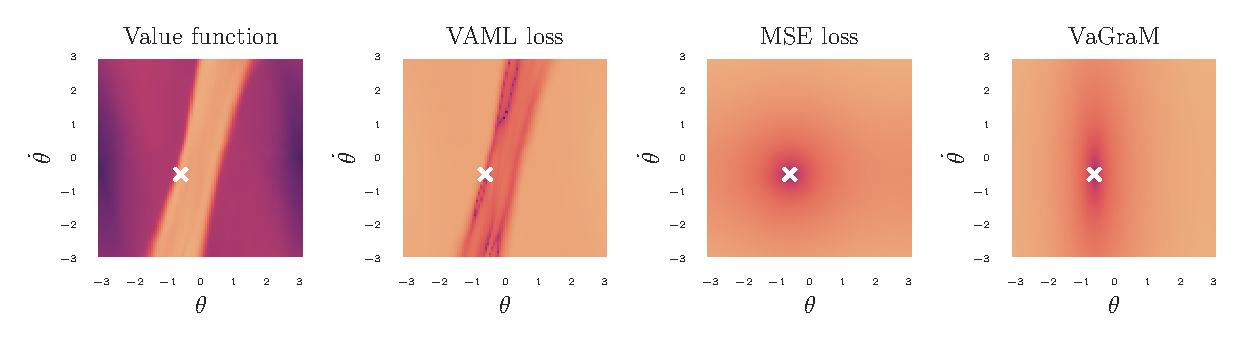
\includegraphics[clip, trim=0.cm 0.5cm 0.cm 0.45cm, width=\textwidth]{figures/vagram/all_losses.pdf}
    \caption{{Visualization of discussed loss function with regards to a reference point marked with the white cross and the corresponding value function on the Pendulum environment. For the value function, darker color indicates a lower value. In the loss figures, darker color indicates how large the loss is if the model predicts $(\theta, \dot{\theta})$ instead of the reference sample marked in white. The VAML loss has a complex non-linear shape in the state space that follows iso-lines of the value function, while MSE and VaGraM are centered around the sample. For VaGraM, the rescaling of the MSE in the direction of high gradient along the $\theta$ axis is visible. Due to \autoref{eq:vagram:upper_bound}, the scaling is aligned with the axis of the coordinate system and not rotated to fit the value function closer.}}
    \label{fig:vagram:all_losses}
\end{figure}


The formulation above retains one problem: \autoref{eq:vagram:taylor_vaml} does not constrain the solution for each $(\state,a,\state')$ tuple sufficiently.
For each $(\state,a,\state')$ tuple, the loss function only requires that the difference between the model and environment sample be orthogonal to the gradient of the value function, which describes a hyperplane of solutions.
These predictions can lie arbitrarily far away from the environment sample, which breaks the assumption underlying the Taylor approximation that the model prediction is within a small region of the expanded state point.
This can be made more clear by looking at the loss for a single datapoint.
Writing $\text{dim}(\states)$ for the dimensionality of the state space, we obtain
\begin{align}
    &\min_\theta \left((\nabla_\state V(\state)|_{\state'})^\intercal f_\theta(\state,a) \right) ^2\\
    =&\min_\theta \left(\sum_{n=0}^{\text{dim}(\states)} (\nabla_\state V(\state)|_{\state'})_n \cdot f_\theta(\state,a)_n\right)^2.
\end{align}

Assuming that $f$ is flexible and can predict any next state $\state'$, the optimal solution is obtained from an under-determined linear system of equations
\begin{align}
    \sum_{n=0}^{\text{dim}(\states)} (\nabla_\state V(s)|_{\state'})_n \cdot f_\theta(x,a)_n = 0
\end{align}

This system admits far more solutions than either the corresponding IterVAML loss or a mean squared error, and many of them will achieve arbitrary large value prediction errors.
In fact, the equation describes a hyperplane of minimal solutions consisting of every weight vector that is orthogonal to the gradient of the value function at the reference sample, with $\text{dim}(\states) - 1$ free variables.
Therefore we need to enforce the closeness of the model prediction and the environment sample, since the Taylor approximation is only approximately valid in a close ball around the reference sample.

Again, one way to achieve this closeness is by adding the second order Taylor term, which results in an additional MSE loss term.
However, as discussed, finding a good $M$ is expensive in practice.
Therefore, we approach the solution to this problem as outlined below.

\subsection{Bounding the first-order Taylor loss}

To prevent these suboptimal solutions and achieve our second design goal, we consider an upper bound on the value-gradient loss by applying a corollary of the Cauchy-Schwarz inequality $\left(\sum_{i=1}^n x_i \right) ^2 \leq n \sum x_i^2$ to change the square of the sum with a sum of squares.
We denote the diagonal matrix with vector $a$ on the diagonal as $\text{diag}(a)$  and rephrase the sum as a vector-matrix multiplication
\begin{align}
    &\sum_{\{x_i,a_i,x'_i\}\in\mathcal{D}} {\left((\nabla_x V(x)|_{x'_i})^\intercal(f_\theta(x_i,a_i) - x'_i) \right)^2}\\
    \leq {\text{dim}(\states)} &\sum_{\{x_i,a_i,x'_i\}\in\mathcal{D}}\left((f_\theta(x_i,a_i) - x'_i)^\intercal\text{diag}(\nabla_x V(x)|_{x=x'_i})^2(f_\theta(x_i,a_i) - x'_i) \right) \label{eq:vagram:upper_bound}.
\end{align}

This reformulation is equivalent to a mean squared error loss function with a per-sample-dimension diagonal scaling matrix.
Because the scaling matrix is positive semi-definite by design, each summand in the loss is a quadratic function with a single solution as long as the derivative of the value function does not become zero in any component.
Therefore this upper bound assures our second requirement: the loss function does not admit spurious local minima.\footnote{We note that state dimensions are ignored for points in which components of the value function become zero, potentially leading to spurious minima as before solutions, but in practice this rarely happens for more than a few points.}

To give an intuitive insight into all the discussed loss functions, we visualized each one for a pedagogical environment, the Pendulum stabilization task.
The resulting loss curves can be seen in \autoref{fig:vagram:all_losses}.
The VAML loss has a complicated shape that depends on the exact values of the value function while both MSE and our proposal have a paraboloid shape.
Compared to MSE, our proposed loss function is rescaled to account for the larger gradient of the value function in the $\theta$ axis.

\section{Experiment: Analyzing model learning}
\label{sec:vagram:experiments}

\begin{figure}[t]
\begin{center}
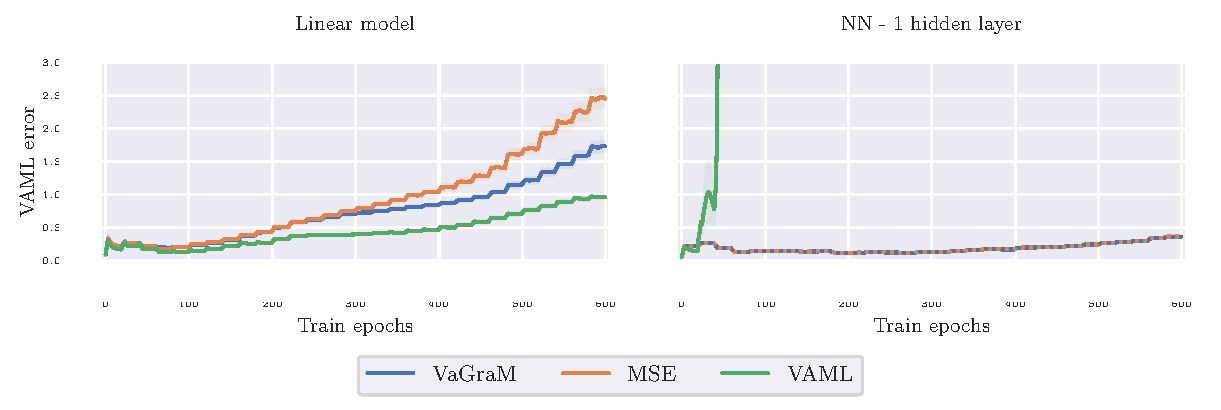
\includegraphics[width=\linewidth]{figures/vagram/pendulum_joint.pdf}
\end{center}
\caption{\textbf{Evolution of the VAML loss over changing value functions on the Pendulum domain}. Lines denote the mean and shaded areas show standard error over 8 model initialization and data set samples per model. In the linear setting, VAML achieves the lowest VAML error, while VaGraM is able to significantly outperform MSE. In the NN setting, VAML diverges rapidly, {while VaGraM and MSE converge to approximately the same solution.}}
\label{fig:vagram:iterated_pendulum_training}
\end{figure}

We compare the performance of VaGraM, with both MSE and VAML on a pedagogical environment with a small state space and smooth dynamics to gain qualitative insight into the loss surfaces. 
We use the Pendulum environment, a canonical control problem in which an under-actuated pendulum must be swung and stabilized to an upright position.
We use the implementation provided by \textcite{brockman2016openai}.
To learn the policy and its value function, we use the SAC algorithm \parencite{sac}.
The original IterVAML analysis assumed that the value function was obtained using approximate value iteration (AVI) \parencite{gordon1995stable,ernst2005tree,farahmand2010error}. We use SAC instead of a full AVI for stability in large scale experiments and discuss a proper extension of the VAML loss to SAC in \autoref{app:vagram:vaml_sac}. We find that the difference in loss is negligible and therefore use SAC together with VAML throughout our experiments.
More information on the implementation and hyperparameters of all of our experiments can be found in \autoref{app:vagram:implementation}. 

To simplify the setup of the evaluation, we decided to investigate the model losses without model-based value function learning.
This allows us to focus solely on the loss functions, without taking into account the inter-dependency between model and value function updates.
Instead of the model-based loop, we used the SAC algorithm in a model-free setup to estimate the value function.
We saved the intermediate value functions after each epoch of training, corresponding to 200 environment steps, and optimized the models using stochastic gradient descent on the respective loss function, updating the value function used for the loss every 1000 model training steps.
As the MLE loss, we used the mean squared error which assumes a Gaussian model with fixed variance.

To compare the optimization, we used two architectures, a linear model without feature transformations and a neural network with a single hidden layer and 16 neurons.
We obtained a dataset of states sampled uniformly over the whole state space and used the environment transition function to compute ground truth next state samples.
Finally, we evaluated each models VAML error with regards to the current value function on a held out dataset and plotted the results in \autoref{fig:vagram:iterated_pendulum_training}.

\paragraph{Dependency on value function estimates.}
The first cause for lacking empirical performance with VAML that we discussed in \autoref{sec:vagram:method} was that the algorithm can predict successor states with incorrect value function as they lie outside of the data distribution.

In our experiment we find that a linear regression model remains stable under all three loss functions, VaGraM, MSE and VAML.
But when using a flexible function approximation, the VAML loss converges in the first iteration with the given value function, but then rapidly diverges once the value function is updated.
When investigating the mean squared error of the VAML solution, we find that the model finds a stable minimum of the VAML loss outside of the reachable state space of the pendulum.
This confirms our hypothesis that flexible VAML models can find solutions outside of the empirical state space distribution, which are unstable once we update the value function.
VaGraM remains stable even with flexible function approximation and achieves a lower VAML error than the MSE baseline when using a model with insufficient capacity to represent the dynamics.

\paragraph{Single solution convergence.}
In the experiment, we see that the MSE and VaGraM models converge to a similar solution when using a neural network. 
This leads us to the conclusion that our loss function really only admits a single solution and that this solution coincides with the mean square error prediction when the function approximation has sufficient capacity to model the dynamics function with high precision.
On the other hand, the VAML network converges to solutions that are far away from the environment sample measured in the $L_2$ norm and it cannot recover from these spurious minima due to the complex optimization landscape.


\section{{Experiment: Model-based Continuous Control}}

\begin{figure}[t]
\begin{center}
    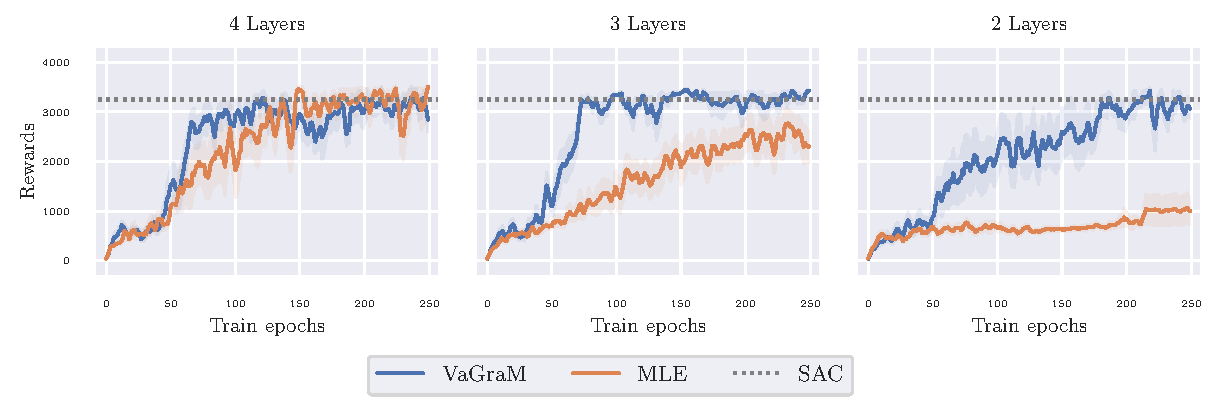
\includegraphics[clip, trim=0.2cm 0.0cm 0.4cm 0.0cm, width=1.\linewidth]{figures/vagram/fig_2.pdf}
\end{center}
    \caption{\textbf{Performance of VaGraM and MLE models with reduced model size}. The dotted lines correspond to the final performance reported for model-free SAC (grey, approx. 3200). Shaded area represents standard error over 16 repeated runs. VaGraM continues to solve the task almost unimpeded, while MLE is unable to even stabilize the Hopper when using a two layer neural network.}
    \label{fig:vagram:pendulum_small}
\end{figure}
Due to the limited complexity of the pendulum environment, the quantitative differences between the mean squared error and VaGraM are at times insignificant in this setting.
The dynamics function of the environment can be approximated sufficiently well with a simple neural network and one hidden layer.

The underlying theory supporting VAML states that a value-aware loss is preferable to a mean squared error loss in a setting where the capacity of the model is too small to fully approximate the problem or the state space contains dimensions that are irrelevant for the control problem.
To test whether our loss function is superior to a maximum likelihood approach in these cases, we used the Hopper environment from the OpenAI gym benchmark \parencite{brockman2016openai}. 
As a deep learning based Dyna algorithm, we chose \ac{mbpo} \parencite{janner2019mbpo} and ran all of our experiments using the implementation provided by \textcite{pineda2021mbrl}.
We kept the structure of the \ac{mbpo} algorithm and models and replaced the model loss function with VaGraM.

\subsection{Hopper with reduced model capacity}
In the first experiment, we decreased the network size of the used neural network ensemble.
\textcite{janner2019mbpo} use fully connected neural networks with four hidden layers and 200 neurons per layer.
To test the performance of the algorithm under smaller models, we ran tests with two and three layer networks and 64 neurons per hidden layer.
The results are shown in \autoref{fig:vagram:pendulum_small}.
As before, when using a sufficiently powerful function approximation, we see no difference between the maximum likelihood approach and VaGraM, suggesting that the networks are flexible enough to capture the true environment's dynamics sufficiently close for planning.
But when reducing the model size, the maximum likelihood models quickly lose performance, completely failing to even stabilize the Hopper for a short period in the smallest setting, while VaGraM retains almost its original performance.

\subsection{Hopper with distracting dimensions}


\begin{figure}[t]
    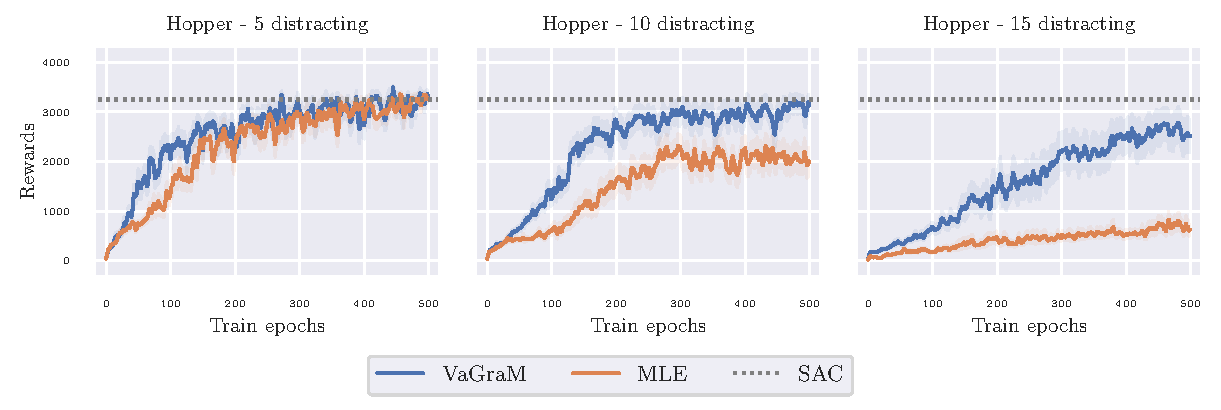
\includegraphics[clip, trim=0.2cm 0.0cm 0.4cm 0.0cm, width=1.\linewidth]{figures/vagram/fig_1.pdf}
    \caption{\textbf{Performance of VaGraM and MLE models with distracting state dimensions}. The dotted lines correspond to the final performance achieved by both algorithms on the Hopper task without distraction (grey, approx. 3200). Shaded area represents standard error over 16 repeated runs. VaGraM achieves significantly higher returns than the MLE baseline, especially in the most challenging setting with 15 distracting dimensions.}
    \label{fig:vagram:pendulum_distraction}
\end{figure}

To show that VaGraM is able to achieve good performance in a setting where there are additional dynamics in the environment that do not contribute to the control problem, we appended distracting dimensions to the Hopper observations.
This mirrors the experimental setup used in \autoref{chap:understanding}.
These are independent of the original environment state space and reward function, and evolve under non-linear and discontinuous dynamics (details in \autoref{app:vagram:implementation}).
A setting with distracting dimensions is known to pose difficulty for model-based control algorithms \parencite{stone2021thedc} and neural networks struggle to model non-linear, discontinuous dynamics, so with an increasing number of dimensions the task becomes harder.

The results of this experiment are shown in \autoref{fig:vagram:pendulum_distraction}.
When using five distracting dimensions, both models are able to capture the dynamics sufficiently well to achieve comparable reward to the original environment.
When increasing the number of dimensions, the performance of the MLE model deteriorates, as more and more of its capacity is used to model the added dynamics.
VaGraM continues to be able to achieve reward even under the presence of distracting dimensions, since the gradient of the value function with regards to the state dimensions which are irrelevant to the control problem becomes small over training.
Still, the performance of VaGraM also suffers with increasing dimensions: when adding 20 distracting dimensions, neither algorithm is able to stabilize the Hopper consistently.
In this case, the value function approximation cannot differentiate sufficiently between the relevant and irrelevant dimensions with the amount of environment samples provided.

In summary, we find that VaGraM is able to deal with challenging distractions and reduced model capacity significantly better than a MLE baseline. This validates that our algorithm is really value-aware and can use the value function information {to improve the performance of a model-based controller in settings where the model is unable to fully represent the environment.}

\section{Related work}

Several authors have noted on the problem of learning models that align with the goal of obtaining a good policy. The proposed approaches fall into three broad categories: value-function or policy dependency, representation learning, and data resampling.

Inspired by VAML, \textcite{abachi2020policy} present a method that seeks to align the policy gradients under a learned model with the gradients under the true environment. Similar to our proposal, \textcite{doro2020gradient} also proposed to reweigh samples in a log likelihood loss, but used policy search as the reinforcement learning approach and did not account for individual state dimensions. \textcite{nikishin2021control} show an approach to directly optimizing the policy performance on the real environment by learning a model with implicit differentiation. \textcite{asadi2018equivalence} show that the original VAML loss coincides with a Wasserstein distance in the model space under the assumption that the value function is Lipschitz smooth. We find that all of these approaches suffer from similar scaling issues as VAML and have not been shown to lead to strong empirical performance outside of toy settings.

\textcite{grimm2020value} characterize the space of possible solutions to the model learning problem under different restrictions given by value functions and policies, and propose to learn models that are value-equivalent, similar to \textcite{vaml}. In a follow-up work \textcite{grimm2021proper} expand on this idea and show that their principle can be used to improve the MuZero algorithm \parencite{schrittwieser2020mastering}. However, these works do not discuss the optimization challenges in actually finding such value-equivalent models, they mostly characterize the space under different value functions and policies, and present an orthogonal research direction to this chapter.


An alternative to characterizing the problem in the state space of the MDP are representation learning approaches, which seek to map the original states to a latent representation that is more amenable to control. Such approaches include Value Prediction Networks \parencite{oh2017value}, Embed-to-Control \parencite{10.5555/2969442.2969546} and related proposals \parencite{levine2020prediction,cui2021controlaware}. \textcite{zhang2021learning,kemertas2021towards,kemertas2022approximate} build on the idea of bisimulation metrics \parencite{ferns2004metrics,ferns2011bisimulation} which seeks to characterize the difference between MDPs by finding a state mapping that is reward-invariant under policy and value function. 
In the following chapters, we show how to extend IterVAML and related approaches to include state-representation learning.

\textcite{lambert202objective} hypothesize that the objective mismatch could be solved by reweighing the training buffer for model learning to prioritize data points with high value. These are more likely to matter for obtaining an optimal policy. A similar proposal was evaluated empirically by \textcite{nair2020goal}. Contrary to our work however, this technique cannot account for the differing impact of the state space dimensions and scaling, since the data points are weighted as a whole.


\section{Conclusion}
This chapter presents a core issue with using decision-aware methods such as VAML and IterVAML.
It shows that prior work does not account for two important optimization phenomena that appear when learning models with empirical value function approximations.
To mitigate this issue, we introduced an attempt at getting the best of both decision-aware and general purpose learning, Value-Gradient Weighted Model Learning (VaGraM).
VaGraM is a novel loss function to train models that model a dynamics function \emph{where it matters} for the control problem.
We highlighted how VaGraM counters the issues of pure decision-aware learning and show the increased stability of the training procedure when using our loss in a pedagogical environment.

On the Mujoco benchmark, VaGraM performs on par with maximum likelihood estimation when using large neural network models.
However, introducing additional complications to the problem results in drastic performance impacts for MLE based models, which highlights the necessity for value function aware losses in challenging environments and settings in which sufficient model capacity cannot be guaranteed.
In these cases, value-awareness can greatly increase the performance of Dyna algorithms by focusing the model learning procedure on relevant aspects of the state space.
% In future work we seek to scale our loss function to image-based RL, where relevant state space dimensions can vary over a task due to shifting camera angles. 
% Furthermore, we seek to derive a related value-aware approach for partially observable domains that can take the state inference problem into account.

While VaGraM is an important step towards our goal of unifying general purpose and decision-aware learning, it does not take into account the importance of feature learning.
As we saw in the previous chapter, latent self-prediction objectives can lead to features which are aligned with the goal of value prediction.
In the next chapter we will see that these losses can also serve as auxiliary losses to stabilize the problems with IterVAML that we observe in this chapter.
    \chapter{Calibrated Latent Models for Value Aware Model Learning}
\label{chap:cvaml}

\todo[inline]{Merge papers properly}

\begin{quote}
    This chapter is based on \longfullcite{voelcker2025calibrated} and \longfullcite{voelcker2023lambda}.
\end{quote}

\newcommand{\rev}[1]{#1}

\section{Introduction}
In model-based reinforcement learning, an agent collects information in an environment and uses it to learn a model of the world. 
This model is used to improve value estimation and policy learning~\parencite{dyna,deisenroth2011pilco, Hafner2020Dream,schrittwieser2020mastering}.
However, as environment complexity increases, learning a model becomes more and more challenging. 
This leads to model errors which propagate to value function learning~\parencite{schneider1997exploiting,kearns2002near,talvitie2017self,lambert202objective}.
In such cases, deciding what aspects of the environment to model is crucial.

The paradigm of \emph{value-aware model learning} (VAML)~\parencite{vaml} and \emph{value-equivalence}~\parencite{grimm2020value,grimm2021proper} addresses this by training models that lead to accurate value estimation.
Prominent value-aware model learning approaches are MuZero~\parencite{schrittwieser2020mastering} and IterVAML~\parencite{itervaml}.
The MuZero loss has been shown to perform well in discrete~\parencite{schrittwieser2020mastering,ye2021mastering} and continuous control tasks~\parencite{hansen2022temporal,hansen2024tdmpc}, but has received little theoretical investigation.
On the other hand, IterVAML is a theoretically motivated algorithm but not commonly used in empirical work.
We show that MuZero and IterVAML can be unified in a family of losses, which we term $(m,b)$-Value-Aware Model Losses ($(m,b)$-VAML).
The name stresses the two core hyperparameters: the model rollout steps, $m$, and steps used to estimate the bootstrapped value function target, $b$.

The $(m,b)$-VAML losses are used as surrogate losses in place of other value- or model learning losses.
Therefore, it is important to ask whether they are calibrated \parencite{steinwart2008support}.
A calibrated loss does not lead to suboptimal minima when the function class includes optimal functions for the original target loss.
% We focus our investigation on stochastic environment models, which parameterize a distribution over the next state prediction.

\textbf{Research question:} This chapter has three parts, each with a theoretical and empirical section. We answer two questions about the $(m,b)$-VAML family: (a) What variants of the $(m,b)$-VAML losses are well-calibrated to recover correct models and value functions? (b) Do we observe problems with uncalibrated losses when using standard architectures, especially deterministic latent-space models?

\textbf{Contributions:} 
As our main theoretical contribution, we mathematically analyze the family of $(m,b)$-VAML algorithms.
We prove that all members of this loss family are uncalibrated when used with a stochastic environment model.
To counter this issue, we derive a novel loss variant.

In the second part, we address issues arising from the way current algorithms in the $(m,b)$-VAML family are commonly implemented.
We prove that a stochastic model class is not necessary to learn a single-step decision-equivalent model in stochastic environments.
This validates the practice of primarily using deterministic models in empirical work~\parencite{oh2017value,schrittwieser2020mastering,hansen2022temporal}.
Empirically we find that using stochastic models can still lead to improved performance, although this is environment-dependent.
% We,  corroborate our results empirically in challenging continuous control tasks \parencite{tunyasuvunakool2020dmcontrol} and show that correcting the $(mb,b)$-VAML leads to empirical performance gains.


\section{Background}

\textbf{Reinforcement Learning:} We consider a standard as presented in \autoref{chap:background:mdp}.
As a brief reminder, we review the notation.
The policy-conditioned transition kernel is $\P^\pi(x'|x) = \int \P(x'|x,a) \pi(a|x) \mathrm{d} a.$
The value is the unique stationary point of the Bellman operator $$[\mathcal{T}_{\P^\pi} V](x) = \EEX{\pi}{r(x_0,a_0) + \gamma  \EEX{\P^\pi}{V(x_1)}|x_0=x}.$$
This operator can be extended to a multi-step version as $$[{\mathcal{T}}^b_{\P^\pi} V](x) = \EEX{\pi,\P}{\sum_{n=0}^{b-1} \gamma^n r(x_n,a_n) + \gamma^b {V(x_b)}\Big|x_0=x}.$$
We also define $[\mathcal{T}_{\P^\pi}^0 V](x) = V(x).$

\textbf{Model-based RL:} In this chapter, we focus on value learning with model data, which is commonly referred to as Dyna~\parencite{dyna}.
We use $\hat{p}$ to refer to a stochastic model, and $\hat{f}$ for deterministic models.
When a model is used to predict the observation $x'$ from $x,a$ (such as the model used in MBPO \parencite{mbpo}) we call it an \emph{observation-space models}.
Alternatively, \emph{latent-space models} of the form $\hat{p}(z'|z, a)$ are used, where $z\in\mathcal{Z}$ is a representation of a state $x\in\mathcal{X}$ given by $\varphi: \mathcal{X} \rightarrow \mathcal{Z}$.
Observation-space models predict next states in the representation of the environment, while latent-space models reconstruct learned features of these states.

The notation $x^{(n)}$ refers to the $n$-th step in a rollout starting in state $x$ in the environment.
We will use $\hat{x}^{(n)}$ to refer to samples from the $n$-th step model prediction and write $\EEX{\hat{p}}{\cdot}$ as a shorthand for $\EEX{{x}^{(m)}\sim \hat{p}(\cdot|x)}{\cdot}$.

\section{The Value-Aware Model Learning framework}
\label{sec:model_losses}

\begin{figure*}[t]
    \centering
    \begin{minipage}{0.68\linewidth}
        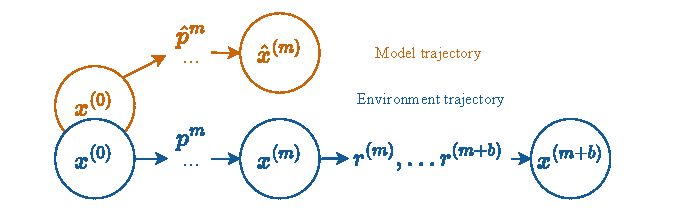
\includegraphics[width=\textwidth]{figures/lambda/mb_loss.drawio.pdf}
    \end{minipage}
    \begin{minipage}{0.31\linewidth}
    \begin{align*}
        &\hat{\mathcal{L}}^{\P^\pi}_{m,b}\left(\hat{p},\hat{V}|x\right)\\
        = &\biggl|{\color{newgreendeal}\underbrace{\hat{V}\roundb{\hat{x}}}_\mathrm{model}} - 
        \biggl[ {\color{newbluedeal} \underbrace{[\mathcal{T}_{\P^\pi}^b \hat{V}]\roundb{x^{(m)}} }_\mathrm{environment} } \biggr]_\mathrm{sg}\biggr|^2
    \end{align*}
    \end{minipage}
    \caption{Sketch of $(m,b)$-VAML. The loss is computed from an {\color{newgreendeal}$m$-step model} and a {\color{newbluedeal} $(m+b)$-step environment trajectory}. It is the difference between the estimated value of the {\color{newgreendeal}$m$-th model state}, and the $b$-step Bellman operator starting from the {\color{newbluedeal} $m$-th environment state}.}
    \label{fig:loss_graphic}
\end{figure*}

The losses of the decision-aware learning framework share the goal of finding models that provide good value function estimates.
Instead of simply learning a model using maximum likelihood estimation, the losses are based on differences in value prediction.

\subsection{Iterative Value Aware Model Learning}

While IterVAML has been discussed in \autoref{chap:background:objective} and \autoref{chap:vagram}, we will now focus on its relationship to other loss functions.
To achieve this, we reintroduce the IterVAML loss with a small modification, an $m$-step and $k$-sample variant.
The loss function introduced previously can be seen as a single-step and single-sample variant of this more general loss.

This more general IterVAML still computes the difference between the expected value under the model and samples in the environment
\begin{equation}\label{eq:itervaml}
\begin{aligned}
     &{\mathcal{L}}^{\P^\pi}_{\mathrm{IterVAML}, m}\left(\hat{p},V|x, x^{(m)}\right) \\
    & \quad = \biggl|\mathbb{E}_{\hat{p}^m} \squareb{V\roundb{\hat{x}^{(m)}}} - 
    \squareb{\EEX{\P^\pi}{V\roundb{x^{(m)}}}}_\mathrm{sg}\biggr|^2 \\
    & \quad \approx \biggl|\frac{1}{K}\sum_{k=1}^K \squareb{V\roundb{\hat{x}_k^{(m)}}} - 
    \squareb{V\roundb{x^{(m)}}}_\mathrm{sg}\biggr|^2. 
\end{aligned}
\end{equation}
%
We will use $\mathcal{L}_{\mathrm{IterVAML}, m}$ to refer to the expectation-based version, and $\hat{\mathcal{L}}^k_{\mathrm{IterVAML}, m}$ to refer to the sampling-based version.
To reduce notational complexity, we drop the action dependence in all following propositions; all results hold without loss of generality for the action-conditioned case as well.
The expectation-based version of the IterVAML loss has an important relationship to the error of computing the model's Bellman operator compared to the true environments Bellman operator.

\begin{restatable}{proposition}{IterVAMLEqual}{\textcite{itervaml}}\label{prop:1_1}
    Let $\P^\pi$ be the policy-conditioned transition kernel of an MDP and let $V: \mathcal{X} \rightarrow \mathbb{R}$ be a function.
    Let $\hat{p}(\cdot|x)$ be a model so that ${\mathcal{L}}^{\P^\pi}_{\mathrm{IterVAML}, 1}\left(\hat{p},V|x\right) = 0$.
    Then $\squareb{\mathcal{T}_{\P^\pi} V }(x) = \squareb{\mathcal{T}_{\hat{p}} V }(x)$.
\end{restatable}

Intuitively, a model achieving $0$ loss can be used instead of the ground truth environment when computing the Bellman operator.
The set of models that achieve $0$ IterVAML error is equal to the set of proper value-equivalent models for the value estimate $\hat{V}$ \cite{grimm2021proper}.

\subsection{The $(m,b)$-VAML Family}
The MuZero loss~\parencite{schrittwieser2020mastering} was introduced to unify the value function and model learning components of an MBRL algorithm.
It can be interpreted as a variation of the IterVAML loss that uses a single sample estimate of the Bellman Operator and a bootstrapped target estimate. 
To unify the losses, we present them in a single equation with two important hyperparameters: $m$, the number of steps in the trajectory that the loss is computed over, and $b$, the number of steps for the multi-step Bellman operator.
We refer to this unified family of losses as $(m,b)$-Value Aware Model Losses (VAML)
\begin{align}
    & \hat{\mathcal{L}}^{\P^\pi}_{m,b}\left(\hat{p},\hat{V}|V_\mathrm{tar},x, x^{(m)}\right) = \biggl|\hat{V}\roundb{\hat{x}^{(m)}} - 
    \squareb{[\mathcal{T}_{\P^\pi}^b V_\mathrm{tar}]\roundb{x^{(m)}}}_\mathrm{sg}\biggr|^2, \label{eq:dal_loss}
\end{align}
%
where $V_\mathrm{tar}$ is a target network \parencite{mnih2013playing}.
We denote the stop-gradient operation with $\squareb{\cdot}_\mathrm{sg}$.
Note that samples from the real environment are used to approximate $[\mathcal{T}_{\P^\pi}^j \hat{V}]$.
% Furthermore, the loss requires a re-parametrizeable function class if used with stochastic models.
The loss function and the relation of the model and environments rollout are visualized in \autoref{fig:loss_graphic}.

Several works use variations of this loss:
The original MuZero algorithm \parencite{schrittwieser2020mastering} and follow-up work \parencite{ye2021mastering,antonoglou2022planning} use $m\geq1$ and $b\geq1$.
In continuous control, $m\geq1,b=1$ has been used in the TD-MPC line of work \parencite{hansen2022temporal,hansen2024tdmpc}.
% The IterVAML loss \parencite{itervaml} can be recovered by choosing $i\geq1, j=0$, 
When using only a single sample $k=1$, the sample-based IterVAML loss is equal to $\hat{\mathcal{L}}^{\P^\pi}_{m,0}$.
Finally, regular model-free TD learning corresponds to $m=0,b\geq1$.


\section{Analysis of decision-aware losses in stochastic environments}
\label{sec:theory_1}
The goal of learning in MBRL is to recover an (approximately) optimal model and to learn a correct value function.
As we have shown, minimizing the IterVAML loss perfectly results in a model that leads to a correct Bellman Operator.
However, in practice, the inner expectation of the IterVAML loss has to be replaced by a sampling-based approximation.
In addition, $(m,b)$-VAML is often used to update the value function directly in addition to the model.
We show when this leads to learning correct models and value functions asymptotically.
An overview of our conclusions can be found in \autoref{tab:bias_overview}.
Proofs are found in \autoref{app:main_proofs}.
\subsection{Calibration of surrogate loss functions}

Formally, we ask whether the surrogate $(m,b)$-VAML is \emph{calibrated}.
%A calibrated surrogate loss has a set of minimizers that is a subset of the set of minimizers of some target loss.
Intuitively, a calibrated surrogate loss does not select a suboptimal function for the target loss.
\begin{definition}[$\mathcal{F}$-Uncalibrated surrogate losses]
    Let $\mathcal{L}_\mathrm{tar}(f,x,x^{(m)})$ be a loss function defined over samples from an MDP.
    Let $\hat{\mathcal{L}}_\mathrm{sur}$ be a surrogate function for the loss.
    Let $\mathcal{F}^*$ be a set of minima of $\mathcal{L}_\mathrm{tar}$ with $\mathcal{L}_\mathrm{tar}(f^*,x,x^{(m)}) = 0$ for all $f^* \in \mathcal{F}^*.$
    Let $\mathcal{F}$ be a function class with $\mathcal{F}^* \subseteq \mathcal{F}$.
    A surrogate function is $F$-\emph{uncalibrated} for the target loss if there exists an MDP and a state $x$ so that 
    $$\argmin_{f \in \mathcal{F}} \mathbb{E}_{x^{(m)}\sim\P^\pi(\cdot|x)}\left[\mathcal{L}_\mathrm{sur}(f,x,x^{(m)})\right] \not\subseteq \mathcal{F}^*.$$
\end{definition}
%
A prominent example of an $\mathcal{F}$-uncalibrated loss is Bellman Residual Minimization (BRM), which results in the \emph{double sampling issue}.
We reviewed this issue and a proof in \autoref{chap:background:rl} and will see how related issues arise here.
Recall that while in BRM the target loss is minimized by the ground-truth value function, BRM actually chooses a function that minimizes an additional variance term.

We will show that some issues introduced by naively using $(m,b)$-VAML can be fixed with a tractable modification to the loss.
We call such cases \emph{resolvable}.


\begin{table*}
{\footnotesize
\centering
    \begin{tabular}{l l|c|c|c}
        && IterVAML &  MuZero &  Model-free TD \\
        \multicolumn{2}{l|}{$(m\geq1,b=0)$} &  $(m\geq1,b\geq1)$& $(m=0,b\geq1)$\\\hline
        Det. model,& det. env & {\color{newbluedeal} calibrated} & {\color{newbluedeal} calibrated} & {\color{newbluedeal} calibrated} \\
        Stoch. model,& det. env & {\color{newgreendeal} uncalibrated (resolvable)} & {\color{uoftred} uncalibrated (for VF updates)} & {\color{newbluedeal} calibrated}\\
        Det. model,& stoch. env & {\color{newbluedeal} calibrated} & {\color{newbluedeal} calibrated}  & {\color{newbluedeal} calibrated} \\
        Stoch. model,& stoch. env & {\color{newgreendeal} uncalibrated (resolvable)} & {\color{uoftred} uncalibrated (for VF updates)} & {\color{newbluedeal} calibrated} \\\hline
        \multicolumn{2}{l|}{Can update model} & {\color{newbluedeal} $\checkmark$} & {\color{newbluedeal} $\checkmark$}& \color{uoftred} X \\
        \multicolumn{2}{l|}{Can update VF}   & \color{uoftred} X & {\color{newgreendeal} $\checkmark$ (for det. model)}  & {\color{newbluedeal} $\checkmark$}
    \end{tabular}}
    \caption{Comparison of the major design choices in the $(m,b)$-VAML framework. IterVAML and MuZero can be used to update the model, while MuZero and Model-free TD learning can be used to update the value function. All model-based losses are uncalibrated when applied to stochastic model classes. In addition, MuZero suffers a bias when used for value function prediction which cannot be surmounted with an easy modification to the loss function.}
    \label{tab:bias_overview}
\end{table*}

\subsection{Model learning bias with stochastic models}

Most prior work uses $(m,b)$-VAML with deterministic models.
Exceptions are \textcite{voelcker2022value} and \textcite{antonoglou2022planning}, but neither changes the loss functions to account for the model parametrization.
For a stochastic model class, $(m,0)$-VAML is uncalibrated for the target loss $\mathcal{L}_\mathrm{IterVAML}$.

We begin with analyzing the loss for $m\geq1$ and $b=0$.
For simplicity we assume that $V_\mathrm{tar} = \hat{V}$.
%
\begin{restatable}{proposition}{IterVAMLUncal}\label{prop:2_1}
    Let $\hat{\mathcal{L}}^{\P^\pi}_{m\geq1,0}(\hat{p},V|x,x^{(m)})$ be the surrogate loss for $\mathcal{L}_{\mathrm{IterVAML}, m}^{\P^\pi}(\hat{p}, V|x, x^{(m)})$.
    Let $\P^*$ be the set of all distributions $p$ for which $\EEX{p}{V(\hat{x}^{(m)})} = \EEX{\P^\pi}{V(x^{(m)})}.$
    There exist an MDP and a class of distributions $\mathbb{P}$ with $\P^\pi \in \P^* \subseteq \mathbb{P}$ so that $$\Argmin_{\hat{p} \in \mathbb{P}} \mathbb{E}_{\hat{p}}\left[\hat{\mathcal{L}}^{\P^\pi}_{m\geq1,0}(\hat{p},V|x,x^{(m)})\right] \not\subseteq \P^*.$$
    Therefore $\hat{\mathcal{L}}_\mathrm{model}$ is $\P$-\emph{uncalibrated}.
\end{restatable}
%
When using samples from a stochastic model to compute the loss function in \autoref{eq:dal_loss}, we are left with a variance error term that is closely related to the double-sampling problem
\begin{align}
 &\mathbb{E}_{\hat{p}}[\hat{\mathcal{L}}^{\P^\pi}_{1,0}(\hat{p},V|x)] = {\mathcal{L}}^{\P^\pi}_{\mathrm{IterVAML}, 1}\left(\hat{p},V|x,x'\right) + \mathrm{Var}_{\hat{p}}\left(V(\hat{x})\right).
\end{align}
%
In the classic double-sampling problem, we cannot correct the variance term as we do not have oracle access to the environment.
Here the issue is our model, and we can generate multiple samples from it.
Therefore, we can estimate this variance term from samples and correct the loss.
This correction is reminiscent of \textcite{antos2008learning} but is simpler to obtain as we only need model samples.

To obtain the correction, we define $\hat{\mu}_{\hat{p}}^{m,k} = \frac{1}{k}\sum V(\hat{x}_k^{(m)})$, the empirical estimator of the expected return in \autoref{eq:itervaml}.
The variance of this estimator can be estimated as $\widehat{\mathrm{Var}}_{\hat{p}}^{m,k} = \frac{1}{k} \sum (V(\hat{x}_k^{(m)}) - \mu_{\hat{p}}^{m,k})^2$.
With this, we can define a new loss which can be computed with at least two samples from the model.
We refer to the loss as \emph{Corrected VAML} (CVAML).

\begin{restatable}{proposition}{IterVAMLVar}\label{prop:2_2}
    Let $\hat{\mathcal{L}}_{\mathrm{CVAML}, m}^{k} = \hat{\mathcal{L}}^k_{\mathrm{IterVAML}, m} - \widehat{\mathrm{Var}}_{\hat{p}}^{i,k}.$
    $\hat{\mathcal{L}}_{\mathrm{CVAML}, m}^{k}(\hat{P}, V|x, x^{(m)})$ is a calibrated surrogate loss for $\mathcal{L}_{\mathrm{IterVAML}, m}^{\P^\pi}(\hat{P}, V|x, x^{(m)})$.
\end{restatable}

Analogous to the IterVAML case, the sample-based $(m,b \geq 1)$-VAML loss is an uncalibrated loss for learning a model.
To address this issue, we can introduce a corresponding variance correction term.

\subsection{Value learning bias in stochastic environments}
\label{sec:muzero_bias}

We now show this issue also affects the value function learning with the MuZero loss.
The problem lies in the use of the bootstrapped Bellman target together with a multi-step value rollout.
In an MDP, the values of two states $x$ and $y$ are not guaranteed to be equal (or even particularly close) just because they share an ancestor state, unless we make assumptions about the variance of the value function over successor states.
However, the MuZero loss still minimizes the difference in value functions between these two states.

We show that the MuZero loss therefore is not guaranteed to recover the correct value function, even when we have a perfect (stochastic) model.
To formalize the issue, we compare the solution found with $(m,b)$-VAML with the regular TD loss function
\begin{align}
    &\mathcal{L}_\mathrm{TD}(V|V_\mathrm{tar}, x^{(m)},x^{(m+1)},r^{(m)}) \nonumber\\
    &\quad=\left(V(x^{(m)}) - \left[r^{(m)} + \gamma V_\mathrm{tar}(x^{(m+1)})\right]\right)^2.
\end{align}

\begin{restatable}{proposition}{MuZeroValue}\label{prop:2_3}
    Let $\mathcal{L}_\mathrm{TD}(V|V_\mathrm{tar}, x^{(m)},x^{(m+1)},r^{(m)})$ be the target loss, and let $\hat{\mathcal{L}}^{\P^\pi}_{m,1}\left(\P^\pi,V| V_\mathrm{tar},x, x^{(m)}\right)$ be the surrogate loss. 
    Let $\mathcal{V}$ be a set of functions so that $[\mathcal{T}_{\mathcal{P}^\pi}V_\mathrm{tar}] \in \mathcal{V}$ for some target function $V$.
    Then, for any $V_\mathrm{tar}$ that is not a constant function, $$ \Argmin_{\hat{V} \in \mathcal{V}} \mathbb{E}_{\P^\pi}\squareb{\hat{\mathcal{L}}^{\P^\pi}_{m,1}(\P^\pi, \hat{V}| V_\mathrm{tar}, x, x^{(m)})} \not \subseteq [\mathcal{T}_{\P^\pi} V_\mathrm{tar}].$$
    Therefore, $\hat{\mathcal{L}}^{\P^\pi}_{m,1}$ is $\mathcal{V}$-uncalibrated.
\end{restatable}


\begin{figure*}[t]
    \centering
    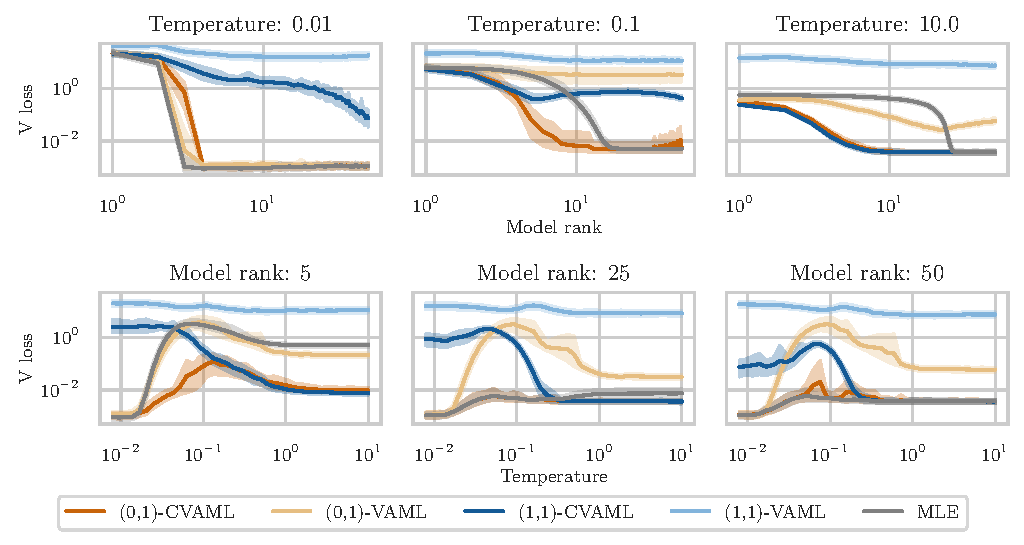
\includegraphics[width=.9\linewidth]{figures/lambda/plts/v_loss_comparison.pdf}
    \caption{Results for the garnet experiments. 
    In the top row, we show the mean squared error of the value function prediction using different latent sizes $k$, over three different temperatures. 
    In the bottom row, we vary the temperature and show results for three values of $k$. 
    Shaded regions are bootstrapped confidence intervals of the mean at 95\% over 1000 independent problems. 
    With the exception of deterministic problems (left), the CVAML loss reliably results in the lowest value prediction error. }
    \label{fig:garnet}
\end{figure*}

The problem in the loss function again depends on the variance of the value function with regard to the model.
%
To overcome this issue, we can introduce another variance correction term, similar to $\hat{\mathcal{L}}_\mathrm{CVAML}$. 
This retains the advantage that the MuZero loss is used for both model and value updates.
However, as we average over the value prediction from the model, we only guarantee that 
\begin{align}
\mathbb{E}_{\hat{p}}\left[V(\hat{x}^{(m)})\right] \approx \mathbb{E}_{\P^\pi}\Bigl[[\mathcal{T}_{\P^\pi}^b V_\mathrm{tar}](x^{m})\Bigr],
\end{align}
not that the values for each state are correct.
These are necessary for accurate planning or policy improvement, therefore, it is still important to use a loss variant with $m=0$ for learning accurate values for each state.

\subsection{Discussion of theoretical results}
While the problem resulting from the use of stochastic models is resolvable, the MuZero loss is still insufficient for learning \emph{per state} value function with stochastic models.
In addition, we observe issues with learning accurate value functions with the $(m\geq1,b\geq1)$-VAML loss even after correctly calibrating it.
% However, the major issue is the use of the MuZero loss ($j\leq1$) for updating the value function estimate.
If the corrected loss is used to update the model, and a standard model-free or model-based value estimate is used as the value function learning target, the correct value function can be learned.
% Such an algorithm can also interleave model-free and model-based updates, such as the procedure used in \textcite{voelcker2024mad}.

\begin{boxinsight}[Calibrated losses]
    To obtain a calibrated loss, we propose using $\hat{\mathcal{L}}_\mathrm{CVAML}$ to update the model and $\hat{\mathcal{L}}^{\hat{p}}_{0,j}$, or $\hat{\mathcal{L}}^{\P^\pi}_{0,j}$, to update the value function.
\end{boxinsight}

\section{Calibration impact on finite state MDPs}
\label{sec:empirical1}

To test our findings, we run the $(m,b)$-VAML losses on small, finite state Garnet problems \parencite{bhatnagar2007incremental}.
Every problem is generated by sampling $m$ successor states for each state $x_i$, and parameterizing the transitions with random weights $\omega_{i,j}$ for all successor states $x_j$.
The transition distribution is given by $p(x'_i|x_j) = {e^{\omega_{i,j}/\tau}}/{\sum_j e^{\omega_{i,j}/\tau}}$.
Varying the temperature $\tau$ we can interpolate between a deterministic transition and a $m$ uniform one.

The models are parameterized with two learnable matrices $\varphi \in \mathbb{R}^{n\times k}$ and $\psi \in \mathbb{R}^{n\times k}$ so that $\hat{p}_k(x_i| x_j)  = \mathrm{softmax}(\hat{\omega}_{i,j}) = \mathrm{softmax}(\varphi_i^\top \psi_j)$.
By varying $k$ we create a low-rank constraint.
As \textcite{vaml} shows, $(m,b)$-VAML should be used when the model has insufficient capacity to represent the environment.
As a baseline, we use the model $\hat{p}_{\mathrm{KL}, k}\in \argmin_{\hat{p}} \mathrm{KL}(p||\hat{p})$.

We focus solely on value estimation in the Garnet MDPs with a fixed policy to simplify the experimental setup.
We also use the ground truth reward function.

\textbf{Results:}
The numerical results are graphed in \autoref{fig:garnet}.
For the deterministic ground truth environment, we see no benefit from using a calibrated $(m,b)$-VAML.
We find that the algorithms are able to exploit the non-linear softmax function to achieve very accurate models in deterministic environments.
However, even small amounts of stochasticity prevent this solution.

As the stochasticity increases, we see an advantage for the calibrated losses.
$(1,1)$-VAML is not able to achieve any good results even when the underlying environment is deterministic.
This corroborates the theoretical finding that the error depends on the model's stochasticity and not on the environment.
As we initialize the models with high entropy, $(1,1)$-VAML is unable to learn a high variance value.

Calibrated $(1,1)$-VAML still struggles in environments with low stochasticity.
We find that due to the variance term over value functions, the model is prone to get stuck in local minima as it reduces the value function difference per state faster than the model predictive variance.
% This suggests that the variance correction might be insufficient to achieve good learning in the non-asymptotic regime.
This suggests that a $(m\geq1,0)$-CVAML loss is preferable with stochastic environments.

\section{Latent environment models and auxiliary losses}
All previous results hold independent of the model architecture.
However, in practice, most implementations of decision-aware models use deterministic latent model structures \cite{schrittwieser2020mastering,ye2021mastering,hansen2022temporal,antonoglou2022planning}.

In general, deterministic function approximations cannot capture the full transition distribution in stochastic environments.
However, it is an open question whether a deterministic \emph{latent} model can be sufficient for learning a value-equivalent model, as conjectured by \textcite{oh2017value}.

\subsection{Deterministic models for stochastic environments}

Showing the existence of a deterministic value-aware model relies on the continuity of the transition kernel and involved functions $\varphi$ and $V$.
These are standard assumptions that are necessary to prove the convergence of many algorithms \parencite{bertsekasshreve1978}.

\begin{restatable}{proposition}{DeterministicModel}\label{prop:3_1}
    Let $\mathcal{X}$ be a compact, connected, metrizable space. Let $p$ be a continuous kernel from $\mathcal{X}$ to probability measures over $\mathcal{X}$. Let $\mathcal{Z}$ be a metrizable space. Consider a bijective latent mapping $\varphi: \mathcal{X} \rightarrow \mathcal{Z}$ and any $V: \mathcal{Z} \rightarrow \mathbb{R}$. Assume that they are both continuous. Denote $V_\mathcal{X} = V \circ \varphi$.
    
    Then there exists a measurable function $f^*: \mathcal{Z} \rightarrow \mathcal{Z}$ such that we have $V(f^*(\varphi(x))) = \EEX{p}{V_\mathcal{X}(x^{(1)})}$ for all $x \in \mathcal{X}$.

    Furthermore, the same $f^*$ is a minimizer of the expected IterVAML loss:
    $$f^* \in \argmin_{\hat{f}} \EEX{\P^\pi}{\hat{\mathcal{L}}_{\mathrm{IterVAML},1}(\hat{f},V_\mathcal{X}|V_\mathcal{X},x,x^{(1)})}.$$
\end{restatable}

We can conclude that given a sufficiently flexible function class $\mathcal{F}$, $(m,b)$-VAML can recover an optimal deterministic model for value function prediction.
Note that our conditions solely ensure the \emph{existence} of a measurable function; the learning problem might still be very challenging.


\subsection{Auxiliary losses for latent-space models}

While the original MuZero algorithm only uses the MuZero loss to update the latent embedding, dynamics model, and value function estimation, several more recent works add auxiliary stabilizing losses \parencite{ye2021mastering,hafner2021mastering,hansen2024tdmpc,voelcker2024mad}.
These allow the model to learn meaningful transitions even before the value function is properly approximated, which helps e.g. in sparse-reward environments.

Most prior works use some form of Bootstrap-your-own-latent (BYOL) \parencite{grill2020bootstrap} loss, which minimizes the difference between the next states encoding $\varphi(x^{(m)})$ and the model prediction $f^m(x^{(0)})$.
In the case of linear features, models, and value functions, recent works, discussed in \autoref{chap:understanding}, have shown that such a loss can greatly aid in learning meaningful features for value function prediction \parencite{lyle2021understanding,tang2022understanding,ni2024bridging,voelcker2024when}.

When the difference is computed with an $L_2$, the model loss is
\begin{align}
    & \hat{\mathcal{L}}^{\P^\pi}_{\mathrm{model}, m}\left(\hat{f},
\varphi, \hat{V}|x\right) \nonumber\\
    & ~ = \underbrace{\hat{\mathcal{L}}^{\P^\pi}_{m,b}\left(\hat{f},\varphi, \hat{V}|x\right)}_{m,b\mathrm{-VAML}} + \underbrace{\biggl| \hat{f}^m(\varphi(x)) - \bigl[\varphi(x^{(m)}) \bigr] \biggr|^2}_\mathrm{auxiliary}.
\end{align}

\subsection{Experiments with latent model architectures}

\todo[inline]{Repeat old experiments}

\section{Stochasticity and auxiliary models}
\label{sec:theory_2}

%
The introduction of a stabilizing loss poses a challenge for the result in \autoref{prop:3_1}.
For example, a pre-trained LLM backbone might be used, which is naturally stochastic due to the sampling strategies used to query it.
Therefore, it is still important to have a calibrated surrogate loss for stochastic models, as many use cases make stochastic models attractive.

For a flexible enough model and embedding function class, the perfect BYOL-based model $f^*_\mathrm{aux}$ would predict $\EEX{\P^\pi}{\varphi(x')| x}$.
However, $f^*_\mathrm{aux}$ only coincides with the optimal model under the VAML loss iff
\begin{align}
    \EEX{\P^\pi}{\hat{V}(\varphi(x^{(1)}))} = \hat{V}\biggl(\EEX{\P^\pi}{\varphi(x^{(1)})}\biggr).
\end{align}
This is the case if and only if the value function is linear in the embedding features $\varphi$, which is also referred to as a linear expectation model \cite{wan2019planning}.
However,  learning an embedding in which the value function is linear can be difficult and may not lead to stable model predictions in complex, high-dimensional environments.

\begin{figure*}[t]
\centering
   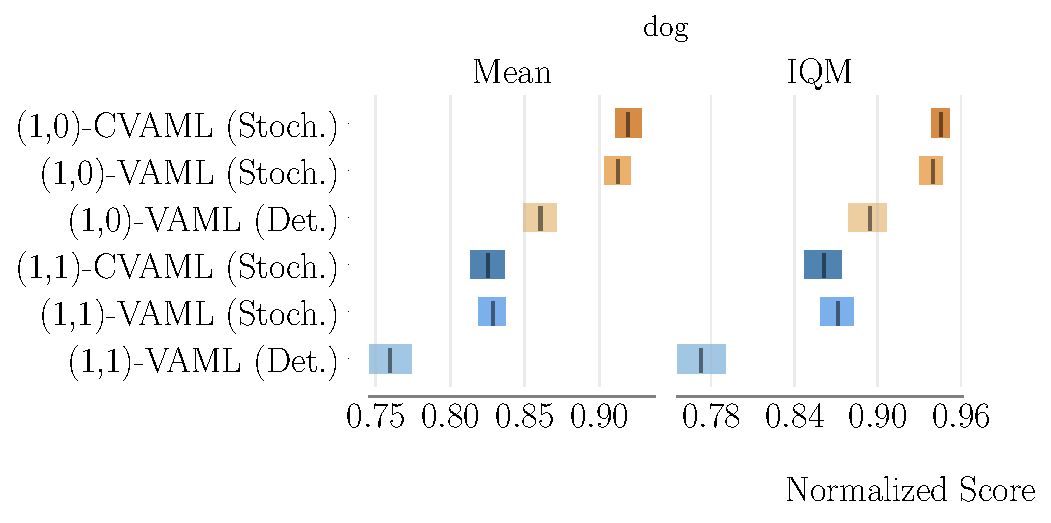
\includegraphics[width=0.5\textwidth]{figures/lambda/plts/agg_dog.pdf} 
   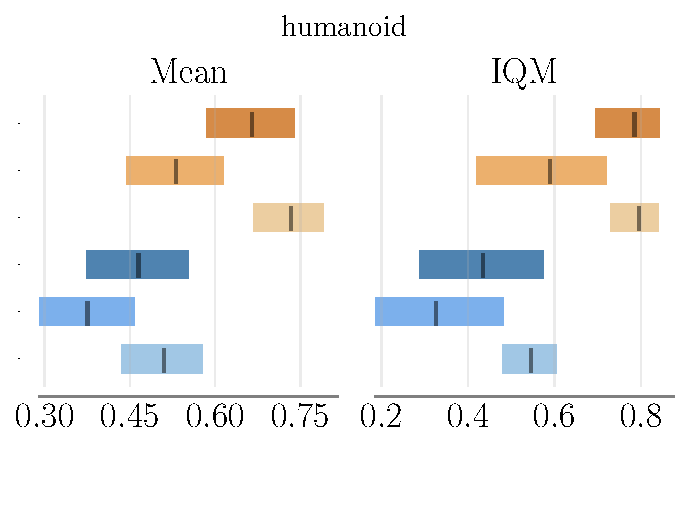
\includegraphics[width=0.33\textwidth]{figures/lambda/plts/agg_hum.pdf} 
   \caption{Results for the latent-space model experiments. We show the aggregate metrics of the final performance on dog (left) and humanoid (right) environments, following \cite{agarwal2021deep}. Calibrating $(1,1)$-VAML leads to a clear improvement in performance in the dog environment, while for $(1,0)$-(C)VAML the difference is less noticeable. This is consistent with our theoretical findings as learning a smaller variance model can be sufficient, but wrong value functions will be learned with a stochastic model when $b\geq1$.}
   \label{fig:agg_results}
\end{figure*}

An exception to the use of deterministic models is the architecture proposed by \textcite{antonoglou2022planning}.
However, their model and auxiliary loss rely on a biased straight-through gradient estimation.
This introduces complications for finding the optima of the loss function and model class.

\section{Calibration experiments with latent-space models}
\label{sec:empirical2}


We examine the impact of the calibrated losses on a subset of DMC environments \cite{tunyasuvunakool2020dmcontrol} encompassing various tasks within the \textit{humanoid} and \textit{dog} domains.
These two domains are the most challenging in the DMC suite, and the standard comparison for current methods \cite{voelcker2024mad,nauman2024bigger}.

We present a comparison between $(m,b)$-CVAML and $(m,b)$-VAML families of losses using stochastic latent models.
The forward models are multivariate Gaussian distributions in the latent space parameterized by MLPs \cite{pets,mbpo,paster2021blast}. 
 
Model rollouts are produced by sequentially sampling latent states from the model conditional on the initial state and an action sequence using the reparametrization trick. 
\begin{align}
&\hat{p}(\hat{z}'|z,a)=\hat{\mu}(z,a) + \hat{\sigma}(z,a)\cdot\varepsilon,\; \varepsilon \sim \mathcal{N}(0,I)
\end{align}

The auxiliary loss for stochastic models is computed as a negative log-likelihood of the next states' latent representations under the current dynamics model.
\begin{align}
    &\mathcal{L}_{\mathrm{aux},m}\left(\hat{p},\varphi\Big|x,a^{(0:m-1)},x^{(m)}\right) \nonumber\\
    &\quad =-\log \hat{p}^m\left(\varphi(x^{(m)})\Big|\varphi(x),a^{(0:m-1)}\right),
\end{align}
where $a^{(0:m-1)}$ is a sequence of actions of length $m$ starting from state $x^{(0)}$.

The actor and the critic are trained with the TD3 algorithm \cite{fujimoto2018addressing}, while the executed policy is obtained from the actor and environment model using MPC \cite{hansen2022temporal}: initialized at the action produced by the actor for the current state this algorithm iteratively refines the action to maximize the expected return.

For $(m,b)$-CVAML, the calibration term is computed by sampling multiple trajectories from the model and calculating the means and variances of next-state values produced by the critic across the different samples.
Additional implementation details are provided in \autoref{app:model_design}.

\textbf{Results:} We show results across both domains in \autoref{fig:agg_results}.
We plot aggregated final performance over 20 random seeds per environment-loss pair with 95\% CI,  estimated with stratified percentile bootstrap \cite{agarwal2021deep}.
\autoref{fig:dmc_reward} shows aggregated learning curves with bootstrapping.

The difference in performance is most noticeable between the $(1,1)$-VAML and -CVAML, as the uncalibrated loss impacts both model and value function learning in this case. 
This effect is less prominent but still present with $(1,0)$-CVAML, where only the model learning is affected.

In the dog domain, we observe a performance improvement when using the calibration with the MuZero-style loss.
The humanoid domain exhibits a larger variance in performance across random seeds, making the analysis less conclusive.
This is mostly due to the fact that some runs fail to achieve any meaningful performance.
For these, more advanced architectures such as TD-MPC2 \parencite{hansen2024tdmpc} might be necessary.
However, most SOTA algorithms on the dog domain use categorical value representations \parencite{farebrother2024stop}, for which further theoretical analysis is necessary before calibration can be addressed.

In addition to the calibration effect, we observe that probabilistic models outperform deterministic ones in the dog domain, even though the simulator is deterministic.
This is in line with previous work \parencite{pets,mbpo}, as stochastic models can reduce the tendency of the critic to exploit model errors.
However, this advantage seems to be domain-specific and is not replicated in the humanoid suite.

Finally, we observe an advantage of $(0,1)$-updates over the $(1,1)$-updates.
While previous work has found IterVAML to be unstable \parencite{lovatto2020decision,voelcker2022value}, comparisons were not made with SOTA model architectures, latent models, and auxiliary tasks.
A wider empirical investigation into the merits of both IterVAML and MuZero style learning is an important direction for future work.

\begin{boxinsight}[Remarks for practitioners]
While deterministic models are theoretically sufficient for learning value-equivalent models, we observe benefits in some benchmarks from the use of stochastic models.
Using calibrated losses is empirically especially important for MuZero-style model and value updates.
\end{boxinsight}

\begin{figure*}[t]
    \centering
    \includegraphics[width=0.8\textwidth]{figures/lambda/plts/reward.pdf} 
    \caption{Sample efficiency curve for both dog (left) and humanoid (right). Per-task normalized return is aggregated over 20 seeds per environment and 3 environments, with 95\% bootstrapped confidence intervals shaded. 
    In addition to a higher final return, we observe significantly earlier learning for the $(0,1)$-(C)VAML on the dog task.}
   \label{fig:dmc_reward}
\end{figure*}

\section{Related work}

\textbf{VAML and MuZero:}~ \textcite{itervaml} established IterVAML based on earlier work~\parencite{vaml}.
Several extensions have been proposed, such as a VAML-regularized MSE loss~\parencite{voelcker2022value} and a policy-gradient aware loss \parencite{abachi2020policy}.
Combining IterVAML with latent spaces was first explored by \textcite{abachi2022viper}, but no experimental results were provided.
MuZero~\parencite{schrittwieser2020mastering,ye2021mastering} is built based on earlier works which introduce the ideas of learning a latent model jointly with the value function~\parencite{silver2017predictron,oh2017value}.
However, none of these works investigate the calibration of the loss function.
\textcite{antonoglou2022planning} propose an extension to MuZero in stochastic environments but focus on the model architecture, not the value function loss.
\textcite{hansen2022temporal} and \textcite{hansen2024tdmpc} adapted the MuZero loss to continuous control environments but did not extend their formulation to stochastic variants.
\textcite{grimm2020value} and \textcite{grimm2021proper} consider how the set of value equivalent models relates to value functions. 
They are the first to show the close connection between the notions of value-awareness and MuZero.

\textbf{Other decision-aware algorithms:}~ Several other works propose decision-aware model learning algorithms that do not directly minimize a value function difference.
\textcite{doro2020gradient} weigh the samples used for model learning by their impact on the policy gradient.
\textcite{nikishin2021control} uses implicit differentiation to obtain a loss for the model function with regard to the policy performance measure. 
To achieve the same goal, \textcite{eysenbach2022mismatched} and \textcite{ghugare2023simplifying} choose a variational formulation.
\textcite{Modhe2021ModelAdvantageOF} proposes to compute the advantage function resulting from different models instead of using the value function.
\textcite{ayoub2020model} presents an algorithm based on selecting models based on their ability to predict value function estimates and provide regret bounds with this algorithm.

\textbf{Learning with suboptimal models:}~ Several works have focused on the broader goal of using models with errors without addressing the loss functions of the model.
Among these, some attempt to correct models using information obtained during exploration~\parencite{joseph2013reinforcement,talvitie2017self,modi2020sample,rakhsha2022operator,rakhsha2024maximum}, or to limit interaction with wrong models~\parencite{buckman2018sample,mbpo,pmlr-v119-abbas20a}.
Several of these techniques can be applied together with corrected $(m,b)$-VAML to improve the model and value function learning further.
Finally, we do not focus on exploration, but \textcite{guo2022byolexplore} show how auxiliary losses can be used not only to stabilize learning but also to improve exploration.

\section{Conclusions}


We theoretically analyze commonly used value-aware losses such as the MuZero and IterVAML loss and show that they are \emph{uncalibrated} surrogate losses.
When using $(m,b)$-VAML losses, such as the popular IterVAML and MuZero algorithms, with stochastic environment models, the loss learns low variance models, even if those do not recover the correct value function.
Building on our proofs, we propose a novel variant of the loss to stabilize learning with stochastic environments and evaluate its efficacy in practice.

Our experiments further show that the calibration of the $(m,b)$-VAML losses is important for obtaining strong learning with stochastic environment models.
In addition, while previous works showed that IterVAML losses can be unstable in practice \parencite{lovatto2020decision,voelcker2022value}, we find that this can be overcome by adapting the latent model architecture used in \textcite{schrittwieser2020mastering} and the auxiliary losses established by \textcite{li2023efficient,hansen2022temporal}.
When combined with a suitable value learning procedure, IterVAML performs on par or better with MuZero in continuous control tasks.
Finally, while $(m,b)$-VAML losses have mostly been used with deterministic environments, our work enables the community to use stochastic models with a calibrated loss and shows the potential merits of this approach in a number of environments.

    \chapter{Stabilizing Value Function Learning with Model-Generated Data}
\label{chap:mad}

\begin{quote}
    This chapter is based on \longfullcite{voelcker2025mad}.
\end{quote}


\newcommand{\blue}[1]{{\color{uoftoceanblue} #1}}
\newcommand{\red}[1]{{\color{uoftred} #1}}

\section{Introduction}

Instead of solely relying on data gathered by a target policy, \emph{off-policy} reinforcement learning (RL) aims to leverage experience gathered by past policies \parencite{suttonbook} to fit a value function for the target policy. 
Ideally, training over many iterations should help extract important information from past data.
However, recent work has shown that simply increasing the number of gradient update steps, the \emph{replay ratio} or \emph{update-to-data (UTD) ratio}, can lead to highly unstable learning~\parencite{nikishin2022primacy,doro2023barrier,hussing2024dissecting,nauman2024bigger}.

Prior work has stabilized the learning by using double Q minimization to reduce overestimation \parencite{fujimoto2018addressing}, training ensemble methods to improve value estimation \parencite{chen2021randomized,hiraoka2022dropout}, introducing architectural regularization \parencite{hussing2024dissecting,nauman2024bigger}, or resetting networks periodically throughout the learning process \parencite{doro2023barrier,schwarzer2023bigger,nauman2024bigger}.
However, while useful, pessimistic underestimation and architectural regularization are insufficient by themselves  to combat the problem \parencite{hussing2024dissecting}, and so most methods resort to either network resets or ensembles.
Critic ensembles can be expensive to train, and resetting has several important limitations: in real systems, re-executing a random policy can be expensive or unsafe, the resetting interval needs to be carefully tuned \parencite{hussing2024dissecting}, and when storing a full reset buffer is infeasible, resetting loses important information.

We narrow in on a key issue contributing to unstable training: \emph{wrong value function estimation on unobserved on-policy actions} \parencite{thrun1993issues,tsitsiklis1996analysis}.
Off-policy RL uses the values of states sampled under old policies with actions from the target policy to update the value function.
However, these state-action pairs themselves are not in the replay buffer and hence their value estimate is not directly improved by training.
Consequently, a learned function which achieves low error on seen data is not guaranteed to generalize well to actions that \emph{differ} from past actions.
This problem is related to overfitting \parencite{li2023efficient} and contributes to overestimation \parencite{thrun1993issues,hasselt2010double,fujimoto2018addressing}.
However, overfitting assumes that train and test set are drawn from the same distribution, while we focus on the distribution shift between data collection and target policy.
Previous work has investigated the difficulty of off-policy learning due to this shift~\parencite{maei2009convergent,sutton2016emphatic,hasselt2010double,fujimoto2018addressing}, yet there are no tractable mitigation strategies that work well in the high UTD regime with deep RL.

To corroborate our hypothesis that generalization to unobserved actions is a major obstacle for training at high UTDs, we examine the behavior of value functions on on-policy transitions. 
Our experiments reveal that value functions generalize significantly worse to unobserved on-policy action transitions than to validation data from the same distribution as the training set.
Building on this, we propose to improve on-policy value estimation by using \emph{model-generated on-policy data}.

Previous investigations into model-based deep RL have focused on learning values fully in model roll-outs \parencite{buckman2018sample,janner2019mbpo,hafner2020dream,ghugare2023simplifying} and the associated challenges~\parencite{zhao2023simplified,hansen2024tdmpc}.
In contrast, we show that mixing a small amount of model-generated on-policy data with real off-policy replay data is sufficient to achieve stable learning in the high UTD regime.
Our method, Model-Augmented Data for TD learning (MAD-TD), mitigates the generalization issues of the value function in the hardest tasks of the DeepMind control (DMC) benchmark~\parencite{tunyasuvunakool2020dmcontrol} and achieves strong and stable high UTD learning without resetting or redundant ensemble learning. 

The main contributions of this work are twofold:
First, we empirically show the existence of misgeneralization from off-policy value estimation to on-policy predictions. We connect this issue to the challenge of stable learning with high update ratios and highlight how increasing the update ratio increases Q function overestimation.
Second, we provide a new method called MAD-TD that improves the value function accuracy on unobserved on-policy actions with model-generated data and stabilizes training at high update ratios. This method proves to have equivalent performance to or outperform previous strong baselines.

\section{Off-policy value function learning}

Many algorithms attempt to simplify the direct policy optimization problem by first learning a policy value function $Q^\pi$, which is defined via a recursive equation%
\begin{equation*}
Q^\pi(x,a) = r(x,a) + \gamma \mathbb{E}_{x' \sim \mathcal{P}(\cdot|x,a), a' \sim \pi(\cdot|x')}\left[Q^\pi(x',a')\right]\enspace.    
\end{equation*}
The policy can then be incrementally improved by picking 
$\pi_{k+1}(x) \in \argmax_{a \in \mathcal{A}} Q^{\pi_k}(x,a)\label{eq:mad:pi_update}$
at every time step $k$.
In practice, $Q^\pi$ and $\pi$ are often parameterized as neural networks and learned from data. 
To increase the sample efficiency of the algorithm, it is common to store \textit{all} collected interaction data independent of the collection policy in a replay buffer $\mathcal{D} = \{(x_t, a_t, r_t, x_{t+1})_{t=0}^{T}\}$.
As the Q-value only depends on the policy via the policy evaluation at the next state, it is possible to estimate Q-values from past interaction data by minimizing the fitted Q-learning objective 
\begin{align}
\mathcal{L}\left(\hat{Q}\middle|\blue{\mathcal{D}}, \pi\right) = \frac{1}{|\mathcal{D}|} \sum_{t=0}^T \left| \hat{Q}(\blue{x_t,a_t}) - \left[\blue{r_t} + \gamma \hat{Q}\left(\blue{x_{t+1}}, \red{a'}\right)\right]_\mathrm{sg} \right|^2\quad \mathrm{with }~\red{a'}\sim \pi(\cdot|\blue{x_{t+1}}) \enspace. \label{eq:mad:off_policy_q_update}
\end{align}
Here $[\cdot]_\mathrm{sg}$ denotes the stop gradient operation introduced to avoid the double sampling bias and all data contained in the replay buffer is colored \blue{blue}. 
However, the Q value at the next state $\blue{x_{t+1}}$ is evaluated with an action $\red{a'}$ that is \emph{not} guaranteed to be in the replay memory, as the target policy can be different from the policy used to gather the sample.
This means that we require the Q value to generalize to potentially unseen actions.
We provide a visualization of this issue in~\autoref{fig:mad:coverage}.

\section{Investigating the root cause of unstable Q learning}


\begin{figure}[t]
\begin{minipage}{0.6\textwidth}
    \includegraphics[width=\textwidth]{illustrations/thesis_mad_overview.pdf}
\end{minipage}
~
\begin{minipage}{0.39\textwidth}
    \caption{A visualization of the core issue we investigate. Even if a replay buffer contains good coverage for two policies ($\pi_\mathrm{old}$ and $\pi_\mathrm{new}$) starting from $\rho=x_0$, this does not guarantee that it contains a transition for executing an action under the new policy on a state visited under the old. However, this state-action pair's value estimate is used to update the value of state $x_0$ via \autoref{eq:mad:off_policy_q_update}, without being grounded in an observed transition.}
    \label{fig:mad:coverage}
\end{minipage}
\end{figure}
    

Minimizing \autoref{eq:mad:off_policy_q_update} finds the policy Q function over a replay buffer with sufficient coverage of all states and actions that this policy visits.
However, in most continuous control RL algorithms~\parencite{ddpg,sac, fujimoto2018addressing}, this update is interleaved with policy update steps .
The data in $\mathcal{D}$ then necessarily becomes \emph{off-policy} as training progresses. 

This means that the number of actor and critic optimization steps needs to be balanced with gathering new data.
Obtaining new on-policy data is vital to continually improve policy performance \parencite{ostrovski2021difficulty}, but performing more update steps before gathering new data ensures that the existing data has been used effectively to improve the policy.
The \emph{replay ratio} \parencite{fedus2020revisiting} or \emph{update-to-data (UTD) ratio} \parencite{nikishin2022primacy}, which governs the number of gradient steps per environment step, is therefore a vital hyperparameter.

Naively training with high UTD ratios can lead to collapse in off-policy deep RL \parencite{nikishin2022primacy}.
We conjecture that one of the major causes of the instability of high UTD off-policy learning are wrong Q values on \emph{unobserved actions}.
This is a well-known problem for off-policy TD learning \parencite{baird1995residual,tsitsiklis1996analysis,sutton2016emphatic,ghosh2020representations}.
To differentiate the problem from \emph{overfitting} to the training distribution, we use the term \emph{misgeneralization} to highlight the importance of the distribution shift in causing the issue.
Our experiments in \autoref{sec:mad:off-policy-eval-exp} show that generalization to on-policy actions is more difficult than generalization to a validation dataset that follows the training distribution, and that higher UTDs exacerbate the issue.

\subsection{Action distribution shift can cause off-policy Q value divergence}
\label{sec:mad:theory}
To highlight the role that on-policy actions play in stabilizing of Q value learning, we show an analysis the stability of Q learning with linear features.
The core ideas follow \textcite{sutton2016emphatic} and are also explored in \textcite{tsitsiklis1996analysis,sutton1988learning}.
We assume that the Q function is parameterized with fixed features and weights as $Q(x,a) = \phi(x,a)^\top \theta$.
Let $X$ and $A$ be the sizes of the state and action space respectively. Let $P \in \mathbb{R}^{X\cdot A \times X}$ be the matrix of transition probabilities from state-action pairs to states.
A policy can then be expressed as a mapping $\Pi \in \mathbb{R}^{X\times X\cdot A}$ from states to the likelihood of taking each action.
$R \in \mathbb{R}^{X\cdot A}$ is the vector of rewards.
$D^{\pi} \in \mathbb{R}^{X\cdot A \times X\cdot A}$ is a matrix where the main diagonal contains the discounted state-action occupancies of $P^\pi$ starting from $\rho$.
If we assume access to a mixed replay buffer $\mathcal{D} = \bigcup \{D^{\pi_1}, \dots, D^{\pi_n}\}$ gathered with different policies, the Q learning loss for a target policy $\Pi$ can be written as
\begin{align}
    L(\theta) = & \sum_{i=1}^n \left[D^{\pi_i}\left(\Phi^\top \theta - [R + \gamma P\Pi \Phi^\top \theta]_\mathrm{sg}\right))^2\right] \enspace.
\end{align}
The stability of learning with this loss can be analyzed using the gradient flow (compare \autoref{chap:understanding}).
To derive the gradient flow, we compute the gradient of the loss function with regard to the parameters $\theta$.
As the loss has a relatively simple quadratic form and the derivative is a linear transformation, it decomposes nicely as
\begin{align}
    \nabla_\theta L(\theta) &= 2 \Phi \sum_{i=1}^n D^{\pi_i} \left(\Phi^\top \theta - R - \gamma P \Pi \Phi^\top \theta\right)\\
    &= 2 \Phi \sum_{i=1}^n D^{\pi_i} \left(\left(I - \gamma P \Pi \right)\Phi^\top \theta - R\right)\\
    &= 2 \Phi \sum_{i=1}^n D^{\pi_i} \left(I - \gamma P^\pi \right)\Phi^\top \theta - 2 \Phi \sum_{i=1}^n D^{\pi_i} R\enspace.
\end{align}

Using the equation for the gradient flow $\dot{\theta} = - \frac{\eta}{2} \nabla_\theta L(\theta)$ with learning rate $\frac{\eta}{2}$, we obtain
\begin{align}
    \dot\theta &= - \eta \Phi \sum_{i=1}^n D^{\pi_i} \left(I - \gamma P^\pi \right)\Phi^\top \theta + \eta \Phi \sum_{i=1}^n D^{\pi_i} R\quad,
\end{align}

This gradient flow is guaranteed to be stables (meaning it will not diverge around the stationary point $\theta^*$) if the key matrix $\sum_{i=1}^n D^{\pi_i} \left(I - \gamma P \Pi \right)$ is positive definite \textcite{sutton1988learning}. 

While the proof by \textcite{sutton1988learning}, which we use as a reference, discusses the stationary distribution of the Markov chain $P^\pi$, we define our loss in terms of a discounted state-action occupancy. 
We therefore briefly prove an auxiliary result to extend the analysis to the case of discounted state occupancy probabilities.
Note that when we talk about positive-definiteness, we use a definition which applies to potentially non-symmetric matrices, and merely requires that $u^\top X u \> 0$ for all vectors $u$.

\begin{proposition}
\label{prop:aux}
Let $P$ be a stochastic matrix. Define the discounted state occupancy distribution $\mu$ of $P$ for some starting state distribution $\rho$ and some discount factor $\gamma \in [0,1)$ as $$\mu^\top = (1 - \gamma) \sum_{n=0}^\infty \gamma^n \rho^\top P^n.$$ Let $D$ be a diagonal matrix whose entries correspond to the discounted state occupancy distribution.
Then the matrix $D(I - \gamma P)$ is positive definite.
\end{proposition}

\begin{proof}
    First, note that $$(1 - \gamma) \rho^\top + \gamma \mu^\top P = \mu^\top$$ by the definition of $\mu$ and the properties of the infinite sum.
    Therefore, $$\mu^\top P = \frac{1}{\gamma}\left(\mu - (1 - \gamma) \rho\right)\enspace.$$

    \textcite{sutton1988learning} asserts that a matrix $A$ is positive definite iff $A + A^\top$ is positive definite.
    Furthermore, if the diagonal entries of a symmetric matrix are positive and its off-diagonal entries are negative, then it suffices to show that the row and column sums of matrix are positive.

    For $$D(I - \gamma P) + (I - \gamma P^\top) D^\top$$ the off-diagonal terms are clearly non positive as D is diagonal.
    On the main diagonal, we have $2(\mu_i - \gamma p(i|i)\mu_i)$ which is positive as $p(\mu_i|\mu_i) \leq 1$.
    It now suffices to show that the row and column sums of $D(I - \gamma P)$ are positive.
    For the row sum, we can make use of the fact that $P$ is a stochastic matrix, so $$D(I-\gamma P)\mathbf{1} = D(\mathbf{1} - \gamma\mathbf{1}) \geq 1\enspace.$$

    For the column sum, we make use of the fact that $\mathbf{1}D = \mu$.
    Then $$\mu(I - \gamma P) = \mu - \gamma \frac{1}{\gamma}\left(\mu - (1 - \gamma) \rho\right) = (1-\gamma)\rho \geq 1\enspace.$$
    As $\rho$ is a probability vector the final inequality holds for all $\gamma \in [0,1)$.
    
    All conditions presented by \textcite{sutton1988learning} hold, and therefore we have $D(I-\gamma P)$ is positive definite.
\end{proof}

Using this result, we can decompose the key matrix and see that the positive definiteness depends on the difference in policy between the replay buffer and the target policy
\begin{align}
    \sum_{i=1}^n D^{\pi_i} \left(I - \gamma P\Pi \right) = \blue{\underbrace{\sum_{i=1}^n D^{\pi_i} \left(I - \gamma P\Pi_i \right)}_{\text{positive definite}}} + \gamma \red{\underbrace{\sum_{i=1} D^{\pi_i}P (\Pi_i - \Pi)}_{\text{no guarantees}}} \enspace .
\end{align}
In general, we can provide no guarantees for the \red{second term} outside of the on-policy case ($\Pi_i = \Pi)$ where it becomes $0$.
The stability depends on the difference between the target policy and the data-collection policies.
If the target policy takes actions which are not well covered under the training policies, the remainder can be non positive definite.
This also matches the intuition that learning fails if we simply do not have sufficient evidence for the Q function of unobserved actions.

When using features, the eigenvalue conditions on the key matrix are only sufficient, not necessary, as the features can allow for sufficient generalization between observed and unobserved state-action pairs.
In deep RL, the features $\phi$ are updated alongside with the weights, making it hard to provide definitive mathematical statements on stability.
With good function approximation, we could hope that the learned value function generalizes correctly to unseen actions.
In the next section we investigate this for a non-trivial task from the DMC suite and highlight that, while the value function does not diverge irrecoverably, good generalization is not guaranteed either. %

\subsection{Empirical Q value estimation with off-policy data}
\label{sec:mad:off-policy-eval-exp}

\begin{figure}[t]
\begin{minipage}{0.25\textwidth}
    \includegraphics[width=\textwidth]{figures/mad-td/critic_loss_dog_walk.pdf}
\end{minipage}
~
\begin{minipage}{0.745\textwidth}
    \includegraphics[width=\textwidth]{figures/mad-td/q_overestimation.pdf}
\end{minipage}
\caption{Left: the \sbcpink{train}, \sbcpurple{validation}, and \sbcred{on-policy} validation error of the Q function at UTD 1. Right: the Q values and return curves of TD3 agents across different UTD \sbcblue{1}, \sbcorange{8}, and \sbcgreen{16}.}
\label{fig:mad:q_eval}
\end{figure}

In environments with large state-action space, ensuring coverage is difficult.
To investigate whether learning is stable nonetheless, we train a model-free TD3 agent on the \emph{dog walk} environment \parencite{tunyasuvunakool2020dmcontrol}.
The architecture is presented in detail in \autoref{sec:mad:method}, and is regularized to prevent catastrophic divergence (compare \autoref{chap:overestimation}), uses latent self-prediction to stabilize feature learning (compare \autoref{chap:understanding}), and uses clipped double Q learning \parencite{fujimoto2018addressing}.
This means it uses the most common techniques which are designed to prevent misgeneralization and overestimation.

While training a TD3 agent \parencite{fujimoto2018addressing}, we save transitions in a validation buffer with a 5\% probability.
At regular intervals we compute the critic loss on this validation set.
In addition, we reset our simulator to each validation state and sample an action from the target policy.
We then simulate the ground truth on-policy transition and compute the loss over these.
This allows us to test how well our value function generalizes to target policy state-action pairs (as depicted in~\autoref{fig:mad:coverage}).

The results are presented in \autoref{fig:mad:q_eval} and show a gap both between the train and validation sets, as well as the validation and the on-policy sets.
While we use the on-policy state-actions to update the Q value, these estimates are not actually consistent with the environment.
Furthermore, the Q value overestimation grows with increasing UTDs.
This phenomenon was previously discussed in the context of over-training on limited data \parencite{hussing2024dissecting}.

The experiments show that the problem outlined in \autoref{sec:mad:theory} is not merely a mathematical curiosity, but that Q value generalization to out-of-replay-distribution actions is difficult in practice, and becomes more difficult with increasing update ratios.
Even though full divergence is not observed as new data is continually added to the replay buffer, it takes a long time for the effects of severe early overestimation to dissipate.

\subsection{Prior attempts to combat misgeneralization and overestimation}
\label{sec:mad:prior}
Prior strategies that deal with misgeneralization can be grouped into four major directions: architectural regularization to prevent divergence of the value function, pessimism or ensemble learning to combat overestimation, networks resets to restart learning, and synthetic data generation.
While all of these interventions help to some degree, they each either do not solve the problem in full or cause additional issues.

\textbf{Architectural regularization}~~~Architecture changes \parencite{hussing2024dissecting,nauman2024overestimation,nauman2024bigger,lyle2024disentangling} and auxiliary feature learning losses \parencite{schwarzer2021dataefficient,zhao2023simplified,ni2024bridging,voelcker2024when} are largely reliable interventions, and have shown to provide improvements without much drawbacks in prior work.
However, as \textcite{hussing2024dissecting} and our experiment presented in \autoref{sec:mad:off-policy-eval-exp} highlight, by themselves they can mitigate catastrophic overestimation and divergence, but do not guarantee proper generalization. %

\textbf{Pessimism and ensembles}~~~To combat overestimation directly, the most prominent approach in continuous action spaces is Clipped Double Q Learning \parencite{fujimoto2018addressing}. 
Here, a Q value estimate is obtained from two independent estimates $\hat{Q}_1$ and $\hat{Q}_2$.
If the error of the two critic estimators is assumed to be independent noise on the true critic estimate 
then using the minimum over both estimates is guaranteed to underestimate the true critic value in expectation.
However, in complex settings this assumption on the the error of the critic estimates may not hold. 

Ensembles \parencite{lan2020maxmin,chen2021randomized,hiraoka2022dropout,farebrother2023protovalue} or online tuning of the rate of pessimism \parencite{moskovitz2021tactical} have been proposed to obtain tighter lower bounds on the Q value.
However, these strategies can be expensive as redundant models or hyperparameter tuning are needed.
As a simpler strategy, recent works have also employed clipping to obtain an upper bound of the Q function to prevent divergence \parencite{fujimoto2024sale}.

\textbf{Resetting}~~~Finally, network resets been shown to mitigate training problems \parencite{nikishin2022primacy,doro2023barrier,schwarzer2023bigger,nauman2024bigger} in high UTD regimes.
However, in cases where the agent fails to explore any useful parts of the state space within the reset interval, restarting the learning process will not improve performance \parencite{hussing2024dissecting}.
This makes tuning the resetting interval both important and potentially difficult and no tuning recipes have been presented.
Resetting is also a potentially hazardous strategy in real-world applications, where re-executing a random policy might be costly or infeasible due to safety constraints.
Finally, it heavily relies on the assumption that all past interaction data can be kept in the replay buffer.

\rebuttal{\textbf{Data generation}~~~\textcite{lu2024synthetic} attempts to combat failures of high UTD learning by supplementing a replay buffer with data generated from a trained diffusion model.
This idea is inspired by the hypothesis that failure to learn in high-UTD settings is caused by a lack of data~\parencite{nikishin2022primacy}.
The method, SynthER, improves learning accuracy on simple tasks in the DMC benchmark.
However, we demonstrate that simply adding more data is insufficient to combat misgeneralization by comparing SynthER to MAD-TD in the next section.}


All of these strategies are somewhat able to alleviate the problem of out-of-distribution value estimation, yet none of them directly address the issue at the root.
In the next chapter, we present an alternate approach that aims to directly regularize the action value estimates under the target policy.

\section{Mitigation via model-generated synthetic data}

As value functions misgeneralize due to lack of sufficient on-policy data, we propose to obtain synthetic data from a learned model instead.
However, model-based RL can also cause problems such as compounding world model errors and optimistic exploitation of errors in the learned model. 
By using both real and model-generated data, we can trade-off these issues: on-policy data improves the value function and limits the impact of off-policy distribution shifts, while using only a limited number of model-generated samples prevents model errors from deteriorating the value estimates. 

Our approach builds on the TD3 algorithm \parencite{fujimoto2018addressing} and uses an update ratio of 8 by default. 
Our critic is updated with both model-based and real data following the Dyna framework \parencite{dyna}.
More precisely, we replace a small fraction $\alpha$ of samples $\{x,a,r,x'\}$ in each batch with samples from a learned model $\hat{p}$ starting from the same state $\{x, \pi(x), \hat{r} ,\hat{x}'\}$ with $\hat{r}, \hat{x}' \sim \hat{p}(\cdot|x, \pi(x))$. In our experiments, $\alpha$ is set to merely $5\%$.
We term this approach Model-Augmented Data for TD learning ~(MAD-TD).%

\textbf{Model vs Q function generalization}~~~We expect that a learned models will yield better generalization than the Q function for two reasons.
First, the policy is updated each step to find an action that maximizes the value function.
This means we are effectively conducting an adversarial search for overestimated values.
The model's reward and state estimation error on the other hand are independent of this process.
We test the adversarial robustness of our model-augmented value functions in \autoref{sec:mad:adv_robustness}.
Second, our experiment shows that value functions primarily diverge at the beginning of training.
In these cases, coverage is low and on-policy state-action pairs are often not available.
Obtaining a slightly wrong, yet converging value estimate can then be more useful than a diverging one. 
Even as more data is gathered, new policies might not revisit old states with a high likelihood.
Therefore even as training continues we expect the model data to provide some benefit.

\subsection{Design choices and training setup}
\label{sec:mad:method}

Our model is based on the successful TD-MPC2 model \parencite{hansen2024tdmpc} combined with the deterministic actor-critic algorithm TD3 \parencite{fujimoto2018addressing}.
We aim to reduce the complexity of TD-MPC2 to the minimal necessary components to achieve strong learning in the DM Control suite, and thus forgo added exploration noise, SAC, ensembled critics, and longer model rollout for training or policy search. We outline several design choices here and refer to \autoref{app:setup} for more detail.

\textbf{Encoder:}~~~~Like TD-MPC2, we parameterize the state with a learned encoder $\phi: \mathcal{X} \rightarrow \mathcal{Z}$ with a SimNorm nonlinearity \parencite{lavoie2023simplicial}. 
This transformation groups a latent vector into groups of $k$ entries and applies a softmax transformation over each group.
This bounds the norm of the features, which has been shown aid with stable training \parencite{hussing2024dissecting,nauman2024overestimation}.
Note that while we observed benefits from using a stochastic network on some tasks in \autoref{chap:cvaml}, we chose deterministic encoders here for consistency with the baseline.

\textbf{Critic representation and loss:}~~~We use the HL-Gauss transformation to represent the Q function \parencite{farebrother2024stop}. The critic loss is the cross-entropy between the estimated Q function's categorical representation and the bootstrapped TD estimate.
To stabilize learning, we initialize the critic network towards predicting $0$ for all states.
We find that this stabilizes the initial update steps in which almost no data is available.

\textbf{Model loss:}~~~The world model predicts the next state latent representation and the observed reward from a given encoded state $\phi(x)$ and action $a$. The loss has three terms: the cross-entropy loss over the SimNorm representation of the encoded next state, the MSE between the reward predictions, and the cross-entropy between the next state critic estimate and the predicted state's critic estimate.
This final term replaces the MuZero loss in TD-MPC2 with a simplified variant based on the IterVAML loss \parencite{itervaml}.
We provide the exact mathematical equations for the loss in \autoref{app:implementation}.


\textbf{Training:}~~~We train the architecture by interleaving one environment step with one round of updates with a varying number of gradient steps governed by the UTD parameter.
For each update step, a new mini-batch is sampled independently from a replay buffer of previously collected experience.
We found that varying the number of update steps only for the critic and actor while keeping the update ratio for the model and encoder updates at $1$ leads to significantly more stable learning.

\textbf{Run-time policy improvement with MPC:}~~~Following the approach outlined by  \textcite{hansen2022temporal}, the learned model can also be used at planning time to obtain a better policy.
Using the model for MPC at planning time exploits the same benefit of models as the critic learning improvement: we obtain a model-corrected estimate of the value function and choose our policy accordingly.
As we only train our model for one step, we also conduct the MPC rollout for one step into the future.


\section{Experimental evaluation}

\begin{figure}[t]
    \centering
    \includegraphics[width=1.0\linewidth]{figures/mad-td/dog_utd_comp.pdf}
    \caption{Return curves for the dog tasks with differing UTD values. Across all tested environments, the return increases or remains stable with increasing UTD when training with MAD-TD. Without model data, the performance decreases when increasing the UTD. MPC is turned off in these runs to cleanly evaluate the impact of model data on critic learning.}
    \label{fig:mad:main_dog}
\end{figure}


We conduct all of our experiments on the DeepMind Control suite~\parencite{tunyasuvunakool2020dmcontrol}. Following \textcite{nauman2024bigger}'s recommendations we focus our main comparisons and ablations on the two hardest settings, the \emph{humanoid} and \emph{dog} environments (which we will refer to as the \emph{hard suite}).
Implementation details can be found in \autoref{app:implementation}.
Unless stated otherwise we evaluate MAD-TD with a UTD of 8 and use the same hyperparameters across all tasks.

Note that even though we refer to training MAD-TD without using model data for the critic as ``model-free'', the algorithm still benefits from the model through feature learning which has proven to be a strong regularization technique in high UTD settings \parencite{schwarzer2023bigger}.
All main result curves are aggregated across $10$ seeds per task and we plot mean and bootstrapped confidence intervals for the mean at the 95\% certainty interval.
For aggregated plots, we use the library provided by \textcite{agarwal2021deep}.
Results on more environments are presented in \autoref{app:results}.

\subsection{Impact of using model-generated data}

We first repeat the experiment presented in \autoref{sec:mad:off-policy-eval-exp} and show the results in \autoref{fig:mad:exp_repeat}.
Using model-based data closes the gap between on-policy and validation loss.
We also observe that the initial Q overestimation disappears, which is consistent across all hard environments (see \autoref{app:results_q}).
This provides evidence that we are indeed able to overcome the unseen action challenge.

\begin{wrapfigure}{r}{0.5\textwidth}
    \centering
    \includegraphics[width=0.5\textwidth]{figures/mad-td/critic_loss_dog_walk_model_based_separate.pdf}
    \caption{Average loss values with and without model-generated data (compare \autoref{fig:mad:q_eval}) at UTD 1.}
    \label{fig:mad:exp_repeat}    
\end{wrapfigure}
\textbf{Performance with and without model data at varying UTD ratios:}~~~
\begin{figure}[t]
    \centering
    \includegraphics[width=1.\linewidth]{figures/mad-td/hard_rliable_comp.pdf}
    \caption{Performance comparison on the hard tasks for \sbcblue{MAD-TD}, \sbcorange{BRO}, and \sbcgreen{TD-MPC}, with varying number of steps and action repeat settings. MAD-TD is on par with all baselines, has higher mean and IQM when trained for 2 million time steps and action repeat 2, and strongly outperforms TD-MPC2 and BRO at 1 million time steps with action repeat 2.}
    \label{fig:mad:comp_baseline}
\end{figure}
In \autoref{fig:mad:main_dog} we present the impact of using model-based data across different UTD ratios.
Humanoid results are found in \autoref{app:results_hum}.
As is directly evident, across the dog tasks, we observe stagnating or deteriorating performance when increasing the update ratio, consistent with reports in prior work.
However, when using a small fixed amount of model-generated data, this trend is reversed across all tested environments, with performance improving or at least remaining consistent.
We find that with model-based data, training is stable across a range of UTDs, even beyond those tested in recent high UTD work \parencite{nauman2024bigger}.
We also note that we observe only limited benefits from increasing the UTD ratio when properly mitigating \emph{misgeneralization}, except for the highly challenging dog run task, all other tasks perform on par with each other.

\textbf{Comparison with baselines:}~~~
As our method combines model-free and model-based updates, we compare our method against both TD-MPC2 \parencite{hansen2024tdmpc}, a strong model-based baseline, and BroNet \parencite{nauman2024bigger}, a recent algorithm proposed for high UTD learning.
Since \textcite{nauman2024bigger} and \textcite{hansen2024tdmpc} trained with differing numbers of action repeats, and we found that the performance does not cleanly translate between these regimes, we present our method both with an action repeat value of 1 and 2.
Some hyperparameters are adapted to the AR=1 setting (compare \autoref{tab:hyperparams}).
The results are presented in aggregate in \autoref{fig:mad:comp_baseline}, with per environment curves show in \autoref{app:results_base}.
We find that our method performs on par or above previous methods, and strikingly it is able to achieve higher returns faster than both TD-MPC2 and BRO.

\begin{figure}[t]
    \centering
    \includegraphics[width=1.\linewidth]{figures/mad-td/reset_rliable_comp.pdf}
    \caption{Resetting evaluation of \sbcblue{MAD-TD} and \sbcgreen{BRO}. Lighter color denotes performance with reset, and darker without. While MAD-TD's performance only increases slightly when adding resetting, BRO is unable to achieve strong performance in and setting without resetting.}
    \label{fig:mad:comp_reset}
\end{figure}

\subsection{Performance and stability impact of resetting}


\textbf{Resetting comparison:}~~~To investigate whether our technique benefits from more stable training, we set up a comparison in which we test the effects of resetting on our method. \autoref{fig:mad:comp_reset} presents aggregate results comparing our approach and BRO, both with and without resetting. 
Across all tasks we find that resetting barely improves MAD-TDs performance with the tested hyperparameters and update steps.
Benefits can only be observed on some seeds and can most likely be attributed to restarting the exploration process \parencite{hussing2024dissecting}.
However, the BRO algorithm is not able to achieve reliable performance without resets.
Overall, these results highlight that our model substantially improves the problems related to incorrect generalization of the value function, and that these are likely a major cause of the failure of high UTD learning in the DMC tasks.
Conjectured problems like the primacy bias effect~\parencite{nikishin2022primacy} need to be carefully investigated as we do not find evidence that a primacy bias impacts MAD-TD's performance in the DMC environments. 
Our work of course does not preclude the existence of phenomena such as loss of stability in different environments, architectures, or training setups.

\begin{wrapfigure}{r}{0.26\textwidth}
    \centering
    \includegraphics[width=0.26\textwidth]{figures/mad-td/average_regret_all_envs.pdf}
    \caption{Average regret ($\downarrow$), mean over the hard suite. Lower regret corresponds to faster, more stable training. \sbcblue{MAD-TD} outperforms \sbcorange{BRO}.}
    \label{fig:mad:regret}    
    \vspace{1em}
\end{wrapfigure}
\textbf{Continued training:}~~~To highlight the pitfalls of resets, we employ a common RL theory metric the per timestep average regret
\begin{equation*}
    \overline{\text{Reg}}(T) = \frac{1}{T} \sum\nolimits_{t=0}^{T-1} \left(\mathcal{R}^* - \mathcal{R}_t\right) \enspace,
\end{equation*}
where $\mathcal{R}_t$ denotes the cumulative return in episode $t$ and $\mathcal{R}^*$ the optimal return. We use the maximum return any of the algorithms achieved $\hat{\mathcal{R}}^*$  as a lower bound on the optimal return $\mathcal{R}^*$. Regret quantifies how much better the algorithm could have performed throughout training. In other words, in situations where continued learning is crucial, such as many safety critical applications, regret might be a better measure of performance. It captures not only how good the final policy is, but also how well the algorithm adapts over time, and minimizes mistakes. We present a comparison of MAD-TD and the resetting-based BRO in~\autoref{fig:mad:regret} using an action repeat of $1$. The results show, even though both algorithms are close in their final return, their training behavior differs vastly. MAD-TD has lower regret showcasing its strength in continued deployment.

\subsection{Further experiments and ablations}
\label{sec:mad:adv_robustness}
\begin{figure}[t]
    \centering
    \includegraphics[width=1.\linewidth]{figures/mad-td/dog_random_actions.pdf}
    \caption{Return curves for the dog tasks when using \sbcblue{on-policy},  \sbcgreen{random} and  \sbcorange{no model-generated} data. When generating model-based data with random actions, performance of MAD-TD drops close to the model-free baseline, highlighting the importance of \emph{on-policy} actions.}
    \label{fig:mad:random_action}
\end{figure}

To further test our approach, we present two additional experiments on the \emph{hard suite}: changing the action selection for the model data generation, and reducing the model performance.
In addition, we investigate the impact of using model based data on the smoothness of the learned value function.

\textbf{Off-policy action selection in the model:}~~~To verify that the  improvement in performance is due to the off-policy correction provided by the model, we repeat the \emph{hard suite} experiments with a UTD of $8$ and $5\%$ model data, but we chose actions randomly from a uniform distribution across the action space.
The results are presented in \autoref{fig:mad:random_action}.
They highlight that random state-action pairs do not provide the necessary correction and the performance deteriorates to that of the model-free baseline.

\textbf{SynthER comparison}~~~
Related to the previous experiment, we present a comparison of our method and SynthER on the hard DMC tasks.
This method is related to MAD-TD as it also creates synthetic data from a generative model, but crucially it is not conditioned to specifically create on-policy corrections.
Results can be found in \autoref{fig:mad:synther}.

As is evident from the lack of strong performance of SynthER, merely increasing the amount of generated data is insufficient to combat the failure of learning at high UTD.
We find that the Q values of the SynthER agents quickly diverge on all tasks in which it is unable to learn.
This strengthens our hypothesis that for hard tasks, off-policy action correction is vital to achieve strong results.

\begin{figure}[H]
    \centering
    \includegraphics[width=\linewidth]{figures/mad-td/hard_fs_1_synther.pdf}
    \caption{\rebuttal{Performance curves for MAD-TD and SynthER on the hard DMC tasks. SynthER fails to achieve nontrivial results on most tasks, only outperforming a random policy on the humanoid walk and stand tasks. }}
    \label{fig:mad:synther}
\end{figure}

\paragraph{Smaller model networks:}To study the effect of the modelling capacity on our method, we ablate the size of the latent model by reducing the network size across the hard suite.
\begin{figure}[b]
    \centering
    \includegraphics[width=1.0\linewidth]{figures/mad-td/model_ablation_rliable.pdf}
    \caption{Performance evaluation when reducing the model size of the latent model in MAD-TD. The performance predictably drops with decreasing hidden layer size, however only strongly decreasing the model size below 64 reduces the performance below that of the model-free ablation.}
    \label{fig:mad:model_ablation}
\end{figure}
The results are presented in \autoref{fig:mad:model_ablation}.
We see that reducing the network size has an immediate and monotonic impact on the performance of our approach, suggesting that the model learning accuracy and prediction capacity is indeed vital for our approach to function well.
However, even with small models of 64 hidden units, we still see some benefits from training with the model predicted data.

\begin{figure}[t]
    \centering
    \includegraphics[width=0.75\linewidth]{figures/mad-td/adv_examples.pdf}
    \caption{Magnitude of the difference between $Q(x,\pi(x))$ and $Q(x,\tilde{a})$, where $\tilde{a}$ is an adversarial perturbation of $\pi(x)$. Across the training why see higher perturbation magnitude for the runs without model correction data.}
    \label{fig:mad:adv}
\end{figure}

\textbf{Perturbation robustness of the model-corrected value function:}~~~To motivate our method, we conjectured that one of the problems of training in actor-critic learning is that the actor is conducting a quasi adversarial search for overestimated values on the learned critic.\footnote{\emph{Quasi} because the actor is not constrained to find an action close to the replay buffer sample.}
To substantiate this claim and provide additional insight into the benefits of our approach, we used the iterated projected gradient method \textcite{madry2018towards} to estimate the smoothness of the learned value functions across training on the humanoid environments at a UTD of 1 with and without model data.

Results are presented in \autoref{fig:mad:adv}.
Across the humanoid tasks we find that not using any model data leads to value functions with higher oscillations, either across the whole training run in \textsf{\small humanoid\_run}, or in the middle of training like in \textsf{\small stand} and \textsf{\small walk}.


\section{Related work}

Beyond mitigating value function overestimation and unstable learning (see \autoref{sec:mad:prior}), other works have approached the difficulty of off-policy learning and high update ratios from other perspectives.
Here, we survey further related papers which do not provide direct background for this work, but are nonetheless relevant as either alternative approaches or possible enhancements.

\paragraph{Other ways of incorporating off-policy data} Having access to more diverse data has been shown to be beneficial for reinforcement learning, when this data is carefully used to mitigate the problems resulting from off-policy training.
\textcite{ball2023efficient} show that a large offline replay buffer can be used to improve training by sampling online training batches both from online data and offline data, and labelling the offline transitions with a reward of 0.
\textcite{agarwal2022reincarnating} and \textcite{tirumala2024replay} also highlight that previously collected replay buffers can be used to improve training performance on agents.
In this work, we focus on the online setting where we do not have access to a replay buffer of previously collected transitions.
These ideas however can easily be combined by e.g. training a model from an available larger offline data buffer.

\paragraph{\rebuttal{SynthER}} Another \rebuttal{related} approach to obtain additional data is the diffusion-based method proposed by \textcite{lu2024synthetic}.
In this work, the replay buffer data is augmented with additional samples obtained from a diffusion model that is trained on the replay buffer.
The underlying hypothesis of SynthER is that the failure of high-UTD learning stems mostly from a lack of diverse data in the replay buffer. 
They demonstrate on the easier DM Control tasks that simply adding data from a generative model can be beneficial to learning. 
This is opposed to our hypothesis, which claims that high-UTD learning is difficult specifically due to the lack of off-policy action corrections.

In the online off-policy regime, \textcite{fujimoto2024sale} recently proposed TD7, which incorporates similar architectural choices to MAD-TD.
They use a self-predictive encoder to learn good state representations, but concatenate them with the state and action representation provided by the environment to limit loss of information.
This design choice proved to be beneficial but would require learning a observation-space next-state prediction, which is difficult in practice, especially in high dimensional environments.
To address the policy distribution shift, TD7 does not update the actor at every timestep but instead collects several full trajectories with a fixed policy and then conducts update steps afterwards.
However, this interval still needs to be balanced as a hyperparameter.
TD7 was not evaluated on DMC, which is why we do not present a comparison.


\paragraph{Model-based reinforcement learning} As surveying model-based reinforcement learning is a rather sizeable tasks, we refer readers to the survey by \textcite{moerland} for reference.
Decision-aware latent models such as the one \textcite{hansen2024tdmpc} and we use have been studied specifically in several different variants.
\textcite{silver2017predictron} proposes a latent model that is trained with TD learning, which provides the basis for the \textcite{schrittwieser2020mastering} algorithm.
The addition of a latent self-prediction loss was first proposed by \textcite{li2023efficient} to stabilize learning problems with the TD learning loss.
This interplay was further studied by \textcite{ni2024bridging} and \textcite{voelcker2024when} in recent works.

From a theoretical angle, decision-aware losses similar to those used in MuZero where first studied by \textcite{vaml} and \textcite{itervaml}.
\textcite{grimm2020value} and \textcite{grimm2021proper} further study the loss landscape and minimizers of such losses, while \textcite{kastner2023distributional} studied the extension of the loss to distributional settings.

While previous works have called the stability of the VAML loss into question \textcite{lovatto2020decision,voelcker2022value}, we find that it is stable and performant when combined with the HL-Gauss representation \textcite{farebrother2024stop} and an auxiliary \ac{byol} style loss \textcite{grill2020bootstrap,li2023efficient}.
Compared to MuZero it is also significantly easier to implement.

A more thorough overview on the topic of decision-aware learning can be found by \textcite{wei2024a}.

\rebuttal{
\paragraph{Offline reinforcement learning}
In the context of batch reinforcement learning or offline RL \textcite{lange2012batch,fujimoto2019bcq}, the action distribution shift is a known phenomenon.
The main counter to the problem however does not rely on closing the generalization gap, but on explicit pessimistic regularization \textcite{jin2021pessimism}.
Such pessimistic regularization has been shown to be highly detrimental in online RL, as it removes the capability for the agent to explore its environment efficiently \textcite{doro2023barrier,hussing2024dissecting}.
In offline RL, authors have explored the capability of models to provide some improvements to generalization \textcite{yu2020mopo}. 
However, in online RL the community has mostly relied on the hope that additional optimistic exploration based on the value function will close the generalization gap without explicit interventions.
We show that this is not the case.
}

\paragraph{Loss of plasticity}
A phenomenon that was originally reported in continual learning is that tendency for neural network based agents to lose their ability to learn over time. This phenomenon has also been investigated in the realms of RL~\textcite{igl2021transient}, as RL can effectively be thought of as a type of continual learning problem. Sometimes the phenomenon is referred to as plasticity loss~\textcite{lyle2022understanding, abbas2023loss}. 
As highlighted before, we do not find strong evidence for the primacy bias or loss of plasticity during our experiments on the DMC suite. 

However, that does not imply that the phenomenon does not exist. In fact, we believe that resolving stability issues such as those presented in our paper will help us to better isolate other nuanced issues such as plasticity loss more clearly.
Previous studies have identified and combated plasticity loss using feature rank maximization~\textcite{kumar2021implicit}, regularization~\textcite{lyle2023understanding}, additional neural network copies~\textcite{nikishin2024deep}, minimizing dormant neurons~\textcite{sokar2023dormant, xu2024drm}, various neural network architecture changes~\textcite{lee2023plastic}, slow and fast network updates~\textcite{lee2024slow} or weight clipping~\textcite{elsayed2024weightclipping}. 

It is unclear how many improvements obtained by these changes can be explained by divergence effects~\textcite{hussing2024dissecting} or stability issues such as those established in our work as there seems to be a non-zero overlap in techniques that combat either. 
\textcite{nauman2024overestimation} have argued that many RL training problems can be difficult to disentangle from the plasticity loss phenomenon.
An interesting direction of future work is to test for plasticity loss with well regularized off-policy value function learning, for instance by combining our method with separate solutions established for plasticity loss such as those from~\textcite{lyle2024disentangling}. 

It is also not unlikely that the training dynamics of the state-based dense-reward tasks on the DMC suite are more benign than those found in Atari games. 
Many works on plasticity loss have studied sparse image-based control tasks with pure Q learning approaches, such as DQN on the Atari benchmark~\textcite{sokar2023dormant, lee2024slow}. 
The problem may be more prevalent when replay buffers cannot be maintained in full and the RL setting becomes a true continual learning problem.

\paragraph{Other stability perspectives} Our work studies the stability of losses during training.
We highlight that forgoing resetting decreases regret as the executed policies are more stable in the sense that they are not reset at regular intervals.
We also highlight that model-generated data can somewhat improve the stability of policies against adversarial attacks.
However, there are other notions of \emph{stability} that should be considered relevant and that are orthogonal to our work. 
Here we will give a non extensive overview into the different directions that exist as a starting point for the reader. For instance from a theoretical perspective, stability can be formulated as differential privacy~\textcite{vietri2020private} or algorithmic replicability to obtain identical policies~\textcite{eaton2023replicable}. From a theoretical as well as practical perspective, issues such as robustness to adversarial attacks~\textcite{nilim2005robust, iyengar2005robust, wiesemann2013robust, pinto2017robust}. Finally, from an empirical perspective robustness to hyperparameters~\textcite{ceron2024consistency, patterson2024cross} and attempts at variance reduction to get more reliable solutions~\textcite{anschel2017averaged, kuang2023variance} can be considered notions of stability.




\section{Conclusion}

Our experiments allow us to conclude that wrong generalization of the value functions to unseen, on-policy actions is indeed a major challenge that prevents stable off-policy RL, both in theory and in practice.
Model-Augmented Data for TD learning~(MAD-TD) is able to leverage the learning abilities of latent self-prediction models to provide small, yet crucial amounts of on-policy transitions which help stabilize learning across the hardest DeepMind Control suite tasks.
With a relatively simple model architecture and learning algorithm, this method proves to be on par with, or even outperform other strong approaches, and does not rely on mechanisms such as value function ensembles or resetting which were previously conjectured to be necessary for stable learning in high UTD regimes.

Our work opens up exciting avenues for future work.
The issue of poor generalization in off-policy learning can likely be tackled with other approaches such as diffusion models \parencite{lu2024synthetic} or better pretrained foundation models, and our presented experiments provide an important baseline for such work.
Furthermore, while we have purposefully kept our approach as simple as possible to validate our hypothesis, many ideas from the model-based RL community such as uncertainty quantification \parencite{pets,talvitie2024bounding}, multi-step corrections \parencite{buckman2018sample,hafner2020dream}, or policy gradient estimation \parencite{amos2021model} can be combined with our approach.
Our insight that surprisingly little data is necessary to achieve strong correction can likely be leveraged in these other approaches as well to trade-off model errors and value function errors more carefully.
Finally, while we chose the data to roll out in our models at random, our insights can likely be combined with ideas from the area of Dyna search control \parencite{pan2019hill,pan2020frequency} to select data points on which the correction has the most impact.

    % \chapter{Related Work}
    \chapter{Conclusion}
\label{chap:conclusion}

In this thesis, we set out to understand how we can improve \ac{rl}, especially the notorious instability of value-function learning, by incorporating decision-aware and general purpose techniques that improve learned representations and world models.
Our goal was to show that by carefully combining decision-aware approaches, such as Q learning or IterVAML, with general-purpose learning methods, such as maximum-likelihood estimation or self-supervised learning, we are able to improve and stabilize \ac{drl}.

We started by understanding the central role that neural network representations play for stabilizing value learning in \ac{drl}.
As our initial experiments show, relying purely on a model-free Q learning losses to shape the representation learning in a neural network leads to instability and divergence.
This issue worsens as we attempt to increase the sample efficiency of \ac{rl} algorithms by increasing the number of gradient steps.
To alleviate this issue, we discussed a simple yet highly impactful $L_2$-norm regularization of the latent feature space via an architectural constraint in the neural network.

To go beyond merely regularizing features, we took a look at auxiliary tasks which use additional losses to shape the representation layers of a neural network.
Using the tractable surrogate model of a linear two-layer network, we were able to show that there is strong theoretical evidence that latent self-prediction is an advantageous representation learning loss.
The learned features are compatible with those learned by temporal-difference based learning, which means the auxiliary loss is able to stabilize and improve the feature space without interfering with the core task of value representation.
In addition to mathematically proving this relationship in the surrogate model, we also looked at empirical evidence that these insights transfer beyond tabular environments, and to more complex neural network architectures.

We then took a look at \ac{mbrl} and found a similar issue with decision-aware learning in the iterVAMl framework as we previously discussed in the representation learning case.
The lack of a good value function approximation early in training prevents a model based on the iterVAML loss from learning useful predictions.
This in turn prevents the agent from improving its policy, and so learning is stuck as no new information is gathered that can improve either model or value function.
To break this cycle, we looked at using value function information to shape a simple mean squared loss.
The value-gradient aware model learning loss uses the gradient of the estimated value function as a measure of sensitivity to penalize model errors based on their estimated impact on value prediction in each dimension.

In the next chapter, we started combining the insights into model learning and representation learning.
We first discussed the family of IterVAML-style losses that encompasses both MuZero and IterVAML.
We showed that these losses lead to wrong model and value estimates when used with stochastic environment models.
Finally, we highlighted how combining the latent self-prediction losses discussed in \autoref{chap:understanding} and value-aware model learning leads to reliable and useful model learning architecture.

In our final chapter, we revisited the difficult high UTD training regime first discussed in \autoref{chap:overestimation} and use our gained knowledge to build a stable and efficient latent value-aware model learning algorithm that is able to smoothly make progress on hard tasks in the standard mujoco locomotion benchmarking suite.
This algorithm is a strong example of the benefits of combining decision-aware and general-purpose learning, and serves as the final empirical example that supports the thesis main claim.


\section{Future work}

\epigraph{For these are other stories and they will be told another time}{adapted from \cite{ende1993neverending}}

As discussed in the very beginning of the thesis, value function learning, as a central problem in \ac{rl}, cannot simply be solved in one thesis.
Therefore we will conclude with a review of the many enticing open questions that this thesis leaves behind for future work.

\subsection{Further combination of decision-aware and general purpose learning}

While this thesis looks mostly at value functions, self-supervised representation learning, and value-aware model learning, there are many other paradigms in \ac{rl} and planning that can be treated in a similar manner.
For example, \textcite{abachi2020policy} present PAML, a policy-gradient aware model learning algorithm.
It is an exciting question whether similar techniques to those presented in this thesis could be considered for stabilizing PAML.
Other ideas in the spac

\subsection{Environment understanding}

When discussing representing the information an agent gathers, a central question is what kind of task an agent is attempting to learn in the first place.
Even though reinforcement learning should ostensibly be able to learn any task in any environment, practical necessity forces us to make many explicit choices in terms of architecture, loss, observation representation, and even rewards.
As the theory and experiments in \autoref{chap:understanding} show, the structure of the environment is not irrelevant for choosing proper representation learning methods, and the same is true for any other choice as well.
While this thesis and other works partially formalize and use concepts such as distracting dimensions, sparse rewards, and observation representations, much more work on studying the intersection between \ac{rl} algorithm design and environment structure is necessary.
A preliminary proposal for environment-centered research was outlined in \textcite{voelcker2024can}, where we discuss the necessity of studying environemnts, and centering formalizeable and 

\subsection{Exploration}

While this thesis has focused on representing information, another vital task in reinforcement learning is gathering information.


\subsection{Multi-task learning}

All techniques discussed in this 

  \printbibliography[heading=bibintoc]
  \appendix
    \chapter{Formal proofs and results}
\label{app:proofs}

\section{\autoref{chap:understanding}: Helpful definitions and lemmata}

\label{app:formal:understanding}

This section contains helpful lemmata that are used for our proofs.
Where we took these from existing work, we provide references, otherwise the proofs are our own, although probably also known in the literature.

\subsection{Linear Algebra}
\label{app:formal:understanding:linalg}

As before, for matrices $V$ we write $\mathrm{span}(V)$ to denote the span of their column vectors. 

\begin{definition}[Top-$k$ singular vectors]\label{def:understanding:topk-single}
Let $P^\pi = U^\top \Sigma V$ be the singular value decomposition, and assume that the diagonal of $\Sigma$ is arranged in decreasing order.
The first $k$ rows of $U^\top$ and the first $k$ columns of $V$ are called the top-k left and right singular vectors, respectively.
\end{definition}

\begin{lemma}[Spectrum of Kronecker product matrix]\label{lem:understanding:spectrum_kronecker}
    Consider two non-singular matrices $M$ and $N$. Let $\lambda_i$ be the eigenvalues of $M$ and $\mu_j$ be the eigenvalues of $N$, with eigenvectors $u_i$ and $v_j$ respectively. Then the eigenvalues of $M\otimes N$ are $\lambda_i\mu_j$ with eigenvectors $u_i \otimes v_j$ respectively.
\end{lemma}

\begin{proof}
For any eigenvector $u_i$ of $M$ and $v_j$ of $N$, we have
    $$\left(M\otimes N\right) \left(u_i \otimes v_j\right) = \left(M u_i\right) \otimes \left(N v_j\right) = \left(\lambda_i u_i\right)\otimes\left(\mu_j v_j\right) = \lambda_i\mu_j \left(u_i \otimes v_j\right).$$

    So $u_i\otimes v_j$ is an eigenvector of $M\otimes N$ with eigenvalue $\lambda_i \mu_j$
\end{proof}

\begin{lemma}[Orthogonalized bases and the Kronecker product]\label{lem:understanding:orth_kronecker}
    Let $V \in \vecR{n}{m}$ be a matrix. Let $\mathrm{orth}(V)$ be a matrix of any orthonormal basis vectors for the column vectors of $V$. Then $\mathrm{span}(V\otimes \vone) = \mathrm{span}(\mathrm{orth}(V) \otimes \vone)$. Furthermore $(1/k) \mathrm{orth}(V) \otimes \vone$ is an orthonormal basis of $\mathrm{span}(V \otimes \vone)$.
\end{lemma}

\begin{proof}
    Let $V_i \otimes \vone^k$ be any column vector of $V\otimes \vone^k$. Let $\alpha_1,\dots,\alpha_m$ be coefficients so that $V_i = \sum_{j=1}^m \alpha_j \mathrm{orth}(V)_j$. Then $$\sum_{j=1}^m \alpha_j \left(\mathrm{orth}(V)_j \otimes \vone^k\right) = \left(\sum_{j=1}^m \alpha_j \mathrm{orth}(V)_j\right) \otimes \vone^k = V_i \otimes \vone^k,$$ following the standard associative and distributive properties of the Kronecker product.

    As every vector in the original span can be represented in the orthogonalized span, the two are equivalent.

    Finally note that $$\frac{1}{k}\left(\mathrm{orth}(V) \otimes \vone\right)_i^\top \left(\mathrm{orth}(V) \otimes \vone\right)_i = \frac{1}{k}\sum_{j=1}^k \left(\mathrm{orth}(V)_i^\top \mathrm{orth}(V)_i^\top\right) = 1,\,\text{and}$$ $$\frac{1}{k}\left(\mathrm{orth}(V) \otimes \vone\right)_j^\top \left(\mathrm{orth}(V) \otimes \vone\right)_i = \frac{1}{k}\sum_{t=1}^k \left(\mathrm{orth}(V)_j^\top \mathrm{orth}(V)_i^\top\right) = 0.$$
\end{proof}

\begin{lemma}[Reduced rank regression]\label{lem:understanding:rrr}
    Let $C,D \in \vecR{n}{n}$, $A\in\vecR{n}{k}$, and $B\in\vecR{k}{n}$ be full rank matrices with $n \geq k$. Let $A^*, B^* = \min_{A,B} \lVert CAB - DC\rVert^2_F$. Let ${u_1,\dots,u_k}$ and ${v_1\dots,v_k}$ be the top-k singular vectors of $C^{-1}DC$ according to \autoref{def:understanding:topk-single}. Then $\mathrm{span}(A^*) = \mathrm{span}({u_1,\dots,u_k})$ and $\mathrm{span}(B) = \mathrm{span}({v_1,\dots,v_k})$.
\end{lemma}

This is a reduced rank regression problem \parencite{izenman1975reduced} or low-rank matrix approximation problem. 

The unconstrained solution to the problem is given by $\hat{A}\hat{B} = C^{-1}DC$. From the Eckhart-Young theorem, we know that the optimal low-rank approximation to $C^{-1}DC$ is given by the top-k singular vectors.
Therefore $A$ and $B$ span top-$k$ left and right singular vectors respectively.
For a more extensive proof, please refer to \textcite{izenman1975reduced}.

\subsection{Stochastic matrices}
\begin{lemma}[Spectrum of a resolvent matrix]\label{lem:understanding:spectrum_resolvent}
    Let $A$ be an invertible matrix with unique real eigenvalues and $-1 \leq \lambda_{\min} \leq \lambda_{\max} \leq 1 $. Let $\gamma\in(0,1)$.
    The matrices $A$ and $(I - \gamma A)^{-1}$ have the same eigenvectors and the ordering of the corresponding eigenvalues remains the same.
\end{lemma}

\begin{proof}
    Let $e$ be an eigenvector of $A$ and $\lambda$ the corresponding eigenvalue. Then $$(I - \gamma A)^{-1}e = \sum_{i=0}^n \gamma^n A^ne = \sum_{i=0}^n (\gamma\lambda)^n e = \frac{1}{1 - \gamma\lambda}e.$$ As $(1-\gamma\lambda)^{-1}$ is a monotonic function for $-1 \leq \lambda \leq 1$ and $\gamma\in[0,1]$, the ordering of the eigenvalues remains the same.
\end{proof}

\begin{lemma}[Basis equivalence of linear reward and value function]\label{lem:understanding:spectrum_rew_value}
    Let $r$ be the vector representation of the reward function and $V$ of the value function respectively for an MDP with fixed policy and transition matrix $P^\pi$.
    Let $U = \{u_1,\dots,u_n\}$ be the set of eigenvectors of $P^\pi$, and let $U^r \subseteq U$ be a minimal set of eigenvectors so that $r \in \mathrm{span}(U^r)$.
    Then $V \in \mathrm{span}(U^r)$.
\end{lemma}
\begin{proof}
    Let $r = \sum_{i=1}^k \alpha_i\, u^r_i$ be the reward representation in the basis $U^r$. Then, by \autoref{lem:understanding:spectrum_resolvent} $$V^\pi = (I - \gamma P^\pi)^{-1} r = \sum_{i=1}^k \frac{\alpha}{1 - \lambda_i\gamma}  u^r_i.$$
\end{proof}


\subsection{Ordinary differential equations}

For describing the stability of ODEs, we use the notion of \emph{asymptotic stability}, with the condition $\Re(\lambda_i) < 0$ for all eigenvalues $\lambda_i$ of the Jacobian at a critical point.

\begin{lemma}[Linear reparameterization of an autonomous ODE]
\label{lem:understanding:stability}
Let $y' = f(y)$ be an autonomous ordinary differential equation. Let $y^*$ be any critical point for which $f(y^*) = 0$. Let furthermore $x' = f(A x)$ be a reparameterized autonomous ODE for any invertible matrix $A$.
Then the $x^*$ is a critical point with $f(Ax) = 0$ iff $x^* = A^{-1}y^*$.
Furthermore, the eigenvalues of the Jacobian of $y'$ at $y^*$ are equal to the eigenvalues of the Jacobian of $x'$ at $x^* = A^{-1}y^*$.
\end{lemma}

\begin{proof}
The direction $x = A^{-1}y^* \Rightarrow f(Ax) = 0$ is clear by direct evaluation. We now focus on the direction $f(Ax) = 0 \Rightarrow x = A^{-1}y^*$. Assume that $f(Ax)$ is $0$ and $x = A^{-1}y$ for a $y$ which is not a point satisfying $f(y)=0$. But then $0 = f(AA^{-1}y) = f(y) \neq 0$, a contradiction.

For stability, note that
\begin{alignat*}{2}
    &\qquad&\ddt{t} y & = f(y) \\
    \implies&&\ddt{t} x & = \ddt{y} x \ddt{t} y\\
    && &= A^{-\top} f(y)\\
    \implies&& \ddt{x} \ddt{t} x &= A^{-\top} \ddt{x} f(A x)\\
    && &= A^{-\top}  \ddt{y} f(y) \ddt{x} A x\\
    && &= A^{-\top}  \ddt{y} f(y) A^\top.
\end{alignat*}
This shows that the Jacobian $\ddt{x} f(Ax)|_{x=A^{-1}y_0}$ is similar to the Jacobian $\ddt{y} f(y)|_{y=y_0}$, which means their spectra are identical.
\end{proof}


\subsection{MDP representation and TD learning}

\begin{lemma}[Lemma 5 of \textcite{tang2022understanding}]\label{prop:understanding:TangResult2}
    Suppose $P^\pi$ is real-diagonalizable, and write $u_1,\dots, u_n$ for its eigenvectors. Then any orthonormal matrix $\Phi$ which has the same span as a set of $k$ eigenvectors is a minimizer of $L_{\text{lat}}$.
\end{lemma}


The next three statements are taken from \textcite{ghosh2020representations}.  They address the TD loss wrt to the learned weights $\hat{V}$ and fixed $\Phi$ (compare \autoref{sec:understanding:background}).
We changed the notation of the statements to fit our notation here, we have denoted the diagonal matrix of the state distribution as $D$ and assume that $D=I$ in \autoref{assumption:understanding:1}, while \textcite{ghosh2020representations} uses $\Xi$. They use $\theta$ for the value function weights while we use $\hat{V}$.
They also uses $\text{Spec}(A)$ to denote the spectrum, the set of all eigenvalues of a matrix $A$.

The notion of stability used in \textcite{ghosh2020representations} is that of convergence to the unique fixed point of the projected Bellman update of the linear ODE induced by the $L_\text{TD}$ loss when fixing $\Phi$. In the two-timescale scenario considered in this paper, this corresponds to the ``inner'' ODE over $\hat{V}$.

\begin{lemma}[Proposition 3.1 of \textcite{ghosh2020representations}]\label{prop:understanding:gosh1}
    TD(0) is stable if and only if the eigenvalues of the implied iteration matrix $A_\Phi = \Phi^\top D (I - \gamma P^\pi) \Phi$ have positive real components, that is $$\text{Spec}\left(A_\Phi\right) \subset \mathbb{C}_+ \coloneq \{z : \text{Re}(z) > 0 \}.$$
    We say that a particular choice of representation $\Phi$ is stable for $(P^\pi, \gamma, D)$ when $A_\Phi$ satisfies the above condition.
\end{lemma}

\begin{lemma}[Proposition 3.2 of \textcite{ghosh2020representations}]\label{prop:understanding:gosh2}
    An orthogonal representation $\Phi$ is stable if and only if the real part of the eigenvalues of the induced transition matrix $\Pi P^\pi \Pi$ where $\Pi = \Phi\Phi^\top$ is bounded above, according to $$\text{Spec}\left(\Pi P^\pi \Pi\right) \subset \{z \in \mathbb{C}: \text{Re}(z) < \frac{1}{\gamma} \}.$$
    In particular, $\Phi$ is stable if $\rho(\Pi P^\pi\Pi) < \frac{1}{\gamma}$.
\end{lemma}

\begin{lemma}[Theorem 4.1 of \textcite{ghosh2020representations}]\label{prop:understanding:gosh3}
    An orthogonal invariant representation $\Phi$ (meaning $\text{span}(P^\pi \Phi) \subseteq \text{span}(\Phi)$) satisfies $$\text{Spec}\left(\Pi P^\pi \Pi\right) \subseteq \text{Spec}(P^\pi) \cup \{0\}$$ and is therefore stable.
\end{lemma}

As a corollary of their proof we have that 

\begin{lemma}[Corollary of \textcite{ghosh2020representations}]\label{lem:understanding:gosh:corr}
    Let $\Phi$ be an orthogonal (but not necessarily square) invariant representation of $P^\pi$. Then the spectral radius $\rho(\Phi^\top P^\pi \Phi) \leq 1.$ 
\end{lemma}

The proof follows directly from \autoref{prop:understanding:gosh3} by the cyclical property of the spectrum.
    

The following two results are our own, although closely related results exist in the literature.

\begin{lemma}[Lossless approximation of $V$]\label{lem:understanding:lossless_approx}
    Let $\Phi$ be an orthonormal basis of an invariant subspace of $P^\pi$ and let \autoref{assumption:understanding:low_rank} hold. Let $V = (I - \gamma P^\pi)^{-1} r$ be the value function of $P^\pi$ and $r^\pi$. Then $$\Phi (I - \gamma \Phi^\top P^\pi \Phi)^{-1} \Phi^\top r^\pi = V.$$
\end{lemma}
\begin{proof}
    By \autoref{assumption:understanding:low_rank} we can find a matrix $A$ so that $r^\pi = \Phi A$ and $\Phi\Phi^\top r^\pi = r^\pi$, and by the invariant subspace assumption, we can find a matrix $B$ so that $P^\pi \Phi = \Phi B$.
    Writing the inverted matrix as an infinite sum, which is valid as the spectrum of $\Phi^\top P^\pi \Phi$ is bounded by 1 following from \autoref{gosh:understanding:corr} and Carl Neumann's theorem over power series, we obtain
    \begin{align*}
        \Phi (I - \gamma \Phi^\top P^\pi \Phi)^{-1} \Phi r^\pi &= \Phi \sum_{n=0}^\infty \gamma^n (\Phi^\top P^\pi \Phi)^n \Phi r^\pi \\
        &= \Phi \sum_{n=0}^\infty \gamma^n B^n \Phi^\top r^\pi &\quad (P^\pi \Phi = \Phi B)~\text{and}~(\Phi^\top \Phi = I)\\
        &= \sum_{n=0}^\infty \gamma^n \Phi B^n \Phi^\top r^\pi \\
        &= \sum_{n=0}^\infty \gamma^n {P^\pi}^n \Phi\Phi^\top r^\pi &\quad (\Phi B = P^\pi \Phi)~\text{iterated} \\
        &= \sum_{n=0}^\infty \gamma^n {P^\pi}^n r^\pi &\quad (\Phi\Phi^\top r^\pi = r^\pi) \\
        &= V
    \end{align*}
\end{proof}



\section{\autoref{chap:cvaml}: Helpful definitions and lemmata}
\label{app:formal:cvaml}

We provide helper lemmata for \autoref{sec:cvaml:theory_1} and \autoref{sec:cvaml:theory_2} in this section.

All of our proofs rely heavily on a standard expansion technique which is used to prove that sample-based losses correctly approximate population losses.
This is found in standard textbooks on learning theory such as \textcite{gyrfi2002adt}. 

It proceeds by expanding a loss $\EEX{x\sim p, y\sim q(\cdot|x)}{\left|f(x) - y\right|^2}$ with an expected target $f^*(x)$.
In our case, this is mostly the minimizer of the target loss when evaluating surrogate losses.
Then we obtain $$\EEX{x\sim p, y\sim q(\cdot|x)}{\left|f(x) - y\right|^2} = \EEX{x\sim p, y\sim q(\cdot|x)}{\left|f(x) - f^*(x) + f^*(x) y\right|^2},$$
and continue expanding from there.
Issues generally arise when $y$ depends on $f(x)$ in some way, or when $f(x)$ itself involves a sampling procedure.

\subsection{\autoref{sec:cvaml:theory_1} Lemmata}

For the following results, we will use the following notation.
Let $\mathcal{X}$ be a discrete sample space. 
Let $f: \mathcal{X} \rightarrow \mathbb{R}$ be a random variable.
Let $\P^*$ be the set of distributions for which both $\P^* = \Argmin_{p'} \mathrm{Var}_{p'}[f(x)]$, and for all $p^* \in \P^*$ $\EEX{p^*}{f(x)} = \EEX{p}{f(x)}$.
Let $k$ be an integer.
Finally, let $g(\xi) = \EEX{x \sim p}{\left(\EEX{y \sim \xi}{f(y)} - f(x)\right)^2} + \frac{1}{k}\mathrm{Var}_\xi[f(x)].$

We assume the following condition on a distribution $p$ and a function $f$ for all the lemmata in this section.
\begin{assumption}
Let $p$ be a probability distribution over $\mathcal{X}$ with $\EEX{p}{f(x)}$, for which no $x$ exists so that $f(x) = \EEX{p}{f(x)}$.
This is an assumption both on $f$ and $p$.
\end{assumption}
This is an important assumption as it guarantees that there is no distribution $q$ with $0$ variance such that $\EEX{q}{f(x)} = \EEX{p}{f(x)}.$
This excludes a corner case of our proof, as fully deterministic environments and models do not lead to an uncalibrated IterVAML loss.

We now obtain three simple lemmata about the minima of the function $g$.

\begin{lemma}\label{lemma:cvaml:3}
There does not exist a distribution $p'$ such that $p'\not\in \P^*$, $\EEX{p'}{f(x)} = \EEX{p}{f(x)}$, and $g(p') \leq g(p^*)$ for any $p^*\in\P$.
\end{lemma}

\begin{proof}
    To prove the lemma, we first evaluate $g$ for any distribution $\xi^*$ with $\EEX{\xi^*}{f(x)} = \EEX{p}{f(x)}$ 
    \begin{align}
        g(\xi^*) &= \EEX{x \sim p}{\left(\EEX{y \sim \xi^*}{f(y)} - f(x)\right)^2} + \frac{1}{k}\mathrm{Var}_\xi[f(x)]\\
        &= \EEX{x \sim p}{\left(\EEX{y \sim p}{f(y)} - f(x)\right)^2} + \frac{1}{k}\mathrm{Var}_{\xi^*}[f(x)]\\
        &= \mathrm{Var}_{p}(f(x)) + \frac{1}{k}\mathrm{Var}_{\xi^*}[f(x)]
    \end{align}
    
    As we constructed the set $\P^*$ so that all members have equal (minimum) variance, we obtain the same $g(p^*)$ for all $p^*\in\P^*$.

    We now set up a contradiction by assuming $p'$ exists. By this assumption
    \begin{align}
        g(p') &< g(p^*) \\
        \mathrm{Var}_{p}(f(x)) + \frac{1}{k}\mathrm{Var}_{p'}[f(x)] &< \mathrm{Var}_{p}(f(x)) + \frac{1}{k}\mathrm{Var}_{p^*}[f(x)]\\
        \mathrm{Var}_{p'}[f(x)] &< \mathrm{Var}_{p^*}[f(x)]
    \end{align}

    For the function $p'$ to exist so that $g(p') < g(p^*)$, we would therefore require $\mathrm{Var}_{p'}[f(x)] < \mathrm{Var}_{p^*}[f(x)]$, which is impossible by the definition of $\P^*$.
    This is a contradiction with the requirements for $p'$ in the lemma, which concludes our proof.
\end{proof}

In the following lemma, we show that under some conditions a distribution $q$ exists which has $g(q) < g(p^*)$ and for which $\EEX{p}{f(x)} \neq \EEX{q}{f(x)}$.
We can rewrite $g$ as
\begin{align}
    g(q) &=\EEX{p}{\left(\EEX{q}{f(y)} - f(x)\right)^2} + \frac{1}{k}\mathrm{Var}_q[f(x)] \\
    &= \EEX{p}{f(x)^2} - 2\EEX{p}{f(x)}\EEX{q}{f(x)} + \EEX{q}{f(x)}^2 + \frac{1}{k}\mathrm{Var}_q[f(x)]\\
    & \leq \EEX{p}{f(x)^2} - 2\EEX{p}{f(x)}\EEX{q}{f(x)} + \EEX{q}{f(x)^2}  + \frac{1}{k}\mathrm{Var}_q[f(x)]\label{eq:cvaml:jensen}\\
    & = \mathrm{Var}_p[f(x)] + \frac{k + 1}{k}\mathrm{Var}_q[f(x)] + (\EEX{p}{f(x)} - \EEX{q}{f(x)})^2
\end{align}
\autoref{eq:cvaml:jensen} follows from Jensen's inequality.
Intuitively, the function $g$ depends on the squared deviation of the expectation and the variance of both $p$ and $q$.
If the variance of $q$ can be reduced more than the squared deviation of the means, then $\P^*$ will not contain the minimum of $g$.

Note that the conditions on $q$ are sufficient but not necessary, as we use Jensen's inequality to obtain our bound.
In addition, to simplify the proof, we assume that $q$ is a distribution with zero variance.
In practice, any distribution with $\frac{k + 1}{k}\mathrm{Var}_q[f(x)] + (\EEX{p}{f(x)} - \EEX{q}{f(x)})^2 < \mathrm{Var}_{p^*}[f(x)]$ and $\EEX{q}{f(x)} \not = \EEX{p}{f(x)}$ will suffice, but this requirement is somewhat less intuitive to grasp.
As our definition of calibration does not require us to exhaustively characterize all cases for $p$, $p^*$, and $q$, we have chosen this set of conditions which simplifies the proof. 
As our Garnet experiments show, many randomly generated transition distributions admit distributions where the minimizer of $g$ does not match $p$ in expectation.

\begin{lemma}\label{lemma:cvaml:4}
    If there exists a distribution $q$ with $(\EEX{q}{f(x)} - \EEX{p}{f(x)})^2 < \frac{1}{k} \mathrm{Var}_{p^*}[f(x)]$, and $\mathrm{Var}_{q}[f(x)] = 0$, then $g(q) < g(p^*)$ for all $p^*$ and, by the assumptions on $p$ and $f$, $\EEX{x\sim q}{f(x)} \neq \EEX{x \sim p}{f(x)}$.
    % $q \in \argmin_{\xi\in \P} q(\xi)$ and $\EEX{x\sim q}{f(x)} \neq \EEX{x \sim p}{f(x)}$.
\end{lemma}
\begin{proof}
    Choose any $p^*\in\P^*$. As $\mathrm{Var}_q[f(x)] = 0$, $g(q) = \EEX{x\sim p}{\left(\EEX{y\sim q}{f(y)} - f(x)\right)}$. We can now decompose $g(q)$ as 
    \begin{align}
        g(q) = \EEX{p}{\left(\EEX{q}{f(y)} - f(x)\right)^2} &= \EEX{p}{f(x)^2} - 2\EEX{p}{f(x)}\EEX{q}{f(x)} + \EEX{q}{f(x)}^2 \\
        & = \mathrm{Var}_p[f(x)] + (\EEX{p}{f(x)} - \EEX{q}{f(x)})^2 \\
        &< \mathrm{Var}_p[f(x)] + \frac{1}{k}\mathrm{Var}_{p^*}[f(x)] = g(p^*) \label{eq:cvaml:final_line}
    \end{align}
    \autoref{eq:cvaml:final_line} follows from the assumption on q.
    
    By the assumptions on $p$ and $f$ there does not exist a $x\in\mathcal{X}$ so that $f(x) = \EEX{p}{f(x)}$. However, as $\mathrm{Var}_q[f(x)] = 0$, $\EEX{q}{f(x)} = f(x_i)$ for some $x_i\in\mathcal{X}$. Therefore, $\EEX{q}{f(x)} \neq \EEX{p}{f(x)}$, which concludes the proof.
\end{proof}

As a consequence, we obtain the following, final lemma.

\begin{lemma}\label{lemma:cvaml:5}
    Let $\P^\mathbb{E}$ be the set of all distributions $\xi$ so that $\EEX{p}{f(x)} = \EEX{\xi}{f(x)}.$
    Assume $q$ satisfying \autoref{lemma:cvaml:4} exists.

    Then $\argmin_\xi g(\xi) \not \subseteq \P^\mathbb{E}$.
\end{lemma}

\begin{proof}
    The lemma is a direct consequence of \autoref{lemma:cvaml:3} and \autoref{lemma:cvaml:4}. 
    By \autoref{lemma:cvaml:3}, for all $p' \in \P^\mathbb{E}$ $g(p') \geq g(p^*)$. As a consequence of \autoref{lemma:cvaml:4}, there exists at least one $q$ with $g(q) < g(p^*)$ and that $q$ has $\EEX{q}{f(x)} \neq \EEX{p}{f(x)}.$ Then the statement follows directly as $q \not \in \P^\mathbb{E}.$
\end{proof}


The following lemma shows that a function that minimizes a quadratic and a variance term cannot be the minimum function of the quadratic. This is used to show that the minimum of the MuZero value function learning term is not the same as applying the model-based Bellman operator.

\begin{lemma}
\label{lemma:cvaml:muzero}
Let $g: \mathcal{X} \rightarrow \mathbb{R}$ be a function that is not constant and let $\mu$ be a non-degenerate probability distribution over $\mathcal{X}$. 
Let $\mathcal{L}\roundb{f} = \mathbb{E}_{x\sim\mu}\squareb{\roundb{f(x) - g(x)}^2} + \mathbb{E}_{x\sim\mu}\squareb{f(x) g(x)} - \mathbb{E}_{x\sim\mu}\squareb{f(x)}\mathbb{E}_\mu\squareb{g(x)}$.
There exists a function space $\mathcal{F}$ with $g \in \mathcal{F}$ so that $g \notin \argmin_{f \in \mathcal{F}} \mathcal{L}(f)$.
\end{lemma}

\begin{proof}
The proof follows by showing that there is a descent direction from $g$ that improves upon $\mathcal{L}$. For this, we construct the auxiliary function $\hat{g}(x) = g(x) - \varepsilon g(x)$.
Evaluating $\mathcal{L}(\hat{g})$  yields 
\begin{align*}
     &~\varepsilon^2 \mathbb{E}_\mu\squareb{g(x)^2} + \mathbb{E}_\mu\squareb{\roundb{g(x) - \varepsilon g(x)} g(x)} \\
     &~- \mathbb{E}_\mu\squareb{\roundb{g(x) - \varepsilon g(x)}}\mathbb{E}_\mu\squareb{g(x)}\\
     =&~\varepsilon^2 \mathbb{E}_\mu\squareb{g(x)^2} + \roundb{1-\varepsilon}\mathbb{E}_\mu\squareb{g(x)^2} - \roundb{1 - \varepsilon} \mathbb{E}_\mu\squareb{g(x)}^2.
\end{align*}

Taking the derivative of this function wrt to $\varepsilon$ yields
\begin{align*}
     &~\frac{\mathrm{d}}{\mathrm{d} \varepsilon}\varepsilon^2 \mathbb{E}_\mu\squareb{g(x)^2} + \roundb{1-\varepsilon}\mathbb{E}_\mu\squareb{g(x)^2} - \roundb{1 - \varepsilon} \mathbb{E}_\mu\squareb{g(x)}^2\\
     =&~2\varepsilon~\mathbb{E}_\mu\squareb{g(x)^2} -\mathbb{E}_\mu\squareb{g(x)^2} + \mathbb{E}_\mu\squareb{g(x)}^2.
\end{align*}

Setting $\varepsilon$ to 0, we obtain
\begin{align*}
     &~\mathbb{E}_\mu\squareb{g(x)}^2 - \mathbb{E}_\mu\squareb{g(x)^2} = \text{Var}_\mu\squareb{g(x)}
\end{align*}

By the Cauchy-Schwartz inequality, the variance is only $0$ for a $g(x)$ constant almost everywhere. However, this violates the assumption.
Therefore there exists an $\varepsilon > 0$ so that $\mathcal{L}\roundb{\hat{g}} \leq \mathcal{L}\roundb{g}$.
We now can construct the function space $\mathcal{F}$ so that it includes at least $g$ and $g + \varepsilon g.$

\end{proof}

\subsection{\autoref{sec:cvaml:theory_2} Propositions from \textcite{bertsekasshreve1978}}
\label{sec:cvaml:bertsekas}

For convenience, we quote some results from~\textcite{bertsekasshreve1978}.
These are used in the proof of Lemma~\ref{lem:cvaml:deterministic_representation_lemma}.
While some of the definitions are rather technical, it is mostly sufficient to see a \emph{stochastic kernel} as the continuous generalization of the transition matrix in finite MDPs.
The projection used in \autoref{prop:cvaml:733} is simply a restriction of a set of tuples $(x,y)$ on the $x$ values.
Other topological statements are standard and can be found in textbooks such as~\textcite{munkres2018}.


\begin{proposition}[Proposition~7.30]
\label{prop:cvaml:730}
    Let $\mathcal{X}$ and $\mathcal{Y}$ be separable metrizable spaces and let $q(\mathrm{d}y|x)$ be a continuous stochastic kernel on $\mathcal{Y}$ given $\mathcal{X}$. If $f\in\mathcal{C}(\mathcal{X}\times \mathcal{Y})$, the function $\lambda: \mathcal{X} \rightarrow \mathbb{R}$ defined by
    \[
        \lambda(x) = \int f(x,y) q(\mathrm{d}y|x)
    \]
    is continuous.
\end{proposition}

\newcommand{\proj}{\text{proj}}
\begin{proposition}[Proposition~7.33]
\label{prop:cvaml:733}
    Let $\mathcal{X}$ be a metrizable space, $\mathcal{Y}$ a compact metrizable space, $\mathcal{D}$ a closed subset of $\mathcal{X}\times\mathcal{Y}$, $\mathcal{D}_x = \{y | (x,y) \in \mathcal{D} \}$, and let $f:\mathcal{D}\rightarrow \mathbb{R}^*$ be lower semi-continuous.
    Let $f^*:\proj_\mathcal{X}(\mathcal{D}) \rightarrow \mathbb{R}^*$ be given by \[
    f^*(x) = \min_{y \in \mathcal{D}_x} f(x,y).
    \]
    Then $\proj_\mathcal{X}(\mathcal{D})$ is closed in $\mathcal{X}$, $f^*$ is lower semi-continuous, and there exists a Borel-measurable function $\varphi: \proj_\mathcal{X}(\mathcal{D}) \rightarrow \mathcal{Y}$ such that $\text{range}(\varphi) \subset \mathcal{D}$ and \[
    f\squareb{x, \varphi(x)} = f^*(x), \quad \forall x \in \proj_\mathcal{X}(\mathcal{D}).
    \]
\end{proposition}

In our proof, we construct $f^*$ as the minimum of an IterVAML style loss and equate $\varphi$ with the function we call $f$ in our proof.
The change in notation is chosen to reflect the modern notation in \ac{mbrl} -- in the textbook, older notation is used.
\label{app:cvaml:conjecture}

    \chapter{Appendix -- Instability of Value Function Learning}

\section{Implementation details and hyperparameters} \label{app:impl}

We employ two commonly used implementations, one for fast iterations on priming experiments (\href{https://github.com/denisyarats/pytorch\_sac}{https://github.com/denisyarats/pytorch\_sac}) and one for scaling up our experiments to high update ratios (\href{https://github.com/proceduralia/high\_replay\_ratio\_continuous\_control}{https://github.com/proceduralia/high\_replay\_ratio\_continuous\_control}). All experiments in the main sections use default hyperparameters of the high update ratio codebase  unless otherwise specified with minor exceptions.

\begin{table}[H]
    \parbox[t]{.45\linewidth}{
    \label{tab:sharedhparam}
    \centering
    \caption{Shared hyperparameters between priming and high-UTD implementations}
    \begin{tabular}{ | m{3.5cm} | m{2cm}| }
      \hline
      Optimizer & Adam \\ 
      \hline
      Adam $\beta_1$ & $0.9$ \\ 
      \hline
      Adam $\beta_2$ & $0.999$ \\ 
      \hline
      Adam $\varepsilon$ & $1e-8$ \\ 
      \hline
      Actor Learning Rate & $4e-3$ \\ 
      \hline
      Critic Learning Rate & $4e-3$ \\ 
      \hline
      Temp. Learning Rate & $3e-4$ \\ 
      \hline
      Batch Size
      & $256$ \\ 
      \hline
      $\gamma$ & $0.99$ \\
      \hline
      $\tau$ & $0.005$ \\
      \hline
      \# critics & $2$ \\
      \hline
      \# critic layers & $2$ \\
      \hline
      \# actor layers & $2$ \\
     \hline
      critic hidden dim & $256$ \\
     \hline
      actor hidden dim & $256$ \\
     \hline
    \end{tabular}
    \label{tab:shared}
    }
    \hfill
    \parbox[t]{.55\linewidth}{
    \centering
    \caption{Differing hyperparameters between priming and high-UTD implementations}
    \begin{tabular}{ |m{2cm} | m{2.5cm} |  m{2.5cm}| }
     \hline
     & Priming & High UTD \\
     \hline\hline
     Initial \newline temperature & $0.1$ & $1.0$ \\
     \hline
     Target \newline entropy & -action\_dim & -action\_dim / 2 \\
     \hline
     actor log \newline std bounds & [-5, 2] & [-10, 2] \\
     \hline
    \end{tabular}
    }
\end{table}


\section{Additional experimental results} \label{app:exp}

\subsection{Returns on all environments} \label{app:exp_ret}

\begin{figure}[H]
\centering
    \begin{subfigure}[b]{0.8\textwidth}
        \centering
        \includegraphics[height=0.8cm]{figures/dissecting/main_exp/utd_8_return_legend.pdf}
    \end{subfigure}\\%
    \begin{subfigure}[b]{1\textwidth}
        \centering
        \includegraphics[width=15cm, trim=0cm 0cm 0cm 0cm ,clip]{figures/dissecting/main_exp/utd_8_return.pdf}
    \end{subfigure}%
    \caption{UTD8 Returns on Full DMC15-500K.}
    \label{fig:utd8_ret}
\end{figure}


\begin{figure}[H]
\centering
    \begin{subfigure}[b]{0.8\textwidth}
        \centering
        \includegraphics[height=0.8cm]{figures/dissecting/main_exp/utd_32_return_legend.pdf}
    \end{subfigure}\\%
    \begin{subfigure}[b]{1\textwidth}
        \centering
        \includegraphics[width=15cm, trim=0cm 0cm 0cm 0cm ,clip]{figures/dissecting/main_exp/utd_32_return.pdf}
    \end{subfigure}%
    \caption{UTD32 Returns on Full DMC15-500K.}
    \label{fig:utd32_ret}
\end{figure}


\subsection{Q-values on all environments} \label{app:exp_q}

\begin{figure}[H]
\centering
    \begin{subfigure}[b]{0.8\textwidth}
        \centering
        \includegraphics[height=0.8cm]{figures/dissecting/main_exp/utd_8_Q_legend.pdf}
    \end{subfigure}\\%
    \begin{subfigure}[b]{1\textwidth}
        \centering
        \includegraphics[width=15cm, trim=0cm 0cm 0cm 0cm ,clip]{figures/dissecting/main_exp/utd_8_Q.pdf}
    \end{subfigure}%
    \caption{UTD8 Q-values on Full DMC15-500K. Resetting often works when Q-values diverge. ONF mitigates divergence.}
    \label{fig:utd8_Q}
\end{figure}


\begin{figure}[H]
\centering
    \begin{subfigure}[b]{0.8\textwidth}
        \centering
        \includegraphics[height=1.1cm]{figures/dissecting/main_exp/utd_32_Q_legend.pdf}
    \end{subfigure}\\%
    \begin{subfigure}[b]{1\textwidth}
        \centering
        \includegraphics[width=15cm, trim=0cm 0cm 0cm 0cm ,clip]{figures/dissecting/main_exp/utd_32_Q.pdf}
    \end{subfigure}%
    \caption{UTD32 Q-values on Full DMC15-500K. Resetting often works when Q-values diverge. ONF mitigates divergence.}
    \label{fig:utd32_Q}
\end{figure}


\section{Unit norm gradient derivation} \label{app:unitnorm}

Here, we take a look at the gradient of the unit norm projection.

Let $i \in {1, ..., N}$, for all $\mathbf{x} = (x_1, ..., x_n) \in \mathbb{R}^n \setminus \{0\}$. Suppose $f(\mathbf{x}) = \cfrac{\mathbf{x}}{\| \mathbf{x} \|}$. 

Then, 
\begin{align*}
    \partial_i f(\mathbf{x}) 
    &= \cfrac{\| \mathbf{x} \| e_i - \mathbf{x} \partial_i \| \cdot \| (\mathbf{x}) }{\|\mathbf{x} \|^2} \\
    &= \cfrac{\| \mathbf{x} \| e_i - \cfrac{x_i}{\|\mathbf{x} \|} \mathbf{x}}{\|\mathbf{x} \|^2} \\
    &= \cfrac{1}{\|\mathbf{x} \|} e_i - \cfrac{x_i}{\|\mathbf{x} \|^3} \mathbf{x}
\end{align*}

Note that the second term can grow quite large if the norm of $\mathbf{x}$ is relatively small. Despite this fact, we are able to remedy the exploding gradients using unit norm projection, likely because gradients are small when the norm is small.

\section{Open Problems and Limitations} \label{app:open}

Feature divergence without regularization is an important problem that contributes substantially to the issues facing high-UTD learning
However, as our experiments show, there are many additional open problems that introducing normalization does not address.

\textbf{Understanding actor issues}~~The resetting experiments in \autoref{fig:overestimation:aggregate} highlight that a part of the performance impact of high UTD comes from the actor optimization, not the critic optimization, as resetting the actor can boost performance without changing the critic.
Our work does not address this issue, and to the best of our knowledge there are no specific attempts to investigate the actor optimization process in deep actor-critic reinforcement learning.

{\bf RL Optimizer}~~ The update dynamics introduced by modern optimizers can exacerbate existing overestimation problems. 
\textcite{dabney2014adaptive} derives adaptive step-sizes for reinforcement learning from a theoretical perspective, but the resulting optimization rules have not been adapted to Deep Reinforcement Learning to the best of our knowledge.
A recent study by \textcite{asadi2023resetting} shows that resetting the optimizer can have some benefit in the DQN setting, where it can be tied to the hard updates of the target Q network.
In addition, \textcite{lyle2023understanding} show that optimizers like Adam can lead to reduced plasticity of neural networks.
However, our experiments also highlight that without the accelerated optimization of modern optimizers, convergence of the Q value can be prohibitively slow, highlighting the urgent need for stable and fast optimization in RL.

{\bf Conservative Learning for Online RL}~~ Most current actor-critic methods use some form of pessimistic value estimate to combat the overestimation bias inherent in off-policy Q learning. i.e. via the use of a twinned Q network \parencite{fujimoto2018addressing}.
However, this can lead to pessimistic under-exploration \parencite{lan2020maxmin}.
To address this, \textcite{moskovitz2021tactical} propose to tune the relative impact of pessimistic and optimistic exploration for the environments, while \textcite{lee2021sunrise} show that by combining independent critic estimates from ensembles, a UBC like exploration bound can be computed.
These changes could be combined with the mitigation strategies for the feature layer divergence in future work to mitigate the harmful effects of under-exploration further.

As our work shows, some of the previous problems with overestimation might not emerge from the bias introduced by off-policy actions, but from the learning dynamics of neural network updates.
This suggests that more work on the exact causes of overestimation might allow us to move beyond the overly pessimistic twinned network minimization trick without needing costly solutions like ensemble methods.

{\bf Tau}~~ The rate of the target network updates is an important hyperparameter in online RL, either through periodic hard copies \parencite{mnih2013playing} or the use of a Polyak averaging scheme \parencite{lillicrap2016ddpg}.
Updating the network too fast can exacerbate the impact of value divergence, while updating too slowly can delay learning. Preliminary experiments show a relationship between value divergence and target update speed that requires further investigation.

There have also been attempts to accelerate optimization not via the neural network optimization, but through adapting the updates of the target networks \parencite{vieillard2020momentum,farahmand2021pid}.
This is an orthogonal direction to the one presented here, and the interplay between target network updates and neural network optimization steps are an important topic for future work.


{\bf Reward Shaping Impact}~~ In several environments, we observe almost no detrimental effects due to high update ratios, while in others the Q-values diverge even without moving beyond one update per sample collected.
A closer inspection suggests that environments in which the initial reward is small and uninformative are much more prone to lead to catastrophic divergence, suggesting a close connection between reward shaping and divergence.
While sparse reward problems have received much attention in the context of exploration, our findings suggests that they also present a challenge for efficient optimization.
Beyond this phenomenon, the interactions between optimization and explorations have been hypothesized to be a strong contributing factor to the good performance of some algorithms \parencite{schaul2022phenomenon}, but the role diverging Q-values play in this phenomenon is to the best of our knowledge mostly unexplored.




    \chapter{Appendix -- Understanding Auxiliary Tasks}


\section{Implementation details for the experiments}
\label{app:understanding:empirical}

\begin{table}[t]
    \centering
    \begin{tabular}{c|c|c}
        Parameter & MinAtar & DMC \\\hline 
        Initial steps (Random policy) & $5000$ & $5000$  \\
        Env steps per update step & $4$ & $1$\\
        Batch size & $512$ & $512$\\
        Exploration $\epsilon$ & $0.05$ & $0.01$\\
        RL learning rate & $0.0003$ & $0.0003$\\
        Model/decoder learning rate & $0.0003$ & $0.0003$\\
        Encoder learning rate & $0.0001$ & $0.0001$\\
        Target network update interval & $1000$ & n/a\\
        Soft update $\tau$ & n/a & $0.995$ \\
        Discount factor $\gamma$ & $0.99$ & $0.99$\\
        Model forward prediction steps & $4$ & $4$\\
    \end{tabular}
    \caption{Hyper-parameters the RL experiments}
    \label{tab:hyper_minatar}
\end{table}

For the Minatar experiments, we use a simple Double DQN architecture \parencite{van2016deep}.
We find that our implementation performs roughly on par with those reported by \textcite{young19minatar}, however we changed the network architecture slightly to allow a clear "encoder" and "prediction head" split.

We implement the latent self-prediction loss using a periodically updated copy of the encoder network. This hard update of the encoder target is synchronized with the Q target network update.

Our networks are parameterized as presented in \autoref{tab:net_minatar}

\begin{table}[t]
\begin{center}
\begin{tabular}{c|c|c}
     & ConvLayer & channels=$16$, kernel=$(3,3)$, padding=$0$, stride=$(1,1)$ \\
     Encoder $\Phi$ & ELU activation & -- \\
     & Dense Layer & out\_size=$100$\\
     & ELU activation & -- \\\hline
     & Dense Layer & out\_size=$256$ \\
     Latent Model $F$ & ELU activation & -- \\
     & Dense Layer & out\_size=$100$\\\hline
     & Dense Layer & out\_size=$10\cdot10\cdot16$\\
     Decoder $\Psi$ & ELU activation & -- \\
     & ConvTranspose Layer & kernel=$(3,3)$, padding=$1$,  stride=$(1,1)$\\\hline
     & Dense Layer & out\_size=$256$ \\
     Q head $\hat{V}$ & ELU activation & --\\
     & Dense Layer & out\_size=action\_space
\end{tabular}
\end{center}
\caption{Network architecture for the MinAtar experiments.}
\label{tab:net_minatar}
\end{table}

Relevant hyper-parameters are shown in \autoref{tab:hyper_minatar}.

The random noise matrix is sampled from a Bernoulli distribution with $p(1) = 0.1$.
The distortion matrix was created using a random matrix of size $10\cdot10\cdot\mathrm{channels} \times 10\cdot10\cdot\mathrm{channels}$ with entries independently sampled from a Bernoulli distribution with $p(1) = 0.2$. 
This was chosen to have a similar sparsity in the distraction as in the main observation channels.
Additionally, we verified that the matrix was invertible and $\lVert \gO \rVert_1 < 255$ to ensure that the replay buffer implementation would not overflow.


The DMC results were obtained using the TD3 algorithm \parencite{td3} with constant Gaussian noise with standard deviation of $0.01$ added for exploration following \textcite{yarats2021image}. In addition to the Q function network, TD3 also requires an actor network. We do not propagate any gradients from the actor network into the encoder, following standard practice in actor-critic learning.

Networks for the DMC implementation are shown in \autoref{tab:net_mujoco}.

\begin{table}
\begin{center}
\begin{tabular}{c|c|c}
     & Dense Layer & out\_size=$256$ \\
     Encoder $\Phi$ & ELU activation & -- \\
     & Dense Layer & out\_size=$256$\\
     & ELU activation & -- \\\hline
     & Dense Layer & out\_size=$256$ \\
     Latent Model $F$ & ELU activation & -- \\
     & Dense Layer & out\_size=$100$\\\hline
     & Dense Layer & out\_size=$10\cdot10\cdot16$\\
     Decoder $\Psi$ & ELU activation & -- \\
     & Dense Layer & out\_size=obs\_dim\\\hline
     & Dense Layer & out\_size=$256$ \\
     Q head $\hat{V}$ & ELU activation & --\\
     & Dense Layer & out\_size=1\\\hline
     & Dense Layer & out\_size=$256$ \\
     Actor head & ELU activation & --\\
     & Dense Layer & out\_size=action\_dim
\end{tabular}
\end{center}
\caption{Network architecture for the DMC experiments.}
\label{tab:net_mujoco}
\end{table}
In the DMC experiments, we used isotropic Gaussian noise for the distracting noise, and a copy of the \emph{humanoid} environment as the distraction.

Full code is available at \url{https://github.com/adaptive-agents-lab/understading_auxilliary_tasks}.


\section{DMC results}
\label{app:understanding:mujoco_results}

The DMC environments have a very different observation structure and transition dynamics compared to those of the MinAtar games. The observation spaces are dense and often contain topological discontinuities such as those outlined in \autoref{chap:background:mdp}.

All experiments are repeated across 10 seeds.

We find slightly different results in these environments compared to MinAtar, especially about the efficacy of the latent self-prediction and observation reconstructions in the stand-alone setting (\autoref{fig:muj_sta} and \autoref{fig:muj_sta_rew}). Overall, latent self-prediction performs much more strongly in these environments compared to the MinAtar experiments, especially when using it as a stand-alone loss.
Curiously, in the only environment where observation prediction shines (quadruped-walk), stand-alone latent self-prediction and reward prediction seems to outperform all other test settings.
This highlights the second important difference between the MinAtar games and the DMC suite: dense rewards.
We conjecture that most of the differences between observation prediction and latent self-prediction in the DMC suite comes from dense rewards and different topological continuity, but a precise investigation is needed in future work.

Finally, our assumptions about the impact of noise distortions on the efficacy of different loss functions seems to be much more clearly apparent in DMC than in MinAtar. This suggests that the differing primary observation spaces also change how the learning process interacts with the noise, i.e. because the spectral properties of the underlying environments might differ.
Especially in the challenging distraction setting of structured noise, non trivial policies (as measured by a strong performance improvement over a random baseline) can only be observed in 7 out of the 15 environments. Of these 7, latent self prediction seems to outperform the other baselines in 3 cases, only falling behind in 1. However, we observed that the pendulum environment has a strong bimodal distribution with some runs completely failing to perform for each experimental scenario, so the number of seeds might be insufficient to disambiguate performance here, as evidenced by the large confidence interval at the $95\%$ level.

Overall, 10 seeds, even though widely used in the community, might not be sufficient to fully represent the performance in the DMC suite, suggesting that more work is needed on the inherent variations of these environments.
We do not present aggregate performance over the environments, as the different reward scales makes a comparison prone to be driven by outliers such as the humanoid environments, in which several algorithms fail to learn at all at 10 seeds.

\begin{figure}
    \centering
    \includegraphics[width=\textwidth]{figures/understanding/rlc2024_mujoco.pdf}
    \caption{DMC: Auxiliary task scenario}
    \label{fig:muj_aux}
\end{figure}

\begin{figure}
    \centering
    \includegraphics[width=\textwidth]{figures/understanding/rlc2024-detach_mujoco.pdf}
    \caption{DMC: Stand alone scenario}
    \label{fig:muj_sta}
\end{figure}

\begin{figure}
    \centering
    \includegraphics[width=\textwidth]{figures/understanding/rlc2024-rew-detach_mujoco.pdf}
    \caption{DMC: Auxiliary loss + reward prediction, not TD}
    \label{fig:muj_sta_rew}
\end{figure}

\begin{figure}
    \centering
    \includegraphics[width=\textwidth]{figures/understanding/rlc2024-random-noise_mujoco.pdf}
    \caption{DMC: Random noise distraction}
    \label{fig:muj_ran_noi}
\end{figure}

\begin{figure}
    \centering
    \includegraphics[width=\textwidth]{figures/understanding/rlc2024-random-data_mujoco.pdf}
    \caption{DMC: Structured distraction}
    \label{fig:muj_ran_str}
\end{figure}

\begin{figure}
    \centering
    \includegraphics[width=\textwidth]{figures/understanding/rlc2024-distorted-fixed_mujoco.pdf}
    \caption{DMC: Observation space distortion}
    \label{fig:muj_dis}
\end{figure}


\section{Limitations}
\label{app:limitations}

While our paper aims to minimize the theory-practice gap with careful experimentation, we nonetheless need to make several assumptions that are both limitations and also potential for additional analysis in future work.
As our aim is to make theory useful and accessible for practitioners, we aim to be very open and clear about our limitations here.

\textbf{Limitations of the analytical framework:} From previous work \parencite{tang2022understanding,lelan2023bootstrapped} we inherit the limitation of studying deterministic models in potentially stochastic environments.
This is a necessary limitation, as considering the stochastic equivalents of e.g. the observation prediction loss would render the model and their gradients non-linear due to the introduction of a softmax or similar constraint.
As other works carry the same limitation, we believe that this does not render our work inapplicable, but it does suggest the need for more powerful mathematical tools in future work.

We also conduct all of our theoretical work in the on-policy policy evaluation regime, while our empirical study includes both off-policy policy estimation and policy improvement.
Again, this is a limitation inherited from all related work.
As our theoretical predictions are still validated, we consider this an acceptable limitation, but studying the impact of off-policy samples and shifting policies is an important step for future work.

\textbf{Limitations of the formalism:} Our notion of observation distortion requires unnaturally large observation spaces. Again, this stems from our adherence to a linear framework.
While the observation space of e.g. the MinAtar games is relatively large, depending on the game a 300-1000 dimensional vector, this is still substantially smaller than the total number of states.
Studying these kinds of nonlinear image transformations in more detail would require deviating farther from the previous literature.

In this paper, we aim to (re-)introduce the notion of distraction into the learning dynamics literature, and so we use a relatively simplistic notion of distraction.
Going beyond the independence assumption in the distraction model (due to the Kronecker formulation) and analyzing more complex forms of distractions e.g. processes in which the reward-relevant process causally influences the distracting process but not vice versa is an exciting direction for future work.

    \chapter{Appendix \autoref{chap:vagram}}

\section{Full VAML for SAC}
\label{app:vagram:vaml_sac}
The formulation of VAML which we derive for SAC is a direct extension of the VAML loss to the SAC soft bellman backup. Specifically, given some distribution over the state-action space $\mathcal{D}$, state-action value function $Q$ and policy $\pi$, we can define a SAC-aware loss.

\begin{align}
    &\mathcal{L}_{Q, \pi}(\hat{p}, p, \mathcal{D}) = \nonumber\\
    &\quad \int \left|\int \left(\hat{p}(s'|s,a) - p(s'|s,a)\right) \E_{a' \sim \pi(\cdot| s')}{\left(Q(s', a') - \log \pi(a'|s')\right)} \mathrm{d}s'\right|^2 \mathrm{d} \mathcal{D}(s,a)\\
    &= \int \bigg|\int \left(\hat{p}(s'|s,a) - p(s'|s,a)\right) V^\pi(s', a')\mathrm{d}s' \nonumber\\
    &\quad\quad\quad- \int \left(\hat{p}(s'|s,a) - p(s'|s,a)\right)\mathbb{E}_{a' \sim \pi(\cdot| s')}\left[\log \pi(a'|s')\right] \mathrm{d}s'\bigg|^2 \mathrm{d} \mathcal{D}(s,a)
\end{align}
as well as its sample-based version:
\begin{align}
    &\hat{\mathcal{L}}_{Q, \pi}(\hat{p}, p, \mathcal{D}) = \sum_{i} \bigg|V^\pi(s_i') -\int \hat{p}(s'|s_i, a_i) V^\pi(s') \mathrm{d}s' - \nonumber\\&\quad\quad\left(\int \pi(a'|s_i')\log\pi(a' | s_i') \mathrm{d}a'- \int \int \hat{p}(s'|s_i,a_i)\pi(a'|s')\log\pi(a' | s')\mathrm{d}a' \mathrm{d}s' \right)\bigg|^2\label{SACVAMLLoss}
\end{align}

We find that in most of our experiments, the entropy terms did not significantly contribute to the loss. 
Therefore we dropped it in our experiments and directly derived VAGraM for the value function prediction error only.
This makes our loss applicable in all situations were the model is used to estimate the value function of a policy.

Finally, we do not account for the dependency of the policy function update on the model.
Since SAC aims to minimize the KL divergence between the action distribution and the Gibbs distribution defined by the value function directly, the only way the model influences this update is via the induced state space distribution.
We do not address this matching explicitly in this work, but a hybrid policy-aware and value-aware model is an enticing direction for future research.

\section{Additional experiments}

\subsection{Ablations}

\begin{figure}[t]
\begin{minipage}{.48\textwidth}
    \centering
    \includegraphics[width=\textwidth]{figures/vagram/pendulum_all.pdf}
\end{minipage}~
\begin{minipage}{.48\textwidth}
    \centering
    \includegraphics[width=\textwidth]{figures/vagram/cartpole.pdf}
\end{minipage}
    \caption{Comparison of VaGraM, MLE \ac{mbpo} baseline), IterVAML \textcite{itervaml} and a value-weighing ablation on two simple continuous control tasks. The shaded area represents standard error estimated over 8 runs. While VaGraM, IterVAML and \ac{mbpo} are able to achieve satisfactory performance on the Pendulum Swingup task, IterVAML fails to stabilize the more difficult Cartpole balancing task.}
    \label{fig:ablations}
\end{figure}

To test the performance of VaGraM and \ac{mbpo} against alternative models, we used the classic Pendulum swingup and Cartpole benchmarks. As points of comparison, we used IterVAML \parencite{itervaml} and a simple value-weighted regression similar to \textcite{nair2020goal}, where the MSE error is multiplied by the inverse of the value function of the sample. The results are visualized in \autoref{fig:ablations}. Hyperparameters follow the Cartpole task baseline in \textcite{Pineda2021MBRL}.

Since IterVAML suffers from strong destabilization on the Pendulum model learning problem, as discussed in \autoref{sec:experiments}, we added an MSE loss to the original formulation $\mathcal{L}_\text{joint} = \mathcal{L}_\text{IterVAML} + \lambda \mathcal{L}_\text{MSE}$ with a tradeoff factor of $\lambda = 0.01$. We see that this is sufficient to stabilize the performance in the Pendulum swingup task and prevent catastrophic divergence, but the model still performs significantly below the \ac{mbpo} and VaGraM results in the Cartpole stabilization task. This is evidence that even with additional stabilization mechanisms, the issues presented in \autoref{sec:method} prevents the easy adoption of IterVAML to complex domains.

The value-weighing baseline is unable to achieve satisfactory performance even on the simple pendulum task, leading us to conclude that more complex reweighing schemes such as VaGraM are indeed necessary.

\subsection{Performance in Mujoco benchmark suite}
\begin{figure}[t]
\begin{center}
\begin{minipage}{.49\textwidth}
    \centering
    \includegraphics[width=\textwidth]{figures/vagram/ant_nonorm.pdf}
\end{minipage}~
\begin{minipage}{.49\textwidth}
    \centering
    \includegraphics[width=\textwidth]{figures/vagram/walker_nonorm.pdf}
\end{minipage}
\end{center}

\begin{center}
\begin{minipage}{.49\textwidth}
    \centering
    \includegraphics[width=\textwidth]{figures/vagram/cheetah_nonorm.pdf}
\end{minipage}
\end{center}
    \caption{\revised{Comparison of VaGraM and \ac{mbpo} on the Mujoco tasks presented in \textcite{mbpo}. Lines mark average performance over 8 seeds and shaded areas mark the standard error of the mean. We see that VaGraM is able to perform on par with the \ac{mbpo} implementation on the HalfCheetah and Walker tasks. It is unstable on the Ant task however.}}
    \label{fig:mujoco}
\end{figure}

% {\color{red}The comparison runs on the Mujoco benchmark environments presented in \autoref{fig:mujoco} are faulty due to a bug that was pointed out to us at the poster session. The bug only harms the performance of VaGraM, so we do not see it as a reason to withdraw the paper, but due to limited time and computational resources, we were unable to repeat the full comparison presented here. All other experiments are corrected and to the best of our knowledge reflect the performance of VaGraM. We will update the paper with updated comparisons once they are finished.}

In a previous version of the paper, the following experiments were faulty due to a bug in the experimental code discovered after publication.
This version includes the revised experiments.

The results of VaGraM and \ac{mbpo} are presented in \autoref{fig:mujoco}. We find that VaGraM is able to perform on par with the \ac{mbpo} baseline on two of the remaining tasks, while not performing well on Ant. Due to stability issues, the Humanoid-v2 task is excluded, no algorithm achieved satisfactory performance (compare \textcite{pineda2021mbrl} for a discussion). 

On the Ant task, a manual inspection of the gradients of the value function reveals that they vary across different datapoints very strongly. We therefore hypothesise that the VaGraM objective can destabilize if confronted with very sharp value function gradients and requires additional regularization in challenging tasks. To test this hypothesis, we adapt the normalization method from \textcite{bjorck2022is}. The results are visualized in \autoref{fig:norm_mujoco}.

As is apparent from the results, the issue of destabilization on the Ant task is solved using the normalization, but it is not a panacea, as the performance on HalfCheetah suffers heavily. It is likely that the HalfCHeetah environment is now over-regularized which would explain the lack of performance with \ac{mbpo} as well. Overall these additional experiments suggest that there is a non-trivial relationship between the observation space, value function regularization and model-based RL. Testing more involved normalization schemes such as those used by \textcite{bjorck2021towards} and \textcite{zheng2023is} would be a promising direction for more in-depth research.

\begin{figure}[t]
\begin{center}
\begin{minipage}{.49\textwidth}
    \centering
    \includegraphics[width=\textwidth]{figures/vagram/ant.pdf}
\end{minipage}~
\begin{minipage}{.49\textwidth}
    \centering
    \includegraphics[width=\textwidth]{figures/vagram/walker.pdf}
\end{minipage}
\end{center}

\begin{center}
\begin{minipage}{.49\textwidth}
    \centering
    \includegraphics[width=\textwidth]{figures/vagram/cheetah.pdf}
\end{minipage}
\end{center}
    \caption{Comparison of VaGraM and \ac{mbpo} on the Mujoco tasks presented in \textcite{mbpo} using normalization \parencite{bjorck2022is}. The instability on the Ant task is solved using the normalization, but the performance on HalfCheetah and Walker2d suffers.}
    \label{fig:norm_mujoco}
\end{figure}

\section{Experiment details}
\label{app:vagram:implementation}

As described in the main paper, we conducted our experiment in two domains from the OpenAI benchmark OpenAI Gym \parencite{brockman2016openai}, Pendulum-v2 and Hopper-v0.
We used both environments as provided by the framework without further modification in our capacity tests.
Our algorithm is shown in pseudocode in \autoref{alg:vambpo}.

\paragraph{Expanded Hopper environment}
To test the performance of VaGraM in a setting with additional unnecessary state observations, we created a random dynamical system that evolves according to randomly initialized dynamics function, where $A$ is a fixed matrix with entries randomly drawn from $\mathcal{N}(0., 10.)$, and a fixed initial state $s_0$ with components randomly drawn from $\mathcal{N}(0., 0.1)$. We do not resample the fixed components at reset.

The transitions are then described by the following deterministic function:

\begin{align}
    f(s_t,a_t) &= 
  \begin{cases}
    s_t + \sin(A s) & \text{if } |f(s_t,a_t)| < 20\\
    s_0 & \text{else}
  \end{cases}
\end{align}

This dynamics function contains two attributes which are hard for neural networks to model: discontinuity and non-linear dynamics.
We find that this is sufficient to provides a very challenging environment for the MLE trained neural network models.
To account for varying difficulty over different random initialization of the environments, we made sure to test the comparison runs with the same seeds over the different loss functions, but we did not find that the inter-seed variance was larger than the observed difference between the different loss functions.

\subsection{Architecture and hyperparameters}
For the Pendulum experiments, we use a simple fully connected neural network with a single layer, and a linear model without feature transformations as architectures.
The used non-linearity is ReLU.
All experiments were implemented in PyTorch \parencite{pytorch} and were not specified, the standard initialization of the library were kept.
The exact versions of all used libraries are documented in the provided source code.

To assure a fair comparison we used the hyperparameters provided by \textcite{mbpo} for all experiments with our approach and the NLL loss function used for the baseline.
All models used were fully connected neural networks with SiLU non-linearities and standard initialization.
For all experiments with full model size we followed \ac{mbpo} and used seven ensemble members with four layers and 200 neurons per layer.

Even though our loss derivation does not support rolling out the model for more than a single step without accounting for this in the training setup, we find that VaGraM is still stable over the short rollout horizons used by \ac{mbpo}.
Therefore we used the rollout scheme from \ac{mbpo}.

However, it was necessary to make a small alteration to the training setup: in the provided implementation, the value function is solely trained on model samples.
Since our model is directly dependent on the value function, we need to break the inter-dependency between model and value function in the early training iterations.
Hence, we used both real environment data and model data to train the value function, linearly increasing the amount of model samples from 0 to 95\% of the SAC replay buffer over the first 40 epochs of training (40.000 real environment steps).
We did not transition to fully using model data to ensure that real environment samples are still able to inform the value function learning.
We found that this did not diminish the returns of \ac{mbpo} compared to solely using model samples and so used this approach for both VaGraM and MLE.

To estimate the gradient of the value function, we used the four empirical value functions, two direct estimates and two target value functions used in the SAC algorithm and summed the losses using each data tuple and value function gradient independently.
Furthermore we calculated the $L_2$ norm of all value function gradients and clipped these at the 95-th percentile.
We found that this was necessary since the empirical value function gradients can become very large, which in some cases leads to a destabilization of the gradient descent algorithm used to update the model.
Even then, in the Ant environment this is insufficient to prevent destabilization.


\begin{algorithm}[t]
\caption{Value-Gradient weighted Model learning (VaGraM)}\label{alg:vambpo}
Initialize policy $\pi_\phi$, value function $v_\psi$, model $\hat{f}_\theta$, environment dataset $\mathcal{D}_\text{env}$, model dataset $\mathcal{D}_\text{model}$\;
\For{$N$ epochs}
{
    \While{$\hat{p}_\theta$ not converged}{
        Sample batch $(s,a,r,s')$ from $\mathcal{D}_\text{env}$\;
        $\mathcal{L}_{v_\psi} = \left((s' - \hat{f}_\theta(s,a))^\intercal\text{diag}\left(\frac{d}{ds}v_\psi(s)|_{s'}\right)^2 (s' - \hat{f}_\theta(s,a))\right)$\;
        $\theta \gets \theta - \alpha \frac{d}{d \theta} \mathcal{L}_{v_\psi}$\;
        Train reward model
    }
    \For{$E$ steps}{
    Take action in env according to $\pi_\phi$; add to $\mathcal{D}_\text{env}$\;
    \For{M model rollouts}{
        Sample $s$ from $\mathcal{D}_\text{env}$; sample $a \sim \pi_\phi(s)$\;
        $s', r = \hat{f}_\theta(s,a)$\;
        Add $(s,a,r,s')$ to $\mathcal{D}_\text{model}$
    }
    \For{G policy gradient updates}{
        Sample batch $(s,a,r,s')$ from $\mathcal{D}_\text{env} \cup \mathcal{D}_\text{model}$\;
        $\psi \gets \psi - \beta \frac{d}{d\psi} (v_\psi(s) - (r + \gamma v'(s')))^2$\;
        $\phi \gets \phi - \lambda \hat{\nabla}_\phi J(\pi_\phi, v_\psi, (s,a,r,s'))$
    }
    }
}
\end{algorithm}

\section{Deterministic vs probabilistic models}
\label{app:vagram:deterministic}

Our derivation of VaGraM lead us to the conclusion that a deterministic model was sufficient to achieve the goal of value-aware model learning in environments with small transition noise.
This insight stands in contrast to the current literature, which often claims that probabilistic models are needed to achieve optimal performance in model-based reinforcement learning.
However, there is no clear consensus among different authors whether probabilistic models are needed or if a deterministic model can be sufficient for MBRL (compare \textcite{lutter2021learning}).

Our assumption that the model can be replaced with a deterministic one relies on the assumption that the underlying model is not dominated by stochastic transitions, but is deterministic or near deterministic and unimodal. 
This follows from the requirement that the model prediction admits a small error in the mean squared error sense, otherwise the Taylor approximation does not properly capture the behavior of the value function, as a model prediction might have high likelihood under the environment and still be far away from the environment sample in a mean squared sense otherwise.
In domains where capturing the stochasticity is crucial, we have to revisit this requirement in follow up work.

Furthermore, we are operating under the assumption that the mean value function of each distribution over states can be represented as the value function of a single state prediction. 
Since value function approximations represented by neural networks are continuous, this is true in our setting due to the mean value theorem for integrals.
Implicitly due to the Taylor approximation, we also assume that this mean value lies close to or on the environment sample we obtained.
If other approximation schemes are used, this property needs to be checked and potentially probabilistic models are needed to represent the expectation over all possible value functions and transition dynamics.

\subsection{Ablation experiment with deterministic models}
\begin{figure}[t]
    \centering
\begin{minipage}{.48\textwidth}    
    \centering
        \includegraphics[width=1\linewidth]{figures/vagram/fig_3.pdf}
\end{minipage}
~
\begin{minipage}{.48\textwidth}
    \centering
        \includegraphics[width=1\linewidth]{figures/vagram/hopper_distraction_ablation.pdf}
\end{minipage}
    \caption{\textbf{Comparison of the empirical performance of deterministic and probabilistic MLE models vs VaGraM}. Thick lines denote the mean and shaded area the standard error over 8 runs. In the limited capacity setting, the deterministic model is able to achieve significantly higher returns than the probabilistic baseline, however with stability issues during longer training. On the distracting benchmark, the deterministic model is not able to achieve any significant returns.}
    \label{fig:deterministic_experiment}
\end{figure}

In our experiments in the Hopper domain, we used probabilistic models following \textcite{mbpo}. 
To verify that the improvement in performance did not result from using a deterministic model instead of a probabilistic model, we repeated the experiment showing the impact of smaller model sizes, and replaced the probabilistic Gaussian ensemble with an ensemble of deterministic functions trained with the mean squared error loss between sample and state prediction.
All other implementation details, architecture and hyperparameters were kept fixed. The results are shown in \autoref{fig:deterministic_experiment}.
In this ablation, we do indeed see that a mean squared trained model capture the dynamics information better than a model that is trained using negative log likelihood.
To the best of our knowledge, this phenomenon has not received attention in the literature, but we hypothesize that it is an artifact of training a probabilistic model with gradient descent instead of natural gradient descent (compare Figure 1 in \textcite{peters2008natural} for a visual intuition).

Nonetheless, VaGraM is still able to achieve higher cumulative reward consistently than the MSE model. 
Especially on the distraction task we find that a deterministic MSE model performs on par with the probabilistic model and fails to achieve any reward when faced with a challenging number of distractions. 
This validates our hypothesis that value awareness is important in settings with insufficient model capacity, but crucial in cases where the environment observations are not aligned with the control problem.


    \chapter{Appendix \autoref{chap:cvaml}}

\section{Implementation Details -- \autoref{sec:cvaml:empirical1}: Garnet}
\label{app:cvaml:model_design}

Each Garnet is defined by a randomly generated transition matrix and a random reward function.
Across all experiments we use 50 dimensional state spaces.
For each state $x_i$, we sample $k=10$ successor states at random without replacement.
Then we assign each successor state $x_j$ a weight $\omega_{ij} \sim \mathcal{N}(0, 1)$ and set the weight of all non-successor states to the floating point minimum.
The transition matrix is computed via the softmax function.
The reward is sampled as $r(x_i) \sim \mathcal{N}(0,1).$

This setup allows us to vary the stochasticity of the environment naturally.
The softmax temperature parameter $\tau$ controls the stochasticity.
As $\tau \rightarrow \infty$, the problem becomes deterministic with $p(x_j|x_i) = 1$ for the state $x_j$ with $\omega_{ij} = \argmax_j \omega_{i,j}.$
For $\tau \rightarrow \infty$, the probabilities for all successor states become equal $p(x_j|x_i) = \frac{1}{k}.$
In our experiments, we vary $\tau$ such that for almost all Garnets we obtain full determinism and equal transition probabilities, which empirically happens in the range $\tau \in [0.001, 10.0].$

\section{Implementation Details --  \autoref{sec:cvaml:empirical2}: DM Control}
\label{app:model_design}

\begin{table}[]
    \centering
    \begin{tabular}{l|c}
    Hyperparameter & Value \\\hline
    Batch size & 128\\
    Discount $\gamma$ & 0.99 \\
    Actor learning rate $\alpha_\pi$  & 0.0003 \\
    Critic learning rate $\alpha_Q$ & 0.0003 \\
    Model learning rate $\alpha_{\hat{p}}$  & 0.0003 \\
    Encoder learning rate $\alpha_\varphi$ & 0.0001 \\
    \end{tabular}
    \begin{tabular}{l|c}
     \\
    Model rollout depth $m$ & 1 \\
    Model bootstrap depth $b$ & Varied (0 and 1) \\
    Model samples $k$ & Varied (1 and 4) \\
    Proportion real $\rho$ & 0.9 \\
    Latent dimension & 512 \\
    Gradient clipping & 10 \\
    \end{tabular}
    \caption{Hyperparameter of the deep learning experiments. Aside from the $(m,b)$-(C)VAML relevant hyperparameters, we keep all others consistent across environments and algorithms.}
    \label{tab:cvaml:hyperparams}
\end{table}

\subsection{Architecture}
The original MuZero paper \parencite{schrittwieser2020mastering} provides large-scale experiments on the ALE benchmark \parencite{bellemare13arcade}.
However, the original algorithm and the ALE suite are computationally extremely expensive to run.
In addition, to the best of our knowledge, no reliable open-source replication of the closed-source MuZero and Stochastic MuZero models and algorithms exists.
Instead, we use the TD-MPC architecture and algorithm \parencite{hansen2022temporal} as our main reference.
This implementation uses the MuZero loss but is significantly cheaper and faster to run in a small-scale experimental setting, while still solving non-trivial control tasks.

We adopt the architecture and model-based MPC search procedure of \textcite{hansen2022temporal} as our baseline model.
In addition to the $L_2$ based deterministic latent setup, we also use a Gaussian latent model as our stochastic environment model.
This implementation follows similar ideas used in observation-space models, such as \textcite{pets,mbpo}.
While the stochastic environment models used in Dreamer \parencite{hafner2021mastering} would have been an alternative, it has not shown strong performance in continuous control tasks and is significantly more expensive to run.
In addition, \textcite{voelcker2024when} shows that observation-space reconstruction can be a suboptimal auxiliary task for aligning a latent space with value function prediction.
Finally, we adopt the joint model-free and model-based training proposed in \textcite{voelcker2025mad}.
For the MuZero setting ($b=1$) we update the value function both for the state and the predicted latent state.
In the IterVAML setting, there is no meaningful way to update the model's predicted value function, and therefore we only update the current state's value function.

Code is provided in the supplementary files and open-sourced after the review process.

Hyperparameters can be found in \autoref{tab:cvaml:hyperparams}.

\subsection{Environment}
\label{app:stoch_env}
As several recent papers have shown, the vast majority of environments in the DM Control suite are effectively saturated. 
We, therefore, restrict our experiments to the most difficult domains, \emph{humanoid} and \emph{dog}, on which large performance differences still appear \parencite{nauman2024bigger,voelcker2025mad,fujimoto2025towards}.


\subsection{Additional results}

In addition to the raw performance graphs in the main paper, we present the average model entropy and VAML loss curves in \autoref{fig:vaml_entropy}.
As expected, we find that the CVAMl loss leads to a higher entropy model compared to the VAML loss.
This however does not lead to a noticeable difference in the VAML error itself.

\begin{figure}[h]
    \centering
    \includegraphics[width=0.9\textwidth]{figures/lambda/plts/app_metrics.pdf} 
    \caption{Model entropy (left) and loss value for the VAML-losses (right) aggregated across all environments. The shaded area represents a 95\% stratified bootstrap interval. We see that the model entropy of the corrected $(1,0)$-VAML differs significantly, as we expect. However, this does not translate to a pronounced difference in the VAML error itself. Therefore, while the calibration term does indeed lead to a higher variance, this does not directly translate into an improvement in performance. In $(1,1)$-VAML, the model entropy does not differ significantly, however, without calibration, the VAML error seems to be growing slightly stronger (although not outside of overlapping confidence intervals). Given the large deviation in performance we observe in the main results for $(1,1)$-VAML, we conjecture that correcting the value function learning term is significantly more important for performance.}
   \label{fig:vaml_entropy}
\end{figure}

    \chapter{Appendix \autoref{chap:mad}}


\section{Implementation}
\label{app:implementation}

\begin{table}
\begin{center}
\begin{tabular}{c|c|c|c}
     Encoder $\Phi$ & Dense Layer & Mish & in\_size=$|\mathcal{X}|$, out\_size=$512$ \\
     & Dense Layer & Simnorm(8) & out\_size=$512$\\\hline
     
     & Dense Layer & Mish &in\_size=512 + $|\mathcal{A}|$, out\_size=$512$ \\
     Latent Model $F$ & Dense Layer & Mish & out\_size=$512$\\\
     & Dense Layer & Simnorm(8) &out\_size=$512$\\\hline
     
     & Dense Layer & Mish &in\_size=512 + $|\mathcal{A}|$, out\_size=$512$ \\
     Q head $\hat{Q}$& Dense Layer & Mish & out\_size=$512$\\
     & Dense Layer & -- & out\_size=$1$\\\hline

     & Dense Layer & Mish &in\_size=512, out\_size=$512$ \\
     Actor $\hat{\pi}$& Dense Layer & Mish & out\_size=$512$\\
     & Dense Layer & tanh & out\_size=$|\mathcal{A}|$
\end{tabular}
\end{center}
\caption{Network architecture for MAD-TD.}
\label{tab:arch}
\end{table}

\begin{table}
    \begin{tabular}{l|c}
        Parameter & \\\hline 
        Initial steps (Random policy) & $5000$  \\
        Batch size & $512$ \\
        RL learning rate & $0.0003$ \\
        Model learning rate & $0.0003$ \\
        Encoder learning rate & $0.0001$ \\
        Soft update $\tau$  & $0.995$ \\
        Discount factor $\gamma$  & $0.99$\\
        Model forward prediction steps & $1$ ($4$ for AR=1) \\
        Gradient clipping &  $10.0$ \\
        HL-Gauss vmin& $-150 \cdot \mathrm{AR}$ \\
    \end{tabular}
~
    \begin{tabular}{l|c}
        Parameter & \\\hline 
        HL-Gauss vmax& $150 \cdot \mathrm{AR}$\\ 
        HL-Gauss num bins& $151$\\
        Model data proportion& $0.95$\\
        Reset interval (where applicable)& $200000$\\
        Model \& encoder update ratio & $1$ \\
        Actor \& critic update ratio & varying \\
        MPC number of samples & $512$ \\
        MPC iterations& $6$ \\
        MPC top k& $64$\\
        MPC temperature& $0.5$
    \end{tabular}
    \caption{Hyperparameters. We adapted three parameters to the action repeat = 1 setting, as the magnitude of the reward changes.}
    \label{tab:hyperparams}
\end{table}

Our experiments are implemented in the jax library to allow for easy parallelization of multiple experiments across seeds.
All networks follow the standard architecture from \textcite{hansen2024tdmpc} with two changes: instead of using an ensemble of critics, we opt for a single double critic pair.
We also do not use a stochastic policy, instead simply using a deterministic network with a tanh activation as used in \textcite{ddpg,fujimoto2018addressing}.
Full hyperparameters are presented in \autoref{tab:hyperparams} and the architecture can be found in \autoref{tab:arch}.
We use mish activation functions \parencite{misra2020mish} and the adam optimizer to train our models \parencite{kingma2015adam}.

\paragraph{Loss functions:} As we use the HL-Gauss representation \parencite{farebrother2024stop} for the critic, the loss is the cross-entropy between the estimated Q function's categorical representation $Q_\mathrm{rep}$ and the bootstrapped TD estimate,
$$\mathcal{L}_Q = \sum_{i=1}^m {\mathrm{TD}(\hat{Q}_\mathrm{rep})}_i \log \hat{Q}_{\mathrm{rep}_i}\enspace,$$
where the indices $i$ denote the positions of the categorical vector representation used by HL-Gauss.
This is the same loss that is used for the two-hot encoding in \textcite{hansen2024tdmpc}, the only difference is the target encoding function.
For more details, see \textcite{farebrother2024stop}.

We use a latent encoder $\phi: \mathcal{X} \times \mathcal{A} \rightarrow \mathcal{Z}$ that maps into the simnorm space, the space of n k-dimensional simplicies \parencite{lavoie2023simplicial}.
Writing $\hat{p}$ for the learned world model and \mbox{$\hat{r}, \hat{x}' \sim \hat{p}(|x,a)$} for reward and next latent-state samples, the loss for our model and encoder is
\begin{align}
    \mathcal{L}_\mathrm{model}(x,a,r,x') &= \mathcal{L}_\mathrm{rew}(x,a,r) + \mathcal{L}_\mathrm{forward}(x,a,x') + \mathcal{L}_Q(x,a,r,x')\\
    \mathcal{L}_\mathrm{rew}(x,a,r) &= \left( r - \hat{r} \right)^2 \\
    \mathcal{L}_\mathrm{forward} &= - \sum_{i=1}^{n \cdot k} \phi(x')_i \log \hat{x}'_i\enspace,
\end{align}
where the index $i$ is again element-wise across the simplex representation used for the latent state.
Note that we propagate the critic learning gradients into the encoder only for the real data and not the model generated one to prevent instability.

\paragraph{Baseline results}
We took available results from \textcite{nauman2024bigger} and \textcite{hansen2024tdmpc} for all plots where possible, and used the official implementation of BRO to rerun the experiments without resetting and with differing action repeats. 
Other hyperparameters were left as-is.

\label{app:setup}

\newpage

\section{Further results}
\label{app:results}

\subsection{Q value overestimation}
\label{app:results_q}
\begin{figure}[ht]
    \centering
    \includegraphics[width=\linewidth]{clean_plots/q_values_utd.pdf}
    \caption{Return curves and Q values with differing UTD values.}
    \label{fig:q_hard}
\end{figure}


We plot the return curves and corresponding Q estimates for different UTD values and with and without model-generated data on the hard suite.
The results are presented in \autoref{fig:q_hard}.
As we see, across all tasks the model free variant strongly overestimates the Q values, especially in the beginning.

\newpage

\subsection{Humanoid results}
\label{app:results_hum}


\begin{figure}[H]
    \centering
    \includegraphics[width=0.9\linewidth]{clean_plots/humanoid_random_actions.pdf}
    \caption{Return curves for the humanoid tasks when using on-policy (blue), random (green) and no model-generated data (orange). The observed performance impacts are comparable to the dog case.}
    \label{fig:humanoid_random_actions}
\end{figure}

For several experiments, we only showed the dog results from the main suite to avoid cluttering the main body of the paper.
The corresponding humanoid results are presented in \autoref{fig:q_hard} and \autoref{fig:humanoid_random_actions}, corresponding to \autoref{fig:main_dog} and \autoref{fig:random_action} respectively.
As the plots highlight, the main insights transfer across the hard tasks.

\newpage

\subsection{Different quantities of model data}
\label{app:model_data}

We evaluate using more model data to update our value functions and provide the results in \autoref{fig:higher_data}.
\rebuttal{Aggregated scores are presented in \autoref{fig:higher_data_aggregate}.}
We observe that the majority of gain is obtained when using limited amount of model data, and larger amounts only provided limited gains in some humanoid runs.
\rebuttal{When using high amounts of model generated data, we observe deteriorating performance, which implies that the agent learns to exploit the model instead of solving the real task.
This observation is consistent with similar observation about model exploration in prior work \textcite{zhao2023simplified}}.

\begin{figure}[H]
    \centering
    \includegraphics[width=\linewidth]{clean_plots/higher_data.pdf}
    \caption{Return curves on the hard suite. We see that using substantially more data than 5\% does not improve performance in a statistically significant way.}
    \label{fig:higher_data}
\end{figure}

\begin{figure}[H]
    \centering
    \includegraphics[width=0.4\linewidth]{clean_plots/higher_data_aggregate.pdf}
    \caption{Aggregate statistics for differing values of $\alpha$ (amount of model data used) at UTD 8.}
    \label{fig:higher_data_aggregate}
\end{figure}

\newpage

\rebuttal{
\subsection{SynthER comparison}
\label{app:synther}

We present a comparison of our method and SynthER on the hard DMC tasks.
Results can be found in \autoref{fig:synther}.

As is evident from the lack of strong performance of SynthER, merely increasing the amount of generated data is insufficient to combat the failure of learning at high UTD.
We find that the Q values of the SynthER agents quickly diverge on all tasks in which it is unable to learn.
This strengthens our hypothesis that for hard tasks, off-policy action correction is vital to achieve strong results.
}

\begin{figure}[H]
    \centering
    \includegraphics[width=\linewidth]{clean_plots/hard_fs_1_synther.pdf}
    \caption{\rebuttal{Performance curves for MAD-TD and SynthER on the hard DMC tasks. SynthER fails to achieve nontrivial results on most tasks, only outperforming a random policy on the humanoid walk and stand tasks. }}
    \label{fig:synther}
\end{figure}

\newpage

\rebuttal{
\subsection{TD-MPC2 ablation}
\label{app:ablation}

As described in the main paper, we simplify the base model of TD-MPC2 to improve the computational efficiency of the algorithm.
This is necessary to conduct high UTD experiments.
Here, we present a direct comparison of the original TD-MPC2 model, and our adapted version (\autoref{fig:tdmpc_ablation}).
We compare MAD-TD without any model generated data, at UTD 1, which corresponds to the standard setting of TD-MPC2.
As pointed out in the main paper, all of our changes to the base model boil down to setting different hyperparameters, such as the rollout length, to achieve faster learning.

We find that this does not significantly change the overall results achieved by the base model, and we are therefore confident to attribute performance gains to our presented method.
}

\begin{figure}[H]
    \centering
    \includegraphics[width=\linewidth]{clean_plots/ablation.pdf}
    \caption{\rebuttal{Performance variation of the base MAD-TD model compared to TD-MPC2. Our changes only very few times lead to lower performance which is acceptable given the large reduction in computational cost.}}
    \label{fig:tdmpc_ablation}
\end{figure}

\newpage

\subsection{MAD-TD, BRO, TD-MPC2 per env on the hard suite}
\label{app:results_base}

We present the return curves for MAD-TD and the baselines per environment on the hard suite.
\autoref{fig:hard_all_fs_2} shows the results with action repeat 2 and \autoref{fig:hard_all_fs_1} with action repeat 1. 
Perhaps surprisingly, the results of the algorithms are not fully consistent across this regime. 
Partially, this can be explained by the fact that our method and TD-MPC2 were first developed in the regime of action repeat 2, while BRO was only evaluated in the action repeat 1 setting.
This suggests that the performance of each method depends in a non-trivial fashion on hyperparameter tuning.
Yet, across both action repeat setting MAD-TD outperforms BRO without resetting consistently and only under-performs any previous algorithm on the dog trot task in the action repeat 1 setting.

\begin{figure}[H]
    \centering
    \includegraphics[width=0.8\linewidth]{clean_plots/hard_all_fs_2.pdf}
    \caption{Return curves with action repeat set to 2.}
    \label{fig:hard_all_fs_2}
\end{figure}

\begin{figure}[H]
    \centering
    \includegraphics[width=0.8\linewidth]{clean_plots/hard_all_fs_1.pdf}
    \caption{Return curves with action repeat set to 1.}
    \label{fig:hard_all_fs_1}
\end{figure}

We conjecture that the remaining gap in performance seems to be most likely attributable to exploration and optimism.
While we focus on learning accurate value functions, Bro contains several components which are specifically designed to improve exploration.
Investigating the tension between exploration and accurate value function fitting is an important direction for future work.

Bro and TD-MPC2 are explicitly evaluated without their exploration bonuses in separate evaluation rollouts.
We however do not conduct such as separate evaluation as we do not add any additional exploration noise to our training.
When plotting training performance, the gap between MAD-TD and Bro further closes, suggesting an important trade-off between test time and training performance.

\subsection{Results across further DMC environments}
\label{app:results_further}

We conducted more experiments on all DMC environments which were shown to benefit from the interventions in prior work \parencite{doro2023barrier,nauman2024bigger}.

\begin{figure}[h]
    \centering
    \includegraphics[width=0.8\linewidth]{clean_plots/model_impact.pdf}
    \caption{Return curves evaluating the impact of model-based data for critic learning and MPC. Overall, MPC and model-based critic learning both stabilize the learning process, as conjectured.}
    \label{fig:all_model_impact}
\end{figure}

\begin{figure}[H]
    \centering
    \includegraphics[width=0.8\linewidth]{clean_plots/mpc_reset.pdf}
    \caption{Return curves for the impact of resetting on MAD-TD with and without MPC. Without MPC, resetting can still improve the performance, but with MPC, we see no significant benefits from resetting across environments except pendulum. The hopper results highlight the importance (and danger) of the reset interval, as seemingly the reset algorithm is not able to recover ``in time'' to improve performance.}
    \label{fig:mpc_comp}
\end{figure}

% \begin{figure}
%     \centering
%     \includegraphics[width=\linewidth]{clean_plots/mpc_reset.pdf}
%     \caption{Placehilder for the damned trot}
%     \label{fig:enter-label}
% \end{figure}
\begin{figure}[H]
    \centering
    \includegraphics[width=.8\linewidth]{clean_plots/all_baseline_comp_rewards.pdf}
    \caption{Comparison of MAD-TD and TD-MPC2 across more environments of the DMC suite. We observe gains compared to TD-MPC2 in the hard tasks, especially in terms of early learning performance, while TD-MPC2 has advantages on the pendulum\_swingup and acrobot\_swingup tasks. These seem to be exploration and stability issues for which the longer model rollouts of TD-MPC2 seem to help.}
    \label{fig:all_baseline}
\end{figure}

\newpage
\rebuttal{
\subsection{Metaworld} \label{app:metaworld}
To broaden the basis of comparison, we compare our method to BRO and TD-MPC2 on 9 selected environments from the metaworld suite.
Results can be found in \autoref{fig:metaworld}.


Overall, we observe that our method performs strongly on tasks in which the agent has access to a dense reward, such as \emph{lever-pull} and \emph{button press}.
MAD-TD demonstrates the ability to quickly and stably bootstrap reward when available.
When exploration is a challenge, learning can take longer with MAD-TD.
Strong exploration for high-UTD algorithms is not the focus of MAD-TD and remains an open problem~\parencite{hussing2024dissecting}.
% However, when faced with sparse rewards, it can fail to learn as well.
This is consistent with our core hypothesis: high UTD learning benefits in cases where fitting a correct value function is challenging.
In tasks such as \emph{pick-place-wall} the core challenge is exploration, as the agent receives no reward signal for the majority of early training.
We therefore cannot expect high UTD learning to improve the performance in these tasks.

As pointed out, BRO and to a lesser extent TD-MPC2 have the benefit of exploring with optimism bonuses and ensembled value functions.
We removed these from our method to cleanly study the impact of model generated data.
However, improvements to exploration are mostly orthogonal to our proposed method and can be freely combined in future work.

Finally, as also shown by \textcite{nauman2024bigger}, there is a curious failure case of TD3 compared to SAC in the case of environments with sparse rewards.
In the absence of the entropy penalty form the SAC loss function, the tanh policy of TD3 tends to saturate, which can stymie exploration completely. 
This is, to the best of our knowledge, not discussed in the literature, and should be investigated in future work.
}

\begin{figure}[H]
    \centering
    \includegraphics[width=0.8\linewidth]{clean_plots/metaworld.pdf}
    \caption{\rebuttal{Performance comparison on Metaworld between MAD-TD, BRO, and TD-MPC2. MAD-TD performs strongly on tasks which provide sufficient reward information to bootstrap the value function quickly, while learning more slowly on sparse reward tasks. This is consistent with the core goal of our algorithm, to stabilize and improve value function learning.}}
    \label{fig:metaworld}
\end{figure}
  \backmatter
\end{document}
